% !TEX encoding = IsoLatin

%\documentclass[11pt,a4paper]{report}
%\documentclass[11pt,a4paper]{book}
\documentclass[10pt, titlepage]{book} % Taille de base des caractères (12pt recommandée pour lecture)


\input{tex/packages}
\input{tex/macros}
% Commandes spécifiques ou pour la mise en forme

\makeatletter
\newcommand\xleftrightarrow[2][]{%
  \ext@arrow 9999{\longleftrightarrowfill@}{#1}{#2}}
\newcommand\longleftrightarrowfill@{%
  \arrowfill@\leftarrow\relbar\rightarrow}
\makeatother

\hypersetup{
    linkcolor=linkcolor, % couleur des liens internes (acronymes, toc, refs…)
    citecolor=linkcolor, % couleur des citations
    urlcolor=linkcolor   % couleur des URLs
}


%\newacronym{LL}{LL}{Lieb-Liniger}
%\newacronym{NS}{NS}{Schrödinger non linéaire}
%\newacronym{GP}{GP}{Gross–Pitaevskii}
%\newacronym{GGE}{GGE}{Generalized Gibbs Ensemble}
%\newacronym{BA}{BA}{Bethe Ansatz}
%\newacronym{FBA}{FBA}{Fermions Bethe Ansatz}
%\newacronym{TBA}{TBA}{Thermodynamique de Bethe Ansatz}
%\newacronym{qBEC}{qBEC}{quasi-condensat de Bose-Einstein}
%\newacronym{GHD}{GHD}{Hydrodynamique Généralisée}
%\newacronym{LDA}{LDA}{Approximation de Densité Locale}

\newacronym{LL}{LL}{Lieb–Liniger}
\newacronym{NS}{NLS}{Nonlinear Schrödinger}
\newacronym{GP}{GP}{Gross–Pitaevskii}
\newacronym{GGE}{GGE}{Generalized Gibbs Ensemble}
\newacronym{BA}{BA}{Bethe Ansatz}
\newacronym{FBA}{FBA}{Fermionic Bethe Ansatz}
\newacronym{TBA}{TBA}{Thermodynamic Bethe Ansatz}
\newacronym{qBEC}{qBEC}{quasi Bose–Einstein Condensate}
\newacronym{GHD}{GHD}{Generalized Hydrodynamics}
\newacronym{LDA}{LDA}{Local Density Approximation}
\newacronym{DMD}{DMD}{Dispositif de Micromirroirs Digitaux}
\newacronym{PMO}{PMO}{Piège Magnéto-Optique}
\newacronym{DC}{DC}{Direct Current}
\newacronym{AC}{AC}{Alternating Current}
\newacronym{SYRTE}{SYRTE}{Systèmes de Référence Temps-Espace} 
\newacronym{DFB}{DFB}{Distributed Feedback}
\newacronym{DBR}{DBR}{Distributed Bragg Reflector}
\newacronym{TA}{TA}{Tapered Amplifier}
\newacronym{AOM}{AOM}{Acousto-Optic Modulator}
\newacronym{PBS}{PBS}{Polarizing Beam Splitter}
\newacronym{LCF}{LCF}{Laboratoire Charles Fabry}
\newacronym{C2N}{C2N}{Centre de nanosciences et de nanotechnologies}
\newacronym{BCB}{BCB}{benzocyclobuténe}
\newacronym{SiC}{SiC}{silicon carbide}
\newacronym{Au}{Au}{aurum}
%\newacronym{AOM}{AOM}{modulateur acousto-optique}
\newacronym{CCD}{CCD}{Charge-Coupled Device}
\newacronym{TF}{TF}{Thomas-Fermi}
\newacronym{CESQ}{CESQ}{Centre européen de sciences quantiques}


\setcounter{secnumdepth}{3}  % numérotation jusqu’aux subsubsections
\setcounter{tocdepth}{2}     % affichage de la ToC jusqu’aux subsections




% \title{Étude de la dynamique hors équilibre de bosons unidimensionnels}
% \author{Guillaume THÉMÈZE }
% \date{\today}

\title{%
Étude de la dynamique hors équilibre\\
des gaz de bosons unidimensionnels
}

\author{%
Guillaume Thémèze\\
<guillaume.themeze@gmail.fr>
}

\date{%
Thèse de doctorat\\
Université Paris-Saclay\\
Soutenue le \today
}

\date{\today}




\begin{document}


\includepdf[pages=1]{./official_template_phd_universite-paris_saclay_2/Modele_These_UParisSaclay_2022.pdf}


\includepdf[pages=2]{./official_template_phd_universite-paris_saclay_2/Modele_These_UParisSaclay_2022.pdf}


\printglossary[type=\acronymtype,title=Liste des acronymes]

\frontmatter
\tableofcontents
\mainmatter

\chapter*{Introduction générale}
\addcontentsline{toc}{chapter}{Introduction générale}
\minitoc[n] % <-- [n] force l'affichage même pour un chapitre non numéroté


\section*{Introduction}

Mon travail de thèse s’inscrit dans le domaine des atomes froids. Un gaz d’atomes ultra-froids est constitué de quelques dizaines à plusieurs millions d’atomes maintenus à des températures extrêmement basses, de sorte que leurs propriétés quantiques deviennent dominantes. L’intérêt scientifique pour ces systèmes repose sur leur capacité à constituer des plateformes idéales pour explorer la physique quantique à N corps. Ces gaz sont ainsi utilisés dans des applications variées, comme la métrologie de précision, le développement de processeurs quantiques numériques, ou encore comme simulateurs quantiques de systèmes à N corps dont le comportement est difficile à calculer numériquement en raison de la complexité exponentielle avec le nombre de particules.  

\medskip

Parmi ces systèmes, les gaz unidimensionnels (1D) présentent un intérêt particulier. Ils permettent de comparer les observations expérimentales à des modèles théoriques et numériques précis, et servent de modèles pour comprendre des matériaux de faible dimension tels que les fils quantiques supraconducteurs, les chaînes de spins magnétiques, ou les réseaux 1D de jonctions Josephson. En confinant les atomes dans des potentiels très étroits transversalement, on gèle certains degrés de liberté et les atomes ne peuvent se déplacer que le long d’une direction, créant ainsi des gaz unidimensionnels de bosons, de fermions ou de mélanges de composants. Dans l’expérience réalisée au \gls{LCF}, des atomes de rubidium 87 sont piégés dans un potentiel magnétique produit par des fils déposés sur une puce atomique.  

\medskip

La réduction de la dimensionnalité modifie profondément les propriétés des gaz. Par exemple, les fluctuations quantiques sont amplifiées en 1D et empêchent la formation d’une condensation de Bose-Einstein à température nulle. Certains systèmes 1D sont intégrables, c’est-à-dire qu’ils possèdent autant de quantités conservées que de degrés de liberté. Cette intégrabilité entraîne des dynamiques particulières : contrairement aux systèmes ergodiques, ces gaz ne relaxent pas vers un état thermique classique, mais vers un état caractérisé par des fonctions conservées, appelées distributions de rapidités.  

\medskip

Ma thèse s’est concentrée sur l’étude d’un gaz 1D de bosons avec interactions de contact répulsives, un système intégrable étudié initialement par Lieb et Liniger. Les états propres de ce modèle, obtenus via l’ansatz de Bethe, sont décrits par des rapidités, qui peuvent être interprétées comme les vitesses de quasi-particules à vie infinie. Dans la limite thermodynamique, l’état relaxé du système est entièrement caractérisé par la distribution de rapidités.  

\medskip

Durant cette thèse, j’ai réalisé une partie des expériences avec Léa. Dubois, doctorant ayant travaillé précédemment sur le même dispositif. J’ai contribué à l’étude expérimentale de la distribution de rapidités, ainsi qu’à l’analyse numérique des résultats via des simulations basées sur la théorie \gls{GHD}. Mon apport a notamment porté sur l’étude des fluctuations dans le cadre du formalisme \gls{GGE} (Generalized Gibbs Ensemble) et sur la mise en place d’un potentiel dipolaire permettant de contrôler et moduler la distribution atomique.  

Le mémoire présente ainsi les résultats obtenus sur la caractérisation expérimentale et numérique des gaz de bosons 1D, à l’équilibre comme hors équilibre, via la mesure de la distribution de rapidités spatialement résolue. Il est structuré en sept chapitres regroupés en trois parties distinctes, détaillant à la fois les aspects expérimentaux, numériques et théoriques de cette étude.


\section*{Présentation des chapitres}

Le mémoire est structuré en sept chapitres, chacun abordant un aspect précis de l’étude des gaz de bosons 1D. Les chapitres sont conçus pour être indépendants à la lecture, bien que certaines références croisées permettent de suivre le fil complet de la thèse.

\paragraph{Chapitre 1 : Modèle de Lieb-Liniger et ansatz de Bethe}  
Ce chapitre introduit de manière pédagogique le modèle de Lieb-Liniger (\gls{LL}) et l’approche de l’ansatz de Bethe (\gls{BA}). Il commence par un rappel des notions de première et deuxième quantification pour expliquer la structure de l’Hamiltonien de \gls{LL}, en particulier l’interaction de contact. Les états de Bethe sont présentés comme des états propres de l’Hamiltonien, associés aux opérateurs de nombre de particules et de quantité de mouvement, et servent de point de départ pour l’étude des charges conservées, développée dans le chapitre suivant.

\paragraph{Chapitre 2 : Introduction au GGE et formalisme TBA}  
Le chapitre 2 présente le formalisme du Generalized Gibbs Ensemble (\gls{GGE}) et introduit la Thermodynamic Bethe Ansatz (\gls{TBA}) à travers les travaux de Yang et Yang. On y détaille notamment le calcul des moyennes de charges locales et le formalisme nécessaire pour relier l’état intégrable aux distributions de rapidités. Les notions de fluctuations sont évoquées, mais leur étude détaillée est laissée au chapitre 4.

\paragraph{Chapitre 3 : Analyse des fluctuations et échantillonnage du GGE}  
Ce chapitre explore les fluctuations des rapidités. Les simulations de Monte-Carlo permettent de vérifier si l’on peut échantillonner correctement le GGE. Le principe de fluctuation-réponse est utilisé pour tester la cohérence des formules obtenues, dans le régime où le formalisme TBA est valide.

\paragraph{Chapitre 4 : Dynamique des gaz 1D avec GHD}  
Le chapitre 4 étend l’étude à la dynamique hors équilibre à l’aide de la théorie Hydrodynamique Généralisée (GHD). On y montre comment le formalisme du GGE se traduit dans la dynamique, et que les distributions de rapidités locales restent des quantités conservées, contrairement à l’approche classique de Gibbs.

\paragraph{Chapitre 5 : Dispositif expérimental}  
Ce chapitre présente les aspects expérimentaux de la thèse : lasers, puce atomique, DMD, confinement 1D. Deux expériences principales sont décrites : la première étudie l’évolution d’un nuage initialement piégé dans un potentiel harmonique, dans le régime de quasi-condensation de Bose (\gls{qBEC}); la seconde utilise le DMD pour résoudre spatialement la distribution de rapidités et pour préparer des états hors équilibre.

\paragraph{Chapitre 6 : Analyse des déformations de profil et simulations GHD}  
Le chapitre 6 se concentre sur l’étude des déformations du profil de densité et des résultats numériques issus des simulations GHD, permettant de comparer les prédictions théoriques avec les mesures expérimentales.

\paragraph{Chapitre 7 : Potentiel dipolaire et perspectives expérimentales}  
Le dernier chapitre présente la réflexion sur l’ajout d’un potentiel dipolaire et les perspectives expérimentales associées. On y discute comment ce potentiel permet de préparer des distributions atomiques plus complexes et d’étudier de nouveaux régimes dynamiques.

\medskip

\noindent Bien que chaque chapitre puisse être lu indépendamment, certaines dépendances existent pour approfondir la compréhension globale :  
\begin{itemize}
    \item Chapitre 4 se base sur le Chapitre 2, qui lui-même repose sur le Chapitre 1.  
    \item Chapitre 6 fait référence au Chapitre 2.  
    \item Chapitre 3 utilise les résultats du Chapitre 2.  
    \item Chapitre 7 s’appuie sur le Chapitre 6, qui se réfère au Chapitre 2.
\end{itemize}


%
%{\color{blue}
%\section*{Introduction}
%
%Cette thèse s’inscrit dans le domaine des atomes ultra-froids, des systèmes où les propriétés quantiques deviennent dominantes grâce à des températures extrêmement basses. Ces gaz constituent des plateformes idéales pour explorer la physique quantique à N corps, avec des applications allant de la métrologie de précision au développement de processeurs quantiques, et servent également de simulateurs pour des systèmes complexes difficilement accessibles par calcul numérique.
%
%Parmi ces systèmes, les gaz unidimensionnels (1D) sont particulièrement intéressants. Confinés dans des potentiels étroits transversalement, les atomes ne peuvent se déplacer que le long d’une direction, ce qui permet d’étudier des gaz de bosons, de fermions ou de mélanges atomiques dans un cadre contrôlé. Dans notre expérience au Laboratoire Charles Fabry, des atomes de rubidium 87 sont piégés par des potentiels magnétiques générés par des fils déposés sur une puce atomique.
%
%La dimensionnalité réduite confère à ces gaz des propriétés uniques. Les fluctuations quantiques sont renforcées et empêchent la formation d’une condensation de Bose-Einstein en 1D. Certains systèmes unidimensionnels sont intégrables, possédant autant de quantités conservées que de degrés de liberté, ce qui entraîne des dynamiques hors du cadre thermique classique. L’état relaxé est alors décrit par la distribution de rapidités, fonction conservée caractérisant l’ensemble des quasi-particules.
%
%Cette thèse se concentre sur un gaz 1D de bosons avec interactions de contact répulsives, modèle intégrable étudié initialement par Lieb et Liniger. Les états propres, obtenus via l’ansatz de Bethe, sont décrits par des rapidités, interprétables comme des vitesses de quasi-particules à vie infinie. La limite thermodynamique du système est entièrement caractérisée par la distribution de rapidités.
%
%Au cours de ce travail, j’ai participé à la réalisation expérimentale avec L. Dubois, en mesurant la distribution de rapidités spatialement résolue pour des gaz inhomogènes. Mon apport principal concerne l’analyse numérique des données via la théorie hydrodynamique généralisée (GHD), l’étude des fluctuations dans le cadre du GGE, et la mise en place d’un potentiel dipolaire permettant de moduler et contrôler la distribution atomique.
%
%Le mémoire présente les résultats obtenus sur la caractérisation expérimentale et numérique des gaz de bosons 1D, à l’équilibre comme hors équilibre, en mettant l’accent sur la distribution de rapidités localement résolue. Les sept chapitres sont organisés en trois parties distinctes, couvrant les aspects expérimentaux, numériques et théoriques de cette étude.
%}



\printbibliography[heading=bibliography,title={Bibliographie du l'Introduction}]

\input{chapters/010_LL_BA}
%\printbibliography[heading=bibintoc,title={Bibliographie du chapitre}]
\printbibliography[heading=bibliography, title={Bibliographie du chapitre}]

\input{chapters/020_GGE_TBA}
%\printbibliography[heading=bibintoc,title={Bibliographie du chapitre}]
\printbibliography[heading=bibliography,title={Bibliographie du chapitre}]

\chapter{Dynamique hors-équilibre et hydrodynamique généralisée}
\label{chap:GHD}
\minitoc

\section*{Introduction}

\paragraph{De l’état stationnaire à la dynamique}  
Après avoir étudié les propriétés stationnaires du gaz de bosons unidimensionnel, nous abordons maintenant sa dynamique hors équilibre. Un outil théorique qui permet de décrire cette évolution macroscopique à grande échelle\footnote{La notion de « grande échelle » sera précisée dans la section suivante, où nous détaillerons la description hydrodynamique du système.}
est {\bf l’Hydrodynamique Généralisée}, en anglais \gls{GHD}. Cette approche, développée au cours des dernières années (voir par exemple~\cite{Doyon_GHD_2020,Bouchoule_2022,ESSLER2023127572,kerr2023theory}), fournit un cadre unifié pour la dynamique des systèmes intégrables.

\paragraph{Principe général de l’approche hydrodynamique}  
%Jusqu'ici , nous avons considéré des systèmes homogènes en équilibre ou relaxés vers un état stationnaire. Nous avons étudier la thermodynamique de Bethe Ansatz (\gls{TBA}) qui permet de caractériser ces états stationnaires par une distribution de rapidité homogène $\rho(\theta)$. Maintenant pour passer la l'hydrodynamique, nous allons étudier des systèmes inhomogènes et hors équilibre. Nous considérerons que le systeme est suffisamment grand pour que des variations spatiales et temporelles puissent apparaître. Et suffisamment lent pour que le système puisse se relaxer localement vers des états quasi-stationnaires. 

Si on considère des systèmes homogènes en équilibre ou relaxés vers un état stationnaire, et nous avons étudié la thermodynamique du Bethe Ansatz (\gls{TBA}), qui permet de caractériser ces états par une distribution de rapidité homogène $\rho(\theta)$.  

\smallskip

Pour passer à l’hydrodynamique, nous nous intéressons désormais à des systèmes \emph{inhomogènes} et \emph{hors équilibre}. Nous supposons que le système est suffisamment grand pour que des variations spatiales et temporelles apparaissent, mais suffisamment lent pour qu’il puisse se relaxer \emph{localement} vers des états quasi-stationnaires.


%Le système est suffisamment grand (\ie $L \to \infty$) pour que l'on puisse le découper en celluse fluides locales de taille mesocopiques $\ell$. Ces cellules sont suffisamment grandes pour contenir un grand nombre de particules, mais suffisamment petites pour que les variations spatiales soient négligeables à l'intérieur de chaque cellule. Donc cette effort de séparations d'échelles (\ie la définition de l'échelle mesocopique de taille $\ell$ etre l'echelle microscopique de taille $\ell_c$ et l'échelle macroscopique de taille $L$ donc  avec
% \begin{eqnarray*}
% 	\ell_c \ll \ell \ll L,	
% \end{eqnarray*}, où $\ell_c$ est une longueur microscopique caractéristique (par exemple la distance inter-particules ou la longueur de corrélation)) permet, pour la cellule fluide à la position $x$ au temps $t$, de définir des opérateurs densités d'observable locale $\operator{q}_i(x, t)$.

\smallskip

Le système est donc pris dans la limite thermodynamique ($L \to \infty$), de sorte que l’on puisse le découper en cellules fluides locales de taille mésoscopique notée $\ell$. Ces cellules sont suffisamment grandes pour contenir un grand nombre de particules, mais suffisamment petites pour que les variations spatiales soient négligeables à l’intérieur de chacune d’elles. Cet effort de séparation d’échelles\footnote{(\ie la définition de l'échelle mésoscopique de taille $\ell$ etre l'echelle microscopique de taille $\ell_c$ et l'échelle macroscopique de taille $L$ )}, définie par
\begin{eqnarray*}
    \ell_c \ll \ell \ll L ,
\end{eqnarray*}
où $\ell_c$ est une longueur microscopique caractéristique (distance inter-particules, longueur de corrélation, \emph{etc.}), permet de définir, pour chaque cellule centrée en $x$ au temps $t$, des opérateurs densités d’observables locaux $\operator{q}_i(x,t)$.

\smallskip

Ces opérateurs locaux $\operator{q}_i(x,t)$ sont entièrement caractérisés par un opérateur densité locale de rapidités $\operator{\rho}(x,\theta;t)$, correspondant à la distribution de rapidité dans la cellule fluide localisée en $(x,t)$.

\smallskip

On introduit ainsi la description dans l’\emph{espace des phases} $(x,\theta)$ :  
la variable de rapidité $\theta$ caractérise l’état asymptotique des quasi-particules (leur quantité de mouvement effective), tandis que la variable $x$ encode l’inhomogénéité spatiale.  

\smallskip

%Ces opérateurs densités locales $\operator{q}_i(x, t)$ sont caractérisé par l'opératur densité de rapidité locale $\operator{\rho}(x, \theta; t)$, qui est l'opérateur densité de rapidité dans la cellule fluide localisée en $x$ au temps $t$.

%L’hydrodynamique vise à décrire la dynamique, c’est-à-dire après un lissage sur des échelles intermédiaires de temps et d’espace. Le système est découpé en cellules spatio-temporelles de taille $\ell \times t$. On suppose alors que, dans chaque cellule, le système est localement relaxé et décrit par un état quasi-stationnaire. C’est ce que l’on appelle l’{\bf Approximation de Densité Locale} (en anglais \gls{LDA}).

%Dans la \gls{LDA}, nous pouvons revoir les charges définis dans le chapitre précédant.

L’objectif de l’hydrodynamique est de décrire la dynamique macroscopique du système, après un lissage sur des échelles intermédiaires de temps et d’espace. Le système est alors découpé en cellules spatio-temporelles de taille $\ell \times \tau$. 
\footnote{
	La variable $\tau$ représente l’échelle de temps caractéristique associée au découpage en cellules spatio-temporelles. Elle doit être suffisamment grande pour que le système puisse se relaxer localement vers un état quasi-stationnaire, mais suffisamment petite devant les temps d’évolution macroscopique pour que les variations globales restent négligeables à l’intérieur de chaque cellule. Autrement dit, on impose une séparation d’échelles temporelles analogue à celle des longueurs :
\[
\tau_c \ll \tau \ll t,
\]
où $\tau_c$ est le temps microscopique de relaxation locale et $t$ l’échelle de variation globale du système. Cette condition garantit la validité de l’approximation hydrodynamique et permet d’appliquer l’Approximation de Densité Locale (\acrshort{LDA}) dans chaque cellule.
}

\smallskip

%Si on suppose que, le système local,  dans chaque cellule, est relaxé et décrit par un état quasi-stationnaire. Cette suposition est appelle l’\textbf{Approximation de Densité Locale} (en anglais \gls{LDA}).

%Nous faisons l’hypothèse que, dans chaque cellule, le système atteint localement un état quasi-stationnaire. Cette hypothèse constitue l’\textbf{Approximation de Densité Locale} (en anglais \gls{LDA}).

Nous faisons l’hypothèse que, dans chaque cellule de taille \(\ell\), le système se relaxe localement un état quasi-stationnaire, c’est-à-dire que les observables locales deviennent stables et proches de leur valeur d’équilibre local, même si le système global évolue encore. Cette hypothèse constitue l’\textbf{Approximation de Densité Locale} (en anglais \gls{LDA}).\footnote{Le temps nécessaire pour atteindre cet état quasi-stationnaire dans une cellule est typiquement inférieur à l’échelle de variation macroscopique du système.}



\medskip

%Dans le cadre de la \gls{LDA}, nous pouvons réintroduire les charges conservées définies dans le chapitre précédent, mais cette fois de manière locale, en fonction de l'opérateur densité de rapidités $\operator{\rho}(x,\theta;t)$.

Nous allons maintenant réintroduire les charges conservées définies dans le chapitre précédent, mais cette fois de manière locale, en fonction de l’opérateur densité de rapidités localement résolue $\operator{\rho}(x,\theta;t)$.

% \begin{mdframed}[
% 	linewidth=0.5pt, 
% 	backgroundcolor=linkcolor!5, 
% 	roundcorner=50pt,	
% 	innerleftmargin=5pt,
%     innerrightmargin=5pt,
%     innertopmargin=-10pt,
%     innerbottommargin=2pt,
%     leftmargin=2pt,
%     rightmargin=2pt
% 	]
\Rappel{
\paragraph{Opérateurs charges globales}  
%Les charges locales conservées ont été définies dans les équations~\eqref{chap.2.charge.f.1}.  
%Dans le même formalisme, on définit les \emph{charges globales conservées} comme des fonctionnelles linéaires agissant sur une fonction réelle et régulière $f(x,\theta)$ définie sur $\mathbb{R}^2$, selon
%\begin{equation}\label{chap:GHD:eq.charge.global.0}
%	\operator{\mathcal{Q}}[f] 
%	= \int_{\mathbb{R}^2} dx\, d\theta\, f(x, \theta)\, \operator{\rho}(x, \theta),
%\end{equation}
%où $\operator{\rho}(x,\theta)$ est l'opérateur distribution de rapidité.  
%Cette quantité correspond à la charge totale associée à une observable prenant la valeur $f(x,\theta)$ pour chaque quasi-particule.

Les charges locales conservées ont été définies dans les équations~\eqref{chap.2.charge.f.1}.  Dans le même formalisme, on définit les \emph{charges globales} comme des fonctionnelles linéaires agissant sur une fonction réelle et régulière $f(x,\theta)$ définie sur $\mathbb{R}^2$, selon
\begin{equation}\label{chap:GHD:eq.charge.global.0}
	\operator{\mathcal{Q}}[f] 
	= \int_{\mathbb{R}^2} dx\, d\theta\, f(x, \theta)\, \operator{\rho}(x, \theta ; t).
\end{equation}
%où $\operator{\rho}(x,\theta)$ est l'opérateur distribution de rapidité.  
Cette quantité correspond à la charge totale associée à une observable prenant la valeur $f(x,\theta)$ pour chaque quasi-particule.\footnote{
\noindent\textbf{Remarque~:} pour que $\operator{\mathcal{Q}}[f]$ soit strictement conservée dans le temps, la fonction $f$ doit être indépendante de $x$, c’est-à-dire $f(x,\theta) = f(\theta)$. %Dans ce cas, l’opérateur associé agit sur un état à une particule comme $\hat{\mathcal{Q}}[f]\,|\theta\rangle = f(\theta)\,|\theta\rangle$. Pour un gaz de solitons (KdV, NLS, Boussinesq…), $\hat{\mathcal{Q}}[f]$ représente l’une des quantités conservées (masse, impulsion, énergie...) du modèle microscopique, et $f(\theta)$ correspond à la contribution d’une solution individuelle de paramètre $\theta$ à cette quantité.
Si $f$ dépend de $x$, $\operator{\mathcal{Q}}[f]$ n’est pas nécessairement conservée au cours de l’évolution du système. En revanche, si $f$ dépend uniquement de $\theta$ , alors $\operator{\mathcal{Q}}[f]$ correspond à une véritable charge conservée. Dans le cadre de ce chapitre, la dépendance en $x$ est introduite pour faciliter certaines dérivations et l’étude des profils locaux, mais la conservation stricte n’est garantie que pour les fonctions $f(\theta)$ indépendantes de $x$.
}


\medskip

La valeur moyenne $\langle \operator{\mathcal{Q}}[f] \rangle_{\operator{\varrho}[w]}$ a été définie en~\eqref{chap.TBA.moy.dens}.  
La matrice densité locale $\operator{\varrho}^{(\mathcal{S})}[w]$ a été introduite en~\eqref{chap.2.densite.1}.  
De manière analogue, la \emph{matrice densité globale} $\operator{\varrho}[w]$ s’écrit
\begin{equation}\label{chap:GHD:eq.charge.global.2}
	\operator{\varrho}[w] 
	= \frac{1}{Z[w]}\, e^{-\operator{\mathcal{Q}}[w]}, 
	\qquad  
	Z[w] = \mathrm{Tr} \left[ e^{-\operator{\mathcal{Q}}[w]} \right],
\end{equation}
où la charge globale $\operator{\mathcal{Q}}[w]$ est définie par~\eqref{chap:GHD:eq.charge.global.0}, et $w$ désigne le poids spectral. 
} 
% \end{mdframed}

%Cette formulation met en évidence le lien entre la description statistique du système et la conservation des charges globales, en généralisant le principe de Gibbs aux systèmes intégrables par l’introduction de l’ensemble d’observables $\operator{\mathcal{Q}}[f]$ sur l’espace spectral.

\medskip

Nous allons maintenant considérer la limite thermodynamique, où les moyennes des opérateurs sont notées sans chapeau.

% \begin{mdframed}[
% 	linewidth=0.5pt, 
% 	backgroundcolor=gray!5, 
% 	roundcorner=50pt,	
% 	innerleftmargin=5pt,
%     innerrightmargin=5pt,
%     innertopmargin=-10pt,
%     innerbottommargin=2pt,
%     leftmargin=2pt,
%     rightmargin=2pt
% 	]
\Rappel{
\paragraph{Limite thermodynamique.}  
Dans notre étude de la dynamique, nous n’avons pas besoin de l’information détaillée sur le poids spectral $w$.  
Nous noterons donc, dans ce chapitre, et dans la limite thermodynamique, les moyennes des opérateurs en supprimant leur chapeau, \emph{i.e.}
\begin{equation}
\underset{\mathrm{therm}}{\lim} \, \langle \operator{\mathcal{O}} \rangle_{\varrho[w]} \; \equiv \; \mathcal{O},
\end{equation}
de sorte que, dans cette limite, la moyenne de la charge globale s’écrit
\begin{equation}\label{chap:GHD:eq.charge.global.1}
	\mathcal{Q}[f] 
	= \int_{\mathbb{R}^2} dx\, d\theta\, f(x, \theta)\, \rho(x, \theta ; t ),
\end{equation}
où $f$ est une fonction régulière sur $\mathbb{R}^2$.
}
% \end{mdframed}

Avec ce formalisme, en appliquant $(x,\theta) \mapsto \delta(\cdot - x)f_i(\theta)$ dans \eqref{chap:GHD:eq.charge.global.1}, nous pouvons définir la moyenne des densités locales $q_i(x,t)$  comme
\begin{equation}\label{chap:GHD:eq.chochet.bonnemain.4.11}
	q_{[f_i]}(x,t) = \mathcal{Q} \big[ (x,\theta) \mapsto \delta(\cdot - x) \, f_i(\theta) \big] =\int d\theta\, f_i(\theta)\,\rho(x,\theta;t).
\end{equation}
%qui correspond à la densité locale de la charge associée à la fonction $f(\theta)$ et qui caractérise l’état local de chaque cellule fluide.

%Pour que le lecteur puisse se repérer, on peut revenier au sustème chaotique. Pour un susteme




%L’hydrodynamique vise à décrire la dynamique dite \emph{à l’échelle d’Euler}, c’est-à-dire après un lissage sur des échelles intermédiaires de temps et d’espace. Le système est découpé en cellules spatio-temporelles de taille $\ell \times \tau$, avec
%\begin{eqnarray*}
	%\ell_c \ll \ell \ll L ,	
%\end{eqnarray*}
% où $\ell_c$ est une longueur microscopique caractéristique (par exemple la distance inter-particules ou la longueur de corrélation). On suppose alors que, dans chaque cellule, le système est localement relaxé et décrit par un état quasi-stationnaire. C’est ce que l’on appelle l’{\bf Approximation de Densité Locale} (en anglais \gls{LDA}).

\paragraph{Équations de type Euler.}  
Maintenant on veut décrire les échanges des densités locales $q_i(x,t)$ entre les cellules fluides.

\smallskip

À l'{\bf échelle d'Euler}, on suppose $\ell_c\ll\ell\ll L$ et une relaxation locale rapide : chaque cellule mésoscopique atteint un état quasi-stationnaire entièrement caractérisé par les densités conservées $q_i(x,t)$. Le courant qui traverse la cellule est alors fixé par cet état local, d'où la relation constitutive locale
\begin{eqnarray}
	j_i(x,t) & \simeq &j_i^{(0)}\big(\{q_1(x,t),q_2(x,t),\cdots \}\big).
\end{eqnarray}
Les dépendances en gradients $\partial_x q_i$ sont de rang supérieur dans l'expansion en petit paramètre de séparation d'échelles ({\bf Knudsen number}) ; elles apparaissent comme corrections dissipatives (p. ex. termes de diffusion ou de viscosité) :
\begin{eqnarray}
j_i = j_i^{(0)}(\{q_a\}) - \sum_j D_{ij}(\{q_a\})\,\partial_x q_j +  \cdots ,
\end{eqnarray}
avec $D_{ij}$coefficients de diffusion (ou viscosité) et $\{q_a\} \equiv \{q_1 , q_2 ,  \cdots \}$. C’est ce qui conduit aux lois de Fick/Fourier/viscose au rang suivant.

\smallskip

Ainsi, l'approximation $j_i=j_i(\{q_a\})$ est valable à l'ordre {\bf Euler}, tandis que $j_i(q,\partial_x q,\dots)$ correspond au traitement hydrodynamique au–delà de l'ordre Euler ({\bf Navier--Stokes} / corrections diffusive).

\smallskip

À l'{\bf échelle d’Euler}, l'évolution des densités est alors donnée par les équations de conservation locales : dites {\bf équations d’Euler} :
\begin{equation}\label{chap:GHD:eq.conserv.1}
	\partial_t q_i + \partial_x j_i = F_i,
\end{equation}
%où $q_i$ sont les densités conservées, $j_i$ leurs courants associés, et $F_i$ des termes de force provenant d’éventuels champs externes.  
où $F_i$ des termes de force provenant d’éventuels champs externes. 
Ces équations d’Euler apparaissent dans de nombreux contextes physiques : fluides galiléens, hydrodynamique relativiste, etc.

\paragraph{Cas intégrable et hydrodynamique généralisée}  
Dans un système intégrable en dimension un, il existe une infinité de quantités conservées, et donc une infinité d’équations de type~\eqref{chap:GHD:eq.conserv.1}. \gls{GHD} fournit une reformulation de cet ensemble d’équations sous une forme compacte et universelle. Elle s’applique aussi bien aux systèmes quantiques (modèle de \acrlong{LL}, chaînes de spins) qu’aux systèmes classiques (bâtons durs, gaz de solitons).


\paragraph{Paramétrisation spectrale.}  
Dans le modèle de \gls{LL}, nous avons vu que localement un système relaxé est décrit par une distribution de rapidité homogène $\rho(\theta)$ (voir chapitres précédents).  

Avec la \gls{LDA}, on considère désormais des situations dans lesquelles le système présente des variations sur des longueurs d’espace beaucoup plus grandes que les échelles microscopiques $l_c$. Dans ce cadre hydrodynamique, la distribution de rapidité dépend donc explicitement de la position et du temps :  
\begin{eqnarray*}
\rho(x,\theta,t) & = & \mathcal{Q}\big[ (x,\theta) \mapsto \delta(\cdot - x) \, \delta(\cdot - \theta) \big].
\end{eqnarray*}
La fonction $\rho(x,\theta,t)$ représente alors la densité locale de rapidité dans cet espace étendu.



\paragraph{Équation de GHD avec force externe}  
En présence d’un champ de force externe, l'équation \gls{GHD} prend la forme~\cite{10.21468/SciPostPhys.2.2.014}
\begin{equation}\label{chap:GHD:eq.GHD.1}
	\partial_t \rho + \partial_x \!\left(v^{\mathrm{eff}} \rho\right) 
	+ \partial_\theta \!\left(a^{\mathrm{eff}} \rho\right) = 0,
\end{equation}
où la {\bf vitesse effective} $v^{\mathrm{eff}}$ et l'{\bf accélération effective} $a^{\mathrm{eff}}$ sont des fonctionnelles déterminées par la structure intégrable du modèle. Le terme en $\partial_\theta$ traduit la déviation des quasi-particules sous l’effet des forces externes appliquées. 
\footnote{
	En présence d'un potentiel externe $V(x)$, le terme $\partial_\theta(a^{\mathrm{eff}}\rho)$ traduit le couplage entre les différentes tranches de rapidité induites par les variations spatiales du potentiel. Plus précisément, $\partial_x$ représente la variation spatiale de la densité dans l'espace physique, tandis que $\partial_\theta$ capture la redistribution des quasi-particules entre différentes rapidités. Pour une quasi-particule à la position $x$ avec une rapidité $\theta$, le terme de dérive $v^{\mathrm{eff}}$ décrit le déplacement spatial effectif résultant des interactions, et le terme d'accélération $a^{\mathrm{eff}} = -V'(x)$ représente la force externe agissant sur la particule.
	Les équations \gls{GHD} sans force externe correspondent à la conservation des charges associées à des fonctions $f(\theta)$ dépendant uniquement de la rapidité. En présence d'un potentiel externe $V(x)$, le terme $\partial_\theta(a^{\text{eff}}\rho)$ traduit le couplage entre les différentes tranches de rapidité induites par les variations spatiales du potentiel.
}
%D’autres types de forces ont été étudiés~\cite{Bastianello2019a,Bastianello2019b}, mais ne seront pas considérés ici. 

\medskip



%\medskip


Dans la suite, nous détaillons la construction de ces équations pour le modèle de \gls{LL}, ainsi que leurs principales conséquences physiques.


\section{Manipulation de l’opération d’\emph{habillage}}

Un point technique central de la \gls{GHD} est la dérivation de la vitesse effective et de l’accélération effective qui apparaissent dans l’équation~\eqref{chap:GHD:eq.GHD.1}.  
Ces quantités ont été calculées pour la première fois par Bertini \emph{et al.} (2016) \cite{Bertini2016} et Castro-Alvaredo \emph{et al.} (2016) \cite{CastroAlvaredo2016}.  
Cette observation clé a déclenché l’ensemble des développements ultérieurs de la dynamique hydrodynamique généralisée dans les systèmes quantiques intégrables.  
Les travaux de Bertini \emph{et al.} s’appuient en partie sur ceux de Bonnes \emph{et al.} (2014) \cite{Bonnes2014}, où la formule de la vitesse effective (voir Eq.~\eqref{chap:GHD:eq.nu.v.a.1}) était apparue pour la première fois dans le contexte d’un système intégrable quantique.

\medskip


On note $h(x,\theta)$ la densité de l'hamiltonien \emph{nu}
\footnote{Ici «\,nu\,» signifie «\,non habillé\,» : il s'agit de la densité d'énergie «brute» d'une quasi‑particule (énergie cinétique + potentiel externe) définie sans l'opération d'\emph{habillage} (dressing). Les corrections collectives dues aux interactions sont ensuite introduites via le dressing, qui produit les grandeurs effectives (par ex. $v^{\mathrm{eff}},a^{\mathrm{eff}}$).}
% \footnote{
% La fonction d'occupation $\nu(x,\theta,t)$ est définie par l'opération d'\emph{habillage} (dressing) appliquée à la fonction constante $1$ :
% \begin{equation*}
% \nu = 2\pi \frac{\rho}{1^{\mathrm{dr}}_{[\nu]}}.
% \end{equation*}
% L'opération de dressing $(\cdot)^{\mathrm{dr}}_{[\nu]}$ encode les effets des interactions entre quasi-particules. En l'absence d'interactions (limite ``no dressing''), l'opérateur de dressing devient l'identité : $(\cdot)^{\mathrm{dr}} = \mathrm{Id}$. Dans ce cas, on récupère simplement $\nu = 2\pi\rho$, c'est-à-dire que la fonction d'occupation coïncide directement avec la densité de rapidité. Le dressing traduit donc comment les interactions modifient la relation entre la densité microscopique $\rho$ et la fonction d'occupation effective $\nu$ qui décrit l'état du système.
% }
telle que
\begin{equation}\label{chap:GHD:eq.ham.1}
	H = \mathcal{Q}[h].
\end{equation}

La fonction d’occupation $\nu$, la vitesse effective $v^{\mathrm{eff}}$ et l’accélération effective $a^{\mathrm{eff}}$ sont définies par
\begin{equation}\label{chap:GHD:eq.nu.v.a.1}
	2 \pi \rho =  1^{\mathrm{dr}}_{[\nu]} \, \nu , 
	\quad 2 \pi \, v^{\mathrm{eff}} \, \rho  =(\partial_\theta h )^{\mathrm{dr}}_{[\nu]} \, \nu , 
	\quad 2 \pi \, a^{\mathrm{eff}} \, \rho  = -(\partial_x h )^{\mathrm{dr}}_{[\nu]}\, \nu ,
\end{equation}
toutes trois étant des fonctions de $\rho(\cdot,\cdot,t)$ et l’opération d’\emph{habillage} (notée $(\bullet)^{\mathrm{dr}}_{[\nu]}$) a été définie au chapitre~\ref{chap:LL-BA}, Eq.~\eqref{eq:dressing}.

\medskip

Les équations~\eqref{chap:GHD:eq.conserv.1} et \eqref{chap:GHD:eq.GHD.1} (ainsi que plus loin \eqref{chap:GHD:eq.Liouv.1} et \eqref{chap:GHD:eq.conserv.2}) décrivent la dynamique dans le régime d’Euler. En dehors de cette approximation, il est nécessaire de prendre en compte des contributions supplémentaires associées aux effets diffusifs~\cite{DeNardis2018,10.21468/SciPostPhys.6.4.049,hübner2024diffusivehydrodynamicslongrangecorrelations}.

\subsection{Dérivation intuitive de la vitesse effective}

En partant de la définition de la vitesse effective en \eqref{chap:GHD:eq.nu.v.a.1} et en utilisant la définition de l’opération d’\emph{habillage} \eqref{eq:dressing}, il vient que 
\begin{eqnarray}\label{chap:GHD:veff.1}
	2 \pi \, v^{\mathrm{eff}} \,   \rho   = \nu  \,  \partial_\theta h   + \nu  \,  \left ( \Delta \star ( \rho \,  v^{\mathrm{eff}} )  \right ) ,
\end{eqnarray}
{%\color{blue}
où $\Delta$ désigne le {\em déplacement collisionnel} défini dans le modèle \gls{LL} dans l'équation\eqref{eq:I-1-16}.
En soustrayant $v^{\mathrm{eff}}(\theta)\,\nu(\theta)\,(\Delta\star\rho)(\theta)$ des deux côtés on obtient
\begin{eqnarray}\label{chap:GHD:veff.2}
	v^{\mathrm{eff}}(\theta)\,\Big(2\pi\,\rho(\theta)-\nu(\theta)\,(\Delta\star\rho)(\theta)\Big)
	= \nu(\theta)\,\Big(\partial_\theta h(\theta)
	+ \int d\theta'\,\Delta(\theta-\theta')\,\rho(\theta')\,(v^{\mathrm{eff}}(\theta')-v^{\mathrm{eff}}(\theta))\Big).
\end{eqnarray}
En utilisant la relation d'\emph{habillage} \eqref{chap:GHD:eq.nu.v.a.1} ($2\pi\rho=1^{\mathrm{dr}}_{[\nu]}\,\nu$) et en simplifiant l'expression algébriquement (voir définition \eqref{eq:dressing} et inversion de l'opérateur d'habillage), le facteur à gauche se réduit proportionnellement à $\nu(\theta)$ soit 
\begin{eqnarray}
	2 \pi \rho - \nu \Delta \star \rho & = & \nu ,
\end{eqnarray}
	ce qui conduit en injectant dans \eqref{chap:GHD:veff.2}, et après division par le facteur d'occupation $\nu$ non nul, à l'équation intégrale standard pour la vitesse effective :
\begin{eqnarray}\label{chap:GHD:veff.4}
	v^{\mathrm{eff}}(\theta)
	= \partial_\theta h(\theta)
	+ \int d\theta'\,\Delta(\theta-\theta')\,\rho(\theta')\,
	\big(v^{\mathrm{eff}}(\theta')-v^{\mathrm{eff}}(\theta)\big).
\end{eqnarray}
Cette écriture évite l'introduction d'une égalité intermédiaire ambiguë et conserve le signe correct dans le terme d'intégrale.}
%et dans le modèle de Lieb-Liniger $\partial_\theta h ( \theta )   = \theta$.

\medskip

Dans le cadre général du \gls{GHD}, l’équation~\eqref{chap:GHD:veff.4} s’interprète comme une extension naturelle du résultat classique obtenu pour le gaz de barres dures \cite{Percus1976,Boldrighini1983}. La distinction essentielle réside dans le fait que le décalage de diffusion \(\Delta(\theta - \theta_0)\) dépend désormais explicitement de la rapidité relative entre les quasi-particules, alors que, dans le cas du gaz de barres dures, \(\Delta\) est une constante égale à l’opposé du diamètre des particules.

\medskip


Sur le plan cinématique, on peut décrire la situation de la manière suivante~: une quasi-particule \emph{traceur} de rapidité \(\theta\) --- c’est-à-dire de moment asymptotique \(\theta\) en l’absence d’interactions --- se déplacerait, dans le vide, à vitesse constante \( \theta \) (Figs \ref{fig:collision_shift} et \ref{fig:trajectoires_hard_rods}) . En présence d’une densité finie \(\rho(\theta_0)\) de quasi-particules de rapidité \(\theta_0\), cette vitesse est modifiée par les processus de diffusion à deux corps.

\medskip


Pendant un intervalle de temps infinitésimal \([t,\, t + \delta t]\), le traceur subit en moyenne
\begin{eqnarray}
	\delta t \times \left| v^{\mathrm{eff}}(\theta) - v^{\mathrm{eff}}(\theta_0) \right| \, \rho(\theta_0)
\end{eqnarray}
collisions avec des quasi-particules de rapidité \(\theta_0\). Chaque interaction provoque un décalage spatial \(\Delta(\theta - \theta_0)\) vers l’arrière (Figs \ref{fig:collision_shift} et \ref{fig:trajectoires_hard_rods}). L’équation~\eqref{chap:GHD:veff.4} formalise précisément cet effet cumulatif, résultant de l’intégration des contributions de toutes les collisions binaires sur l’espace des rapidités. La Fig.~\ref{fig:trajectoires_hard_rods} illustre les trajectoires d’un gaz de barres dures en 1D \cite{Percus1976,Boldrighini1983}, avec un diamètre "\(-\Delta\)". Les trajectoires effectives sont calculées via la vitesse des quasi-particules \emph{traceur}
%$v^{\mathrm{eff}}(\theta)=\dfrac{(\partial_\theta h)^{\mathrm{dr}}_{[\nu]}(\theta)}{1^{\mathrm{dr}}_{[\nu]}(\theta)}$, c.-à-d. la solution de l'équation intégrale \eqref{chap:GHD:veff.4} (résolue numériquement en Python pour générer la figure \ref{fig:trajectoires_hard_rods}).%
, et le graphique a été généré en Python (Fig~	\ref{fig:trajectoires_hard_rods}).


\medskip

Cette analyse microscopique s’étend naturellement aux modèles à \(N\) corps, où les processus de diffusion se combinent et interagissent de manière non triviale, la fonction \(\Delta(\theta - \theta_0)\) encapsulant alors l’intégralité de la structure intégrable du système.
\footnote{Par «\,intégralité de la structure intégrable\,» on entend que la fonction de déplacement collisionnel \(\Delta(\theta-\theta_0)\) contient toutes les données de diffusion à deux corps qui caractérisent le modèle intégrable : elle est reliée à la dérivée de la phase de diffusion \(\varphi(\theta-\theta_0)\) (ou au noyau intervenant dans la \gls{TBA}) via \(\Delta(\theta)=\partial_\theta\varphi(\theta)\), et, du fait de la factorisation des collisions, les effets \(N\)-corps se décomposent en sommes de contributions binaires. Autrement dit, la matrice de diffusion (ou matrice \(S\)), les noyaux de dressing et les charges conservées issues du \gls{BA} se retrouvent dans \(\Delta\) : elle encode la dépendance en rapidité des phases de collision, la statistique effective et le noyau de l'opérateur de dressing. Cette information suffit à reconstruire les vitesses effectives, l'opérateur de dressing et l'ensemble des grandeurs thermodynamiques nécessaires à la théorie \gls{GHD}. Dans les modèles classiques (par ex. gaz de solitons ou hard rods), la même fonction traduit le décalage de phase/position subi lors d'une collision, ce qui illustre le rôle universel de \(\Delta\) pour l'intégrabilité.}


\begin{figure}[htbp]
    \centering
    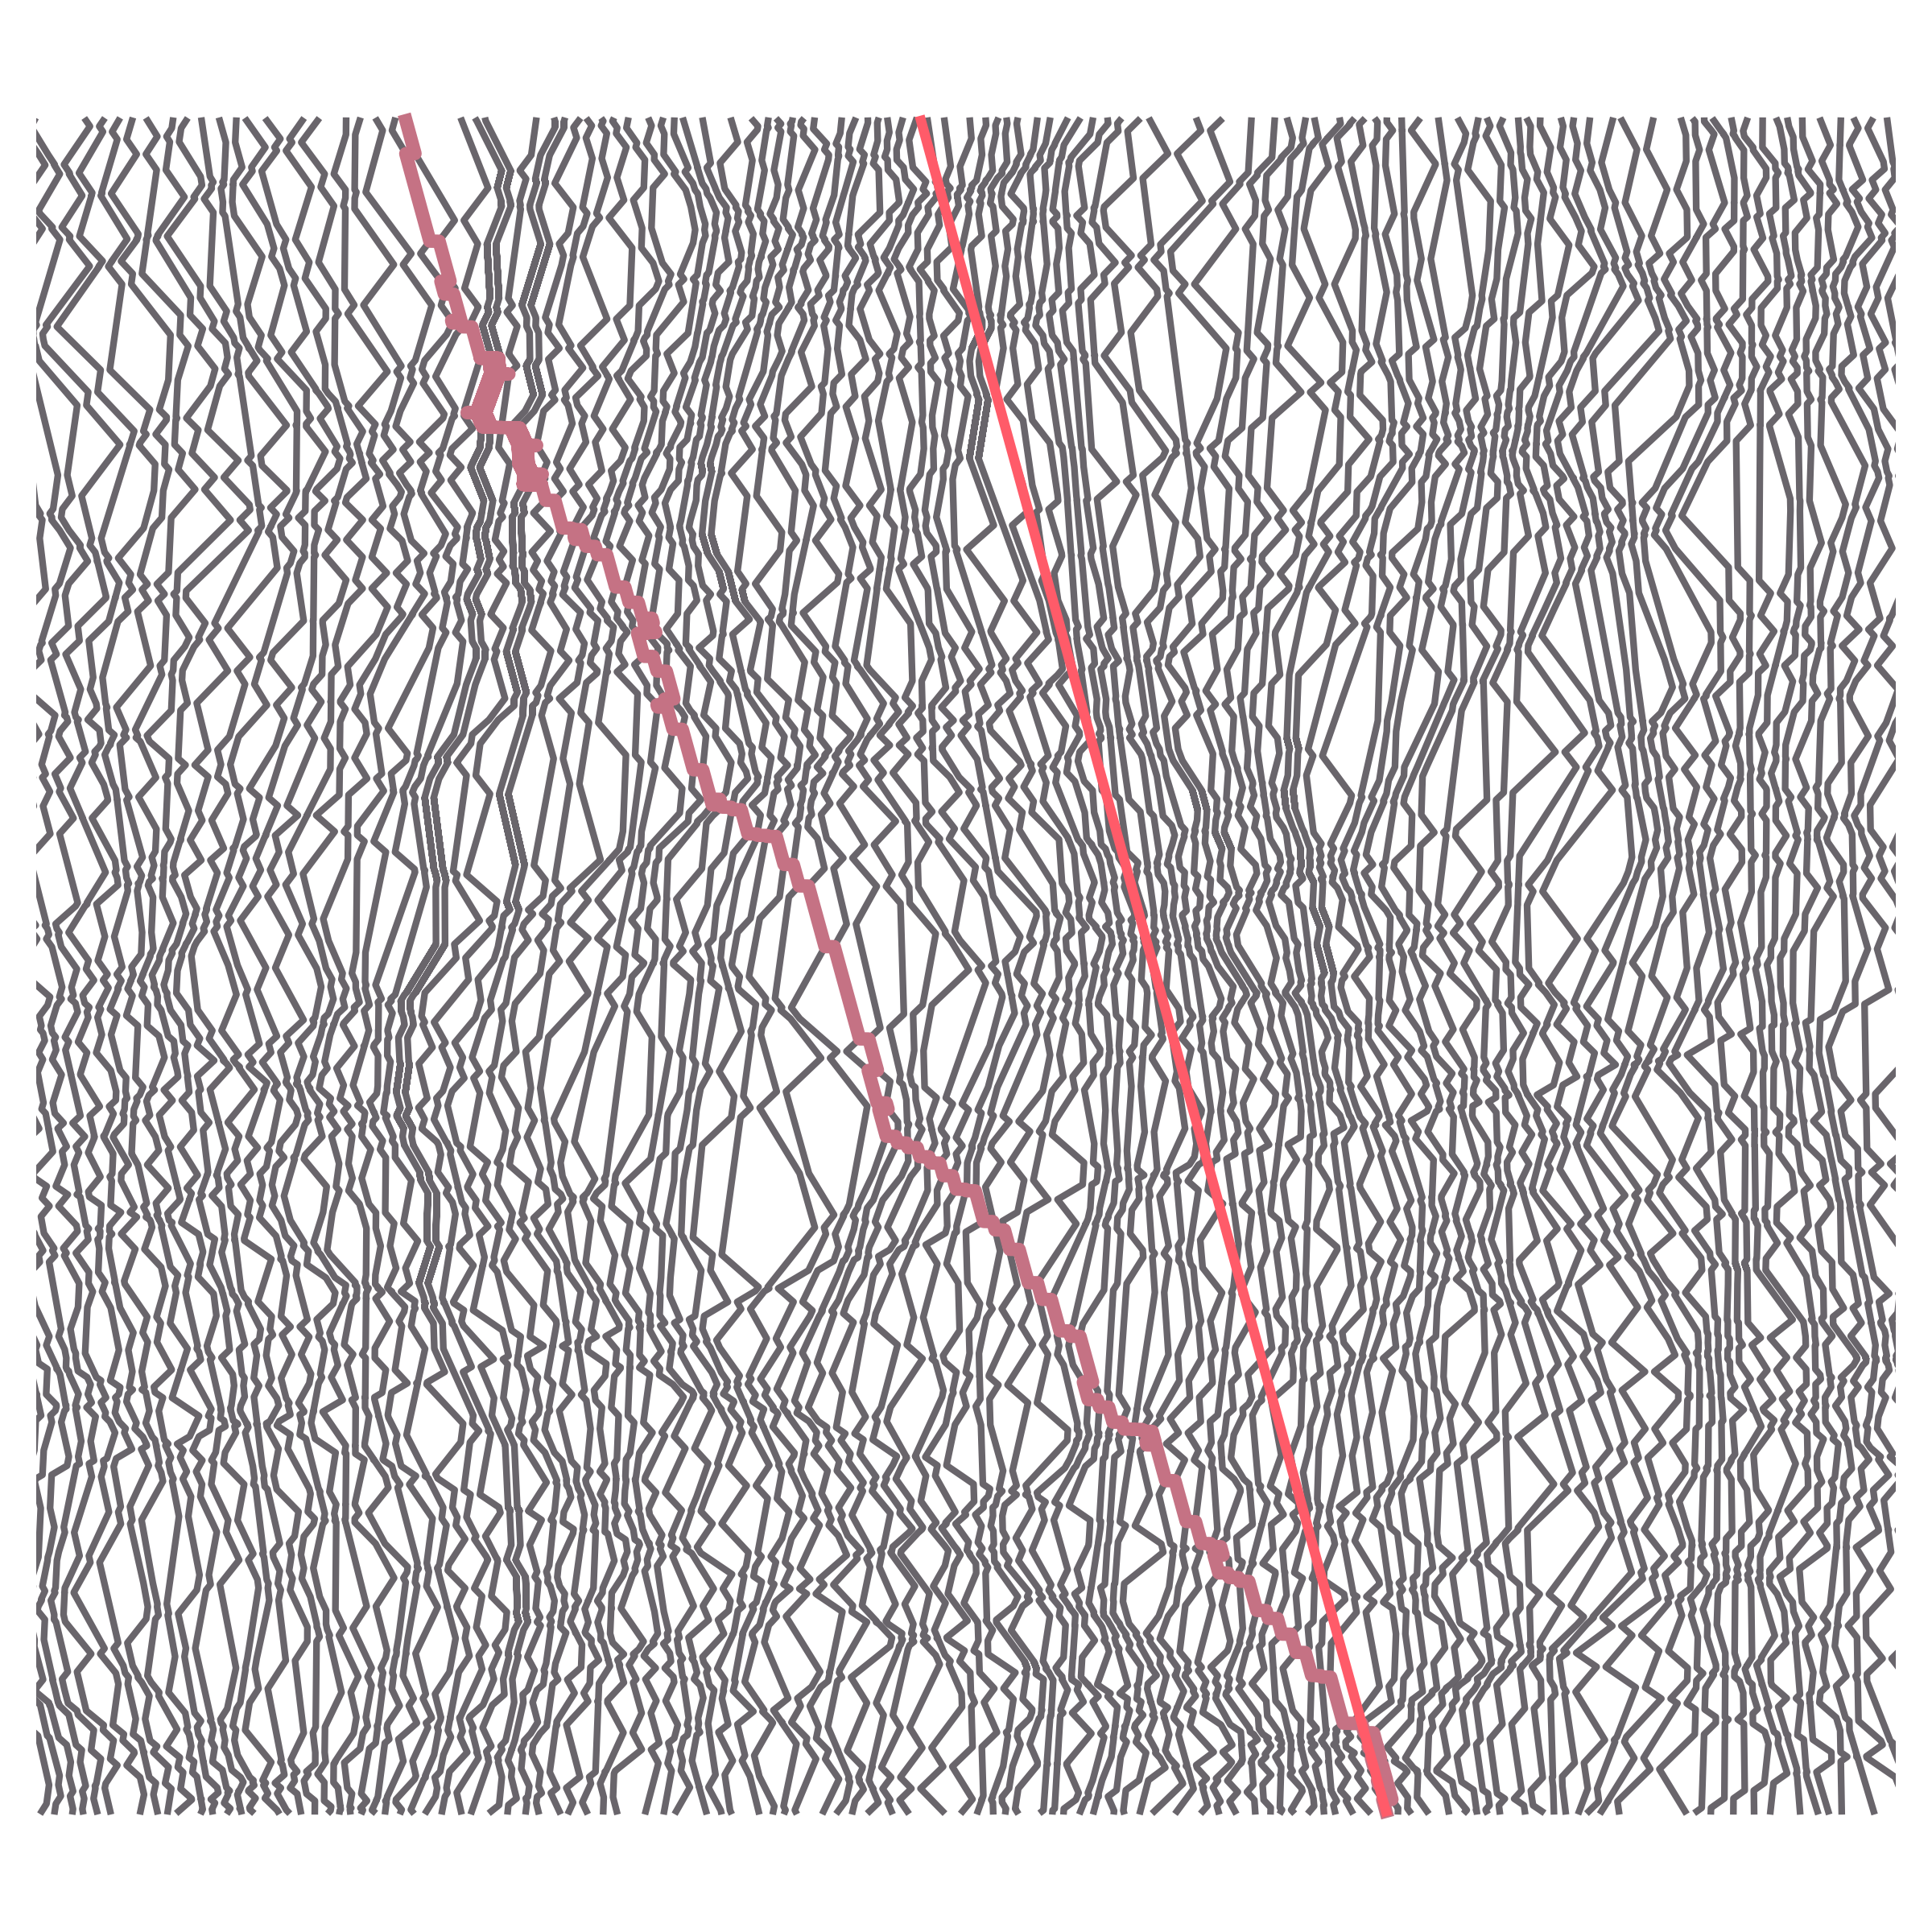
\includegraphics[width=0.8\textwidth]{figures/03_GHD/trajectoires_hard_rods.png}
    \caption{%Trajectoires des particules d'un gaz de hard rods en 1D. Les lignes noires représentent les particules individuelles, la ligne rouge correspond à la trajectoire effective (vitesse GHD) de la particule suivie, et la ligne orange indique la trajectoire de la particule si elle conservait sa vitesse initiale (bare velocity).
    Trajectoires des particules d'un gaz de barres dures en 1D. Les lignes noires représentent les particules individuelles, la ligne rouge la trajectoire effective (vitesse \gls{GHD}) de la particule suivie, et la ligne orange la trajectoire si la particule conservait sa vitesse initiale (bare velocity). Le graphique a été généré en Python.
    }
    \label{fig:trajectoires_hard_rods}
\end{figure}

\subsection{Diagonalisation et invariants de Riemann dans la GHD spatiale étendue}

%Nous nous restreignons au modèle de \gls{LL}.

%\medskip

En dérivant la définition de l'opération d’\emph{habillage} \eqref{eq:dressing}, on obtient la relation suivante :
\begin{equation}\label{chap:GHD:d.dressing.0}
	\partial_X \big( f^{\mathrm{dr}}_{[\nu]} \big) 
	= \partial_X f  +  \frac{\Delta}{2\pi} \star \big( \nu \, \partial_X f^{\mathrm{dr}}_{[\nu]} \big)  
	+ \frac{\Delta}{2\pi} \star \big( f^{\mathrm{dr}}_{[\nu]} \, \partial_X \nu \big), 	
\end{equation}
où les variables \(X \in \{  t, x, \theta \} \).  Soit 
% \begin{equation}\label{chap:GHD:d.dressing.0.0}
% 	\left ( 1 - \frac{\Delta}{2\pi} \star  \, \left ( \nu \, \times	 \, \right )  \right )  \partial_X \big( f^{\mathrm{dr}}_{[\nu]} \big) 
% 	= \partial_X f    
% 	+ \frac{\Delta}{2\pi} \star \big( f^{\mathrm{dr}}_{[\nu]} \, \partial_X \nu \big), 	
% \end{equation}
\begin{equation}\label{chap:GHD:d.dressing.0.0}
	\left(\mathrm{Id}-\widehat{K}_{\nu}\right) \partial_X \big( f^{\mathrm{dr}}_{[\nu]} \big) 
	= \partial_X f    
	+ \frac{\Delta}{2\pi} \star \big( f^{\mathrm{dr}}_{[\nu]} \, \partial_X \nu \big), 	
\end{equation}
% \left(\mathbb{1}-\widehat{K}_{[\nu]}\right)\partial_X f^{\mathrm{dr}}_{[\nu]},
% \left ( 1 - \frac{\Delta}{2\pi} \star  \left ( \nu \, \cdot	 \right )  \right )
où nous avons introduit l’opérateur linéaire \(\widehat{K}_{\nu}\) construit à partir de \(\big(\mathrm{Id}-\tfrac{\Delta}{2\pi}\star \nu \times \big)\) et de convolutions par \(\tfrac{\Delta}{2\pi}\) \ie 
\begin{equation}
	(\widehat{K}_{\nu} \,  g)(\theta) = \int d\theta'\, K_{\nu}(\theta,\theta') g(\theta'),\qquad K_{\nu}(\theta,\theta')=\frac{\Delta(\theta-\theta')}{2\pi}\,\nu(\theta').
\end{equation}



En utilisant la définition \eqref{eq:dressing}, on obtient également que 
\begin{equation}
	\big( \partial_X f \big)^{\mathrm{dr}}_{[\nu]} 
	= \left(\mathrm{Id}-\widehat{K}_{\nu}\right)^{-1} \partial_X f ,
\end{equation}
donc en injectant dans \eqref{chap:GHD:d.dressing.0.0} il vient que 
%\begin{equation}\label{chap:GHD:d.dressing.1}
%	\partial_X(f^{\mathrm{dr}}_{[\nu]}) = \left (\partial_X f \right )^{\mathrm{dr}}_{[\nu]} + \frac{\Delta}{2\pi} \star ( \nu (\partial_X f^{\mathrm{dr}}_{[\nu]}-\partial_X(f^{\mathrm{dr}}_{[\nu]})) )  +\frac{\Delta}{2\pi} \star ( f^{\mathrm{dr}}_{[\nu]} \partial_X \nu  ), 	
%\end{equation}
%
%comment ????
\begin{equation}\label{chap:GHD:d.dressing}
	\partial_X\!\left(f^{\mathrm{dr}}_{[\nu]}\right) 
	= \left(\partial_X f \right)^{\mathrm{dr}}_{[\nu]} 
	+ \widehat{\Theta} \!\left( f^{\mathrm{dr}}_{[\nu]} \,\partial_X \nu \right), 	
\end{equation}
% où \(X \in \{t, x, \theta\}\) et où nous avons introduit l’opérateur \(\Theta\) linéaire construit à partir de \(\left(\mathrm{Id}-\widehat{K}_{\nu}\right)^{-1}\) et de convolutions par \(\tfrac{\Delta}{2\pi}\) \ie
% \begin{equation}
% 	\Theta \equiv \left(Id-\widehat{K}_{\nu}\right)^{-1} 
% 	\, \frac{\Delta}{2\pi}\star
% \end{equation}

où \( X \in \{t, x, \theta\} \), et où nous avons introduit l’opérateur linéaire
\(\widehat{\Theta}\), défini comme la composition de l’inverse de l’opérateur
\(\mathrm{Id} - \widehat{K}_{\nu}\) avec la convolution par \(\tfrac{\Delta}{2\pi}\), \emph{i.e.}
\begin{equation}\label{eq:def_Theta}
    \widehat{\Theta}
    \;\doteq\;
    \left(\mathrm{Id} - \widehat{K}_{\nu}\right)^{-1}
    \circ
    \widehat{K}_{\mathrm{Id}},
\end{equation}
avec
\begin{equation}
	(\widehat{K}_{\mathrm{Id}} \,  g)(\theta) = \int d\theta'\, K_{\mathrm{Id}}(\theta,\theta') g(\theta'),\qquad K_{\mathrm{Id}}(\theta,\theta')=\frac{\Delta(\theta-\theta')}{2\pi}.
\end{equation}



\medskip
Les dérivations des équations \eqref{chap:GHD:eq.nu.v.a.1} donnent :
\begin{eqnarray}
	2\pi \partial_t \rho & = & 1^{\mathrm{dr}}_{[\nu]} \partial_t \nu + \nu \, \left (  ( \partial_t 1 )^{\mathrm{dr}}_{[\nu]}  + \widehat{\Theta} \left ( 1^{\mathrm{dr}}_{[\nu]} \partial_t \nu   \right ) \right )  \\
	2\pi \partial_x ( v^{\mathrm{eff}} \rho ) & = & (\partial_\theta h )^{\mathrm{dr}}_{[\nu]} \partial_x \nu + \nu \, \left (  ( \partial_x \partial_\theta h )^{\mathrm{dr}}_{[\nu]}  +  \widehat{\Theta} \left ( (\partial_\theta h)^{\mathrm{dr}}_{[\nu]} \partial_x \nu   \right ) \right )\\
	2\pi \partial_\theta ( a^{\mathrm{eff}} \rho ) & = & -(\partial_x h )^{\mathrm{dr}}_{[\nu]} \partial_\theta \nu - \nu \, \left (  ( \partial_\theta \partial_x h )^{\mathrm{dr}}_{[\nu]}  +  \widehat{\Theta} \left ( (\partial_x h)^{\mathrm{dr}}_{[\nu]} \partial_\theta \nu   \right ) \right )
\end{eqnarray}
%où \(\Theta\) est l'opérateur linéaire construit à partir de \(\big(1-\tfrac{\Delta}{2\pi}\star\nu\cdot\big)^{-1}\) et de convolutions par \(\tfrac{\Delta}{2\pi}\) (\ie $\(\Theta\) = \left ( 1 - \frac{\Delta}{2\pi} \star \nu \, \cdot	 \right )^{-1} \frac{\Delta}{2\pi} \star $ ) . 
En injectant  dans l'équation \gls{GHD} \eqref{chap:GHD:eq.GHD.1} on obtient après calculs (regroupement des termes et mise en facteur)  
%\begin{eqnarray}
%	\begin{array}{c}\left ( \left(\partial_t 1 \right)^{\mathrm{dr}} +  \left ( 1 + \left(\partial_x  \partial_\theta h  \right)^{\mathrm{dr}} - \left(\partial_\theta  \partial_x h  \right)^{\mathrm{dr}} \right ) \nu \, + \\ \left ( 1 + \left ( 1 -   \frac{\Delta}{2 \pi } \star \nu \cdot \right )^{-1} \frac{\Delta}{2 \pi } \star \right )   \left ( 1^{\mathrm{dr}} \partial_t v +  \left ( \partial_\theta h \right )^{\mathrm{dr}} \partial_x \nu -  \left ( \partial_x h \right )^{\mathrm{dr}} \partial_\theta \nu\right ) = 0  \end{array}. 
%\end{eqnarray}
\begin{eqnarray}
	\left ( \left(\partial_t 1 \right)^{\mathrm{dr}}  + \left(\partial_x  \partial_\theta h  \right)^{\mathrm{dr}} - \left(\partial_\theta  \partial_x h  \right)^{\mathrm{dr}} \right ) \nu \, + ( \mathrm{Id} + \widehat{\Theta} )    \left ( 1^{\mathrm{dr}} \partial_t v +  \left ( \partial_\theta h \right )^{\mathrm{dr}} \partial_x \nu -  \left ( \partial_x h \right )^{\mathrm{dr}} \partial_\theta \nu\right ) = 0  . 
\end{eqnarray}
Puisque \(\partial_t1=0\) et \(\partial_x\partial_\theta h=\partial_\theta\partial_x h\), le premier crochet s'annule. Il reste donc
\[
\Big(\mathrm{Id} + \widehat{\Theta} \Big)\Big( 1^{\mathrm{dr}}_{[\nu]}\,\partial_t\nu
+ (\partial_\theta h)^{\mathrm{dr}}_{[\nu]}\,\partial_x\nu
- (\partial_x h)^{\mathrm{dr}}_{[\nu]}\,\partial_\theta\nu \Big) = 0.
\]

Sous l'hypothèse standard d'inversibilité des opérateurs d'\emph{habillage} \Big (\ie\ \(\left(\mathrm{Id} - \widehat{K}_{\nu}\right)\)~ est inversible et \(\widehat{\Theta}\) n'a pas de noyau pathologique 
\footnote{
L'inversibilité de l'opérateur \(\left(\mathrm{Id} - \widehat{K}_{\nu}\right)\) est une condition technique garantissant que le système d'équations intégrales définissant l'opération de dressing possède une solution unique. En pratique, cela signifie que le noyau de convolution \(\tfrac{\Delta}{2\pi}\star\nu\) n'a pas de valeur propre égale à 1, ce qui assurerait une accumulation d'effets d'interaction menant à une singularité. Cette condition est généralement satisfaite pour les systèmes intégrables physiques dans les régimes d'intérêt (faibles densités, ou régimes thermodynamiquement stables). L'absence de noyau pathologique pour \(\widehat{\Theta}\) signifie quant à elle que cet opérateur ne possède pas de zéro du déterminant de Fredholm, assurant son caractère bien défini et injectif. Ces hypothèses standard permettent d'annuler le terme entre crochets dans l'équation précédente, conduisant ainsi à l'équation de transport \eqref{chap:GHD:eq.nu.1}.
} 
\Big ), on en déduit l'annulation du membre intérieur. En divisant par \(1^{\mathrm{dr}}_{[\nu]}\) on obtient l'équation de transport locale :
\begin{equation}\label{chap:GHD:eq.nu.1}
	\partial_t\nu + v^{\mathrm{eff}}\partial_x\nu + a^{\mathrm{eff}}\partial_\theta\nu = 0,
\end{equation}
(avec \(v^{\mathrm{eff}}=(\partial_\theta h)^{\mathrm{dr}}_{[\nu]}/1^{\mathrm{dr}}_{[\nu]}\) et \(a^{\mathrm{eff}}=-(\partial_x h)^{\mathrm{dr}}_{[\nu]}/1^{\mathrm{dr}}_{[\nu]}\)).  
  

\medskip

Dans les systèmes hyperboliques\footnote{
Un \emph{système hyperbolique} est un système d'équations aux dérivées partielles de la forme
\[
\partial_t \mathbf{u} + \mathbf{A}(x,t,\mathbf{u}) \cdot \partial_x \mathbf{u} = \mathbf{S}(x,t,\mathbf{u}),
\]
où $\mathbf{u}$ est un vecteur d'inconnues (ici les densités conservées ou les variables spectrales), $\mathbf{A}$ est une matrice (appelée matrice de flux ou jacobienne), et $\mathbf{S}$ représente les termes sources éventuels. Le système est dit \emph{hyperbolique} si la matrice $\mathbf{A}$ possède $N$ valeurs propres réelles distinctes (ou, plus généralement, réelles) et $N$ vecteurs propres linéairement indépendants. Cette structure assure que les perturbations se propagent à des vitesses finies et bien définies (les vitesses caractéristiques), ce qui permet une description dynamique stable et l'existence de solutions de type ondes. L'équation \gls{GHD}, avec ses vitesses effectives $v^{\mathrm{eff}}$ et $a^{\mathrm{eff}}$, possède cette structure hyperbolique, permettant ainsi une diagonalisation et l'identification des invariants de Riemann.
}, la \emph{diagonalisation} d'une équation consiste à trouver une transformation des variables qui permet de décomposer le système couplé en un ensemble de modes indépendants, appelés \emph{invariants de Riemann} ou \emph{modes normaux}. 


\medskip

Dans le cadre de la théorie \gls{GHD} spatiale étendue, l'équation d'évolution de la densité \(\rho(x,\theta,t)\) est couplée de manière non triviale en \((x,\theta)\) par la vitesse effective \(v^{\mathrm{eff}}\) et l'accélération effective \(a^{\mathrm{eff}}\). \footnote{Par « couplée de manière non triviale en $(x,\theta)$ » on entend que $\rho(x,\theta,t)$ ne se factorise pas en une dépendance séparée en $x$ et en $\theta$ : la valeur pour une rapidité donnée $\theta$ dépend des valeurs pour d'autres rapidités $\theta'$ (et parfois d'autres positions $x'$) via des opérateurs non locaux. Concrètement, le \emph{dressing} est un opérateur intégral qui couple toutes les composantes en $\theta$, par exemple
$$f^{\mathrm{dr}}(\theta)=f(\theta)+\int d\alpha\,T(\theta,\alpha)\,\nu(\alpha)\,f^{\mathrm{dr}}(\alpha),$$
ce qui signifie que $v^{\mathrm{eff}}$ et $a^{\mathrm{eff}}$ (qui sont construits à partir de quantités « dressed ») rendent l'évolution en $x$ pour une $\theta$ donnée dépendante de la distribution sur toutes les $\theta'$. Un « couplage trivial » serait, en revanche, une dépendance séparable ou purement locale (p.ex. $g(x)h(\theta)$).} 
La fonction d'occupation \(\nu(x,\theta ; t)\) est définie par une transformation non locale dite \emph{dressing} qui incorpore les interactions du système.




\medskip

Grâce à cela, on peut affirmer que la fonction $\nu (x , \theta)$  s’interprète comme un continuum d’{\bf invariants de Riemann}, c’est-à-dire des variables normales qui restent constantes le long des caractéristiques du système.\footnote{Par « restent constantes le long des caractéristiques du système », on entend que la valeur de $\nu(x,\theta;t)$ demeure inchangée lorsqu'on suit une particule (ou plus précisément une quasi-particule) le long de sa trajectoire dans l'espace $(x,\theta)$. Mathématiquement, cela s'exprime par $\frac{d\nu}{dt}\big|_{\text{caractéristique}} = 0$, où la dérivée est prise en suivant le mouvement selon les équations de transport \eqref{chap:GHD:eq.nu.1}. Autrement dit, même si $\nu(x,\theta;t)$ varie en fonction du temps et de la position lorsqu'on les observe en points fixes, elle reste constante le long des courbes caractéristiques définies par $\dot{x} = v^{\mathrm{eff}}(\theta)$ et $\dot{\theta} = a^{\mathrm{eff}}(x)$. C'est cette propriété qui fait de $\nu$ un véritable invariant de Riemann : chaque niveau de $\nu$ se propage selon ses propres caractéristiques sans se mélanger avec les autres niveaux, ce qui permet de diagonaliser entièrement la dynamique du système.}
En effet, l'équation de transport locale \eqref{chap:GHD:eq.nu.1} montre que \(\nu\) est conservée le long des trajectoires définies par les vitesses effectives \(v^{\mathrm{eff}}\) et les accélérations effectives \(a^{\mathrm{eff}}\). Autrement dit, chaque valeur de \(\nu\) pour une rapidité donnée \(\theta\) évolue indépendamment des autres, ce qui permet de diagonaliser le système d'équations couplées en un ensemble de modes indépendants.


\medskip

Cette diagonalisation \eqref{chap:GHD:eq.nu.1} est essentielle pour comprendre la structure hamiltonienne du système et simplifier l'analyse de sa dynamique, notamment dans le cadre spatialement étendu avec un dressing dépendant de la position. 
\footnote{
Par « diagonalisation », on entend le processus de transformation du système d'équations couplées \eqref{chap:GHD:eq.GHD.1} en un ensemble de modes découplés et indépendants. Dans le formalisme de la GHD, cela correspond à l'identification de la fonction d'occupation $\nu(x,\theta;t)$ comme un continuum d'invariants de Riemann. 

Mathématiquement, la diagonalisation s'exprime par le fait que l'équation de transport \eqref{chap:GHD:eq.nu.1}
\[
\partial_t\nu + v^{\mathrm{eff}}\partial_x\nu + a^{\mathrm{eff}}\partial_\theta\nu = 0
\]
peut être écrite sous la forme
\[
\frac{d\nu}{dt}\bigg|_{\text{car}} = 0,
\]
où la dérivée est prise le long des caractéristiques définies par $\dot{x} = v^{\mathrm{eff}}(\theta)$ et $\dot{\theta} = a^{\mathrm{eff}}(x)$. Cela signifie que chaque « niveau » de $\nu$ (chaque valeur de la fonction d'occupation pour une rapidité donnée) reste constant le long de sa trajectoire caractéristique dans l'espace $(x,\theta)$, sans se mélanger avec les autres niveaux. 

Cette propriété permet de résoudre le système complet non pas en tant que système couplé global, mais plutôt en suivant indépendamment l'évolution de chaque mode, ce qui simplifie drastiquement l'analyse dynamique même lorsque le dressing dépend explicitement de la position.
}

\section{Formulation hamiltonienne de la théorie Hydrodynamique Généralisée}

Dans  \cite{bonnemain2024hamiltonian}, il est montré que les équations \gls{GHD} peuvent
avoir une formulation Hamiltonienne dans le cadre d'une théorie de champ classique,
moyennant une redéfinition du crochet de Poisson. J'ai trouvé cette approche intéressante
et je présente ici ce résultat. En aucun cas les calculs ci-dessous ne sont une dérivation de \gls{GHD}.


\subsection{Crochet de Poisson fonctionnel}

% \paragraph{Interprétation et limite non-interactive}  
% À ce niveau de généralité, l'équation \gls{GHD} \eqref{chap:GHD:eq.GHD.1} peut être interprétée comme la dynamique hydrodynamique d’un fluide bidimensionnel dont la densité est conservée dans l’espace des phases spectral.  
% Les effets d’interaction se traduisent par un couplage non local dans la direction des rapidités $\theta$, reflétant les processus d'interactions entre quasi-particules possédant des paramètres spectraux distincts.

\paragraph{Interprétation et limite non-interactive}  
À ce niveau de généralité, l'équation \gls{GHD} \eqref{chap:GHD:eq.GHD.1} peut être interprétée comme la dynamique hydrodynamique d'un fluide bidimensionnel\footnote{Le terme « bidimensionnel » désigne ici l'espace des phases spectral $(x,\theta)$, et non l'espace physique. Les deux dimensions correspondent à : (i) la variable spatiale $x$ décrivant l'inhomogénéité du système dans l'espace physique réel, et (ii) la variable spectrale $\theta$ (la rapidité) caractérisant l'état asymptotique de chaque quasi-particule. La « densité » dans cet espace $(x,\theta)$ est précisément $\rho(x,\theta,t)$, la distribution locale de rapidité.} dont la densité est conservée dans l'espace des phases spectral.  
Les effets d'interaction se traduisent par un couplage non local dans la direction des rapidités $\theta$\footnote{Le « couplage non local en $\theta$ » signifie que l'évolution de $\rho(x,\theta,t)$ pour une rapidité donnée $\theta$ dépend non seulement de la distribution aux points voisins en $\theta$, mais aussi de la distribution sur l'ensemble du spectre de rapidités. Mathématiquement, cela se manifeste par des opérateurs intégraux, notamment le dressing $(\cdot)^{\mathrm{dr}}_{[\nu]}$ (équation \eqref{eq:dressing}), qui couple implicitement toutes les valeurs de $\theta'$ à travers des noyaux de convolution comme $\Delta(\theta-\theta')$ (voir équation \eqref{chap:GHD:veff.4}). Cette non-localité reflète le fait que, dans un système intégrable, les interactions à deux corps entre quasi-particules de rapidités différentes créent un couplage global : une quasi-particule à la rapidité $\theta$ « ressent » la présence de toutes les autres quasi-particules à d'autres rapidités $\theta'$, et sa dynamique en est affectée de façon non triviale.}, reflétant les processus d'interactions entre quasi-particules possédant des paramètres spectraux distincts\footnote{Par « paramètres spectraux distincts », on entend que deux quasi-particules ont des rapidités différentes, $\theta \neq \theta'$. Dans un système intégrable, les collisions binaires entre quasi-particules de rapidités différentes sont décrites par la matrice de diffusion (ou matrice $S$), caractérisée par la phase de diffusion $\varphi(\theta - \theta')$ ou le noyau de dressing $\Delta(\theta-\theta')$. Ces grandeurs dépendent de la différence relative des rapidités et encodent comment la présence d'une quasi-particule à rapidité $\theta'$ modifie le comportement effectif d'une quasi-particule à rapidité $\theta$. C'est précisément cette interaction sélective entre différents « modes » spectraux qui crée le couplage non local observable dans l'équation \gls{GHD}.}.

\medskip

Dans le cas limite d’un système \emph{sans interactions}, l’espace spectral coïncide avec l’espace des phases classiques, et l’équation \gls{GHD} se réduit alors à l’équation de Liouville (ou, de façon équivalente, à l’équation de Boltzmann sans terme de collisions) issue de la théorie cinétique élémentaire.

\medskip

En l’absence de phénomènes dissipatives, la densité de distribution $\rho$ est conservée le long du flot hamiltonien associé à l’énergie $H$, ce qui s’exprime par
\footnote{
	\textbf{Convention de signe pour l'équation de Liouville et le crochet de Poisson~:}
	Il existe deux conventions couramment utilisées dans la littérature. 
	La convention de \textbf{Dirac} (adoptée dans ce chapitre) définit l'équation de Liouville comme
	\[
	\frac{d\rho}{dt} = \frac{\partial\rho}{\partial t} + \{\rho, H\} = 0,
	\]
	où le crochet de Poisson canonique est $\{A,B\} = \sum_i \left(\frac{\partial A}{\partial q_i}\frac{\partial B}{\partial p_i} - \frac{\partial A}{\partial p_i}\frac{\partial B}{\partial q_i}\right)$.
	La convention de \textbf{Landau et Lifschitz} utilise une définition opposée du crochet, conduisant à $\frac{d\rho}{dt} = \frac{\partial\rho}{\partial t} - \{\rho, H\} = 0$.
	Ces deux formulations sont équivalentes mathématiquement, mais diffèrent par le signe du crochet de Poisson. 
	Dans ce manuscrit, nous suivons la convention de \textbf{Dirac}.
}
\begin{equation}\label{chap:GHD:eq.Liouv.1}
	\frac{d \rho}{dt} 
	= \frac{\partial \rho}{\partial t } + \{ \rho , H \} = 0,
\end{equation}
où $\{\bullet, \bullet\}$ désigne le crochet de Poisson canonique dans l’espace des phases.  
Dans cette perspective, la théorie \gls{GHD} apparaît comme une extension naturelle de l’équation de Liouville aux systèmes intégrables, incorporant les effets collectifs induits par les interactions tout en préservant une description exacte à grande échelle.\footnote{La théorie \gls{GHD} fournit, pour les modèles intégrables, une description rigoureuse de la dynamique à l'échelle d'Euler. Elle n'est pas une approximation de type champ moyen : elle résulte de la prise en compte explicite de l'infinité de lois de conservation caractéristiques de l'intégrabilité et, de ce fait, préserve la structure des corrélations et l'ensemble des charges conservées. Elle établit un lien cohérent entre la dynamique microscopique — l'évolution des quasi‑particules en variables spectrales \(\theta\) et spatiales \(x\) — et la dynamique macroscopique des densités résolues en rapidité, sans recours à des termes phénoménologiques intermédiaires. Enfin, dans la limite sans interactions l'espace spectral coïncide avec l'espace des phases classique et l'équation \gls{GHD} se réduit à l'équation de Liouville (équivalente à la formulation cinétique collisionless, p.ex. Vlasov/Boltzmann sans terme de collision).}


\paragraph{Structure hamiltonienne et crochet de Poisson fonctionnel}  
Bonnemain \emph{et al.} \cite{bonnemain2024hamiltonian} introduisent un crochet de Poisson fonctionnel agissant sur des fonctionnelles $F$ et $G$ de la distribution de rapidité $\rho(x,\theta)$ en présence d’interactions. Celui-ci s’écrit
\begin{equation}\label{chap:GHD:eq.chochet.bonnemain.1}
	\{F,G\}
	=\iint dx\,d\theta\;\frac{\nu}{2\pi}\,
	\left[
		\partial_x \left( \frac{\delta F}{\delta \rho(x,\theta)} \right)
		\left( \partial_\theta \left( \frac{\delta G}{\delta \rho(x,\theta)} \right) \right)^{\mathrm{dr}}_{[\nu]}
		-
		\partial_x \left( \frac{\delta G}{\delta \rho(x,\theta)} \right)
		\left( \partial_\theta \left( \frac{\delta F}{\delta \rho(x,\theta)} \right) \right)^{\mathrm{dr}}_{[\nu]}
	\right],
\end{equation}
où $\nu$ désigne la fonction d’occupation. Dans ce crochet l'application de l’opération d’\emph{habillage} $(\bullet)^{\mathrm{dr}}_{[\nu]}$ \eqref{eq:dressing}  traduit les interactions entre particules.

%L’opérateur de \emph{dressing} $(\cdot)^{\mathrm{dr}}_{[\nu]}$ agit ici sur les dérivées fonctionnelles dans la variable spectrale $\theta$ ; il encode les effets des interactions à longue portée dans l’espace des rapidités. Cette structure hamiltonienne permet de reformuler la GHD comme une équation de type Liouville sur l’espace fonctionnel des distributions $\rho$, mais avec un crochet de Poisson modifié par le \emph{dressing}, traduisant la nature intégrable et non-locale des interactions.

\medskip


Le crochet de Poisson (défini en~\eqref{chap:GHD:eq.chochet.bonnemain.1}) entre deux charges $\mathcal{Q}[f]$ et $\mathcal{Q}[g]$ prend la forme
\begin{equation}\label{chap:GHD:eq.chochet.bonnemain.2}
	\{\mathcal{Q}[f], \mathcal{Q}[g]\}
	= \int_{\mathbb{R}^2} dx\, d\theta\, \frac{\nu}{2\pi} 
	\left[ \partial_x f \, (\partial_\theta g)^{\mathrm{dr}}_{[\nu]} 
	     - \partial_x g \, (\partial_\theta f)^{\mathrm{dr}}_{[\nu]} \right].
\end{equation}
%où $\nu$ est la fonction d’occupation et $(\cdot)^{\mathrm{dr}}_{[\nu]}$ désigne l’application de \emph{dressing} associée à $\nu$.

\medskip

Cette application de \emph{dressing} satisfait la relation de symétrie~\cite{doyon2020lecture} :
\begin{equation}\label{chap:GHD:eq.sym.dr.1}
	\int_{\mathbb{R}^2} dx\, d\theta \; \nu \, f \, g^{\mathrm{dr}}_{[\nu]} 
	= \int_{\mathbb{R}^2} dx\, d\theta \; \nu \, f^{\mathrm{dr}}_{[\nu]} \, g.
\end{equation}

%Pour appliquer la relation de symétrie~\eqref{chap:GHD:eq.sym.dr.1} au crochet~\eqref{chap:GHD:eq.chochet.bonnemain.2}, il est nécessaire de vérifier que les fonctions impliquées satisfont les conditions requises sur leurs types tensoriels.
%\footnote{
%La relation de symétrie~\eqref{chap:GHD:eq.sym.dr.1} est valable lorsque la somme des types tensoriels de $f$ et $g$ est $(1,1)$ dans le sens de~\cite{doyon2020lecture}. Dans ce formalisme, le type $(a,b)$ caractérise la transformation d'un objet vis-à-vis de $x$ (première entrée) et de $\theta$ (seconde entrée). Si $f$ est de type $(p,q)$ et $g$ de type $(r,s)$, alors leur somme est $(p+r,q+s)$. La condition $(1,1)$ garantit que l'intégrande $\nu\, f\, g^{\mathrm{dr}}$ est un scalaire invariant, rendant l'intégrale bien définie. Dans~\eqref{chap:GHD:eq.chochet.bonnemain.2}, $\partial_x f$ est de type $(1,0)$ et $\partial_\theta g$ de type $(0,1)$, ce qui satisfait cette condition et permet l'utilisation de~\eqref{chap:GHD:eq.sym.dr.1}.
%}

Pour appliquer la relation de symétrie~\eqref{chap:GHD:eq.sym.dr.1} au crochet~\eqref{chap:GHD:eq.chochet.bonnemain.2}, il suffit de considérer que les fonctions impliquées $f$ et $g$ sont des fonctions scalaires régulières sur $(x,\theta)$. Dans ce cas, la relation de symétrie reste pleinement valide et l'intégrale est bien définie.

\footnote{La relation de symétrie~\eqref{chap:GHD:eq.sym.dr.1} stipule que 
\begin{equation*}
\int_{\mathbb{R}^2} dx\, d\theta \; \nu \, f \, g^{\mathrm{dr}}_{[\nu]} 
= \int_{\mathbb{R}^2} dx\, d\theta \; \nu \, f^{\mathrm{dr}}_{[\nu]} \, g,
\end{equation*}
ce qui signifie que l'intégrale double sur l'espace $(x,\theta)$ du membre de gauche égale celle du membre de droit. Cette symétrie de l'opérateur de dressing permet d'échanger l'action du dressing entre $g$ et $f$ à travers l'intégration, ce qui est crucial pour réduire le crochet~\eqref{chap:GHD:eq.chochet.bonnemain.2} à la forme compacte~\eqref{chap:GHD:eq.chochet.bonnemain.3}. Le formalisme des types tensoriels introduit dans~\cite{doyon2020lecture} sert à traiter des objets plus complexes (tenseurs dépendant de $x$ et $\theta$); pour des fonctions scalaires comme ici, aucune condition supplémentaire n'est nécessaire.}

En utilisant cette symétrie ainsi qu’une intégration par parties, le crochet~\eqref{chap:GHD:eq.chochet.bonnemain.2} se réécrit
\begin{equation}\label{chap:GHD:eq.chochet.bonnemain.3}
	\{\mathcal{Q}[f], \mathcal{Q}[g]\}
	= \int_{\mathbb{R}^2} dx\, d\theta \; f \,
	\left[
		\partial_\theta \left( \frac{\nu}{2\pi} \, (\partial_x g)^{\mathrm{dr}}_{[\nu]} \right)
		- \partial_x \left( \frac{\nu}{2\pi} \, (\partial_\theta g)^{\mathrm{dr}}_{[\nu]} \right)
	\right].
\end{equation}

\medskip

\subsection{Crochet avec l’Hamiltonien}

On reprend un Hamiltonien de la forme de \eqref{chap:GHD:eq.ham.1},  $H = \mathcal{Q}[h]$. 

\paragraph{Densité hamiltonienne et grandeurs effectives} 
%On note $h(x,\theta)$ la densité associée à la moyenne de l’Hamiltonien, telle que
%\begin{equation}\label{chap:GHD:eq.ham.1}
%	H = \mathcal{Q}[h].
%\end{equation}

%La fonction d’occupation $\nu$, la vitesse effective $v^{\mathrm{eff}}$ et l’accélération effective $a^{\mathrm{eff}}$ sont définies par
%\begin{equation}\label{chap:GHD:eq.nu.v.a.1}
%	\nu = 2\pi \frac{\rho}{1^{\mathrm{dr}}_{[\nu]}}, 
%	\quad v^{\mathrm{eff}} = \frac{(\partial_\theta h )^{\mathrm{dr}}_{[\nu]}}{1^{\mathrm{dr}}_{[\nu]}}, 
%	\quad a^{\mathrm{eff}} = -\frac{(\partial_x h )^{\mathrm{dr}}_{[\nu]}}{1^{\mathrm{dr}}_{[\nu]}},
%\end{equation}
%\begin{equation}\label{chap:GHD:eq.nu.v.a.1}
%	2 \pi \rho =  1^{\mathrm{dr}}_{[\nu]} \, \nu , 
%	\quad 2 \pi \, v^{\mathrm{eff}} \, \rho  =(\partial_\theta h )^{\mathrm{dr}}_{[\nu]} \, \nu , 
%	\quad 2 \pi \, a^{\mathrm{eff}} \, \rho  = -(\partial_x h )^{\mathrm{dr}}_{[\nu]}\, \nu ,
%\end{equation}
%toutes trois étant des fonctions de $\rho(\cdot,\cdot,t)$. 

% La vitesse effective et l'accélération effective données à l'équation \eqref{chap:GHD:eq.nu.v.a.1} interviennent dans les équations de mouvement
% \begin{equation}\label{chap:GHD:eq.nu.v.a.1.1}
% 	\dot{x} = v^{\mathrm{eff}}, \qquad \dot{\theta} = a^{\mathrm{eff}},
% \end{equation}
% montrant que les dérivées $\partial_x$ et $\partial_\theta$ présentes dans le crochet de Poisson correspondent respectivement à l'action de l'accélération effective sur $\theta$ et de la vitesse effective sur $x$.

\medskip

La vitesse effective et l'accélération effective données à l'équation \eqref{chap:GHD:eq.nu.v.a.1} interviennent dans les équations de mouvement\footnote{Ces équations de mouvement découlent de la structure hamiltonienne du système. Elles expriment que les variables conjuguées $x$ et $\theta$ évoluent selon les vitesses et accélérations effectives, qui encodent la dynamique complète du système dans le référentiel considéré.}
\begin{equation}\label{chap:GHD:eq.nu.v.a.1.1}
    \dot{x} = v^{\mathrm{eff}}, \qquad \dot{\theta} = a^{\mathrm{eff}},
\end{equation}
montrant que les dérivées $\partial_x$ et $\partial_\theta$ présentes dans le crochet de Poisson %$\{A, B\} = \partial_x A \partial_\theta B - \partial_\theta A \partial_x B$ 
correspondent respectivement aux générateurs infinitésimaux de l'évolution temporelle. Plus précisément :
\begin{itemize}[label = $\bullet$ ]
    \item $\partial_x$ agit comme le générateur des translations en $\theta$ via l'accélération effective $a^{\mathrm{eff}}$ ;
    \item $\partial_\theta$ agit comme le générateur des translations en $x$ via la vitesse effective $v^{\mathrm{eff}}$.
\end{itemize}
Ainsi, le crochet de Poisson encode le couplage entre ces deux degrés de liberté à travers les termes effectifs.

\medskip 

%Avec ces définitions, le crochet~\eqref{chap:GHD:eq.chochet.bonnemain.3} s’écrit
En utilisant la définition de $v^{\mathrm{eff}}$ et $a^{\mathrm{eff}}$ données à l'équation \eqref{chap:GHD:eq.nu.v.a.1}, on trouve que le crochet \eqref{chap:GHD:eq.chochet.bonnemain.3} appliqué à $(f,h)$ devient 
\begin{equation}\label{chap:GHD:eq.chochet.bonnemain.4}
	\{\mathcal{Q}[f], \mathcal{Q}[h]\} 
	= - \int_{\mathbb{R}^2} dx\, d\theta \; f \left[ \partial_x \big( \rho \, v^{\mathrm{eff}} \big) 
	+ \partial_\theta \big( \rho \, a^{\mathrm{eff}} \big) \right].
\end{equation}

\paragraph{Forme locale : densités conservées .} 
En choisissant $(x,\theta) \mapsto \delta(\cdot - x)f(\theta)$ dans \eqref{chap:GHD:eq.charge.global.1}, on obtient la moyenne de la densité conservée \ie
%On remarque que les moyennes des densités conservées $q_{[f]}(x)$ s’obtiennent en appliquant la prescription
%\[
%(x,\theta) \mapsto \delta(\cdot - x) \, f(\theta)
%\]
%dans~\eqref{chap:GHD:eq.charge.global.1}, \emph{i.e.}
\begin{equation}\label{chap:GHD:eq.chochet.bonnemain.4.11}
	q_{[f]}(x,t) = \mathcal{Q} \big[ (x,\theta) \mapsto \delta(\cdot - x) \, f(\theta) \big] =\int d\theta\, f(\theta)\,\rho(x,\theta,t).
\end{equation}

Appliqué à~\eqref{chap:GHD:eq.chochet.bonnemain.4}, on obtient
\begin{equation}\label{chap:GHD:eq.chochet.bonnemain.5}
	\{q_{[f]}(x), \mathcal{Q}[h]\} 
	= - \partial_x \left[ \int_{\mathbb{R}} d\theta \; f \, \rho \, v^{\mathrm{eff}} \right]
	+ \int_{\mathbb{R}} d\theta \; f' \, \rho \, a^{\mathrm{eff}}.
\end{equation}

En appliquant l’équation de Liouville~\eqref{chap:GHD:eq.Liouv.1} , on retrouve la forme de convection~\eqref{chap:GHD:eq.conserv.1} :
\begin{equation}\label{chap:GHD:eq.conserv.2}
	\partial_t q_{[f]} + \partial_x j_{[f]} = F_{[f]},
\end{equation}
où le flux $j_{[f]}$ et le terme de force $F_{[f]}$ sont donnés par
\begin{equation}\label{chap:GHD:eq.conserv.2.1}
	j_{[f]} = \int_{\mathbb{R}} d\theta \; v^{\mathrm{eff}} \, f \, \rho,
	\quad F_{[f]} = \int_{\mathbb{R}} d\theta \; a^{\mathrm{eff}} \, f' \, \rho.
\end{equation}

\paragraph{Forme locale : équation sur \texorpdfstring{$\rho$}{rho}} 
De manière analogue, pour la distribution de rapidité à l’équilibre thermodynamique, on note
\begin{equation}
	\rho(x,\theta) = \mathcal{Q}\big[ \delta(\cdot - x) \, \delta(\cdot - \theta) \big].
\end{equation}
Appliqué à~\eqref{chap:GHD:eq.chochet.bonnemain.4}, on obtient
\begin{equation}\label{chap:GHD:eq.chochet.bonnemain.6}
	\{\rho(x,\theta), \mathcal{Q}[h]\} 
	= - \partial_x \big( v^{\mathrm{eff}} \, \rho \big)
	  - \partial_\theta \big( a^{\mathrm{eff}} \, \rho \big).
\end{equation}

% En appliquant l’équation de Liouville~\eqref{chap:GHD:eq.Liouv.1}, on retrouve l’équation \gls{GHD}~\eqref{chap:GHD:eq.GHD.1} :
% \begin{equation*}\label{chap:GHD:eq.conserv.3}
% 	\partial_t \rho + \partial_x \big( v^{\mathrm{eff}} \rho \big)
% 	+ \partial_\theta \big( a^{\mathrm{eff}} \rho \big) = 0.
% \end{equation*}

{\color{blue}
En appliquant l’équation de Liouville~\eqref{chap:GHD:eq.Liouv.1} ($\partial_t \rho(x,\theta,t) = \{\rho(x,\theta,t), H\}$), on retrouve l’équation \gls{GHD}~\eqref{chap:GHD:eq.GHD.1}%\footnote{Remarque sur la convention de signe~: nous utilisons ici la convention \(\dfrac{d\rho}{dt}=\partial_t\rho+\{\rho,H\}=0\) (voir \eqref{chap:GHD:eq.Liouv.1}); avec le crochet de Poisson défini en \eqref{chap:GHD:eq.chochet.bonnemain.1} cela conduit précisément au signe présent dans \eqref{chap:GHD:eq.chochet.bonnemain.6}, il n'y a donc pas d'erreur de signe.} 
:
\begin{equation*}\label{chap:GHD:eq.conserv.3}
	\partial_t \rho + \partial_x \big( v^{\mathrm{eff}} \rho \big)
	+ \partial_\theta \big( a^{\mathrm{eff}} \rho \big) = 0.
\end{equation*}

}




%\section{Cas particuliers et interpretations}
\subsection{Modèle de Lieb–Liniger}

%Les informations relatives aux interactions entre particules sont contenues dans la définition du crochet de Poisson \eqref{chap:GHD:eq.chochet.bonnemain.1}, associée à l’opérateur de \emph{dressing} spécifique au modèle de Lieb–Liniger, défini en \eqref{eq:dessing}.  
Dans le modèle de \gls{LL}, l’Hamiltonien $H = \mathcal{Q}[h]$ \eqref{chap:GHD:eq.ham.1} s’écrit ici avec :
\begin{equation}\label{chap:GHD:eq.ham.2}
	h(x , \theta ) = \varepsilon(\theta) + V(x),
\end{equation}
où l’énergie cinétique est $\varepsilon(\theta) = \theta^2 / 2$ et $V(x)$ représente le potentiel extérieur.

\medskip

Dans ce modèle, la vitesse effective et l’accélération effective de \eqref{chap:GHD:eq.nu.v.a.1} se réécrivent :
\begin{equation}\label{chap:GHD:eq.nu.v.a.1.1111}
	v^{\mathrm{eff}} = \frac{(\mathrm{Id})^{\mathrm{dr}}_{[\nu]}}{1^{\mathrm{dr}}_{[\nu]}}, 
	\quad a^{\mathrm{eff}} = - V'(x).
\end{equation}

Avec l'equation \eqref{chap:GHD:veff.4} la vitesse effectif dans le modèle de \gls{LL} vérifie : 
\begin{equation}
	v^{\mathrm{eff}} = \theta +	\int d \theta' \, \Delta(\theta - \theta') \rho ( \theta') ( v^{\mathrm{eff}} ( \theta' ) - v^{\mathrm{eff}} ( \theta )  ) 
\end{equation}


Ainsi, les termes de force dans \eqref{chap:GHD:eq.conserv.2} et \eqref{chap:GHD:eq.conserv.2.1} prennent la forme :
\begin{equation}
	F_{[f]} = -V'(x) \int_{\mathbb{R}} d\theta \, f'(\theta) \, \rho(x, \theta).
\end{equation}

L’équation GHD \eqref{chap:GHD:eq.GHD.1} devient alors :
\begin{equation}\label{chap:GHD:eq.conserv.3.1}
	\partial_t \rho + \partial_x\!\left(v^{\mathrm{eff}} \rho\right) - V'(x) \, \partial_\theta \rho = 0,
\end{equation}
et \eqref{chap:GHD:eq.nu.1} devient :
\begin{equation}\label{chap:GHD:eq.nu.1.1}
	\partial_t \nu + v^{\mathrm{eff}}\partial_x \nu - V'(x) \, \partial_\theta \rho = 0,
\end{equation}



%\subsection{Cas sans interaction}
%
%\paragraph{Hypothèse ``sans interactions'' : $^{\rm dr}=\mathrm{Id}$.}
%Si l’opérateur d’habillage est l’identité (\emph{no dressing}), les crochet \eqref{chap:GHD:eq.chochet.bonnemain.1} et \eqref{chap:GHD:eq.chochet.bonnemain.4} se simplifient en :

\subsection{Cas ``no dressing''}

\paragraph{Hypothèse ``opérateur d’habillage identité'' : $^{\rm dr}=\mathrm{Id}$.}  
Si l’opérateur d’habillage correspond à l’identité (\emph{no dressing}), les crochets \eqref{chap:GHD:eq.chochet.bonnemain.1} et \eqref{chap:GHD:eq.chochet.bonnemain.4} se simplifient en :
\begin{eqnarray}
	\{F,G\} & = &  \iint dx\,d\theta\;\rho \,\left[\partial_x \!\left( \frac{\delta F}{\delta \rho (x , \theta)} \right)\, \partial_\theta \!\left( \frac{\delta G}{\delta \rho (x , \theta)} \right) - \partial_x \!\left( \frac{\delta G}{\delta \rho (x , \theta)} \right) \, \partial_\theta \!\left( \frac{\delta F}{\delta \rho(x , \theta) } \right) \right],\\
	\{\mathcal{Q}[f], \mathcal{Q}[h]\} &=& - \int_{\mathbb{R}^2} dx\, d\theta \; f \left[ \partial_x \big( \rho \, v^{\mathrm{eff}} \big) 
	+ \partial_\theta \big( \rho \, a^{\mathrm{eff}} \big) \right].
\end{eqnarray}
Les flux et termes de force \eqref{chap:GHD:eq.conserv.2.1} s’expriment alors en remplaçant la vitesse effective $v^{\mathrm{eff}}$ et l’accélération effective $a^{\mathrm{eff}}$ (de \eqref{chap:GHD:eq.nu.v.a.1}) par leurs expressions issues de la dynamique hamiltonienne \emph{nue} :
\begin{equation}
	\nu = 2\pi \rho, \qquad v^{\rm eff}(\theta)\ \to\ \partial_\theta h(x,\theta), \qquad a^{\rm eff}(\theta)\ \to\ -\partial_x h(x,\theta),
\end{equation}
où $h(x,\theta)$ est l’hamiltonien \emph{nu} (par exemple $h=\varepsilon(\theta)+V(x)$). 
Dans la limite sans interactions, l’équation \eqref{chap:GHD:eq.GHD.1} se réduit à une équation de transport sans collisions (de type Vlasov) :
\footnote{L'équation de Vlasov décrit l'évolution d'une distribution de particules dans l'espace des phases, en tenant compte des interactions entre particules. Elle est souvent utilisée pour modéliser des systèmes de particules dans des contextes où les effets de collision peuvent être négligés, permettant ainsi d'étudier la dynamique des systèmes en équilibre ou quasi-équilibre.}
\begin{equation}\label{eq:transport-libre}
  \partial_t \rho + \partial_x\!\big( \partial_\theta h\ \rho \big)
  - \partial_\theta\!\big( \partial_x h\ \rho \big) = 0.
\end{equation}

\paragraph{Hiérarchie des moments (charges nues).}
Pour toute fonction test $f(\theta)$, l'équation \eqref{chap:GHD:eq.chochet.bonnemain.5} devient
\begin{eqnarray}\label{chap:GHD:eq.flux.1}
j_{[f]}(x,t)=\int d\theta\, f(\theta)\,\partial_\theta h\,\rho(x,\theta,t), \qquad F_{[f]}(x,t) = -\int_{\mathbb{R}} d\theta \; \partial_x h \, f'(\theta)  \, \rho(x,\theta,t).
\end{eqnarray}

Pour $f(\theta) = 1$, $\theta$ et $\theta^2/2$ et $h(\theta,x)=\varepsilon(\theta)+V(x)$, l'équation \eqref{chap:GHD:eq.conserv.2} avec la charge locale \eqref{chap:GHD:eq.chochet.bonnemain.4.11} et les flux et forces \eqref{chap:GHD:eq.flux.1}, déviennent les équations d’Euler classiques (Annexe \ref{annex:Euler}) :
\begin{eqnarray}\label{chap:3:eq:hydro.1}
	\left\{
	\begin{array}{rcl}
	\partial_t n + \partial_x (n u) &=& 0, \\
	\partial_t (n u) + \partial_x (nu^2 + \mathcal{P}) &=& -\, n\partial_x V(x), \\
	\partial_t E + \partial_x (u\,(E+\mathcal{P})\,) &=& 0,
	\end{array}
	\right .  
\end{eqnarray}
avec la densité de particule $n = q_{[1]}$, la vitesse moyenne du fluide $u = {q_{[\theta]}}/{q_{[1]}}$ , la pression cinétique du fluide $\mathcal{P} =  q_{[\theta^2]} - {q_{[\theta]}^2}/{q_{[1]}} $ , l'énergie totale $E = nu^2/2 + nV + ne_{\rm int}$ où $e_{\rm int} = q_{[\theta^2/2]}$ est l'énergie interne d'une particule .



\paragraph{Remarques sur les charges globales.}
En l’absence de potentiel externe ($V = 0$), le système conserve certaines charges globales.

\smallskip

On a vu que dans un système classique non intégrable, seules ces quelques charges sont conservées. Par exemple dans un système de \gls{GE} sont conservés , nombre total de particules , quantité de mouvement totale, énergie cinétique totale soit respectivement $\mathcal{Q}[1]  =  \int dx \, q_{[1]}$, $\mathcal{Q}[\theta] = \int dx \, q_{[\theta]}$ et $\mathcal{Q}[{\theta^2}/{2}] = \int dx \, q_{\left[{\theta^2}/{2}\right]} $. 


\medskip

Et on a vu qu'en revanche, dans un système intégrable, une infinité de charges est conservée $\mathcal{Q}[(x,\theta) \mapsto f(\theta)]  =  \int dx \, q_{[(x,\theta) \mapsto f(\theta)]}$. En particulier, dans l'espace $(x,\theta)$, les nombres de rapidité dans chaque intervalle $[\theta , \theta + d\theta]$ est conservé :
\begin{equation*}
\Pi(\theta) \delta \theta  = Q[(x,\theta)  \mapsto \delta(\cdot - \theta) \,  \delta \theta ] = \int dx \, \rho(x,\theta;t)\,  \delta \theta.
\end{equation*}
Cela exprime que les rapidités situées dans une tranche $[\theta , \theta + d\theta]$ se déplacent en restant dans cette tranche, sans interagir ni s’échanger avec les autres tranches de rapidités.

\smallskip

Pour chaque valeur de $\theta$, la quantité $\Pi(\theta) \delta \theta$ est une charge globale conservée. Et pour chaque valeur de $\theta$, $\Pi(\theta) \delta \theta$ respecte une équation de continuité locale de type \eqref{chap:GHD:eq.conserv.1} sans terme de force. On a donc une infinité d'équations de continuité. Quand $\delta \theta \to 0$, on retrouve l'équation \gls{GHD} \eqref{chap:GHD:eq.GHD.1} sans terme de force
\begin{equation}
	\partial_t \rho + \partial_x \!\left(v^{\text{eff}} \rho\right)  = 0.
\end{equation}

Un potentiel externe $V(x)$ non nul induit, dans l’espace $(x,\theta)$, un couplage entre les différentes tranches de rapidités : c’est-à-dire qu’il provoque un transport des rapidités selon $x$, reliant ainsi des tranches de rapidités.

\medskip

Cette structure constitue l’analogue classique de la description en termes de {\bf distribution de rapidité} dans le cadre intégrable et fournit le point de départ naturel pour comprendre la théorie \gls{GHD}. 

\medskip
 
En particulier, pour décrire la dynamique à l’échelle d’Euler, il devient nécessaire de suivre l’évolution de \(\rho(x,\theta,t)\) pour toutes les valeurs de \(\theta\), contrairement au cas non intégrable où seules quelques densités locales suffisent.





\section{Régime de quasi-condensation et limite Gross--Pitaevskii}


Dans cette section, nous considérons un système décrit par le modèle \gls*{LL} ,sans potentiel extérieur,  dans le régime (\gls{qBEC}), correspondant à la limite $\mathfrak{t} \to 0$ et $\gamma \to 0$ (paramètres (température réduite et paramètre de Lieb)  définis en \eqref{chap2:eq:t.1} et \eqref{chap2:eq:gamma.1}).  Dans ces conditions, la dynamique du gaz peut être décrite par les équations hydrodynamiques issues de l’équation de \acrfull{GP}. L’objectif est de montrer que les équations de \gls{GHD} reproduisent, dans certaines situations\footnote{
Par « dans certaines situations », on entend précisément le cas où le système initial correspond à une distribution de rapidité formant une unique mer de Fermi, c'est-à-dire une fonction d'occupation $\nu(x,\theta,t)$ qui prend la valeur 1 dans un intervalle $[\theta_-(x,t), \theta_+(x,t)]$ et 0 ailleurs. Cette restriction est importante car si le système initial contient plusieurs structures (par exemple deux ou plusieurs mers de Fermi distinctes), la correspondance avec les équations de Gross–Pitaevskii n'est plus valide, comme nous le discuterons ultérieurement (voir remarque page~\pageref{rem:plusieurs_mers}). La limite $\gamma \to 0$ garantit également que les interactions restent faibles et que l'approximation de Thomas–Fermi (négligeant la pression quantique) demeure justifiée.
}, les équations hydrodynamiques dérivées de \gls{GP}.




\subsection{Évolution temporelle selon l’équation de Gross--Pitaevskii}
 
Dans le régime \gls{qBEC}, la dynamique d’un gaz unidimensionnel décrit par le modèle \gls{LL} à l’état fondamental peut être décrite par l’équation \gls{GP} dépendante du temps.
On a vu l'équation \gls{GP} dépendante du temps dans \eqref{chap.1:eq.GP.2}, avec $\hbar = m = 1$. Pour généraliser et pour l'utiliser dans un autre chapitre (\ref{chap:disp.exp}), écrivons-la avec un potentiel externe :
\begin{eqnarray}\label{chap.2:eq.GP.2}
	i \partial_t \psi = \left( - \frac{1}{2} \partial_x^2 + V + g \vert \psi \vert^2 \right) \psi .
\end{eqnarray}

En utilisant la représentation de \emph{Madelung} $\psi(x,t) = \sqrt{n(x,t)}\, e^{i\theta(x,t)}$, on obtient les équations dites hydrodynamiques de la forme de \eqref{chap:3:eq:hydro.1} \cite{Spiegel1980FluidDF,10.1093/acprof:oso/9780198758884.001.0001} :  
\begin{eqnarray}
    \partial_t n + \partial_x \big( n u \big) &=& 0, \label{eq:continuite}\\
    \partial_t (n u) + \partial_x \left( n u^2 + \mathcal{P} + \tilde{\mathcal{P}}_Q \right) &=& - n \partial_x V , \label{eq:euler}
\end{eqnarray}
où la vitesse du fluide, la \emph{pression classique} et un terme de \emph{pression quantique} sont définis par
\footnote{
\textbf{Distinction entre pression classique et pression quantique~:}
La \emph{pression classique} $\mathcal{P} = \frac{1}{2}gn^2$ provient du terme d'interaction répulsive de contact dans l'hamiltonien de \gls{GP}. Elle représente l'effet des collisions répulsives entre particules, analogue à la pression d'un gaz classique due aux chocs entre molécules. Elle dépend uniquement de la densité locale $n$.

La \emph{pression quantique} $\tilde{\mathcal{P}}_Q = -\frac{n}{2}\partial_x\left(\frac{\partial_x\sqrt{n}}{\sqrt{n}}\right)$ est un effet purement quantique, absent en mécanique classique. Elle provient de l'énergie cinétique des gradients de densité et est directement liée au principe d'incertitude~: confiner des particules dans une région de densité élevée augmente leur quantité de mouvement (et donc leur énergie). Mathématiquement, ce terme émerge de la contribution $-\frac{1}{2}\partial_x^2\sqrt{n}$ de l'énergie cinétique dans la décomposition de \emph{Madelung}. Dans la limite \acrfull{TF} ($\gamma \to 0$), le gradient de densité varie lentement et ce terme devient négligeable devant la pression classique.
}
\begin{equation}\label{eq:vitesse}
    u = \partial_x \theta, \quad 
    \mathcal{P} = \frac{1}{2} g n^2 , \quad 
    \tilde{\mathcal{P}}_Q = - \frac{n}{2} \partial_x \left( \frac{\partial_x \sqrt{n}}{\sqrt{n}} \right) .
\end{equation}


On peut aussi écrire \eqref{eq:euler} sous la forme
\begin{eqnarray}
	\partial_t u + \partial_x \left( \frac{u^2}{2} + \frac{2 \mathcal{P} + \mathcal{P}_Q}{n} + V \right) &=& 0, \label{eq:euler2}	
\end{eqnarray}
où l'on nomme dans la littérature la \emph{pression quantique} :
\begin{eqnarray}
	\mathcal{P}_Q = \frac{1}{2} \sqrt{n} \, \partial_x^2 \sqrt{n}.
\end{eqnarray}

\medskip
%Nous continuons avec \eqref{eq:continuite} et \eqref{eq:euler} sans potentiel externe $V$.
Dans la suite nous nous intéressons à la dynamique en l'absence de potentiel exterieur $V$.
  

%\medskip
%Dans la limite dite de \gls{TF} 1D, les fluctuations de densité sont faibles et le terme de \emph{pression quantique} peut être négligé \cite{PhysRevA.58.2385}. On retrouve alors la relation d’état 
%\(
%   \mu = g n
%\)
%liée à l’équilibre statique du système.

\medskip
Dans la limite dite de \gls{TF} 1D, les fluctuations de densité sont faibles et le terme de \emph{pression quantique} peuvent être négligé \cite{PhysRevA.58.2385}.  Le terme de pression se réduit alors à la pression classique 
\(
    \mathcal{P} = \frac{1}{2} g n^2.
\)
En utilisant la relation de Gibbs-Duhem 
\(
    \frac{d\mathcal{P}}{d\mu} = n,
\)
on obtient l’équation d’état classique du gaz \gls{qBEC} : 
\begin{equation}
    \mu = g n + cts.
\end{equation}

Les équations de \emph{Madelung} (\eqref{eq:continuite} \eqref{eq:euler}), se réduisent à :
\begin{eqnarray}
    \partial_t n + \partial_x \big( n u \big) &=& 0, \label{eq:continuite3}\\
    \partial_t (n u) + \partial_x \left( n u^2 + \mathcal{P} \right) &=& 0 \label{eq:euler3}.
\end{eqnarray}

\subsection{Description par les équations Hydrodynamiques Généralisées} 
 
Dans la suite, nous allons montrer que les équations \eqref{eq:continuite3} et \eqref{eq:euler3} peuvent être retrouvées à partir des équations \gls{GHD}.

\medskip

À $\mathfrak{t}=0$, le facteur d’occupation $\nu(x,\theta,0)$ ne peut prendre que deux valeurs :  il vaut $1$ si $\theta$ appartient à l’intervalle $[\theta_-(x,0),\, \theta_+(x,0)]$, et $0$ sinon.  Comme $\nu$ satisfait l’équation de transport \eqref{chap:GHD:eq.nu.1.1}, sa valeur est conservée le long des caractéristiques. \\ 

Ainsi, la distribution prend la forme d’une \emph{mer de Fermi}, délimitée par deux bords $\theta_\pm(x,t)$ :  

\begin{equation}\label{eq:merFermi}
    \nu(x,\theta,t) = 
    \begin{cases}
        1, & \theta \in [\theta_-(x,t), \theta_+(x,t)], \\
        0, & \text{sinon}.
    \end{cases}
\end{equation}
L’évolution temporelle des bords est donnée par deux équations de type transport (Fig ~\ref{fig:GP}) \cite{PhysRevLett.119.195301}:  
\begin{eqnarray}
    \partial_t \theta_+(x,t) + v^{\mathrm{eff}}(\theta_+) \, \partial_x \theta_+(x,t) &=& 0, \label{eq:theta+}\\
    \partial_t \theta_-(x,t) + v^{\mathrm{eff}}(\theta_-) \, \partial_x \theta_-(x,t) &=& 0. \label{eq:theta-}
\end{eqnarray}

%\subparagraph{Vitesse efficace aux bords de la mer de Fermi.}  
%La vitesse du fluide au point $x$ n'est rien d'autre que 
%\begin{equation}
%	u = \frac{\theta_- + \theta_+}2.
%\end{equation}
%Dans la limite $\gamma \to 0$, la distribution de rapidité est de la forme d'un demi-cercle \cite{LL_1963_1}\( \rho (\theta) = \sqrt{-(\theta - \theta_-)(\theta - \theta_+)} n /(2\pi c^2) \) avec la vitesse du son 
%\begin{equation}
%	c=\sqrt{gn},	
%\end{equation}, la largeur de la mer de fermi ($\theta_+-\theta_-$ ) est reliée à la densité par la relation $n = \int d\theta \rho(\theta)$, donne  :
%\begin{equation}
%	1 =  \left ( \frac{\theta_+ - \theta_-}{4 c}  \right )^2. 	
%\end{equation}

\subsection{Connexion hydrodynamique : de la GHD à l’équation de Gross--Pitaevskii}

\paragraph{Vitesse efficace aux bords de la mer de Fermi.}  
La vitesse du fluide au point $x$ s'écrit simplement :
\footnote{La vitesse du fluide $u$ est définie comme la moyenne des bords de la mer de Fermi, $\theta_-$ et $\theta_+$, car elle représente la vitesse caractéristique du système à ce point. En prenant la moyenne, on obtient une estimation de la vitesse à laquelle les excitations se propagent dans le système, ce qui est cohérent avec le comportement attendu d'un fluide.}
\begin{equation}
	u = \frac{\theta_- + \theta_+}{2}.
\end{equation}


Dans la limite $\gamma \to 0$, la distribution de rapidité prend la forme d’un demi-cercle \cite{LL_1963_1} :
\begin{equation}
	\rho(\theta) = \frac{n}{2 \pi c^2} \sqrt{-(\theta - \theta_-)(\theta - \theta_+)} ,
\end{equation}
avec la vitesse du son
\begin{equation}
	c = \sqrt{g n}.
\end{equation}

La largeur de la mer de Fermi, $\theta_+ - \theta_-$, est reliée à la densité par 
\begin{equation}
	n = \int_{\theta_-}^{\theta_+} d\theta \, \rho(\theta),
\end{equation}
ce qui donne après intégration :
\begin{equation}
	\theta_+ - \theta_- = 4 c.
\end{equation}



%Considérons le cas où le centre de masse est nul, $\theta_+ = -\theta_-$. De manière générale, les bords se propagent à la vitesse du son $\pm c $.  
%Or, pour $\gamma \to 0$ et $\mathfrak{t} \to 0$, les bords de Fermi se trouvent en $\theta_\pm = \pm 2c$~\cite{LL_1963_1}. On en déduit alors
%\begin{equation}
%    v^{\mathrm{eff}}(\theta_\pm) = \tfrac{1}{2}\theta_\pm .
%\end{equation}
%
%Si le centre de masse est non nul (i.e. $\theta_+ \neq -\theta_-$), la vitesse effective se décompose comme une translation de la vitesse du barycentre $u$, décalée de $\pm c$ avec $c = (\theta_+ - \theta_-)/4$.  
%On obtient alors les relations explicites :
%\begin{eqnarray}
%    v^{\mathrm{eff}}(\theta_+) &=& \tfrac{3}{4}\theta_+ + \tfrac{1}{4}\theta_-, \label{eq:veff+}\\
%    v^{\mathrm{eff}}(\theta_-) &=& \tfrac{3}{4}\theta_- + \tfrac{1}{4}\theta_+. \label{eq:veff-}
%\end{eqnarray}

Considérons d’abord le cas où le centre de masse de la mer de Fermi est nul, c’est-à-dire $\theta_+ = -\theta_-$. Les bords se déplacent alors à la vitesse du son $\pm c$. Pour $\gamma \to 0$ et $\mathfrak{t} \to 0$, les bords se situent en $\theta_\pm = \pm 2c$~\cite{LL_1963_1}, et la vitesse effective s’écrit simplement :
\begin{equation}
v^{\mathrm{eff}}(\theta_\pm) = \frac{1}{2}\theta_\pm.
\end{equation}

Si le centre de masse n’est pas nul ($\theta_+ \neq -\theta_-$), la vitesse effective peut être décomposée en une translation correspondant à la vitesse du barycentre $u$, à laquelle s’ajoute un décalage de $\pm c$ lié à l’écart des bords. On obtient alors les expressions explicites :
\begin{eqnarray}
    v^{\mathrm{eff}}(\theta_+) &=& \tfrac{3}{4}\theta_+ + \tfrac{1}{4}\theta_-, \label{eq:veff+}\\
    v^{\mathrm{eff}}(\theta_-) &=& \tfrac{3}{4}\theta_- + \tfrac{1}{4}\theta_+. \label{eq:veff-}
\end{eqnarray}

Autrement dit, une petite déformation localisée aux extrémités de la mer de Fermi se propage à la vitesse du son par rapport au centre de masse du système, ce qui correspond à la valeur de $v^{\mathrm{eff}}$ aux bords.


\paragraph{Forme hydrodynamique des équations de Gross–Pitaevskii.}
En introduisant la densité $n$ (via $4\sqrt{gn} = \theta_+ - \theta_-$) et la vitesse du fluide $u$ définies plus haut, les équations~\eqref{eq:theta+}--\eqref{eq:theta-} se réécrivent sous la forme  
\begin{eqnarray}
    \partial_t n + \partial_x \big( n u \big) &=& 0, \label{eq:GHDcontinuite}\\
    \partial_t (n u) + \partial_x \!\left( n u^2 \right) &=& - g\, n \,\partial_x n. \label{eq:GHDeuler}
\end{eqnarray}
Il s’agit exactement des équations de continuité et d’Euler~\eqref{eq:continuite3}--\eqref{eq:euler3}, mais écrites sans le terme de \emph{pression quantique} ni le potentiel extérieur.


\begin{figure}[h!]
    \centering
     \includegraphics[width=0.6\textwidth , page = 2 ]{figures/03_GHD/Figures.pdf}
    \caption{Schéma de l’évolution du facteur d’occupation $\nu(x,\theta,t)$ dans la limite $\gamma \to 0$.  Initialement rectangulaire et homogène, la distribution forme une mer de Fermi délimitée par $\theta_\pm(x,t)$ : rouge $\nu=1$, blue $\nu=0$.}
    \label{fig:GP}
\end{figure}



\paragraph{Correspondance avec les équations Gross–Pitaevskii.}  
Les équations~\eqref{eq:GHDcontinuite}--\eqref{eq:GHDeuler} correspondent exactement aux équations hydrodynamiques~\eqref{eq:continuite3}--\eqref{eq:euler3}, obtenues à partir de \gls{GP} lorsque le terme de pression quantique est négligé.  
La correspondance est donc valable pour une configuration initiale correspondant à une seule mer de Fermi.  
En revanche, si le système initial contient plusieurs mers de Fermi (par exemple deux pics de densité séparés), cette équivalence avec les équations \gls{GP} n’est plus vérifiée.  

\begin{Rema}\label{rem:plusieurs_mers}
	\textbf{(Limite de la correspondance GHD--GP avec plusieurs mers de Fermi)}  
	Si la distribution initiale $\nu(x,\theta,0)$ comporte plusieurs mers de Fermi distinctes, chaque mer évolue indépendamment selon les équations \gls{GHD}. Cependant, cette situation ne peut pas être capturée par les équations hydrodynamiques dérivées de \gls{GP}, qui supposent une seule mer de Fermi. En effet, dans le cadre de \gls{GP}, la dynamique est décrite par un seul champ d'onde, ce qui ne permet pas de représenter plusieurs structures distinctes dans l'espace des rapidités. Par conséquent, la correspondance entre \gls{GHD} et les équations de \gls{GP} est limitée aux configurations initiales avec une unique mer de Fermi.
\end{Rema}\footnote{%\color{blue}
%\paragraph{Correspondance avec les équations Gross–Pitaevskii.}  

Les équations~\eqref{eq:GHDcontinuite}--\eqref{eq:GHDeuler} reproduisent exactement les équations hydrodynamiques~\eqref{eq:continuite3}--\eqref{eq:euler3} dérivées de \gls{GP} dans la limite $\gamma \to 0$, à condition que trois hypothèses structurelles soient satisfaites simultanément.

\medskip

\noindent\textbf{Hypothèse 1 : Configuration initiale avec une unique mer de Fermi.}  
La distribution initiale $\nu(x,\theta,0)$ doit être une fonction caractéristique sur l'espace des rapidités, c'est-à-dire que pour chaque position $x$, il existe un unique intervalle $[\theta_-(x,0), \theta_+(x,0)]$ où $\nu = 1$ et $\nu = 0$ ailleurs. Cette restriction est fondamentale car :

\begin{itemize}[label=$\bullet$]
	\item L'équation \gls{GP} postule un condensat décrit par un seul champ scalaire $\psi(x,t)$, duquel on déduit une seule phase $\theta(x,t)$ et une seule densité $n(x,t)$.
	\item Mathématiquement, cela implique qu'à chaque position $x$, la distribution $\nu(x,\theta,0)$ ne possède qu'une seule région d'occupation continue.
\end{itemize}

\medskip

\noindent\textbf{Hypothèse 2 : Conservation de la structure topologique.}  
La condition $\partial_t\nu + v^{\mathrm{eff}}\partial_x\nu + a^{\mathrm{eff}}\partial_\theta\nu = 0$ (équation \eqref{chap:GHD:eq.nu.1.1}) implique que $\nu$ est conservée le long des caractéristiques. Par conséquent, si $\nu$ commence avec une structure unique, elle préserve cette structure au cours du temps : il ne peut y avoir ni création ni fusion spontanée de mers de Fermi supplémentaires. La distribution demeure de la forme~\eqref{eq:merFermi} avec des bords $\theta_\pm(x,t)$ évoluant continûment.

\medskip

\noindent\textbf{Hypothèse 3 : Paramètres thermodynamiques dans le régime quasi-condensé.}  
La limite $\gamma \to 0$ (interaction faible) combinée à $\mathfrak{t} \to 0$ (température basse) assure que :

\begin{itemize}[label=$\cdot$]
	\item La distribution de rapidité prend la forme de demi-cercle : $\rho(\theta) = \frac{n}{2\pi c^2}\sqrt{-(\theta-\theta_-)(\theta-\theta_+)}$ avec $c = \sqrt{gn}$.
	\item La pression quantique $\tilde{\mathcal{P}}_Q$ demeure négligeable devant la pression classique $\mathcal{P} = \frac{1}{2}gn^2$ car les variations spatiales de $n$ restent douces à l'échelle de la longueur de corrélation quantique.
	\item L'énergie est dominée par les termes cinétiques classiques, justifiant l'utilisation de l'équation de \emph{Madelung hydrodynamique}.
\end{itemize}

\medskip

\noindent\textbf{Correspondance rigoureuse.}  
Sous ces trois conditions, les équations \gls{GHD} pour $\nu$ se transforment exactement en équations hydrodynamiques pour $(n,u)$ via le changement de variables :
\begin{equation}
	n(x,t) = \frac{\theta_+(x,t) - \theta_-(x,t)}{4\sqrt{g}}, \quad u(x,t) = \frac{\theta_+(x,t) + \theta_-(x,t)}{2}.
\end{equation}
Les équations \eqref{eq:theta+}--\eqref{eq:theta-} se réécrivent sous la forme~\eqref{eq:GHDcontinuite}--\eqref{eq:GHDeuler}, qui coïncident avec \eqref{eq:continuite3}--\eqref{eq:euler3}.

\medskip

\begin{Rema}\label{rem:plusieurs_mers}
	\textbf{(Domaine de validité : configurations multi-mers de Fermi)}  
	
	Si la distribution initiale $\nu(x,\theta,0)$ contient plusieurs mers de Fermi distinctes — par exemple, deux régions d'occupation séparées $[\theta_1^-, \theta_1^+]$ et $[\theta_2^-, \theta_2^+]$ avec $\theta_1^+ < \theta_2^-$ — chaque mer évolue indépendamment selon l'équation \eqref{chap:GHD:eq.nu.1.1}, sans échange de population entre elles (conséquence de la conservation de $\nu$ le long des caractéristiques).
	
	Cependant, les équations hydrodynamiques~\eqref{eq:continuite3}--\eqref{eq:euler3}, dérivées de l'équation de Gross–Pitaevskii, supposent implicitement un seul champ condensé $\psi(x,t)$. Cette description ne peut représenter que \emph{une seule} distribution de densité $n(x,t)$ et une seule phase $\theta(x,t)$, même si le système microscopique \gls{LL} contient plusieurs structures indépendantes en rapidité.
	
	Par conséquent, bien que la \gls{GHD} soit rigoureusement applicable à ces configurations complexes, la correspondance directe avec les équations de Gross–Pitaevskii se brise dès qu'il existe plusieurs mers de Fermi : il faudrait alors utiliser une générali\-sation multi-composantes des équations hydrodynamiques (p.ex. un mélange de deux condensats), sortant du cadre standard de la théorie \gls{GP}.
\end{Rema}
}




%\section*{Résumé sur la dynamique hydrodynamique généralisée (GHD)}
%
%La dynamique d'un système quantique isolé intégrable présente des propriétés de relaxation spécifiques, que l'on peut résumer ainsi :
%
%\begin{itemize}[label = $\star$]
%    %\item Un système quantique isolé intégrable relaxe vers un état localement stationnaire vis-à-vis des observables locales.  
%    \item Dans le cas d'un système chaotique (non intégrable), cet état localement relaxé est bien décrit par un ensemble de Gibbs classique, paramétré par la densité locale $n$ et l'énergie par particule $e_{\mathrm{int}}$.
%    \item Pour un système intégrable, l'état relaxé local est correctement décrit par un \gls*{GGE}, qui est entièrement déterminé par la distribution de rapidités $\rho(\theta)$.
%    \item Pour un système présentant des variations spatiales lentes à grande échelle, on peut définir une distribution de rapidités résolue spatialement, $\rho(x,\theta)$.
%    \item L'évolution de $\rho(x,\theta)$ est gouvernée par les \emph{équations} \gls*{GHD}, valables à l'échelle d'Euler. Ces équations décrivent la propagation des quasiparticules et la redistribution locale des charges conservées.
%    \item Dans la limite de l'état fondamental et pour un paramètre de Lieb $\gamma \to 0$, les équations \gls*{GHD} se réduisent aux équations hydrodynamiques obtenues à partir des équations \gls*{GP} dépendantes du temps, lorsque le terme de pression quantique est négligeable.
%\end{itemize}
%
%Ainsi, la \gls*{GHD} fournit un cadre rigoureux pour décrire la dynamique hors équilibre des systèmes intégrables à grande échelle, reliant la description microscopique des rapidités à des équations hydrodynamiques efficaces.


\Resume{
\section*{Résumé sur la dynamique hydrodynamique généralisée (GHD)}

La dynamique d’un système quantique isolé intégrable possède des propriétés de relaxation particulières. 

\medskip

%Dans un système chaotique (non intégrable), l’état localement relaxé est bien décrit par un ensemble de Gibbs classique, caractérisé uniquement par la densité locale $n$ et l’énergie par particule $e_{\mathrm{int}}$. 
Dans un système chaotique (non intégrable), l’état localement relaxé est bien décrit par un \gls{GE} classique, caractérisé par les trois quantités locales conservées : la densité de particules $n$,la quantité de mouvement par unité de longueur $p$ et l’énergie par unité de longueur $e_{\mathrm{int}}$.

\medskip

En revanche, pour un système intégrable, la situation est radicalement différente : il existe une infinité de charges conservées (une pour chaque fonction test $f(\theta)$), et l'état stationnaire local est décrit par le \gls{GGE}, paramétré par l'ensemble de la distribution de rapidités $\rho(\theta)$. L’état stationnaire local ne peut pas être capturé par un simple \gls{GE} : il est correctement décrit par un \gls{GGE}, entièrement déterminé par la distribution de rapidités $\rho(\theta)$.
\footnote{
\textbf{Lien avec ce qui précède~:} 
La distinction entre \gls{GE} et \gls{GGE} est cruciale pour comprendre pourquoi la théorie hydrodynamique généralisée est nécessaire. Dans un système non intégrable (chaotique), seules quelques conservations génériques (nombre de particules, impulsion, énergie) subsistent après relaxation, ce qui justifie l'usage d'un \gls{GE} à trois paramètres. En revanche, dans les systèmes intégrables, l'infinité de lois de conservation (voir chapitre~\ref{chap:LL-BA} sur l'ansatz de Bethe) se traduit par une infinité de paramètres effectifs—en pratique, la distribution complète $\rho(\theta)$. Cette richesse de structure conservée est précisément ce qui rend la description par \gls{GHD} indispensable~: il ne suffit plus de suivre quelques densités locales moyennes, mais il faut tracer l'évolution de la distribution de rapidité tout entière. C'est cette transition—de descriptions à variables réduites (\gls{GE}) vers descriptions paramétrées par des fonctions (\gls{GGE} et \gls{GHD})—qui illustre le rôle fondamental de l'intégrabilité dans la dynamique hors équilibre.
}


%\medskip

%En revanche, pour un système intégrable, l’état stationnaire local ne peut pas être capturé par un simple \gls{GE} : il est correctement décrit par un \gls{GGE}, entièrement déterminé par la distribution de rapidités $\rho(\theta)$. 

\medskip
 

Lorsque l’on considère des variations spatiales lentes, cette description s’étend naturellement à une distribution de rapidités dépendant de la position, $\rho(x,\theta)$. 

\medskip

L’évolution de cette fonction est alors gouvernée, à l’échelle d’Euler, par les équations de \gls{GHD}. 
Ces équations traduisent la propagation des quasi-particules et la réorganisation locale des charges conservées.  

\medskip

Dans certaines limites particulières, la théorie \gls{GHD} se connecte aux descriptions hydrodynamiques plus familières. 
En particulier, dans l’état fondamental et pour un paramètre de Lieb $\gamma \to 0$, les équations de \gls{GHD} se réduisent à celles de l’hydrodynamiques issues de l’équation de \gls{GP} dépendante du temps, lorsque le terme de pression quantique peut être négligé. 

\medskip 

Ainsi, la théorie  \gls{GHD} fournit un cadre cohérent et rigoureux pour décrire la dynamique hors équilibre des systèmes intégrables, reliant la description microscopique en termes de rapidités aux équations effectives de l’hydrodynamique macroscopique.
}








%\printbibliography[heading=bibintoc,title={Bibliographie du chapitre}]
\printbibliography[heading=bibliography,title={Bibliographie du chapitre}]

%\input{chapters/030_GHD_1}
%\input{chapters/030_GHD_Isa}
%\input{chapters/97_GHD}

\chapter{Fluctuations de la distribution de rapidités dans des états stationnaires du modèle de Lieb–Liniger homogène}
\label{chap:Fluctu}
\minitoc

\section*{Introduction}

\paragraph{Pourquoi étudier les fluctuations ?}
On considère un sous-système quantique intégrable, préparé dans un état initial loin de l’équilibre, qui évolue sous l’action de son hamiltonien intégrable du modèle de \gls{LL}.
Après une période de relaxation, le système atteint un état stationnaire décrit par une distribution de rapidité moyenne \( \rho_{\mathrm{eq}}(\theta) \).

\smallskip

L’hypothèse selon laquelle, après relaxation, le sous-système est décrit par un \textit{Generalized Gibbs Ensemble} (\gls{GGE}) constitue un fondement majeur de notre compréhension des dynamiques hors équilibre dans les systèmes intégrables. Cette hypothèse, bien que robuste théoriquement, appelle à être testée expérimentalement.

\smallskip

Toutefois, la seule connaissance de la distribution de rapidité moyenne \( \rho_{\mathrm{eq}} \) ne permet pas, à elle seule, de confirmer la validité du \gls{GGE} \footnote{
À titre d'exemple, considérons un système thermalisé en équilibre de Gibbs standard, caractérisé par une température unique $T$ et un potentiel chimique $\mu$. Un \gls{GGE} différent, avec des multiplicateurs de Lagrange $\{\beta_i\}$ distincts, peut produire une distribution de rapidité moyenne identique $\rho_{\mathrm{eq}}(\theta)$, tout en possédant une structure de fluctuations fondamentalement différente. Ainsi, mesurer uniquement $\langle \rho(\theta) \rangle_w$ ne suffit pas à discriminer entre ces deux ensembles : il faut accéder aux corrélations à deux points $\langle \delta\rho(\theta)\,\delta\rho(\theta')\rangle_w$ pour confirmer que le système est décrit par le bon ensemble statistique.
}. En effet, plusieurs ensembles statistiques peuvent mener à une même valeur moyenne de \( \rho(\theta) \). Pour lever cette ambiguïté, il est nécessaire d’étudier les \textbf{fluctuations} autour de la distribution typique, notées \( \delta \rho \), définies par :
\(
\rho = \rho_{\mathrm{eq}} + \delta \rho.
\)
Cela nécessite de pousser le développement fonctionnel de la \emph{fonction thermodynamique effective} \( (\mathcal{S}_{YY} - \mathcal{W})[\rho] \) à l’ordre quadratique en \( \delta \rho \).



\medskip

Si la \gls{GGE} décrit correctement la valeur moyenne de \( \rho(\theta) \) après relaxation, il est naturel de se demander si elle capture également les \emph{fluctuations} autour de cette moyenne. Autrement dit, notre objectif est de tester si la \gls{GGE} constitue le \textit{bon ensemble statistique} pour l’état stationnaire, en analysant non seulement la distribution moyenne des quasi-particules, mais aussi ses fluctuations.\\

%{\color{blue} { \color{red} (en traveaux , ... les articles sont a lire plus en détails mais voilas un début)}
\medskip

Plusieurs travaux récents ont mis en lumière l’intérêt expérimental de sonder ces fluctuations. De Nardis et al.\ ont notamment montré que la mesure de la \textit{structure dynamique} de la densité, après un quench, permet de reconstruire entièrement l’état stationnaire, c’est-à-dire la distribution \( \rho(\theta) \) du \gls{GGE}~\cite{DeNardis2017}. En particulier, l’analyse du facteur de structure dynamique permet d’extraire les différentes \textit{températures effectives} \( \beta_i \) du \gls{GGE}, et donc d’accéder à la distribution macroscopique des quasi-particules~\cite{Goldstein2013,CauxKonik2012}.

\medskip

Ainsi, en mesurant les corrélations dynamiques du gaz — accessibles expérimentalement via la spectroscopie ou les fluctuations de densité — on peut tester si les fluctuations observées concordent avec celles prédites par la \gls{GGE}.

\medskip

Concrètement, cela consiste à analyser la dispersion des  rapidités sur plusieurs répétitions expérimentales d’un même quench. Si la \gls*{GGE} décrit correctement l’état stationnaire, la variance et les corrélations des fluctuations de \( \rho(\theta) \) devraient être en accord avec les prédictions du formalisme fluctuationnel issu de on définit la matrice densité \( \operator{\rho}^{(\mathcal{S})}_{\mathrm{GGE}} \), cf.~\eqref{chap.TBA.op.rho.S}.

\medskip

Le lien entre fluctuations, fonctions de réponse, et \gls{GGE} a suscité un intérêt croissant dans les systèmes quantiques intégrables. Le formalisme des charges quasi-locales et des potentiels conjugués dans le \gls*{GGE} a été précisé dans le modèle de \acrlong{LL} par Pálmai et Konik~\cite{Palmai2018}, qui montrent comment structurer la matrice densité en termes de fonctionnelles de rapidité. L'identité fondamentale liant la dérivée fonctionnelle de l'entropie de \gls{YY} au noyau de fluctuations $\chi_w(\theta,\theta')$ est également dérivée dans ce cadre.

\medskip

La relation fluctuation–réponse dans les gaz bosoniques unidimensionnels a été étudiée en profondeur par De Nardis et al.~\cite{DeNardis2017}, qui proposent une méthode pour reconstruire les fluctuations thermiques à partir de fonctions de réponse dynamiques, en comparant mesures expérimentales et théories thermodynamiques. D'autres travaux, comme ceux de Goldstein et Andrei~\cite{Goldstein2013}, ou de Caux et Konik~\cite{CauxKonik2012}, examinent en détail la relaxation vers un GGE à la suite d’un quench quantique, et en particulier le rôle de la distribution de rapidité dans la description des états stationnaires.

%Enfin, les travaux de Essler, Mussardo et Panfil~\cite{Essler2015} donnent une perspective unificatrice dans le cadre des théories de champs intégrables, où la fluctuation–réponse s’exprime à partir de noyaux intégrables et de corrélateurs généralisés.
%}

\medskip
En résumé, l’étude des fluctuations de la distribution de rapidités fournit un test clé de la validité du \gls{GGE} pour modéliser les résultats expérimentaux dans le modèle de \gls{LL}~\cite{DeNardis2017}.

\medskip
Ce chapitre est consacré à cette extension, qui permettra :
\begin{itemize}[label = $\bullet$]
  \item d’obtenir les matrices de susceptibilité \(\chi_{w}\)  et les corrélations gaussiennes du \gls{GGE} ;
  %\item de relier ces fluctuations aux observables expérimentales  (temps de vol, bruit de densité, etc.) ;
  \item de fournir la base théorique des équations d’hydrodynamique généralisée au second ordre.
\end{itemize}

Nous commencerons par rappeler le formalisme variationnel, puis nous dériverons l’action quadratique régissant \(\delta\rho\).  %Les contraintes d’intégrabilité et la structure du noyau \(\Delta\) joueront un rôle clé dans la diagonalisation de cette action, ouvrant la voie aux prédictions quantitatives sur les fluctuations GGE.

\medskip




\section{Fluctuation-réponse et susceptibilités dans les états d’équilibre généralisés}

%Soient $\omega$, $f$ et $g$ des fonctions.
%
%La dérivée fonctionnelle de $\langle Q_{[f]} \rangle_{\omega}$ par rapport à la fonction $\omega$, dans la direction $g$, s'écrit
%\[
%\frac{\delta \langle Q_{[f]} \rangle_{\omega} }{\delta \omega}[g]
%\]
%et est définie par
%\[
%\frac{\delta \langle Q_{[f]} \rangle_{\omega} }{\delta \omega}[g] = \lim_{\epsilon \rightarrow 0} \frac{\langle Q_{[f]} \rangle_{\omega + \epsilon g} - \langle Q_{[f]} \rangle_{\omega}}{\epsilon}.
%\]
%
%Par conséquent, il faut remplacer dans ton texte les expressions
%\[
%\frac{\delta \langle Q_{[f_1]} \rangle_{\omega} }{\delta f_2}
%\]
%par
%\[
%\frac{\delta \langle Q_{[f_1]} \rangle_{\omega} }{\delta \omega}[f_2],
%\]
%et les expressions
%\[
%\frac{\delta Z}{\delta f_2}
%\]
%par
%\[
%\frac{\delta Z}{\delta \omega}[f_2].
%\]
%
%De plus, la section 1.1.2 n’est qu’une application du formalisme précédent dans le cas particulier où $f_1(\lambda) = \delta(\lambda - \theta)$ et $f_2(\lambda) = \delta(\lambda - \theta')$.
%
%Dans ce cas, on utilise la notation abrégée
%\[
%\frac{\delta \langle Q_{[f]} \rangle_{\omega} }{\delta \omega(\theta)}
%\]
%pour désigner
%\[
%\frac{\delta \langle Q_{[f]} \rangle_{\omega} }{\delta \omega}[\delta(\cdot - \theta)].
%\]


Dans ce chapitre, le caractère local des charges est implicite; nous omettrons l’exposant ($\mathcal{S}$), introduit au chapitre~(\ref{chap:relaxation}), qui indiquait le caractère local $\mathcal{S}$ associé au support fini des charges.


\subsection{Charges généralisées et dérivées fonctionnelles}


% \begin{mdframed}[
% 	linewidth=0.5pt,
% 	backgroundcolor=gray!5,
% 	roundcorner=50pt,
% 	innerleftmargin=5pt,
%     innerrightmargin=5pt,
%     innertopmargin=-10pt,
%     innerbottommargin=2pt,
%     leftmargin=2pt,
%     rightmargin=2pt
% 	]
% \paragraph{Rappel : Formulation fonctionnelle des moments et cumulants des charges.}
% Considérons un sous-système unidimensionnel de taille finie $L^{(\mathcal{S})}$.
% Dans le chapitre~(\ref{chap:relaxation}), aux équations~\eqref{chap.2.charge.f.1} et \eqref{chap.2.rho.1}, nous avons introduit l’opérateur de charge généralisée $\operator{\mathcal{Q}}^{(\mathcal{S})}[f]$, défini à partir d'une fonction test $f \colon \mathbb{R} \to \mathbb{R}$ et de l'opérateur densité de rapidité  $\operator{\rho}^{(\mathcal{S})}(\theta)$ , selon la relation intégrale :
% \begin{eqnarray}\label{chap4:eq.charge.q.1}
% 	\operator{\mathcal{Q}}^{(\mathcal{S})}[f] = L^{(\mathcal{S})}\int d\theta f(\theta) \operator{\rho}^{(\mathcal{S})}(\theta),\quad \text{où $\operator{\rho}(\theta)$ agit comme } \quad \operator{\rho}^{(\mathcal{S})}(\theta) \ket{ \{ \theta_a \} } = \frac{1}{L^{(\mathcal{S})}} \sum \delta ( \theta - \theta_a ) \ket{ \{ \theta_a \} }
% \end{eqnarray}

% \paragraph{États d'équilibre généralisés et poids spectral.}
% Dans un sous-système intégrable, on a vu dans l'équation ~\eqref{chap.2.densite.1} qu'un état d’équilibre est décrit par une matrice densité de la forme :
% \begin{eqnarray}
% 	\operator{\varrho}^{(\mathcal{S})}[w] \doteq  \frac{1}{Z^{(\mathcal{S})}[w]}\, e^{-\operator{\mathcal{Q}}^{(\mathcal{S})}[w]},\quad \text{avec} \quad Z^{(\mathcal{S})}[w] \doteq \mathrm{Tr}\left(e^{-\operator{\mathcal{Q}}^{(\mathcal{S})}[w]}\right),
% \end{eqnarray}
% où l'opérateur {\bf charge généralisée} \(\operator{\mathcal{Q}}^{(\mathcal{S})}[w]\) est défini à partir du {\bf poids spectral} \( w(\theta) \) par l’équation \eqref{chap4:eq.charge.q.1}.
% %associée à $w$, où \( w(\theta) \) est {\bf poids spectral} (ou {\bf potentiel spectral}), et   \( \operator{\mathcal{Q}}^{(\mathcal{S})}[w] \) est une {\bf charge généralisée} associé à ce poids.
% \end{mdframed}

\begin{mdframed}[
	linewidth=0.5pt,
	backgroundcolor=gray!5,
	roundcorner=50pt,
	innerleftmargin=5pt,
    innerrightmargin=5pt,
    innertopmargin=-10pt,
    innerbottommargin=2pt,
    leftmargin=2pt,
    rightmargin=2pt
	]
\paragraph{Rappel : Formulation fonctionnelle des moments et cumulants des charges.}
Considérons un sous-système unidimensionnel de taille finie $L$.
Dans le chapitre~(\ref{chap:relaxation}), aux équations~\eqref{chap.2.charge.f.1} et \eqref{chap.2.rho.1}, nous avons introduit l’opérateur de charge généralisée $\operator{\mathcal{Q}}[f]$, défini à partir d'une fonction test $f \colon \mathbb{R} \to \mathbb{R}$ et de l'opérateur densité de rapidité  $\operator{\rho}(\theta)$ , selon la relation intégrale :
\begin{eqnarray}\label{chap4:eq.charge.q.1}
	\operator{\mathcal{Q}}[f] = L\int d\theta f(\theta) \operator{\rho}(\theta),\quad \text{où $\operator{\rho}(\theta)$ agit comme } \quad \operator{\rho}(\theta) \ket{ \{ \theta_a \} } = \frac{1}{L} \sum \delta ( \theta - \theta_a ) \ket{ \{ \theta_a \} }
\end{eqnarray}

\paragraph{États d'équilibre généralisés et poids spectral.}
Dans un sous-système intégrable, on a vu dans l'équation ~\eqref{chap.2.densite.1} qu'un état d’équilibre est décrit par une matrice densité de la forme :
\begin{eqnarray}
	\operator{\varrho}[w] \doteq  \frac{1}{Z[w]}\, e^{-\operator{\mathcal{Q}}[w]},\quad \text{avec} \quad Z[w] \doteq \mathrm{Tr}\left(e^{-\operator{\mathcal{Q}}[w]}\right),
\end{eqnarray}
où l'opérateur {\bf charge généralisée} \(\operator{\mathcal{Q}}[w]\) est défini à partir du {\bf poids spectral} \( w(\theta) \) par l’équation \eqref{chap4:eq.charge.q.1}.
%associée à $w$, où \( w(\theta) \) est {\bf poids spectral} (ou {\bf potentiel spectral}), et   \( \operator{\mathcal{Q}}[w] \) est une {\bf charge généralisée} associé à ce poids.
\end{mdframed}

\medskip


\medskip


\begin{mdframed}[
	linewidth=0.5pt,
	backgroundcolor=gray!5,
	roundcorner=50pt,
	innerleftmargin=5pt,
    innerrightmargin=5pt,
    innertopmargin=-10pt,
    innerbottommargin=2pt,
    leftmargin=2pt,
    rightmargin=2pt
	]
\paragraph{Rappel : Dérivée fonctionnelle directionnelle.}
Nous avons introduit dans les équations \eqref{chap2:eq.diff.q.1} et \eqref{chap2:eq.diff.q.2},  la {\bf dérivée fonctionnelle dans la direction d’une fonction test} $f$ appliquée à une fonctionnelle $F[g]$, comme :
\begin{eqnarray}
	\dfonc{f} F[g] & \doteq &  \underset{\epsilon \to 0 }{ \lim  } \frac{ F[g + \epsilon f ]  - F [ g] }{\epsilon} \label{chap4:eq.diff.q.1} ,\\
	 & = &  \int dx \, \frac{\delta F[g]}{\delta g(x)} f(x) \label{chap4:eq.diff.q.2}
\end{eqnarray}
\end{mdframed}

%À partir de la définition précédente \eqref{chap4:eq.diff.q.1} , il est clair que $\dfonc{f} F[g]$, en ce qui concerne sa dépendance en $f$, est une fonctionnelle linéaire :
À partir de la définition précédente \eqref{chap4:eq.diff.q.1}, il est clair que
$\displaystyle \dfonc{f} F[g]$, considérée comme fonctionnelle de $f$, est linéaire. En effet,
\begin{eqnarray}\label{chap4:eq.diff.lin.q.1}
	\dfonc{c_1f_1 + c_2 f_2}F[g] = c_1 \dfonc{f_1}F[g] + c_2 \dfonc{f_2}F[g],
\end{eqnarray}
avec $c_1$ et $c_2$ des réels et $f_1$ et $f_2$ des fonctions de $\mathbb{R}$ dans $\mathbb{R}$.\\

\smallskip

La linéarité de $\operator{\mathcal{Q}}[g]$ implique que sa différentielle fonctionnelle dans la direction $f$ vérifie \cite{Wheeler_FieldTheory_Ch5,Gourdon_Analyse}:
\begin{eqnarray}
	\dfonc{f} \operator{\mathcal{Q}}[g] & =  & \operator{\mathcal{Q}}[f] .
\end{eqnarray}

\medskip

Cette notation permet une différentiation fonctionnelle claire, notamment dans les calculs de moments et cumulants.

\medskip

Dans la suite, pour alléger les notations, nous noterons les moyennes $\braket{\bullet}_{w}$ au lieu de $\braket{\bullet}_{\operator{\varrho}^{(\mathcal{S})}[w]}$.

\paragraph{Moments non centrés.}
En utilisant cette notation, nous avons défini les {\bf moments non centrés} d'ordre $q$ des charges de la manière suivante :
\begin{eqnarray}\label{chap4:eq.moment.charge.q.1}
	\braket{\operator{\mathcal{Q}}[f_1] \,  \operator{\mathcal{Q}}[f_2] \cdots \operator{\mathcal{Q}}[f_q]}_w  & = & (-1)^q \frac{1}{Z[w]}\dfonc{f_1} \dfonc{f_2} \cdots \dfonc{f_q}\,  Z[w],
\end{eqnarray}
De même, on a défini les moments d’ordre $q$ de la distribution de rapidité à l’aide des dérivées ponctuelles :
\begin{eqnarray}\label{chap4:eq.moment.distr.q.1}
	\braket{\operator{\rho}(\theta_1) \,  \operator{\rho}(\theta_2) \cdots \operator{\rho}(\theta_q)}_w  & = & (-1)^q \frac{1}{L^q}\frac{1}{Z[w]}\frac{\delta}{\delta w(\theta_1)} \frac{\delta}{\delta w(\theta_2)} \cdots \frac{\delta}{\delta w(\theta_q)}\,  Z[w],
\end{eqnarray}

\paragraph{Cumulants et fluctuations.}
On définit les {\bf fluctuations des charges et des distributions de rapidité} par :
\begin{eqnarray}
	\delta \operator{\mathcal{Q}}[f]	 \doteq \operator{\mathcal{Q}}[f] - \braket{\operator{\mathcal{Q}}[f]}_w \, ,  \quad \delta \operator{\rho}(\theta)	 \doteq \operator{\rho}(\theta) - \braket{\operator{\rho}(\theta)}_w.
\end{eqnarray}
Les {\bf cumulants} d’ordre $q$ des {\bf charges} s’obtiennent comme dérivées fonctionnelles du logarithme de la fonction de partition :
\begin{eqnarray}\label{chap4:eq.cumulant.charge.q.1}
	\braket{\delta\operator{\mathcal{Q}}[f_1] \, \delta\operator{\mathcal{Q}}[f_2] \, \cdots \,  \delta\operator{\mathcal{Q}}[f_q]}_w  & = & (-1)^q \dfonc{f_1} \dfonc{f_2} \cdots \dfonc{f_q}\,  \ln(Z[w]),
\end{eqnarray}
et le cumulant d'ordre $q$ des {\bf distributions de rapidité} comme dérivées partielles du logarithme de la fonction de partition : 
\begin{eqnarray}\label{chap4:eq.cumulant.distr.q.1}
	\braket{\delta \operator{\rho}(\theta_1) \, \delta\operator{\rho}(\theta_2) \, \cdots \,  \delta\operator{\rho}(\theta_q)}_w  & = & (-1)^q \frac{1}{L^q} \frac{\delta}{\delta w(\theta_1)} \frac{\delta}{\delta w(\theta_2)} \cdots \frac{\delta}{\delta w(\theta_q)}\,  \ln (Z[w]).
\end{eqnarray}

{ %\color{blue}
	\paragraph{Moyennes et corrélations d'ordre faible.}
À l'ordre 1, les {\bf moments non centrés} sont simplement les {\bf valeurs moyennes}. Les moyennes des charges \eqref{chap4:eq.moment.charge.q.1} et des distributions de rapidité \eqref{chap4:eq.moment.distr.q.1} peuvent être exprimées comme dérivées fonctionnelles respectivement ponctuelles  du logarithme de la fonction de partition :
\begin{eqnarray}\label{chap4:eq.moyenne.1}
	\braket{\operator{\mathcal{Q}}[f_1]}_w   =  - \dfonc{f_1}  \ln(Z[w]), \quad \braket{\operator{\rho}(\theta_1)}_w   =  - \frac{1}{L}\frac{\delta \ln(Z[w])}{\delta w(\theta_1)} .
\end{eqnarray}
Pour un état donné, la fonction $\langle \operator{\rho}(\theta) \rangle_w$ n'est rien d'autre que la distribution de rapidités par unité de longueur.

\medskip

À l'ordre 2, les {\bf cumulants}  correspondent aux {\bf corrélations}. On constate, à partir des expressions ci-dessus \eqref{chap4:eq.moyenne.1}, que les fluctuations des charges \eqref{chap4:eq.cumulant.charge.q.1} et des distributions de rapidité \eqref{chap4:eq.cumulant.distr.q.1} peuvent être obtenues comme dérivées fonctionnelles respectivement ponctuelles des moyennes :
\begin{eqnarray}\label{chap4:eq.susceptibilite-fonctionnelle}
	\braket{\delta\operator{\mathcal{Q}}[f_1] \, \delta \operator{\mathcal{Q}}[f_2]}_w   =  - \dfonc{f_2}  \braket{\operator{\mathcal{Q}}[f_1]}_w, \quad \braket{\delta\operator{\rho}(\theta_1)\, \delta\operator{\rho}(\theta_2)}_w   =  - \frac{1}{L} \frac{\delta  \braket{\operator{\rho}(\theta_1)}_w }{\delta w(\theta_2)}.
\end{eqnarray}

Cette identité relie la fonction de corrélation des fluctuations aux dérivées fonctionnelles de la valeur moyenne : elle exprime une \emph{susceptibilité fonctionnelle}, au sens où elle mesure la réponse linéaire d'une observable à une perturbation infinitésimale de poids $w(\theta)$. La susceptibilité s'identifie ainsi à la covariance entre charges généralisées, illustrant le principe de \emph{fluctuation-réponse}.\footnote{
La cohérence entre les équations \eqref{chap4:eq.moment.charge.q.1} et \eqref{chap4:eq.cumulant.charge.q.1} découle de la relation entre moments et cumulants. Rappelons que pour une variable aléatoire, les cumulants s'expriment comme des dérivées du logarithme de la fonction génératrice (ici $\ln Z[w]$), tandis que les moments non centrés correspondent à des dérivées de la fonction génératrice elle-même ($Z[w]$). En effet, si l'on note $Z[w] = \mathrm{Tr}(e^{-\operator{\mathcal{Q}}[w]})$, alors :
\begin{eqnarray*}
	(-1)^q \dfonc{f_1} \cdots \dfonc{f_q} \ln(Z[w]) &=& (-1)^q \frac{1}{Z[w]} \dfonc{f_1} \cdots \dfonc{f_q} Z[w] + \text{(termes croisés)}.
\end{eqnarray*}
Pour $q=1$, on retrouve $\braket{\operator{\mathcal{Q}}[f_1]}_w = -\dfonc{f_1}\ln(Z[w])$, ce qui établit directement le lien. Pour $q \geq 2$, les termes croisés disparaissent dans les cumulants (par construction), ce qui explique pourquoi les fluctuations (cumulants d'ordre 2) s'expriment uniquement en fonction de dérivées du logarithme, tandis que les moments mélangent les contributions de plusieurs ordres.
}

\medskip
}

% \paragraph{Moyennes et corrélations d’ordre faible.}
% À l’ordre 1, les {\bf moments non centrés} sont simplement les {\bf valeurs moyennes}. Les moyennes des charges \eqref{chap4:eq.moment.charge.q.1} et des distributions de rapidité \eqref{chap4:eq.moment.distr.q.1} peuvent être exprimées comme dérivées fonctionnelles respectivement ponctuelles  du logarithme de la fonction de partition :
% \begin{eqnarray}\label{chap4:eq.moyenne.1}
% 	\braket{\operator{\mathcal{Q}}[f_1]}_w   =  - \dfonc{f_1}  \ln(Z[w]), \quad \braket{\operator{\rho}(\theta_1)}_w   =  - \frac{1}{L}\frac{\delta \ln(Z[w])}{\delta w(\theta_1)} .
% \end{eqnarray}
% Pour un état donné, la fonction $\langle \operator{\rho}(\theta) \rangle_w$ n’est rien d’autre que la distribution de rapidités par unité de longueur.

% \medskip

% À l’ordre 2, les {\bf cumulants}  correspondent aux {\bf corrélations}. On constate, à partir des expressions ci-dessus \eqref{chap4:eq.moyenne.1}, que les fluctuations des charges \eqref{chap4:eq.cumulant.charge.q.1} et des distributions de rapidité \eqref{chap4:eq.cumulant.distr.q.1} peuvent être obtenues comme dérivées fonctionnelles respectivement ponctuelles des moyennes :
% \begin{eqnarray}\label{chap4:eq.susceptibilite-fonctionnelle}
% 	\braket{\delta\operator{\mathcal{Q}}[f_1] \, \delta \operator{\mathcal{Q}}[f_2]}_w   =  - \dfonc{f_2}  \braket{\operator{\mathcal{Q}}[f_1]}_w, \quad \braket{\delta\operator{\rho}(\theta_1)\, \delta\operator{\rho}(\theta_2)}_w   =  - \frac{1}{L} \frac{\delta  \braket{\operator{\rho}^{(\mathcal{S})}(\theta_1)}_w }{\delta w(\theta_2)}.
% \end{eqnarray}

% Cette identité relie la fonction de corrélation des fluctuations aux dérivées fonctionnelles de la valeur moyenne : elle exprime une \emph{susceptibilité fonctionnelle}, au sens où elle mesure la réponse linéaire d'une observable à une perturbation infinitésimale du poids $w(\theta)$. La susceptibilité s'identifie ainsi à la covariance entre charges généralisées, illustrant le principe de \emph{fluctuation-réponse}.

\medskip

%Par souci de lisibilité, nous omettrons les indices \((\mathcal{S})\) : le caractère local des observables étant désormais implicite.

%\medskip

\paragraph{Notation susceptibilité et fluctuations.}

Considérons deux fonctions $f_1$ et $f_2$. On définit la {\bf susceptibilité} (ou {\bf fonction de réponse croisée}), $\chi_\omega[f_1, f_2]$  par
\begin{equation}\label{chap4:eq.susceptibilite-fonctionnelle_2}
	\chi_w[f_1, f_2] \doteq - \dfonc{f_2}  \braket{\operator{\mathcal{Q}}[f_1]}_w.
\end{equation}
Cette fonction de réponse est reliée aux fluctuations dans le \gls{GGE}. Plus précisément, $\chi_\omega[f_1, f_2]$ vérifie
\begin{equation}\label{chap4:eq.suscep.corre.1}
	C_w[f_1, f_2] = \chi_w[f_1, f_2],
\end{equation}
où les {\bf corrélations à deux points} $C_w(f_1, f_2)$ sont définies par :
\begin{equation}\label{chap4:eq.corre.1}
C_w[f_1, f_2] \doteq \langle \operator{\mathcal{Q}}[f_1] \operator{\mathcal{Q}}[f_2] \rangle_w - \langle \operator{\mathcal{Q}}[f_1] \rangle_w \langle \operator{\mathcal{Q}}[f_2] \rangle_w,
\end{equation}
et quantifient les fluctuations dans le \gls{GGE}.

\medskip

L'équation précédente, qui relie la réponse linéaire aux fluctuations, est une relation très importante qui sera utilisée pour des tests numériques dans cette section.

\paragraph{Lien entre distributions de rapidités et observables locales.}

À partir de l’équation \eqref{chap4:eq.charge.q.1}, on remarque que
\begin{eqnarray}
	\operator{\mathcal{Q}}[\delta(\cdot - \theta)/L] = \operator{\rho}(\theta).
\end{eqnarray}
Les moments non centrés des charges \eqref{chap4:eq.moment.charge.q.1} ainsi que leurs cumulants \eqref{chap4:eq.cumulant.charge.q.1} deviennent alors ceux des distributions de rapidités (respectivement \eqref{chap4:eq.moment.distr.q.1} et \eqref{chap4:eq.cumulant.distr.q.1}), en prenant les fonctions $f_i(\theta) = \delta(\cdot - \theta_i)/L$.

\smallskip

Cela est en accord avec le fait qu'en utilisant \eqref{chap4:eq.diff.q.2}\footnote{La dérivée fonctionnelle directionnelle d'une fonctionnelle $F[g]$ dans la direction de la distribution $\delta(\cdot - \theta) \colon \theta' \mapsto \delta(\theta' - \theta)$ vérifie :
\[
\dfonc{\theta' \mapsto \delta(\theta' - \theta)} F[g] 
= \int d\theta' \, \frac{\delta F[g]}{\delta g(\theta')} \, \delta(\theta' - \theta) 
= \frac{\delta F[g]}{\delta g(\theta)},
\]
où $\dfonc{\theta' \mapsto \delta(\theta' - \theta)} F[g] $ désigne la variation de $F$ dans la direction $\delta(\cdot - \theta) \colon \theta' \mapsto \delta_\theta(\theta') \equiv \delta(\theta'-\theta)$. Cette notation permet de relier la variation ponctuelle de $F$ à sa variation dans une direction arbitraire.
} les dérivées fonctionnelles deviennent :
\begin{eqnarray}\label{chap4:eq.w_fi_dif_0}
	\dfonc{\delta(\cdot - \theta)} F[g] &\doteq& \lim_{\epsilon \to 0} \frac{F\left[g + \epsilon \delta(\cdot - \theta)\right] - F[g]}{\epsilon}, \\
	& = & \left. \frac{\partial F[g]}{\partial g(\theta)} \right. .
\end{eqnarray}



L’équation~\eqref{chap4:eq.susceptibilite-fonctionnelle_2} s’écrit dans ce cas, en utilisant la notation de l’équation~\eqref{chap4:eq.w_fi_dif_0} et la propriété~\eqref{chap4:eq.diff.lin.q.1} :
\begin{equation}\label{chap4:eq.susceptibilite-fonctionnelle_3}
	\chi_w(\theta, \theta') \doteq -\frac{1}{L} \frac{\delta \langle \operator{\rho}(\theta) \rangle_w}{\delta w(\theta')}
\end{equation}
où l’on a utilisé la notation $\chi_w(\theta, \theta') = \chi_w\left[\frac{\delta(\cdot - \theta)}{L}, \frac{\delta(\cdot - \theta')}{L} \right]$.

\medskip


L’équation~\eqref{chap4:eq.corre.1}, quant à elle, s’écrit :
\begin{equation}\label{chap4:eq.corre.2}
C_w(\theta, \theta') \doteq \langle \operator{\rho}(\theta) \operator{\rho}(\theta') \rangle_w - \langle \operator{\rho}(\theta) \rangle_w \langle \operator{\rho}(\theta') \rangle_w
\end{equation}
où l’on utilise la notation $C_w(\theta, \theta') = C_w\left[ \frac{\delta(\cdot - \theta)}{L}, \frac{\delta(\cdot - \theta')}{L} \right]$.

\medskip


La relation~\eqref{chap4:eq.suscep.corre.1}, qui relie la susceptibilité à la corrélation, implique alors :
%\begin{equation}
%-\frac{1}{L} \frac{\delta \langle \operator{\rho}(\theta) \rangle_w}{\delta w(\theta')} = \langle \operator{\rho}(\theta) \operator{\rho}(\theta') \rangle_w - \langle \operator{\rho}(\theta) \rangle_w \langle \operator{\rho}(\theta') \rangle_w
%\end{equation}
\begin{equation}\label{chap4:eq.suscep.corre.1111}
	C_w(\theta, \theta') = \chi_w(\theta, \theta').
\end{equation}


\subsection{Poids spectral et formulation du GGE}


\begin{mdframed}[
	linewidth=0.5pt,
	backgroundcolor=gray!5,
	roundcorner=50pt,
	innerleftmargin=5pt,
    innerrightmargin=5pt,
    innertopmargin=-10pt,
    innerbottommargin=2pt,
    leftmargin=2pt,
    rightmargin=2pt
	]
\paragraph{Rappel : Lien entre poids spectral et multiplicateurs de Lagrange.}
Dans la formulation fonctionnelle, un \gls{GGE} est entièrement déterminé par une fonction arbitraire $w(\theta)$, appelée {\em poids spectral}\footnote{Le poids spectral $w(\theta)$ est, dans la formulation fonctionnelle du \gls{GGE}, une fonction arbitraire de la variable spectrale~$\theta$. Il n’a pas, en général, à être symétrique : une condition de parité $w(\theta)=w(-\theta)$ n’apparaît que si l’état considéré respecte une invariance sous inversion des rapides (par exemple en absence de courant). En l’absence d’une telle symétrie, les composantes impaires de $w(\theta)$ décrivent précisément les contributions associées aux charges de courant.}
. Cette description est donc plus générale que l’approche usuelle, où l’on considère uniquement une combinaison discrète de charges locales (ou quasi-locales). Dans ce cas particulier, le poids spectral prend la forme :
\begin{eqnarray}\label{chap4:eq.w_fi}
	w(\theta) = \sum_i \beta_i f_i(\theta),
\end{eqnarray}
ce qui ramène le \gls{GGE} à la forme standard définie par les {\em multiplicateurs de Lagrange} $\beta_i$. Les fonctions régulières $f_i$ sont des densités spectrales associées aux charges $\operator{Q}_i$,de sorte que les charges soient bien $\operator{Q}_i = \operator{\mathcal{Q}}[f_i] $.

\end{mdframed}



%\paragraph{Paramétrisation du potentiel spectral et réécriture des moments des charges.}
\paragraph{Lien entre dérivées fonctionnelles, paramétrisation spectrale et moments des charges.}

\medskip

On peut considérer la variation fonctionnelle d'une fonctionnelle $F[w]$ par rapport à la direction $f_i$, ce qui revient à effectuer une perturbation $w \rightarrow w + \epsilon f_i$, autrement dit $\beta_i \rightarrow \beta_i + \epsilon$.La dérivée fonctionnelle de $F[w]$ dans la direction $f_i$ s’écrit alors :
\begin{eqnarray}\label{chap4:eq.w_fi_dif}
	\dfonc{f_i} F[w]  &\doteq &  \underset{\epsilon \to 0 }{ \lim  } \frac{ F\left[\sum_j ( \beta_j + \delta_{ij} \epsilon) f_j \right]  - F \left[\sum_j  \beta_j f_j\right]}{\epsilon},\\
	& = & \left. \frac{ \partial F[w]}{ \partial \beta_i } \right)_{\beta_{j\neq i} }.
\end{eqnarray}
Cette expression 
\footnote{
L’égalité 
\(
\dfonc{f_i} F[w] = \left. \frac{ \partial F[w]}{ \partial \beta_i } \right)_{\beta_{j\neq i} },
\)
provient du fait que la perturbation $w \rightarrow w + \epsilon f_i$ correspond exactement à la variation infinitésimale $\beta_i \rightarrow \beta_i + \epsilon$ dans la décomposition $w(\theta)=\sum_j \beta_j f_j(\theta)$, les fonctions $f_j$ étant supposées fixes. La dérivée fonctionnelle dans la direction $f_i$ se réduit alors à une dérivée ordinaire par rapport au paramètre $\beta_i$. Cette identification cesse toutefois d’être valable si les fonctions $f_j$ peuvent elles-mêmes dépendre d’autres paramètres ou varier : dans ce cas, la différentiation par rapport aux $\beta_i$ n’est plus équivalente à une dérivée fonctionnelle au sens strict, car la base fonctionnelle $\{f_j\}$ n’est plus considérée comme figée.
Pour la démontrer, on part de la décomposition $w(\theta) = \sum_j \beta_j f_j(\theta)$ avec les fonctions $f_j$ fixées. La variation fonctionnelle de $F$ dans la direction $f_i$ est, par définition,
\[
\dfonc{f_i} F[w] 
\doteq \lim_{\epsilon \to 0} 
\frac{F[w + \epsilon f_i] - F[w]}{\epsilon}.
\]
Or la perturbation $w \to w + \epsilon f_i$ se réécrit
\[
w + \epsilon f_i 
= \sum_j \beta_j f_j + \epsilon f_i
= \sum_j (\beta_j + \delta_{ij}\epsilon) f_j,
\]
ce qui correspond simplement à remplacer $\beta_i$ par $\beta_i + \epsilon$ à $\beta_{j\neq i}$ fixés. En notant de manière abrégée $F[w] = F(\{\beta_j\})$, on obtient alors
\[
\dfonc{f_i} F[w] 
= \lim_{\epsilon \to 0} 
\frac{F(\beta_1,\dots,\beta_i + \epsilon,\dots) - F(\beta_1,\dots,\beta_i,\dots)}{\epsilon}
= \left. \frac{\partial F[w]}{\partial \beta_i} \right)_{\beta_{j\neq i}}.
\]
Cette démonstration repose crucialement sur le fait que les fonctions $f_j$ sont considérées comme indépendantes des $\beta_j$ et, plus généralement, comme fixes dans l’espace fonctionnel.}

est valable tant que les fonctions $f_j$ sont considérées comme fixées. En revanche, si les $f_j$ peuvent varier, ainsi la différentiation par rapport aux $\beta_j$ ne correspond plus à une dérivée fonctionnelle au sens strict.
En injectant cette expression dans l'expression du {\em moment non-centré} \eqref{chap4:eq.moment.charge.q.1} nous l'obtenons l'expression \eqref{chap.TBA.mom.1}. %du chapitre (\ref{chap:relaxation})

\medskip

Avec la condition \eqref{chap4:eq.w_fi} et la définition \eqref{chap4:eq.w_fi_dif}, nous pouvons donc réécrire les moments non centrés (des charges) \eqref{chap4:eq.moment.charge.q.1} et les cumulants (des charges) \eqref{chap4:eq.cumulant.charge.q.1}, et ainsi les moyennes \eqref{chap4:eq.moyenne.1} et corrélations \eqref{chap4:eq.susceptibilite-fonctionnelle}, en remplaçant les dérivées fonctionnelles $\dfonc{f_i}$ par $\left. \frac{ \partial}{ \partial \beta_i } \right)_{\beta_{j\neq i}}$.

De plus en remarquant que
\(
	\left. \frac{ \partial w (\theta) }{ \partial \beta_i } \right)_{\beta_{j\neq i}} = f_i(\theta) ,
\)
alors la dérivée selon $\beta_i$ s'écrit
\begin{eqnarray}\label{chap4:eq.w_fi_dif_2}
	-\left. \frac{ \partial}{ \partial \beta_i } \right)_{\beta_{j\neq i}} & = & - \int d \theta  \left. \frac{ \partial w (\theta) }{ \partial \beta_i } \right)_{\beta_{j\neq i}} \frac{\delta}{\delta w(\theta)} \nonumber ,\\
	& = & L \int d\theta \, f_i(\theta) \left ( - \frac{1}{L} 	\frac{\delta}{\delta w(\theta)} \right ) \label{chap4:eq.moment.charge.q.2}.
\end{eqnarray}
Nous pouvons donc, encore une fois, en utilisant \eqref{chap4:eq.w_fi_dif_2}, réécrire les moments non centrés des charges \eqref{chap4:eq.moment.charge.q.1} en fonction des moments non centrés des distributions de rapidités \eqref{chap4:eq.moment.distr.q.1} :
\begin{eqnarray}
	\braket{\operator{\mathcal{Q}}[f_1] \cdots \operator{\mathcal{Q}}[f_q]}_w  & = & L^q \int d\theta_1 f_1(\theta_1)  \cdots  \int d\theta_q f_q(\theta_q)  \braket{\operator{\rho}(\theta_1)\cdots \operator{\rho}(\theta_q)}_w,
\end{eqnarray}
De même, nous pouvons réécrire les cumulants des charges \eqref{chap4:eq.cumulant.charge.q.1} à partir des cumulants des distributions de rapidités \eqref{chap4:eq.cumulant.distr.q.1} :
\begin{eqnarray}
	\braket{\delta\operator{\mathcal{Q}}[f_1] \cdots \delta\operator{\mathcal{Q}}[f_q]}_w  & = & L^q \int d\theta_1 f_1(\theta_1)  \cdots  \int d\theta_q f_q(\theta_q)  \braket{\delta\operator{\rho}(\theta_1)\cdots \delta\operator{\rho}(\theta_q)}_w.
\end{eqnarray}
Ces relations sont "naturelles". En particulier, on retiendra que les moyennes et les corrélations des charges s’écrivent :
\begin{eqnarray}
	\braket{\operator{\mathcal{Q}}[f] }_w  & = & L \int d\theta f(\theta)  \braket{\operator{\rho}(\theta)}_w,\label{chap4:eq.moment.distr.q.10}\\
	\braket{\delta\operator{\mathcal{Q}}[f_1] \, \delta\operator{\mathcal{Q}}[f_2]}_w  & = & L^2 \iint d\theta_1 d\theta_2 f_1(\theta_1) \braket{\delta\operator{\rho}(\theta_1)\, \delta\operator{\rho}(\theta_2)}_w  f_2(\theta_2) \label{chap4:eq.cumulant.distr.q.10} .
\end{eqnarray}



\subsection{Vérification numérique : Echantillonnage du GGE}

%On souhaite tester notre capaciter à eéchantillonner à échantillonner le \gls{GGE} avec Metropolice. Pour cela on va utiliser le principe de \emph{fluctuation-réponse} définie ci dessus dans l'équation \eqref{chap4:eq.suscep.corre.1111}. On va dans un premier temps calculer numériquement les corrélation des distribution de rapidité en utilisant un algorithme de \emph{Monte Carlo} basé sur les états propres du modèle de \gls{LL} et dans un deuxièmement temps en utilisant la susceptibilité.

On souhaite tester notre capacité à échantillonner le \gls{GGE} avec l’\emph{algorithme de Metropolis}\footnote{L’algorithme de Metropolis permet d’échantillonner une mesure de probabilité 
\(
\mathbb{P}(\psi) \propto e^{-W(\psi)}
\)
sur un espace d’états $\psi$ en construisant une chaîne de Markov irréductible et vérifiant la condition d’équilibre détaillé. À partir d’un état $\psi$, on génère une proposition $\psi'$ suivant une probabilité de transition \(\pi(\psi \to \psi')\) symétrique. L’acceptation de la mise à jour $\psi \to \psi'$ s’effectue alors avec la probabilité 
\[
A(\psi \to \psi') = 
\min\left(1,\,
\exp\bigl[-(W(\psi') - W(\psi))\bigr]\right),
\]
de sorte que la distribution stationnaire de la chaîne soit exactement $\mathbb{P}$. Dans notre cas, la fonction $W$ correspond à la «~fonctionnelle d’énergie~» du \gls{GGE}, typiquement $W = \mathcal{Q}[w]$ ou une quantité équivalente définie à partir des charges conservées. Le théorème fondamental de Metropolis assure que, sous des conditions générales (apériodicité et connexité du graphe des propositions), la chaîne converge vers la mesure du \gls{GGE}. Ceci permet d’estimer numériquement des observables 
\(
\langle \mathcal{O} \rangle = 
\int \mathrm{d}\psi\, \mathcal{O}(\psi)\,\mathbb{P}(\psi)
\)
par moyennage ergodique \(\frac{1}{N}\sum_{k=1}^N \mathcal{O}(\psi_k)\).}
.
Pour cela, nous utiliserons le principe de \emph{fluctuation-réponse}, défini à l’équation~\eqref{chap4:eq.suscep.corre.1111}.
Deux approches numériques seront comparées : (i) le calcul direct des corrélations de la distribution de rapidité à l’aide d’un algorithme de \emph{Monte Carlo} basé sur les états propres du modèle de \gls{LL}, et (ii) le calcul indirect à partir de la susceptibilité.

\medskip

Pour introduire les notations employées dans cette sous-section, rappelons brièvement quelques éléments du chapitre~(\ref{chap:LL-BA}) :

\medskip

\begin{mdframed}[
	linewidth=0.5pt,
	backgroundcolor=gray!5,
	roundcorner=50pt,
	innerleftmargin=5pt,
    innerrightmargin=5pt,
    innertopmargin=-10pt,
    innerbottommargin=2pt,
    leftmargin=2pt,
    rightmargin=2pt
	]
\paragraph{Rappel : Cadre de Bethe pour le modèle de Lieb–Liniger.}

\subparagraph{Équations de Bethe.}
Les états propres du gaz de \gls{LL} sont décrits par les rapidités $\{\theta_a\}_{a \in \llbracket 1 , N \rrbracket}$ vérifiant les équations de \gls{BA}~(cf eq~\eqref{chap:1:eq:EBA}) :
\begin{eqnarray}\label{chap:4:eq:EBA}
	L \frac{m}\hbar \theta_a + \frac{m}\hbar \sum_{b \ne a} 2 \arctan \!\left( \hbar \frac{\theta_a - \theta_b}{g} \right) = 2 \pi I_a,
\end{eqnarray}
où \( \{I_a\} \) est un ensemble d’entiers (ou demi-entiers) caractérisant une configuration de type \gls{BA} .%et \( g  \) l’intensité des interactions.

\subparagraph{État fondamental.}
Dans le cas de l'état fondamental, les nombres quantiques sont distribués de façon régulière selon~\eqref{chap:1:eq:EBA.1} :
\begin{eqnarray}\label{chap:4:eq:EBA.1}
	I_a = a - \frac{N+1}{2}, \qquad a \in \llbracket 1 , N \rrbracket.
\end{eqnarray}

\subparagraph{Distribution de rapidité.}
La configuration \( \{\theta_a\} \) définit une densité de rapidité, notée \( \rho(\theta) \) (cf eq~\eqref{chap.1:eq.rho.111111}):
\begin{eqnarray}\label{chap.4:eq.rho.111111}
	\rho(\theta) = \frac{1}{L} \sum_{a=1}^N \delta(\theta - \theta_a).
\end{eqnarray}

\end{mdframed}

\paragraph{Méthode numérique de \emph{Monte Carlo}.}

Nous travaillons avec $ \hbar = m = g = 1 $.
\subparagraph{Paramètres fixés.}
On fixe un {\em poids spectral}, par exemple quadratique
\footnote{Le choix d’un poids spectral quadratique $w(\theta)=\tfrac12 \theta^2$ est naturel pour plusieurs raisons physiques. D’une part, il correspond au cas où la mesure du \gls{GGE} est dominée par les excitations de grande rapidité, puisqu’un poids quadratique pénalise fortement les configurations éloignées de $\theta=0$, exactement comme une énergie cinétique \(\tfrac12 p^2\) dans un gaz classique. D’autre part, ce choix est associé à l’intégration d’une charge d’ordre deux dans la hiérarchie intégrable (souvent identifiée à l’énergie totale du système), faisant de ce $w(\theta)$ l’analogue fonctionnel du multiplicateur de Lagrange couplé à l’énergie. Enfin, dans un contexte numérique, un poids quadratique constitue un banc d’essai idéal : il est suffisamment simple pour permettre des validations analytiques (par exemple via la relation fluctuation–réponse), tout en étant non trivial car il induit une distribution de rapidités strictement convexe.

\smallskip

Un poids spectral quadratique $w(\theta)=\tfrac12\theta^2$ définit une mesure strictement convexe dans l’espace des rapidités, assurant l’unicité du minimiseur fonctionnel et la stabilité de la distribution stationnaire. Sur le plan mathématique, ce choix correspond à un élément de la classe des poids de type «~potentiel convexe~» pour lesquels les fluctuations sont bien contrôlées et les estimations variationnelles s’appliquent directement.

\smallskip

Dans l’équation \gls{TBA} du modèle de \gls{LL}, un poids spectral quadratique $w(\theta)=\tfrac12\theta^2$ joue le rôle d’un potentiel externe dans l’équation pour le pseudo-énergie, 
\(
\varepsilon(\theta)=w(\theta)-\int K(\theta-\theta')\,\log\!\left(1+e^{-\varepsilon(\theta')}\right)d\theta'.
\)
Ce choix identifie $w$ à la charge d’ordre deux de la hiérarchie intégrable, et produit une pseudo-énergie strictement convexe. Il conduit donc à une densité de rapides thermodynamique bien définie et monotone, qui peut être résolue efficacement numériquement tout en restant proche de la structure physique des états thermiques usuels.}
:
\begin{eqnarray}
	w(\theta) = \tfrac{1}{2} \theta^2,
\end{eqnarray}
et on fixe les paramètres physiques du système : \( N = 7 \) particules,\( L = 10 \) la taille du système et \( g = 1 \)  l’intensité des interactions.

%\medskip

\subparagraph{Initialisation : état fondamental.}

\begin{enumerate}%[label = $\bullet$]
    \item On commence par fixer la configuration d'entier de \gls{BA}  \( \{I_a\} \) correspondant à l’état fondamental. Celle-ci est donnée par l'équation ~\eqref{chap:4:eq:EBA.1}.

    \item On résout ensuite les équations de \gls{BA} \eqref{chap:4:eq:EBA} associées afin d'obtenir l’ensemble des rapidités \( \{ \theta_a \} \).

	\item Ces rapidités définissent une distribution empirique de rapidité, notée \( \rho^e(\theta) \), que l’on enregistre sous la forme \eqref{chap.4:eq.rho.111111}.
	Pour rendre cette distribution exploitable numériquement, on la discrétise sur une grille discrète \( \{ \theta_a \} \).
\end{enumerate}

\subparagraph{À chaque étape du \emph{Monte Carlo} :}
\begin{enumerate}%[label = $\bullet$]
    \item Une nouvelle configuration \( \{I_a'\} \) est proposée en faisant varier chaque entier \( I_a \) aléatoirement de \(\pm 1\), c’est-à-dire en posant
		\( I_a' = I_a \pm 1 \), le signe étant choisi au hasard.
    	\begin{itemize}[label = $\bullet$]
        	\item Si les \( \{I_a'\} \) sont tous distincts, on continue ; sinon, on propose une autre configuration.
    	\end{itemize}

    \item À partir de cette configuration \( \{I_a'\} \), on résout les équations de \gls{BA} pour obtenir un nouvel ensemble de rapidités \( \{ \theta_a' \} \).

	\item La nouvelle configuration est ensuite soumise au {\em critère de Metropolis} afin de décider si elle est acceptée ou rejetée; l’acceptation de la nouvelle configuration $\{\theta_a\}$ se fait avec une probabilité \( \min\left(1 , e^{- \left(\sum_a w(\theta_a) -  w(\theta_a')\right)}\right) \), en se basant sur l’énergie associée à la fonction \( w \).
	\begin{itemize}[label = $\bullet$]
		\item Si la configuration est rejetée, on conserve les ensembles précédents : autrement dit \( \{I_a\} \) et \( \{\theta_a\} \).
    	\item Si la configuration est acceptée, on met à jour les ensembles : c'est-à dire \( \{I_a\} \leftarrow \{I_a'\} \) et \( \{\theta_a\} \leftarrow \{\theta_a'\} \).
	\end{itemize}

	%\item Enfin, on enregistre une $i$ em  distribution de rapidité empirique $\rho^e_i$ associée à la configuration \( \{\theta_a\} \), en la discrétisant sur une grille fixée \( \{\theta_a\} \).
	\item Enfin, on enregistre la \(i\)-ième distribution de rapidité empirique, \(\rho^e_i\),  associée à la configuration \(\{\theta_a\}\), en la discrétisant sur une grille.

\end{enumerate}

\medskip

Un grand nombre d’itérations est réalisé, conduisant à la génération de \( N_{\text{conf}} \) configurations (non nécessairement distinctes), permettant d’assurer une bonne convergence statistique des moyennes.

\medskip


\subparagraph{Cela permet de construire numériquement :}

%\begin{itemize}[label = $\bullet$]
%    \item la moyenne du profil de distribution de rapidité empirique , correspondant à \( \braket{ \operator{\rho}(\theta) }_w \), obtenue par une moyenne sur les configurations générées par la méthode de \emph{Monte Carlo},
%    \item \(\delta\operator{\rho}(\theta)\)
%    \item la covariance spectrale empirique correspondant à \( \braket{ \delta \operator{\rho}(\theta) \, \delta \operator{\rho}(\theta') }_w \).
%\end{itemize}
%
%\begin{itemize}[label = $\bullet$]
%    \item la moyenne empirique du profil de distribution de rapidité, notée
%    \( \braket{ \operator{\rho}(\theta) }_w \), obtenue en effectuant la moyenne sur l’ensemble des configurations générées par la méthode de \emph{Monte Carlo},
%    \item les fluctuations locales de la densité de rapidité définies par
%    \( \delta \operator{\rho}(\theta) = \operator{\rho}(\theta) - \braket{ \operator{\rho(\theta) }_w \),
%    \item la covariance spectrale empirique, correspondant à
%    \( \braket{ \delta \operator{\rho}(\theta) \, \delta \operator{\rho}(\theta') }_w \).
%\end{itemize}

\begin{itemize}[label = $\bullet$]
    \item la moyenne empirique du profil de distribution de rapidité, notée
    \( \braket{\rho^e(\theta)}  \), obtenue en effectuant la moyenne sur l’ensemble des configurations \( N_{\text{conf}} \) générées par la méthode de \emph{Monte Carlo}. Il faudra vérifier que \( N_{\text{conf}} \) est suffisamment grand pour pour voir faire l'approximation
    \begin{eqnarray}\label{cahp4:eq.rho.e.1}
    	\braket{\rho^e(\theta)}  \approx \braket{\operator{\rho}(\theta)}_w,
    \end{eqnarray}
    \item les fluctuations locales de la densité de rapidité définies par
    \(
    \delta\rho^e_i(\theta) = \rho^e_i(\theta) - \braket{\rho^e(\theta)},
    \)
    obtenues en soustrayant à chaque profil la valeur moyenne,
    \item la corrélation empirique est obtenue en calculant, sur l’ensemble des configurations \emph{Monte Carlo}, la moyenne du produit des fluctuations locales aux points \(\theta\) et \(\theta'\) :
    \begin{eqnarray}\label{cahp4:eq.corre.e.1}
    	C_w(\theta, \theta')
        \approx \frac{1}{N_{\text{conf}}} \sum_{k=1}^{N_{\text{conf}}}
        \delta \rho^e_k(\theta) \, \delta \rho^e_k(\theta').
    \end{eqnarray}
    Autrement dit, il s’agit de la covariance empirique des profils générés et l’approximation devient une égalité dans la limite \( N_{\text{conf}} \to \infty \).
\end{itemize}

\medskip

\subparagraph{Vérification de la convergence numérique .}

%Les algorithmes de \emph{Monte Carlo} produisent des estimations bruitées des grandeurs physiques, notamment de la densité de rapidité moyenne empirique \( \braket{\rho^e(\theta)} \). Cette quantité présente une incertitude statistique (écart-type) entre deux réalisations indépendantes de la procédure de \emph{Monte Carlo}. Pour réduire ce bruit, il est nécessaire un grand nombre ($N_{\text{conf}}$) de configuration de ${I_a}$, ce qui alourdit le coût numérique du calcul.

Les algorithmes de \emph{Monte Carlo} produisent des estimations bruitées des grandeurs physiques, notamment de la densité de rapidité moyenne empirique \( \braket{\rho^e(\theta)} \). Cette quantité présente une incertitude statistique (écart-type) entre deux réalisations indépendantes de la procédure de \emph{Monte Carlo}. Pour réduire ce bruit, il est nécessaire de générer un grand nombre ($N_{\text{conf}}$) de configurations de ${I_a}$, ce qui augmente le coût numérique du calcul.

\smallskip

Pour \(N_{\text{conf}} = 2\cdot 10^6\), nous avons répété dix fois l’algorithme de \emph{Monte Carlo} afin de calculer l’écart-type des moyennes \(\mathrm{std}(\langle \rho^e(\theta) \rangle)\).
On observe que, pour les valeurs de \(\theta\) où \(\langle \rho^e(\theta) \rangle\) est petite, le rapport 
\footnote{Ce rapport quantifie l’erreur relative sur l’estimation de la densité de rapidité moyenne. Une valeur faible indique une bonne convergence statistique, tandis qu’une valeur élevée signale une incertitude importante.
On fait l'hypothèse que les fluctuations statistiques de \(\langle \rho^e(\theta) \rangle\) sont gaussiennes, ce qui est justifié par le théorème central limite lorsque \(N_{\text{conf}}\) est grand. Dans ce cas, l’écart-type \(\mathrm{std}(\langle \rho^e(\theta) \rangle)\) mesure la dispersion des estimations autour de la moyenne vraie \(\braket{\operator{\rho}(\theta)}_w\). Le rapport \eqref{cha4:eq:std.1} exprime donc l’erreur relative sur l’estimation de la densité de rapidité moyenne. On fait aussi l'hypothèse que $\langle \rho^e(\theta) \rangle \neq 0 $ pour éviter une division par zéro.}
\begin{equation}\label{cha4:eq:std.1}
	\frac{\mathrm{std}(\langle \rho^e(\theta) \rangle)}{\langle \rho^e(\theta) \rangle}
\end{equation}
est plus grand que pour les valeurs de \(\theta\) où \(\langle \rho^e(\theta) \rangle\) est plus grande.
Ainsi, pour quantifier globalement la convergence, nous considérons la moyenne de ce rapport sur l’ensemble des \(\theta\).
Dans notre cas, cette quantité est inférieure à \(2\%\), ce qui montre que \(\langle \rho^e(\theta) \rangle\) constitue une très bonne approximation de la moyenne \(\braket{\operator{\rho}(\theta)}_w\). Ainsi, pour \( N_{\text{conf}} = 2\cdot 10^6 \), les équations \eqref{cahp4:eq.rho.e.1} et \eqref{cahp4:eq.corre.e.1} sont bien vérifiées.

\medskip

% Dans la suite, pour plus de lisibilité, nous noterons \(\braket{\rho^e(\theta)}\) par \(\braket{\operator{\rho}(\theta)}_w\) et la matrice obtenue empiriquement par \(C_w(\theta, \theta')\) (Par exemple, le graphique 2D de gauche de la figure \ref{fig:comparison_chi_C} représente $\frac{1}{N_{\text{conf}}} \sum_{k=1}^{N_{\text{conf}}}
%         \delta \rho^e_k(\theta) \, \delta \rho^e_k(\theta')$. Le nombre de confirmation $N_{\text{conf}}$ est sufisament grand pour que l'approximation \eqref{cahp4:eq.corre.e.1} soit vérifiée. C'est pour cela que pour ce  graphique, le choix d'un titre : "$C_w(\theta, \theta')$", de plus d'étre plus plus lisible est quasiment-vrais).

Dans la suite, pour plus de lisibilité, nous noterons 
\(\braket{\rho^e(\theta)}\) par \(\braket{\rho(\theta)}_w\) 
et la matrice empirique des corrélations par \(C_w(\theta,\theta')\). 
Par exemple, le graphique 2D situé à gauche dans la figure~\eqref{fig:comparison_chi_C} 
représente la quantité 
\(
\frac{1}{N_{\text{conf}}} \sum_{k=1}^{N_{\text{conf}}}
        \delta \rho^{e}_k(\theta)\,\delta \rho^{e}_k(\theta')
\).
Le nombre de configurations \(N_{\text{conf}}\) est suffisamment grand 
pour que l’approximation~\eqref{cahp4:eq.corre.e.1} soit valide\footnote{%
Dans la limite d’un nombre de configurations $N_{\text{conf}} \to \infty$, 
la moyenne empirique 
\(
\frac{1}{N_{\text{conf}}}\sum_k 
\delta\rho^{e}_k(\theta)\,\delta\rho^{e}_k(\theta')
\)
converge vers la corrélation théorique 
\(
C_w(\theta,\theta')=\braket{\delta\rho(\theta)\,\delta\rho(\theta')}_w
\)
grâce à la loi des grands nombres. 
Ainsi, pour un $N_{\text{conf}}$ suffisamment élevé, la matrice empirique 
est une estimation quasi-exacte de la matrice de corrélation propre au \gls{GGE}
défini par le poids spectral $w$. 
C’est cette convergence qui justifie l’usage du titre 
\text{``$C_w(\theta,\theta')$''} dans la figure : la quantité affichée 
coïncide, à précision statistique près, avec la corrélation théorique.}
\footnote{
	En notant $\delta\rho^{e}_k(\theta)$ les fluctuations de la $k$-ième configuration, 
la loi des grands nombres garantit que, lorsque $N_{\text{conf}} \to \infty$, 
\[
\frac{1}{N_{\text{conf}}} \sum_{k=1}^{N_{\text{conf}}} 
\delta\rho^{e}_k(\theta)\,\delta\rho^{e}_k(\theta') 
\;\overset{N_{\text{conf}} \to \infty }{\longrightarrow}\; 
C_w(\theta,\theta') \doteq \braket{\delta \operator{\rho}(\theta)\,\delta\operator{\rho}(\theta')}_w,
\]
c’est-à-dire que la matrice empirique converge en probabilité vers la corrélation théorique du \gls{GGE} défini par $w(\theta)$.} pour l'usage du titre \text{``$C_w(\theta,\theta')$''} pour ce graphique soit corect.
.


%noté \( \mathrm{std}(\braket{\rho^e(\theta)}) \)




\paragraph{Calcul numérique de la susceptibilité par dérivée fonctionnelle.}

Pour évaluer la susceptibilité linéaire, définie comme la dérivée de \( \langle \operator{\rho}(\theta) \rangle_w \) par rapport à une perturbation infinitésimale du poids spectral \( w(\theta') \), on adopte une approche numérique fondée sur les différences finies. La procédure est la suivante :
\begin{enumerate}
    \item On modifie localement le potentiel \( w(\theta) \) en y ajoutant une perturbation delta centrée en \( \theta' \), selon :
    \begin{equation}
    	w(\theta) \rightarrow w(\theta) + \varepsilon\, \delta_{\theta'}(\theta),
   	\end{equation}
    où \( \varepsilon \) est un petit paramètre de perturbation.

    \item On relance ensuite le \emph{Monte Carlo} avec ce potentiel perturbé, ce qui permet d’estimer la nouvelle moyenne \( \langle \operator{\rho}(\theta) \rangle_{w + \varepsilon \delta_{\theta'}} \).

    \item Enfin, on évalue la dérivée fonctionnelle par la formule de différence finie suivante :
    \begin{equation}\label{cahp4:eq.sus.e.1}
    	\chi_w(\theta, \theta')  \approx -\frac{1}{L} \cdot \frac{ \langle \operator{\rho}(\theta) \rangle_{w + \varepsilon \delta_{\theta'}} -  \langle\operator{\rho} (\theta) \rangle_w }{ \varepsilon }.
    \end{equation}
\end{enumerate}

Cette méthode permet ainsi d’approcher numériquement la matrice de réponse linéaire entre les coordonnées spectrales \( \theta \) et \( \theta' \), que l’on peut comparer à la matrice de corrélation obtenue précédemment.


\subparagraph{Difficultés numériques :}
Le calcul de la susceptibilité nécessite d’estimer la dérivée fonctionnelle de la densité de rapidité par rapport au poids \( w \) selon \eqref{cahp4:eq.sus.e.1}.

\medskip

Cependant, pour que cette approximation soit valable, \( \varepsilon \) doit être suffisamment petit. Or, si \( \varepsilon \) est trop petit, la différence  \( \langle \operator{\rho}(\theta) \rangle_{w + \varepsilon \delta_{\theta'}} -  \langle\operator{\rho} (\theta) \rangle_w \) devient du même ordre que leur bruit statistique, et la dérivée est alors noyée dans le bruit.

\medskip

Pour limiter l'erreur statistique, on peut dans un premier temps ajuster à la fois le nombre de configurations ($N_{\text{conf}}$) et la valeur de \( \varepsilon \), de sorte que l’écart-type de plusieurs \( \braket {\operator{\rho}(\theta)}_w \) soit au moins dix fois plus petit que la variation
\(
\langle \operator{\rho}(\theta) \rangle_{w + \varepsilon \delta_{\theta'}} - \langle \operator{\rho}(\theta) \rangle_w,
\)
de sorte que \eqref{cahp4:eq.sus.e.1} donne une valeur correcte.
%Afin d'améliorer la précision de l'approximation de la dérivée fonctionnelle, on utilise une différence finie centrée :
%\begin{equation}
%	-\frac{1}{L} \cdot \frac{ \langle \rho(\theta) \rangle_{w + \varepsilon \delta_{\theta'}} - \langle \rho(\theta) \rangle_{w - \varepsilon \delta_{\theta'}} }{2 \varepsilon}.
%\end{equation}

\medskip


%Il convient donc de choisir \( \varepsilon \) suffisamment petit pour garantir la validité de l'approximation linéaire, tout en s'assurant que la variation mesurée dépasse significativement le bruit statistique. En pratique, cela requiert une calibration fine de \( \varepsilon \) ainsi qu’un nombre suffisamment grand d’échantillons pour garantir une estimation fiable de la susceptibilité.

%\medskip

% Nous avons généré \( N_{\text{conf}} = 2 \cdot 10^6 \) configurations et calculé les susceptibilités avec un paramètre de perturbation \( \varepsilon = 10^{-1} \). Et l'équation \eqref{cahp4:eq.sus.e.1} était vérifié, la matrice obtenue sera notée $\chi_w(\theta, \theta')$ (Fig \ref{fig:comparison_chi_C}).

Nous avons généré \(N_{\text{conf}} = 2\times 10^6\) configurations et évalué les susceptibilités avec un paramètre de perturbation 
\(\varepsilon = 10^{-1}\). Par exemple, le graphique 2D situé à droite dans la figure~\eqref{fig:comparison_chi_C} représente la quantité \( -\frac{1}{L} \cdot \frac{ \langle \operator{\rho}(\theta) \rangle_{w + \varepsilon \delta_{\theta'}} -  \langle\operator{\rho} (\theta) \rangle_w }{ \varepsilon } \). Le paramètre de perturbation \(\varepsilon\) est suffisamment petit et le nombre de configurations $N_{\text{conf}}$ est suffisamment grand pour que
l’approximation \eqref{cahp4:eq.sus.e.1} soit valide\footnote{%
Pour une perturbation $\varepsilon$ suffisamment petite, l’approximation par différence finie
\[
 -\frac{1}{L} \cdot \frac{ \langle \operator{\rho}(\theta) \rangle_{w + \varepsilon \delta_{\theta'}} -  \langle\operator{\rho} (\theta) \rangle_w }{ \varepsilon }  \overset{\varepsilon \to 0 }{\longrightarrow }\chi_w(\theta, \theta')  \doteq -\frac{1}{L} \frac{\delta \langle \operator{\rho}(\theta) \rangle_w}{\delta w(\theta')}
\]
converge vers la susceptibilité théorique, en vertu d’un argument standard de régularité fonctionnelle : lorsque $\varepsilon\to 0$, la différence quotient tend vers la dérivée fonctionnelle $\frac{\delta \braket{\operator{\rho}(\theta)}_w}{\delta w(\theta')}$, et la moyenne empirique converge (par la loi des grands nombres) vers la valeur exacte du \gls{GGE}. 
Numériquement, avec $N_{\text{conf}} = 2\times 10^6$ et $\varepsilon = 10^{-1}$, la convergence était déjà atteinte dans les tolérances statistiques accessibles. 
C’est pour cette raison que la matrice représentée dans le graphique 2D de droite dans la figure~\eqref{fig:comparison_chi_C} est légitimement notée 
$\chi_w(\theta,\theta')$.}  pour l'usage du titre \text{``$\chi_w(\theta,\theta')$''} pour ce graphique soit corect. %
.

\medskip


\paragraph{Comparaison numérique.}
%On obtient ainsi deux matrices de taille \( \texttt{nbins} \times \texttt{nbins} \) :
%\begin{itemize}
%    \item la matrice de corrélation empirique \( C_w(\theta, \theta') \),
%    \item la matrice de susceptibilité \( \chi_w(\theta, \theta') \) calculée par dérivée fonctionnelle.
%\end{itemize}
%
%On peut alors visualiser et comparer ces deux objets pour tester numériquement la validité du principe de fluctuation-réponse dans le cadre du GGE.\\

%Les deux matrices sont ensuite représentées sous forme d'images couleur pour visualiser leur structure et mettre en évidence leur éventuelle coïncidence.

%Nous obtenons deux matrice : une une aprroximantion de \( C_w(\theta,\theta') \) et l'autre une aproximation de \( \chi_w(\theta,\theta') \) (Fig \ref{fig:comparison_chi_C}). Pour quantifier la similarité on propose de calculer une norme rematif. On utilise la norme 2 :

Les deux matrices obtenues présentent des différences.
Pour quantifier leur similarité, on calcule une {\em norme relative} en utilisant la norme \(\ell^2\)~~ \footnote{
Pour tout vecteur \(x \in \mathbb{R}^n\), on définit la famille des {\bf normes \(\ell^q\)} (aussi appelées {\bf normes \(q\)-adiques} ou {\bf normes de Schatten pour les matrices}) par
\[
\Vert x\Vert_q \equiv \left( \sum_{i=1}^n |x_i|^q \right)^{1/q}, \qquad q \in \mathbb{R}^\ast \equiv ]0,\infty],
\]
et la norme limite
\[
\Vert x \Vert_\infty = \max_{1\le i\le n} \vert x_i \vert .
\]
Ces normes sont toutes équivalentes au sens des espaces de Banach de dimension finie.
Dans notre cas, nous mesurons la différence entre deux matrices \(C_w\) et \(\chi_w\). Les normes matricielles usuelles associées aux normes vectorielles ci-dessus sont :
\[
\Vert A\Vert_1 = \max_j \sum_i |A_{ij}|, \qquad
\Vert A \Vert_2 = \sqrt{\lambda_{\max}(A^\top A)}, \qquad
\Vert A \Vert_\infty = \max_i \sum_j |A_{ij}|,
\]
oû \( \lambda_{\max}(A^\top A) \) est la plus grande valeur propre de la matrice \( A^\top A \), et \( A^\top \) est la transposée de \( A \).
Nous choisissons la norme \(\ell^2\) car elle correspond à la {\bf plus grande valeur singulière}, ce qui fournit une mesure robuste et géométriquement naturelle de la « taille » d’une déformation linéaire. La norme \(\ell^1\) ou \(\ell^\infty\) auraient pu être utilisées également : la première est plus sensible aux fluctuations colonne par colonne, tandis que la seconde est contrôlée par la distribution ligne par ligne. Le choix de la norme \(\ell^2\) est ici motivé par sa symétrie {\bf invariance orthogonale } et son usage standard dans la comparaison matricielle.
} :
\begin{eqnarray*}
    \frac{\left\Vert  C_w - \chi_w \right\Vert_2}{\left\Vert C_w \right\Vert_2} \;=\; 13,5\%.
\end{eqnarray*}

\begin{figure}[H]
    \centering
    %\includegraphics[width=0.32\textwidth]{chi_matrix.png}
    %\includegraphics[width=0.32\textwidth]{C_matrix.png}
    %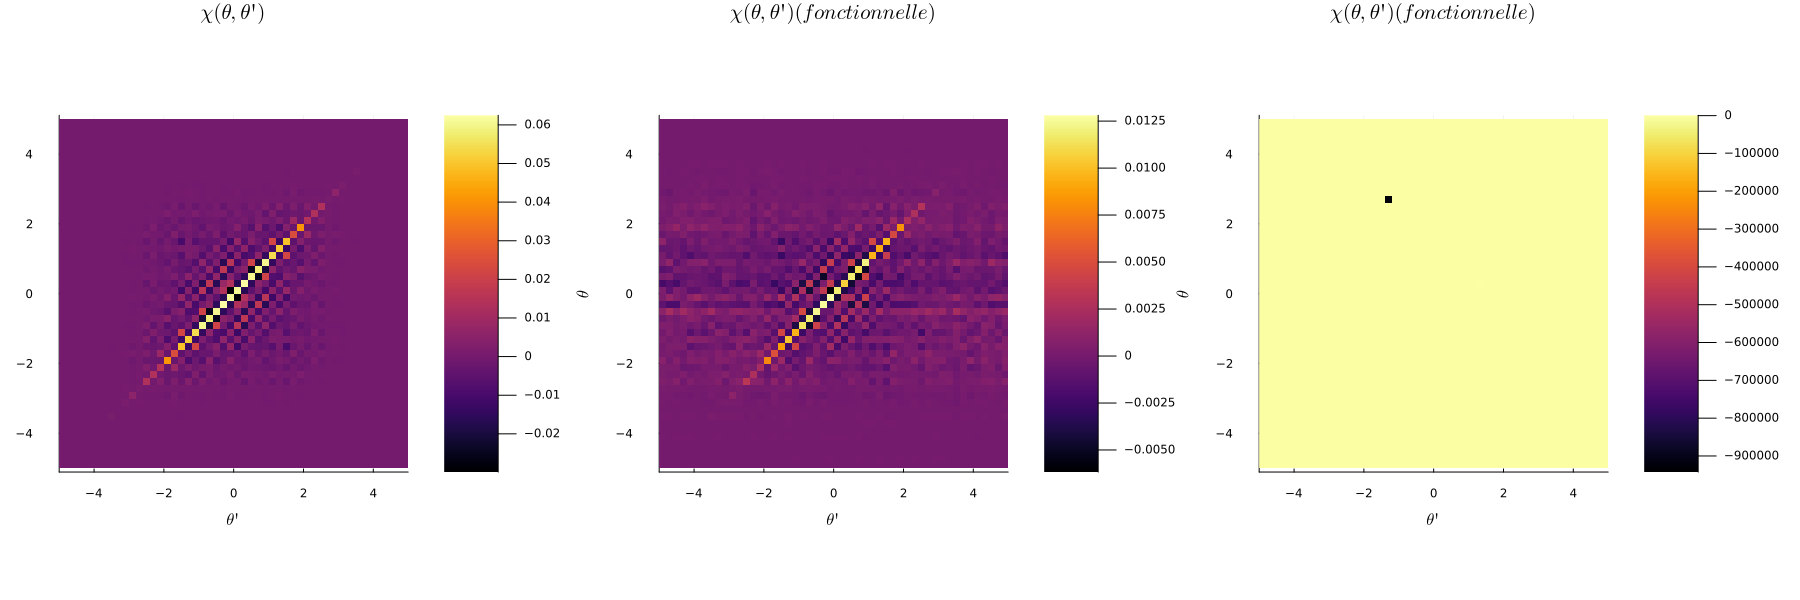
\includegraphics[width=1\textwidth]{figures/04_GGE_Fluctuation/figure_fluctuations}
    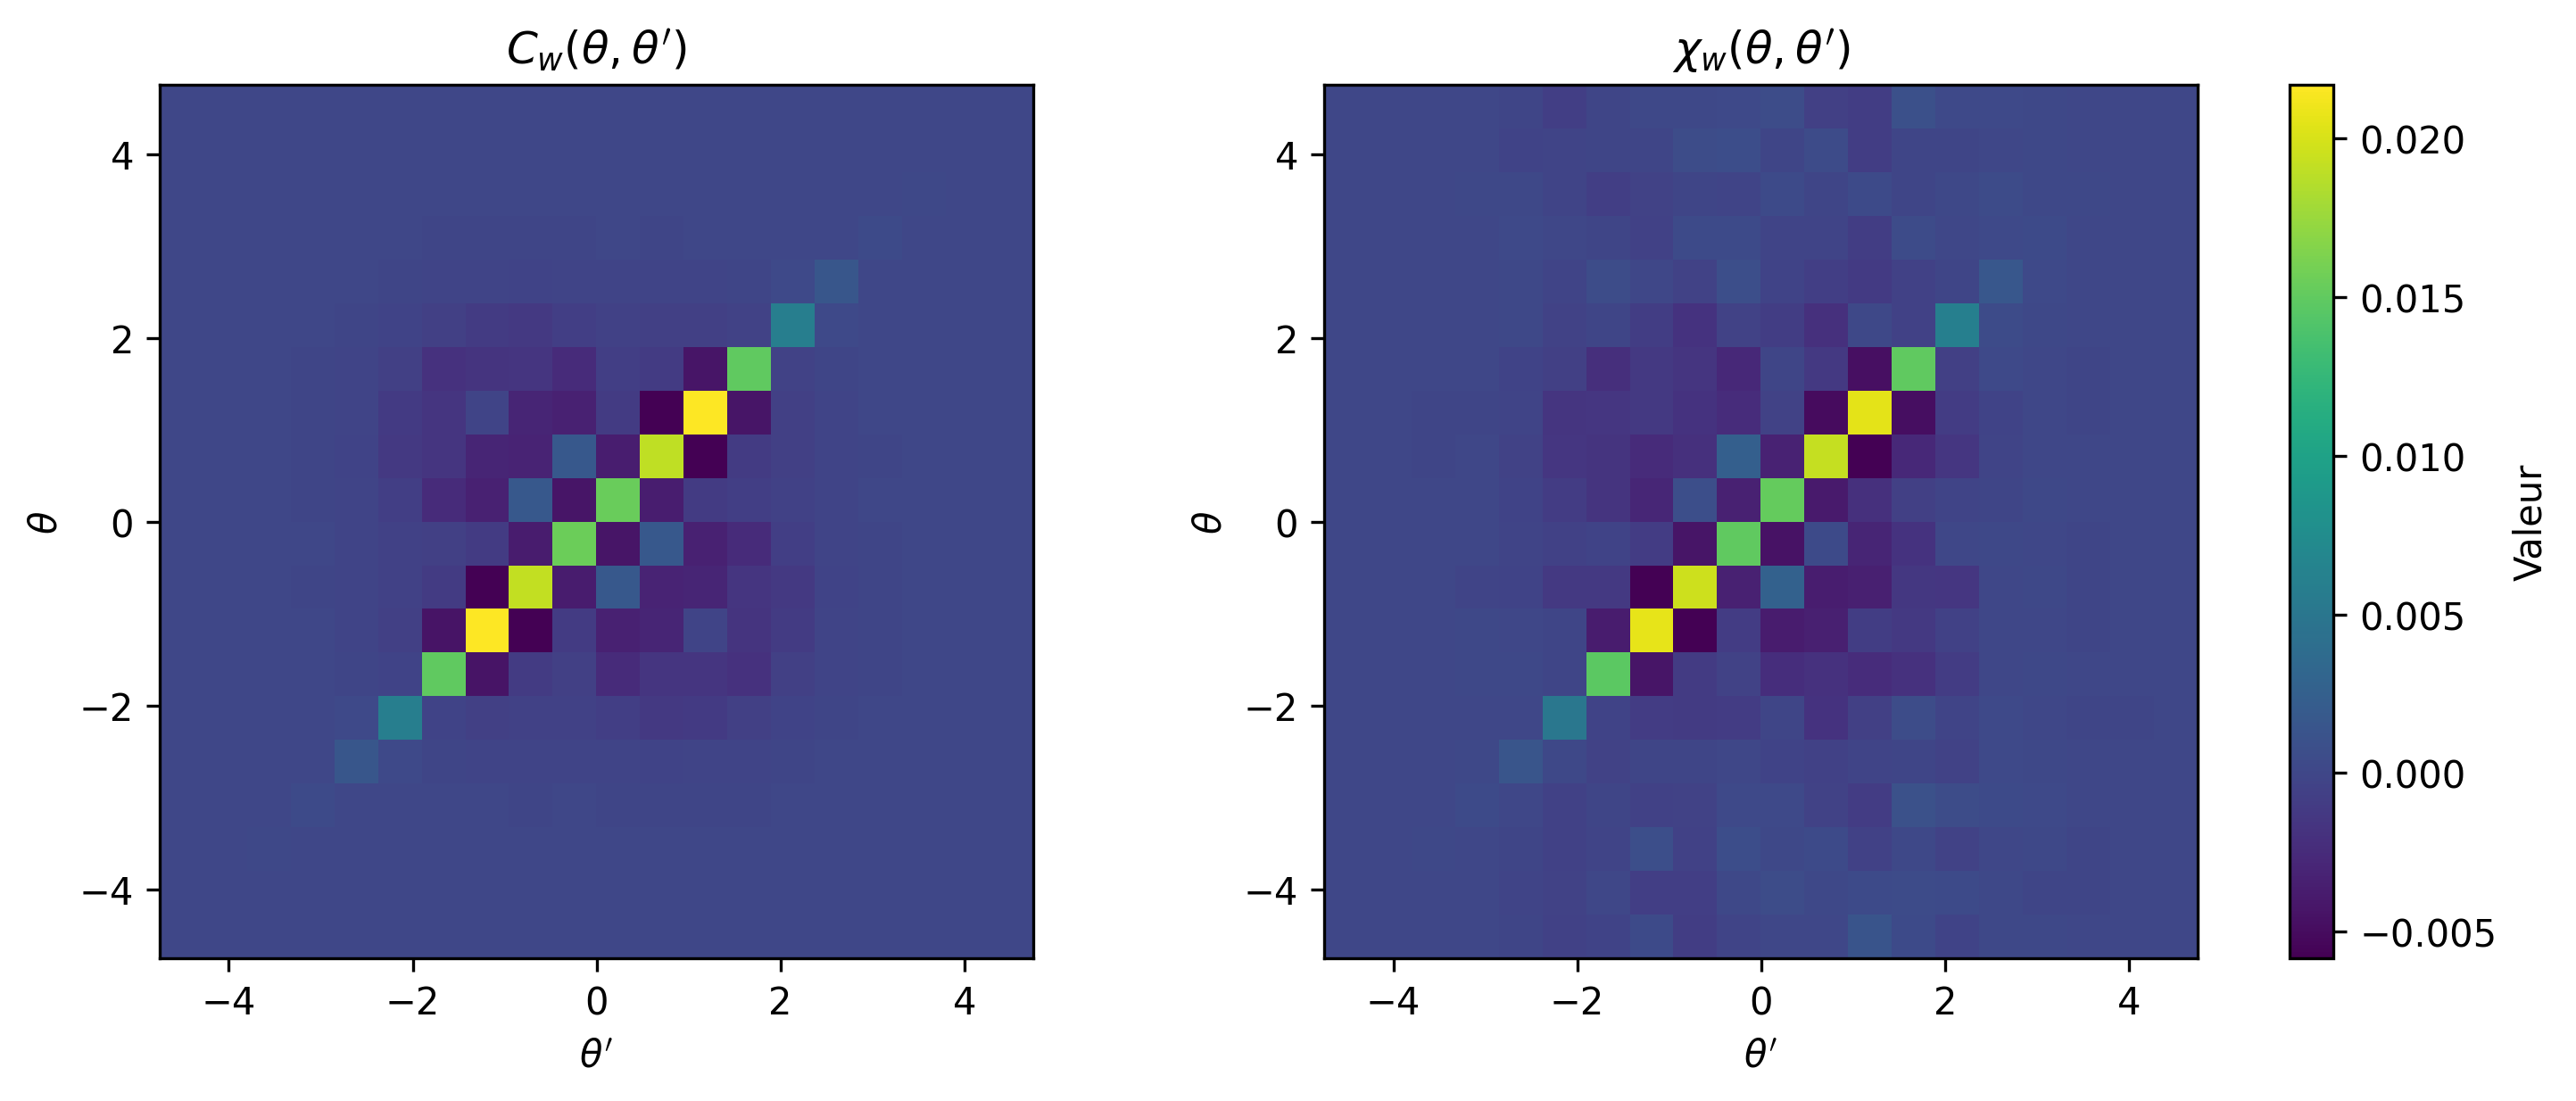
\includegraphics[width=1\textwidth]{figures/04_GGE_Fluctuation/heatmaps.png}
    \caption{Comparaison des matrices pour $\braket{\operator{\rho}(\theta)\operator{\rho}(\theta')}_w$ : à gauche la corrélation  \( C_w(\theta,\theta') \) ; à droite la susceptibilité \( \chi_w(\theta,\theta') \) obtenue par dérivée fonctionnelle pour \( N_{\rm conf} = 2 \times 10^6 \) et \( \varepsilon = 10^{-1} \).}
    \label{fig:comparison_chi_C}
\end{figure}

\paragraph{Discussion.}

Les figures montrent une concordance satisfaisante entre les deux matrices. L’écart relatif est d’environ 13,5\,\%, et provient principalement des erreurs statistiques liées à la méthode \emph{Monte Carlo} et de l’approximation par différences finies dans le calcul de la dérivée fonctionnelle.

\medskip

Le principe de fluctuation-réponse dans le cadre du \gls{GGE} étant supposé valide, l’objectif de cette analyse n’est pas de le confirmer, mais de vérifier que l’on reste en capacité d’échantillonner correctement les fluctuations à partir de \(\chi_w(\theta,\theta')\) avec un nombre fini de configurations. L’erreur relative observée est donc acceptable et reflète les limites statistiques de l’expérience numérique.

\medskip

La précision peut être améliorée en augmentant le nombre de configurations \(N_{\rm conf}\) :

% \begin{itemize}[label = $\bullet$]
% 	\item Le calcul de \(C_w(\theta, \theta')\) est en \(\mathcal{O}(N_{\rm conf})\) et celui de \(\chi_w(\theta, \theta')\) en \(\mathcal{O}(N_{\rm conf} \cdot N_{\rm cell})\), où \(N_{\rm cell}\) est le nombre de points de la grille en \(\theta\).
% 	\item Pour \(N_{\rm conf} = 2\times 10^6\) et \(N_{\rm cell} = 20\), la matrice \(C_w(\theta, \theta')\) se calcule en environ 6 minutes et \(\chi_w(\theta, \theta')\) en environ 2 heures.
% 	\item On peut envisager \(N_{\rm conf} = 10^7\) : \(C_w(\theta, \theta')\) en 30 minutes et \(\chi_w(\theta, \theta')\) en 10 heures.
% \end{itemize}

\begin{itemize}[label = $\bullet$]
    \item Dans ce point, les symboles de Landau \(\mathcal{O}(\cdot)\) désignent ici des \emph{complexités en temps de calcul}. 
    Le calcul de la matrice de corrélation \(C_w(\theta, \theta')\) s'effectue en un temps 
    de complexité \(\mathcal{O}(N_{\rm conf})\), tandis que celui de la susceptibilité 
    \(\chi_w(\theta, \theta')\) nécessite un temps de complexité 
    \(\mathcal{O}(N_{\rm conf} \cdot N_{\rm cell})\), où \(N_{\rm cell}\) est le nombre de points 
    de discrétisation de la variable \(\theta\).

    \item Pour un nombre de configurations\emph{Monte Carlo} fixé à 
    \(N_{\rm conf} = 2 \times 10^6\) et une grille de taille \(N_{\rm cell} = 20\), 
    on obtient un temps de calcul d'environ 6 minutes pour la matrice \(C_w(\theta,\theta')\), 
    tandis que le calcul de \(\chi_w(\theta,\theta')\), plus coûteux car nécessitant 
    l'évaluation d'une réponse à une perturbation sur chaque cellule, demande environ 2 heures.

    \item Si l'on augmente le nombre de configurations à 
    \(N_{\rm conf} = 10^7\), ce qui permet de réduire plus fortement le bruit statistique, 
    alors le calcul de \(C_w(\theta,\theta')\) prendrait environ 30 minutes, 
    tandis que celui de \(\chi_w(\theta,\theta')\) nécessiterait approximativement 10 heures, 
    en raison du facteur multiplicatif supplémentaire lié à la grille 
    \(\theta \mapsto \theta_i\).
\end{itemize}


\medskip

Pour de petits \(N_{\rm conf}\), la perturbation \(\varepsilon\) doit être augmentée pour que les fluctuations calculées ne soient pas noyées dans le bruit. Si \(\varepsilon\) est trop grand, on observe toujours la structure globale de \(\chi_w(\theta, \theta')\), mais avec une amplitude réduite :
\begin{eqnarray*}
	\chi_w(\theta, \theta') \approx \alpha C_w(\theta, \theta'), \quad 0 < \alpha < 1.
\end{eqnarray*}

Par exemple, pour \(N_{\rm conf} = 10^5\), la mesure \eqref{cha4:eq:std.1} est de $8\%$.  On peut utiliser \(N_{\rm cell} = 100\) et \(\varepsilon = 1\), et obtenir :
\begin{eqnarray*}
    \frac{\left\Vert  \alpha C_w - \chi_w \right\Vert_2}{\left\Vert \alpha C_w \right\Vert_2} \;\sim\; 27\%
\end{eqnarray*}
avec $\alpha = 0.078$ et pour un temps de calcul de $26~min$ (Fig~\ref{fig:comparison_chi_C_1}).
\begin{figure}[H]
    \centering
    %\includegraphics[width=0.32\textwidth]{chi_matrix.png}
    %\includegraphics[width=0.32\textwidth]{C_matrix.png}
    %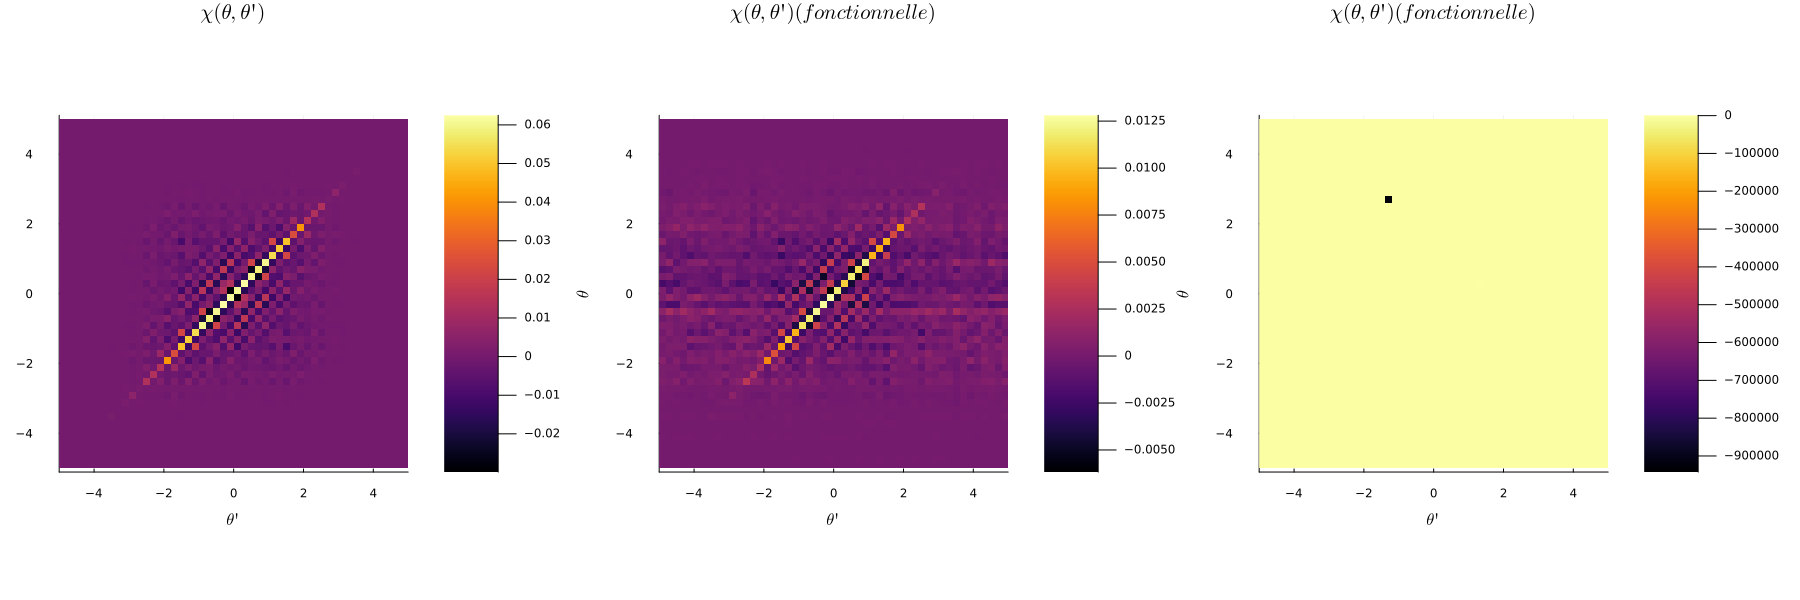
\includegraphics[width=1\textwidth]{figures/04_GGE_Fluctuation/figure_fluctuations}
    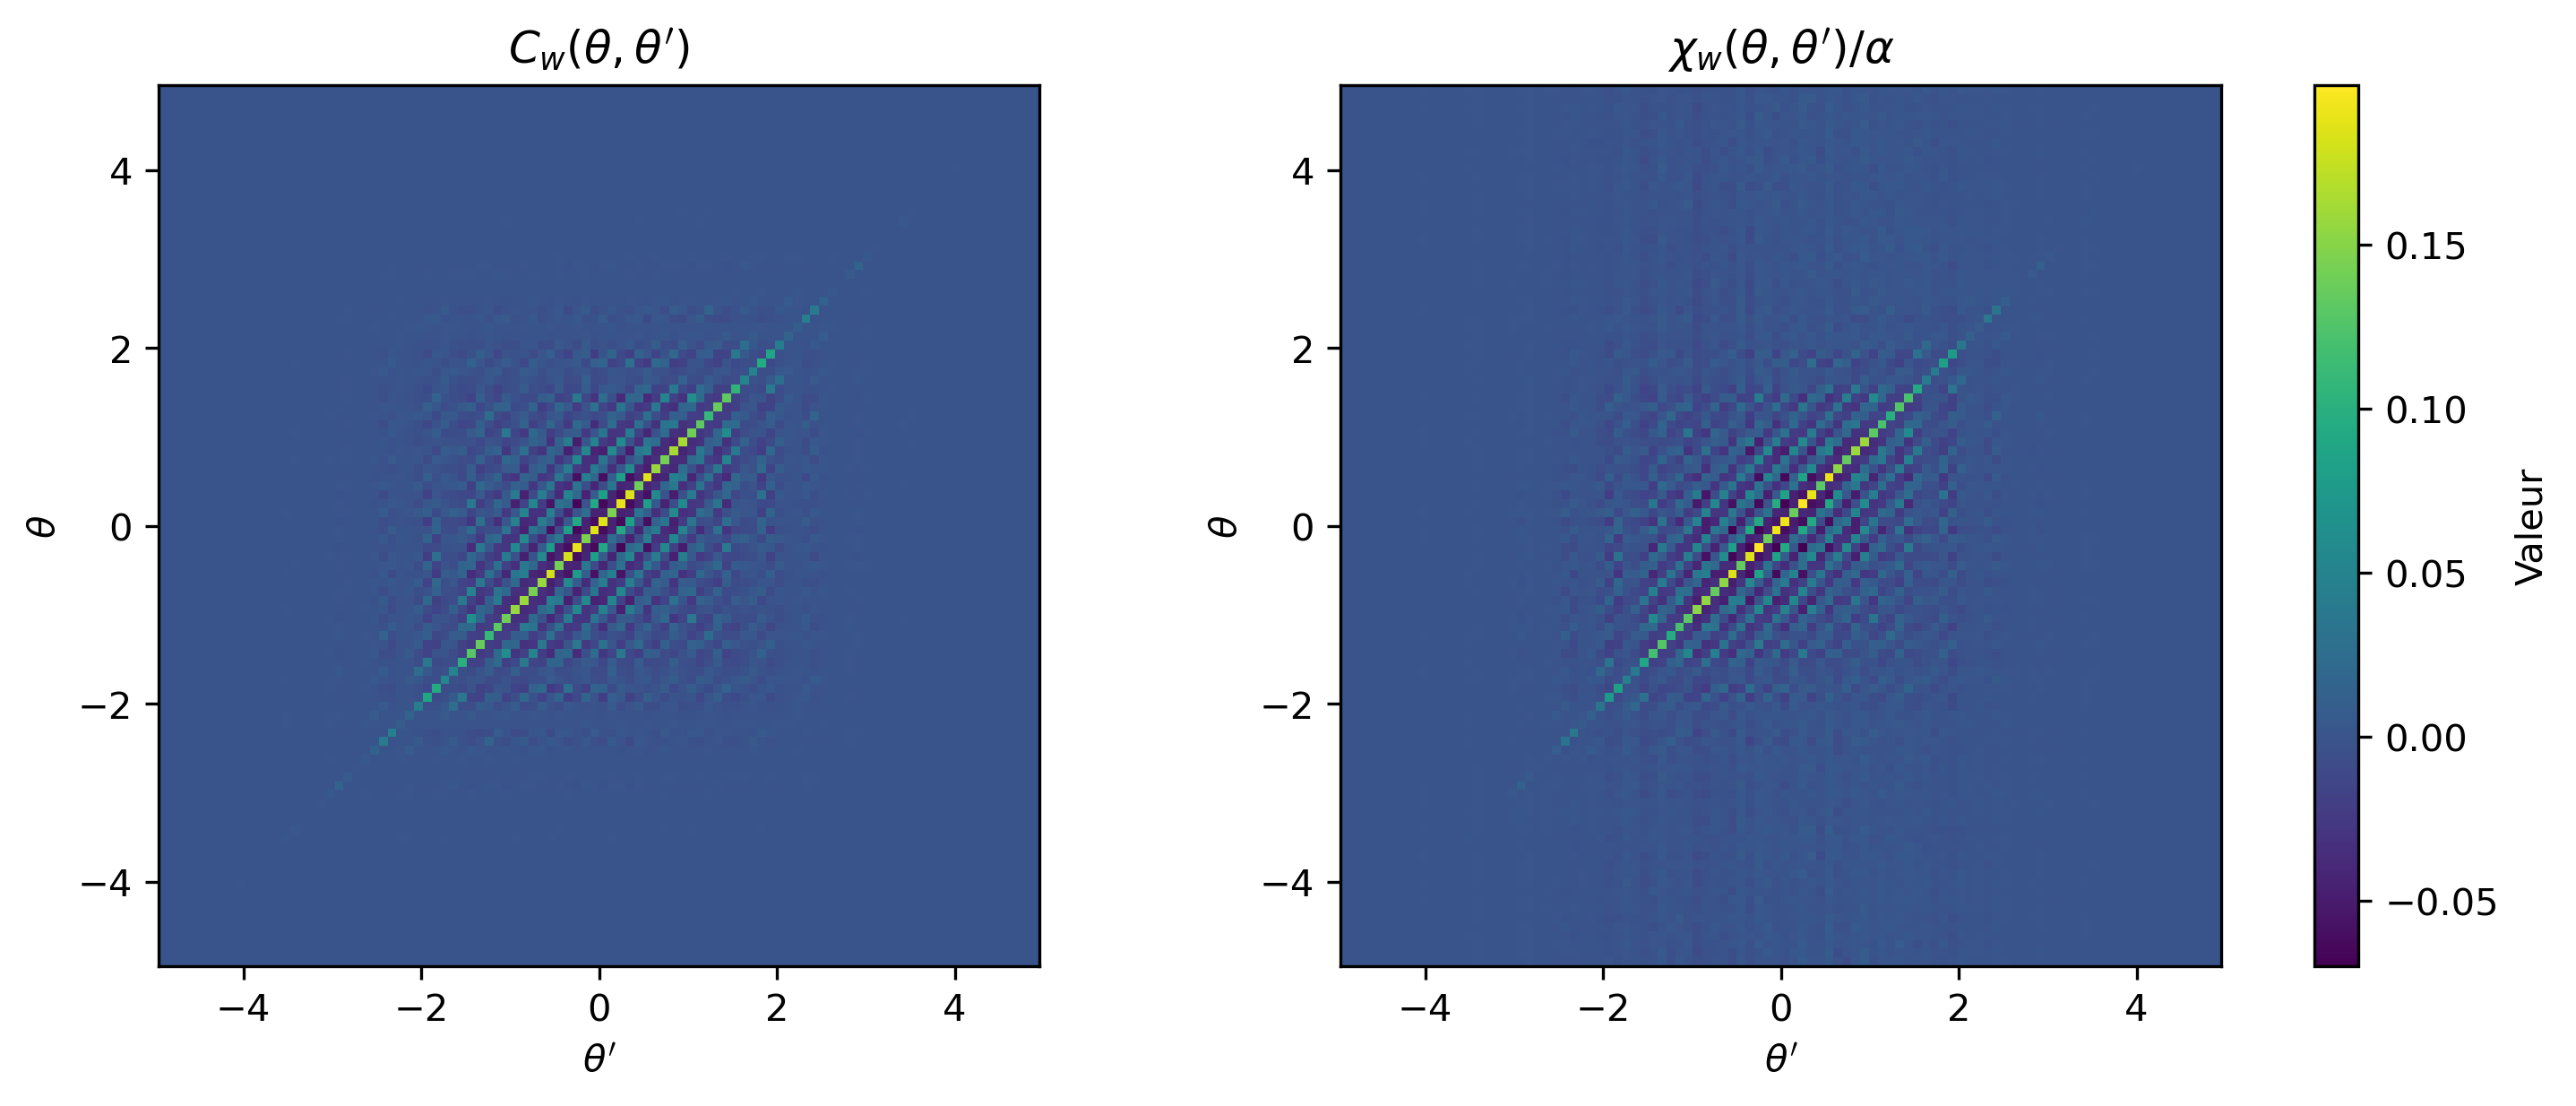
\includegraphics[width=1\textwidth]{figures/04_GGE_Fluctuation/heatmaps_1.png}
    \caption{Comparaison des matrices pour $\braket{\operator{\rho}(\theta)\operator{\rho}(\theta')}_w$ : à gauche la corrélation  \( C_w(\theta,\theta') \) ; à droite la susceptibilité \( \chi_w(\theta,\theta')/\alpha \) obtenue par dérivée fonctionnelle, pour  \(N_{\rm cell} = 100\), \(\varepsilon = 1\) et \(\alpha = 0.078\).}
    \label{fig:comparison_chi_C_1}
\end{figure}

Physiquement, \(\alpha < 1\) reflète le fait que pour un nombre limité de configurations, la réponse calculée par différences finies sous-estime légèrement l’amplitude des fluctuations par rapport à la covariance brute \(C_w\), mais la structure globale reste correcte. En augmentant \(N_{\rm conf}\), \(\alpha \to 1\) et \(\chi_w(\theta, \theta')\) converge vers \(C_w(\theta, \theta')\) dans la limite des grandes statistiques.




%On a vus dans l'equation ~\eqref{??} que pour une fonction teste quelquonque , $f \colon \mathbb{R} \to \mathbb{R}$, $\operator{\mathcal{Q}}[f]$ s'écrit de la forme integrale
%
%
%Nous avons vu que l'espérance d'une charge généralisée \( \operator{\mathcal{Q}}[f_1] \) dans cet état, notée au chapitre~(\ref{chap:relaxation}) \( \langle \operator{\mathcal{Q}}^{(\mathcal{S})}[f_1] \rangle_{\operator{\rho}_{\mathrm{GGE}}^{(\mathcal{S})}[w]} \), peut être simplifiée, dans ce chapitre, en :
%\begin{eqnarray*}
%	\langle \operator{\mathcal{Q}}[f_1] \rangle_w =  -  \left . \frac{ \delta \ln Z [w] }{ \delta f_1  } \right)_{w}  = \mathrm{Tr} \left[ \operator{\rho}_{\mathrm{GGE}}[w]\, \operator{\mathcal{Q}}[f_1] \right]
%= \frac{1}{Z[w]}\, \mathrm{Tr} \left[ e^{-\operator{\mathcal{Q}}[w]}\, \operator{\mathcal{Q}}[f_1] \right] .
%\end{eqnarray*}
%
%Par souci de lisibilité, nous omettrons les indices \((\mathcal{S})\) : le caractère local des observables étant désormais implicite.
%
%
%
%%On a vus  que l’espérance d’une observable $\operator{\mathcal{Q}}^{(\mathcal{S})}[f_1]$ dans le GGE , noté dans le chapitre \ref{} par $\langle \operator{\mathcal{Q}}^{(\mathcal{S})}[f_1] \rangle_{\operator{\rho}_{\mathrm{GGE}}^{(\mathcal{S})}[w]}$ que pour soucis d'aléger dans lé résonement on notéra $\langle \operator{\mathcal{Q}}[f_1] \rangle$, et j'enlève les $(\mathcal{S})$, le caractère locale étant maintenat inplicite , est donnée par :
%
%\medskip
%
%%La dérivée fonctionnelle de l'espérance de la charge $\operator{\mathcal{Q}}[f_1]$ par rapport au potentiel conjugué $f_2$ est donnée par :
%La dérivée fonctionnelle de l'espérance de \( \operator{\mathcal{Q}}[f_1] \) par rapport à une autre fonction test \( f_2 \), représentant un potentiel conjugué, donne la réponse linéaire croisée :
%
%\begin{eqnarray*}
%	\chi_w[f_1, f_2] \doteq   \left . \frac{ \delta^2 \ln Z [w] }{ \delta f_1 \delta f_2 } \right)_{w} =  - \left.\frac{\delta \langle \operator{\mathcal{Q}}[f_1] \rangle}{\delta f_2} \right )_w = C_w[f_1, f_2] ,
%\end{eqnarray*}
%
%avec le fonction corrélation à deux points :
%
%\begin{eqnarray*}
%	C_w[f_1, f_2] \doteq  	\langle ( \operator{\mathcal{Q}}[f_1] - \langle \operator{\mathcal{Q}}[f_1] \rangle_w ) ( \operator{\mathcal{Q}}[f_2] - \langle \operator{\mathcal{Q}}[f_f] \rangle_w  ) \rangle_w = \langle \operator{\mathcal{Q}}[f_1] \operator{\mathcal{Q}}[f_2] \rangle_w - \langle \operator{\mathcal{Q}}[f_1] \rangle_w \langle \operator{\mathcal{Q}}[f_2] \rangle_w.
%\end{eqnarray*}
%
%
%Autrement dit, la dérivée fonctionnelle seconde du logarithme de la fonction de partition fournit la covariance des charges \( \operator{\mathcal{Q}}[f_1] \) et \( \operator{\mathcal{Q}}[f_2] \), illustrant le principe de fluctuation-réponse dans ce contexte diagonal.
%
%\paragraph{Démonstration.}
%
%Pour établir le lien entre réponse linéaire et fluctuations, nous allons partir de l'expression intégrale des charges généralisées, puis montrer que la susceptibilité associée correspond bien à la fonction de corrélation des fluctuations de densité de rapidité.
%
%
%\subparagraph{Charge généralisé sous forme intégrale.}
%Pour le démontrer on écrit la charge généralisé sous forme intégrale :
%\begin{eqnarray*}
%\operator{\mathcal{Q}}[f] = L\int d\theta f(\theta) \operator{\rho}(\theta)
%\end{eqnarray*}
%où $\operator{\rho}(\theta)$ est l'opérateur densité spectal , agissant comme :
%\(
%\operator{\rho}(\theta) \ket{ \{ \theta_a \} } = \frac{1}{L} \sum \delta ( \theta - \theta_a ) \ket{ \{ \theta_a \} }.
%\)
%
%\subparagraph{Dérivée fonctionnelle.}
%On dérive cette expression par rapport à $w_2$. En utilisant la dérivée d’un rapport :
%\(
%	\left.\frac{\delta}{\delta f_2} \left( \frac{A[w]}{Z[w]} \right) \right |_{w} = \frac{1}{Z[w]}\, \left.\frac{\delta A[w]}{\delta f_2} \right|_{w} - \frac{A[w]}{Z[w]^2}\, \left.\frac{\delta Z[w]}{\delta f_2}\right|_{w} ,
%\)
%avec $A[w] \equiv \mathrm{Tr}[e^{-\operator{\mathcal{Q}}[w]} \operator{\mathcal{Q}}[f_1]]$, on obtient :
%\begin{eqnarray*}
%	\left . \frac{\delta \langle \operator{\mathcal{Q}}[f_1] \rangle_w}{\delta f_2} \right )_w
%	= \frac{1}{Z[w]}\, \frac{\delta A[w]}{\delta f_2}
%	- \langle \operator{\mathcal{Q}}[f_1] \rangle_w \cdot \frac{1}{Z[w]}\, \frac{\delta Z[w]}{\delta f_2}.
%\end{eqnarray*}
%
%\subparagraph{Dérivées explicites.}
%Utilisons la propriété démontrée précédemment :
%\(
%	\frac{\delta \operator{\mathcal{Q}}[w]}{\delta f_2} = \operator{\mathcal{Q}}[f_2]	.
%\)
%En notant que la dérivée d’une exponentielle diagonale est simple :
%\(
%\frac{\delta}{\delta f_2} e^{-\operator{\mathcal{Q}}[w]} = - \operator{\mathcal{Q}}[f_2]\, e^{-\operator{\mathcal{Q}}[w]},
%\)
%on obtient :
%\begin{eqnarray*}
%\frac{\delta A[w]}{\delta f_2} = - \mathrm{Tr}\left[ \operator{\mathcal{Q}}[f_2]\, e^{-\operator{\mathcal{Q}}[w]} \operator{\mathcal{Q}}[f_1] \right],
%\quad
%\frac{\delta Z[w]}{\delta f_2} = - \mathrm{Tr}\left[ \operator{\mathcal{Q}}[f_2]\, e^{-\operator{\mathcal{Q}}[w]} \right].
%\end{eqnarray*}
%
%\subparagraph{Regroupement.}
%En regroupant les termes, on trouve :
%\begin{eqnarray*}
%	\chi_w[f_1, f_2]&  \doteq & - \left.\frac{\delta \langle \operator{\mathcal{Q}}[f_1] \rangle_w}{\delta f_2} \right )_w  \\
%&=& \frac{1}{Z[w]}\, \mathrm{Tr}\left[ \operator{\mathcal{Q}}[w_2]\, e^{-\operator{\mathcal{Q}}[w]}\, \operator{\mathcal{Q}}[f_1] \right]
%- \langle \operator{\mathcal{Q}}[f_1] \rangle_w \cdot \frac{1}{Z[w]}\, \mathrm{Tr}\left[ \operator{\mathcal{Q}}[f_2]\, e^{-\operator{\mathcal{Q}}[w]} \right] \\
%&=& \langle \operator{\mathcal{Q}}[f_2]\, \operator{\mathcal{Q}}[f_1] \rangle_w - \langle \operator{\mathcal{Q}}[f_1] \rangle_w\, \langle \operator{\mathcal{Q}}[f_2] \rangle_w.
%\end{eqnarray*}
%
%\medskip
%
%\subparagraph{Conclusion.} Dans un état diagonal tel que le GGE, la susceptibilité est égale à la covariance entre charges généralisées, illustrant le principe de \emph{fluctuation-réponse}.
%%\paragraph{Remarques.}
%La matrice $\chi_w[f_1, f_2]$ s’interprète donc comme la covariance de la densité spectrale projetée sur les fonctions test $f_1$ et $f_2$.
%Un cas particulier d’intérêt est la susceptibilité d’une seule charge :
%\begin{eqnarray*}
%\chi_w[f] \equiv \chi_w[f, f] = \mathrm{Var}_w(\operator{\mathcal{Q}}[f]) = \langle \operator{\mathcal{Q}}[f]^2 \rangle_w - \langle \operator{\mathcal{Q}}[f] \rangle_w^2
%= L^2 \iint d\theta\, d\theta'\, f(\theta)\, C_w(\theta, \theta')\, f(\theta').
%\end{eqnarray*}
%
%
%\subsection{Corrélations spectrales et susceptibilité}
%
%%\paragraph{Corrélations spectrales et susceptibilité.}
%
%La susceptibilité fonctionnelle peut s’exprimer, dans la base des fonctions test, comme une forme bilinéaire projetée sur la fonction de corrélation spectrale :
%\begin{eqnarray*}
%\chi_w[f_1, f_2] = C_w[f_1, f_2] = L^2 \iint d\theta\, d\theta'\, f_1(\theta)\, C_w(\theta, \theta')\, f_2(\theta'),
%\end{eqnarray*}
%où la fonction de corrélation spectrale \( C_w(\theta, \theta') \) est définie comme la covariance des fluctuations de densité spectrale :
%\begin{eqnarray*}
%C_w(\theta, \theta') \doteq \langle \delta \operator{\rho}(\theta)\, \delta \operator{\rho}(\theta') \rangle_w = \langle \operator{\rho}(\theta)\, \operator{\rho}(\theta') \rangle_w - \langle \operator{\rho}(\theta) \rangle_w\, \langle \operator{\rho}(\theta') \rangle_w.
%\end{eqnarray*}
%
%Par ailleurs, l’espérance de la densité spectrale s’obtient comme une dérivée fonctionnelle du logarithme de la fonction de partition :
%\begin{eqnarray*}
%\langle \operator{\rho}(\theta) \rangle_w = - \frac{1}{L} \left. \frac{\delta \ln Z[w]}{\delta w(\theta)} \right),
%\end{eqnarray*}
%et la susceptibilité spectrale, définie comme la réponse de \( \langle \rho(\theta) \rangle_w \) à une variation de \( w(\theta') \), s’écrit :
%\begin{eqnarray*}
%\chi_w(\theta, \theta') = \left. \frac{1}{L^2} \frac{\delta^2 \ln Z[w]}{\delta w(\theta)\, \delta w(\theta')} \right) = - \left. \frac{1}{L} \frac{\delta \langle \operator{\rho}(\theta) \rangle_w}{\delta w(\theta')} \right).
%\end{eqnarray*}
%
%Ainsi, dans l’état diagonal \( \operator{\rho}_{\mathrm{GGE}}[w] \), la susceptibilité spectrale coïncide avec la fonction de corrélation \( C_w(\theta, \theta') \), illustrant le principe de \emph{fluctuation-réponse}.
%



\section{Limite thermodynamique, structure variationnelle et susceptibilité}

\subsection{Susceptibilité spectrale et structure variationnelle de l’entropie}

\begin{mdframed}[
	linewidth=0.5pt,
	backgroundcolor=gray!5,
	roundcorner=50pt,
	innerleftmargin=5pt,
    innerrightmargin=5pt,
    innertopmargin=-10pt,
    innerbottommargin=2pt,
    leftmargin=2pt,
    rightmargin=2pt
	]
\paragraph{Rappel : Approche thermodynamique (Yang–Yang et énergie généralisée).}

Dans l’approximation thermodynamique, le sous-système est décrit en termes de grandeurs macroscopiques, notamment par la distribution de rapidité $\rho(\theta)$.
Dans l’équation \eqref{chap:TBA:eq:ensemble_average}, nous avons vu que, dans la limite thermodynamique, la moyenne d’une observable s’écrit :
\begin{eqnarray}
	\langle \operator{\mathcal{O}} \rangle_{w} & = & \frac{\int \mathcal{D} \rho \; e^{L (\mathcal{S}_{YY}[\rho] - \mathcal{W}[\rho])} \, \langle\operator{\mathcal{O}}\rangle_{[\rho]}}{\int \mathcal{D} \rho \; e^{L (\mathcal{S}_{\mathrm{YY}}[\rho] - \mathcal{W}[\rho])}}. \label{chap:Fluc:eq:ensemble_average}
\end{eqnarray}
où $\mathcal{S}_{\mathrm{YY}}$ est l’entropie de \gls{YY} et $\mathcal{W}$ l’énergie généralisée, introduites respectivement dans \eqref{chap.2.entropi.int} et \eqref{chap.2.W.int}, que l'on rappelle.
\begin{eqnarray}
	\mathcal{S}_{YY}[\rho] & = & \int d \theta  \, [ \rho_s\ln \rho_s - \rho \ln \rho - ( \rho_s - \rho ) \ln ( \rho_s - \rho ) ] (\theta) , \label{chap.4.entropi.int}\\
	\mathcal{W}[\rho] & = & \int   w(\theta) \rho(\theta) \, d \theta, \label{chap.4.W.int}
\end{eqnarray}
où \(\rho_s(\theta)\) désigne la {\em densité d’états} liée à \(\rho\) par les équations de \gls{BA} \eqref{eq:TBA-rhos} :
\begin{eqnarray}
	2\pi \rho_s = 1 + \Delta \star \rho.
\end{eqnarray}

\medskip

La quantité $\langle\operator{\mathcal{O}}\rangle_{[\rho]}$ désigne la valeur propre de l’observable associée aux états caractérisés par la distribution de rapidité $\rho$.




\end{mdframed}

\medskip

\begin{mdframed}[
	linewidth=0.5pt,
	backgroundcolor=gray!5,
	roundcorner=50pt,
	innerleftmargin=5pt,
    innerrightmargin=5pt,
    innertopmargin=-10pt,
    innerbottommargin=2pt,
    leftmargin=2pt,
    rightmargin=2pt
]
\paragraph{Rappel : Condition variationnelle du GGE.}


À l’équilibre thermodynamique; dans la limite $L \to \infty$, la distribution $\rho_{\mathrm{eq}}(\theta)$ satisfait l’équation \eqref{chap.2:eq.rho.eq.1}, et coïncide alors avec la moyenne de l’opérateur de densité de rapidité :
\begin{eqnarray}
	 \rho_{\mathrm{eq}}(\theta) =  \braket{ \operator{\rho}(\theta) }_w,
\end{eqnarray}
représentant ainsi la densité continue de quasi-particules dans l’état stationnaire / d’équilibre.


\medskip

Dans le cadre du \gls{GGE} continu, l’état macroscopique est entièrement déterminé par la densité spectrale $\rho(\theta)$ qui maximise l’entropie de \acrlong{YY}, $\mathcal{S}_{\mathrm{YY}}[\rho]$, sous la contrainte de conservation des charges généralisées. Le poids spectral $w(\theta)$ est alors fixé.
Comme nous l’avons vu (au chapitre~(\ref{chap:relaxation})), la condition d’équilibre \eqref{chap:TBA:eq:stationnarite-3} peut s’écrire sous la forme variationnelle :
\begin{eqnarray}
	\left. \frac{\delta \mathcal{S}_{\mathrm{YY}}[\rho]}{\delta \rho(\theta)} \right)_{\rho = \rho_{\mathrm{eq}}} = w(\theta). \label{chap:Fluc:eq:stationnarite-3}
\end{eqnarray}

\end{mdframed}

%\begin{mdframed}[
%	linewidth=0.5pt,
%	backgroundcolor=gray!5,
%	roundcorner=50pt,
%	innerleftmargin=5pt,
%    innerrightmargin=5pt,
%    innertopmargin=-10pt,
%    innerbottommargin=2pt,
%    leftmargin=2pt,
%    rightmargin=2pt
%]
%\paragraph{Rappel : Approche thermodynamique (\gls{YY} et énergie généralisée).}
%
%Dans l’approximation thermodynamique, le système est décrit en termes de grandeurs macroscopiques, notamment par la distribution de rapidité $\rho(\theta)$.
%Dans l’équation \eqref{chap:TBA:eq:ensemble_average}, la moyenne d’un observable s’écrit, dans la limite thermodynamique :
%\begin{eqnarray}
%	\langle \operator{\mathcal{O}} \rangle_{w} & = &
%	\frac{\int \mathcal{D} \rho \; e^{L (\mathcal{S}_{YY}[\rho] - \mathcal{W}[\rho])} \,
%	\langle\operator{\mathcal{O}}\rangle_{[\rho]}}
%	{\int \mathcal{D} \rho \; e^{L (\mathcal{S}_{\mathrm{YY}}[\rho] - \mathcal{W}[\rho])}}.
%	\label{chap:Fluc:eq:ensemble_average}
%\end{eqnarray}
%où $\mathcal{S}_{\mathrm{YY}}$ est l’entropie de \gls{YY} et $\mathcal{W}$ l’énergie généralisée :
%\begin{eqnarray}
%	\mathcal{S}_{YY}[\rho] & = & \int d \theta
%	\big[ \rho_s\ln \rho_s - \rho \ln \rho - ( \rho_s - \rho ) \ln ( \rho_s - \rho ) \big] (\theta),
%	\label{chap.4.entropi.int}\\
%	\mathcal{W}[\rho] & = & \int   w(\theta) \rho(\theta) \, d \theta,
%	\label{chap.4.W.int}
%\end{eqnarray}
%avec $\rho_s(\theta)$ la densité d’états reliée à $\rho$ par les équations de \gls{BA} \eqref{eq:TBA-rhos} :
%\begin{eqnarray}
%	2\pi \rho_s = 1 + \Delta \star \rho.
%\end{eqnarray}
%\end{mdframed}
%
%\begin{mdframed}[
%	linewidth=0.5pt,
%	backgroundcolor=gray!5,
%	roundcorner=50pt,
%	innerleftmargin=5pt,
%    innerrightmargin=5pt,
%    innertopmargin=-10pt,
%    innerbottommargin=2pt,
%    leftmargin=2pt,
%    rightmargin=2pt
%]
%\paragraph{Rappel : Condition variationnelle du GGE.}
%
%À l’équilibre thermodynamique, la distribution $\rho_{\mathrm{eq}}(\theta)$ coïncide avec la moyenne de l’opérateur de densité de rapidité :
%\begin{eqnarray}
%	 \rho_{\mathrm{eq}} =  \braket{ \operator{\rho}(\theta) }_w.
%\end{eqnarray}
%
%Dans le cadre du GGE continu, l’état macroscopique est entièrement déterminé par une densité spectrale $\rho(\theta)$ qui maximise l’entropie de \gls{YY}, $\mathcal{S}_{\mathrm{YY}}[\rho]$, sous contrainte des charges généralisées. Le poids spectral $w(\theta)$ est alors fixé.
%
%La condition d’équilibre peut s’écrire sous forme variationnelle :
%\begin{eqnarray}
%	\left. \frac{\delta \mathcal{S}_{\mathrm{YY}}[\rho]}{\delta \rho(\theta)} \right|_{\rho = \rho_{\mathrm{eq}}}
%	= w(\theta).
%	\label{chap:Fluc:eq:stationnarite-3}
%\end{eqnarray}
%\end{mdframed}
%


\medskip
\paragraph{Dérivée fonctionnelle.}
On peut considérer l’équation d’équilibre comme une relation implicite définissant le poids spectral $w$ comme une fonctionnelle de la distribution de rapidité $\rho$. La dérivée fonctionnelle de cette relation s’écrit :
\begin{eqnarray}
	\left. \frac{\delta w(\theta)}{\delta \rho(\theta')} \right)_{\rho = \rho_{\mathrm{eq}}} = \left. \frac{\delta^2 \mathcal{S}_{\mathrm{YY}}[\rho]}{\delta \rho(\theta)\, \delta \rho(\theta')} \right)_{\rho = \rho_{\mathrm{eq}}}, \label{chap:Fluc:eq:susp-1}
\end{eqnarray}
où le membre de droite représente l’opérateur hessien (ou courbure fonctionnelle) de l'entropie de \gls{YY}, évalué à l’équilibre. Cet opérateur est défini négatif, conformément à l’interprétation de $\mathcal{S}_{\mathrm{YY}}$ comme une entropie à maximiser.

\paragraph{Inversion.}
On en déduit que la réponse de $\rho$ à une variation infinitésimale du poids spectral $w$ est donnée par l'inverse fonctionnel de \eqref{chap:Fluc:eq:susp-1} :
\begin{eqnarray}
	-\frac{1}{L} \left. \frac{\delta \rho(\theta)}{\delta w(\theta')} \right)_{\rho = \rho_{\mathrm{eq}}} = - \left( L \left. \frac{\delta^2 \mathcal{S}_{\mathrm{YY}}[\rho]}{\delta \rho(\theta)\, \delta \rho(\theta')} \right)_{\rho = \rho_{\mathrm{eq}}} \right)^{-1}. \label{chap:Fluc:eq:susp-2}
\end{eqnarray}
La susceptibilité fonctionnelle $\chi_w(\theta, \theta')$, définie dans \eqref{chap4:eq.susceptibilite-fonctionnelle_3}, coïncide avec cette expression.


\subsection{Fluctuations gaussiennes autour de l’équilibre thermodynamique}

Une autre approche pour accéder aux fluctuations de la distribution de rapidité $\rho = \rho_{\mathrm{eq}} + \delta \rho $  est d'étudier la structure variationnelle de l’action effective $\mathcal{S}_{YY} - \mathcal{W}$ autour du point d’équilibre $\rho_{\mathrm{eq}}$. En effet, par définition de ce point d’équilibre, toute variation infinitésimale $\delta \rho$ satisfait  \cite{Wheeler_FieldTheory_Ch5}:
\begin{eqnarray*}
	(\mathcal{S}_{YY} - \mathcal{W})[\rho_{\mathrm{eq}} + \delta \rho ]  = \exp \{\dfonc{\delta \rho }\}\left ( (\mathcal{S}_{YY} - \mathcal{W})[\rho_{\mathrm{eq}}] \right ).
\end{eqnarray*}
%Dans un état de \gls{GGE} consiste à exploiter le développement quadratique de l’action effective autour de l’équilibre thermodynamique. Cette méthode, dite \emph{gaussienne}, repose sur le fait que, dans la limite thermodynamique, l’intégrale fonctionnelle définissant le GGE est dominée par les configurations proches du point-selle $\rho_{\mathrm{eq}}$.
Dans la limite thermodynamique, l’intégrale fonctionnelle définissant le \gls{GGE} est dominée par les configurations proches de l'extremum $\rho_{\mathrm{eq}}$. Cette approximation, dite gaussienne, repose alors sur le développement quadratique de la {\em fonction thermodynamique effective} $\mathcal{S}_{YY} - \mathcal{W}$ en $\delta \rho$.

\smallskip

On peut ainsi développer la {\em fonction thermodynamique effective} $\mathcal{S}_{YY} - \mathcal{W}$  au second ordre autour de ce point d'équilibre :
%\begin{eqnarray}
%	(\mathcal{S}_{YY} - \mathcal{W})[\rho] \approx (\mathcal{S}_{YY} - \mathcal{W})[\rho_{\mathrm{eq}}]  + \underbrace{\int d\theta \left . \frac{ \delta (\mathcal{S}_{YY} - \mathcal{W})[\rho]}{\delta \rho (\theta) }  \right)_{\rho = \rho_{eq} } \delta \rho(\theta)}_{\text{= 0 par stationnarité}} - \frac{1}{2} \int d\theta d \theta' \delta \rho(\theta) \mathcal{H}(\theta, \theta' )\delta \rho(\theta') + \mathcal{O}(\delta \rho^3)
%\end{eqnarray}
\begin{eqnarray}
	(\mathcal{S}_{YY} - \mathcal{W})[\rho] \approx (\mathcal{S}_{YY} - \mathcal{W})[\rho_{\mathrm{eq}}]   - \frac{1}{2} \int d\theta d \theta' \delta \rho(\theta) \mathcal{H}(\theta, \theta' )\delta \rho(\theta') + \mathcal{O}(\delta \rho^3)
\end{eqnarray}
où
\(
\displaystyle \mathcal{H}(\theta, \theta' ) = -\left.\frac{\delta^{2}(\mathcal{S}_{YY}-\mathcal{W})[\rho]}{\delta\rho(\theta)\,\delta\rho(\theta')}\right)_{\rho = \rho_{\mathrm{eq}}}
\)
est la \emph{matrice hessienne} de la {\em fonction thermodynamique effective}.

\smallskip

Sous l’approximation gaussienne autour de l’état d’équilibre (en particulier lorsque \(L \to \infty\), cf. Fig.~\ref{fig:Act.gauss}), la covariance des fluctuations s’exprime comme suit :
\begin{eqnarray}
\langle \delta \rho(\theta) \, \delta \rho(\theta') \rangle_w &=& \frac{
 \displaystyle \int \mathcal{D} \delta \rho \; \delta \rho(\theta) \, \delta \rho(\theta')
    \, \exp \left[
        -\frac{L}{2}
        \iint  d \theta_1 d \theta_2 \;
        \delta \rho(\theta_1) \, \mathcal{H}(\theta_1, \theta_2 )  \, \delta \rho(\theta_2)
    \right]
}{
    \displaystyle \int \mathcal{D} \delta \rho \;
    \exp \left[
        -\frac{L}{2}
        \iint  d \theta_1 d \theta_2 \;
        \delta \rho(\theta_1) \, \mathcal{H}(\theta_1, \theta_2 )  \, \delta \rho(\theta_2)
    \right]
}, \nonumber \\
&=& (L \mathcal{H})^{-1}(\theta, \theta' ), \label{eq:fluctuations}
\label{chap:fluctu:eq:fluctuations}.
\end{eqnarray}
%Les corrélation $C_w(\theta, \theta')$ définie en \eqref{chap4:eq.corre.2} coïncide avec cette expression .

\medskip

Ces relations posent les bases d'une description quantifiée des fluctuations de densité de rapidité, essentielles pour tester expérimentalement la validité du \gls{GGE}, particulièrement pour la mesure des  corrélations à longue distance, et accéder aux propriétés dynamiques fines des systèmes intégrables en une dimension.

\smallskip

Ce développement quadratique justifie le caractère gaussien des fluctuations dans le régime thermodynamique, et sera à la base des extensions hydrodynamiques de type \gls{MFT}.

\paragraph{Structure de \(\mathcal{H}\).}

L’opérateur hessien de l’action effective se décompose naturellement comme la différence entre deux contributions fonctionnelles :
\begin{eqnarray}
	\mathcal{H} = \mathcal{H}^{(\mathcal{W})} - \mathcal{H}^{(\mathcal{S}_{\mathrm{YY}})},
\end{eqnarray}
\begin{eqnarray}
	\mbox{où} \quad \mathcal{H}^{(\mathcal{W})}(\theta,\theta') \doteq \left. \frac{\delta^2 \mathcal{W}[\rho]}{\delta \rho(\theta)\, \delta \rho(\theta')} \right)_{\rho = \rho_{\mathrm{eq}}}, \quad \text{et} \quad \mathcal{H}^{(\mathcal{S}_{\mathrm{YY}})}(\theta,\theta') \doteq \left. \frac{\delta^2 \mathcal{S}_{\mathrm{YY}}[\rho]}{\delta \rho(\theta)\, \delta \rho(\theta')} \right)_{\rho = \rho_{\mathrm{eq}}}.
\end{eqnarray}

\medskip


L’opérateur inverse \(\mathcal{H}^{-1}\) est défini par la relation fonctionnelle :
\begin{eqnarray}
	(\mathcal{H}^{-1} \cdot \mathcal{H})(\theta, \theta') = (\mathcal{H} \cdot \mathcal{H}^{-1})(\theta, \theta') = \int d\theta'' \; \mathcal{H}(\theta, \theta'')\, \mathcal{H}^{-1}(\theta'', \theta') = \delta(\theta - \theta'),
	\label{chap:fluctu:eq:hessienner.prod.inv}
\end{eqnarray}
où \(\delta(\theta - \theta')\) désigne la distribution de Dirac, et non une variation.

\medskip

On remarque tout d’abord que \(\mathcal{H}^{(\mathcal{W})} = 0\), car l’énergie généralisée par unité de longueur s’écrit simplement comme un couplage linéaire en \(\rho\)
%\begin{eqnarray*}
%	\mathcal{W}[\rho] = \int d\theta \, w(\theta)\, \rho(\theta),
%\end{eqnarray*}
avec un poids spectral \(w(\theta)\) fixé \eqref{chap.4.W.int}.% La seconde dérivée fonctionnelle de \(\mathcal{W}\) s’annule donc identiquement.

\medskip

La courbure fonctionnelle provient donc entièrement de l'entropie de \gls{YY}, donnée par l’expression \eqref{chap.4.entropi.int}.
%\begin{eqnarray}
%	\mathcal{S}_{\mathrm{YY}}[\rho] = \int d\theta \left[
%	\rho_s(\theta) \ln \rho_s(\theta) - \rho(\theta) \ln \rho(\theta) - (\rho_s(\theta) - \rho(\theta)) \ln(\rho_s(\theta) - \rho(\theta))
%	\right] \label{chap.4.entropi.int},
%\end{eqnarray}

\medskip

Ainsi, l’opérateur de fluctuation \(\mathcal{H}\) coïncide avec la hessienne négative de l'entropie \(\mathcal{S}_{\mathrm{YY}}\), et détermine complètement la covariance spectrale à l’équilibre.


%\paragraph{Interprétation.}
%La matrice $\chi(\theta, \theta')$ possède plusieurs interprétations équivalentes :
%\begin{itemize}[label = $\bullet$]
%  \item Elle mesure la réponse linéaire de la densité spectrale à une variation du potentiel conjugué :
%  \[
%  \chi_w(\theta, \theta') = - \frac{1}{L}\frac{\delta \rho_{\mathrm{eq}}(\theta)}{\delta w(\theta')}.
%  \]
%  \item Dans un état diagonal (comme le GGE), elle coïncide avec la matrice de corrélation, selon le principe fluctuation-réponse :
%  \[
%  \chi_w(\theta, \theta') = \langle \delta \operator{\rho}(\theta)\, \delta \operator{\rho}(\theta') \rangle_w%- \frac{1}{L}\frac{\delta \langle  \operator{\rho}(\theta) \rangle_w}{\delta w(\theta')}.
%  \]
%  \item Dans la limite thermodynamique, où $\operator{\rho}(\theta) \to \rho(\theta)$, on peut omettre les chapeaux :
%  \[
%  \chi_w(\theta, \theta') = \langle \delta \rho(\theta)\, \delta \rho(\theta') \rangle_w.
%  \]
%\end{itemize}
%
%\paragraph{Résumé.}
%L'équation variationnelle d'équilibre :
%\(
%\left.\frac{\delta \mathcal{S}_{YY}[\rho_{eq}]}{\delta \rho(\theta)} \right)_{\rho = \rho_{\mathrm{eq}}} = w(\theta)
%\)
%implique, par différentiation fonctionnelle et inversion de l’opérateur $\mathcal{H}^{(\mathcal{S}_{\mathrm{YY}})}$, que :
%\[
%\chi_w(\theta, \theta') =   - \frac{1}{L}\frac{\delta \rho_{\mathrm{eq}}(\theta)}{\delta w(\theta')} = \langle \delta \rho(\theta)\, \delta \rho(\theta') \rangle_w  = - \left( L \mathcal{H}^{(\mathcal{S}_{\mathrm{YY}})} \right)^{-1} (\theta, \theta') .
%\]
%
%\noindent
%En résumé, dans la limite thermodynamique, la matrice de susceptibilité spectrale $\chi(\theta, \theta')$ encode à la fois :
%
%\begin{itemize}[label = $\bullet$]
%  \item la réponse linéaire de la densité d'équilibre à une variation du poids spectral $w(\theta)$ ;
%  \item la covariance (ou corrélation) entre densités spectrales ;
%  \item la courbure du potentiel thermodynamique générateur du GGE.
%\end{itemize}

%\subsection*{Lien avec les susceptibilités}
%
%Le hessien \(\mathcal{H}\) est l’analogue fonctionnel
%de la matrice de susceptibilité classique :
%pour deux charges conservées linéaires
%\(Q_i=\int d\theta\,q_i(\theta)\rho(\theta)\),
%on retrouve
%\[
%  \chi_{ij}
%  =
%  \frac{\partial\langle Q_i\rangle}{\partial\mu_j}
%  =
%  -\frac{1}{L}
%  \iint d\theta\,d\theta'\;
%  q_i(\theta)\,\mathcal{H}^{-1}(\theta,\theta')\,q_j(\theta').
%\]
%Ainsi, les corrélations \eqref{eq:2point} généralisent
%la relation fluctuation–réponse :
%elles encodent la réponse linéaire (susceptibilité)
%et les fluctuations thermiques d’une même matrice
%\(\mathcal{H}^{-1}\).
%
%\medskip
%Ces résultats posent les fondations d’une description quantitative des
%fluctuations de densité de rapidité — clé pour tester expérimentalement
%la validité du GGE, analyser les corrélations à longue portée et
%caractériser les propriétés dynamiques des modèles intégrables en
%une dimension.


%\section*{Introduction}

%L’hypothèse selon laquelle, après relaxation, un système quantique intégrable est décrit par un ensemble généralisé de Gibbs (GGE) constitue un fondement majeur de notre compréhension des dynamiques hors équilibre. Cette hypothèse repose sur la conservation d’un grand nombre de charges locales et quasi-locales, et permet d’expliquer pourquoi de tels systèmes ne thermalisaient pas au sens conventionnel.

%Toutefois, la seule connaissance de la distribution de rapidité moyenne $\langle \rho(\theta) \rangle$ ne suffit pas à établir de manière univoque la nature de l’ensemble statistique sous-jacent. En effet, plusieurs ensembles distincts peuvent mener à une même valeur moyenne de $\rho$. Pour lever cette ambiguïté et sonder la structure statistique fine de l’état stationnaire, il est nécessaire d’étudier les \emph{fluctuations de densité de rapidité}, définies comme
%\begin{equation}
%\rho(\theta) = \langle \rho(\theta) \rangle + \delta \rho(\theta).
%\end{equation}

%Dans le modèle de Lieb-Liniger moyenné à grande échelle (coarse-grained), les valeurs moyennes des observables $\langle \hat{A} \rangle$ dans un ensemble statistique peuvent être formulées comme une intégrale fonctionnelle :
%\begin{eqnarray}
%\langle \hat{A} \rangle_W &=& \frac{\int \mathcal{D} \rho \; e^{L (S[\rho] - W[\rho])} \, A[\rho]}{\int \mathcal{D} \rho \; e^{L (S[\rho] - W[\rho])}}, \label{eq:ensemble_average}
%\end{eqnarray}
%où $A[\rho]$ est la valeur de l’observable dans un état propre caractérisé par la distribution de rapidité $\rho(\theta)$, $\mathcal{D}\rho$ désigne l'intégrale fonctionnelle sur toutes les distributions possibles, $L$ est la taille du système, $S[\rho]$ est l'entropie de Yang-Yang, donnée par :
%\begin{eqnarray}
%S[\rho] &=& \int d\theta \; s(\nu(\theta)) \, \rho_s(\theta), \label{eq:entropy}
%\end{eqnarray}
%et $W[\rho]$ est le poids fonctionnel définissant l'ensemble :
%\begin{eqnarray}
%W[\rho] &=& \int d\theta \; w(\theta) \, \rho(\theta). \label{eq:weight}
%\end{eqnarray}

%Dans la limite thermodynamique ($L \to \infty$), l’intégrale fonctionnelle peut être évaluée par la méthode du point col (saddle point), ce qui conduit à l’équation de Yang-Yang :
%\begin{eqnarray}
%w(\theta) &=& \frac{\delta S[\rho]}{\delta \rho(\theta)}. \label{eq:yangyang}
%\end{eqnarray}

%Cette équation fixe complètement les valeurs moyennes des observables locales (fonctions à un point). Cependant, pour accéder aux fonctions de corrélation à deux points, on s’intéresse aux corrélations des fluctuations $\delta \rho$, telles que :


%\section{Fluctuations autour de l’état typique}

%La fonction de partition des états s’exprime comme une fonctionnelle de la distribution de rapidité \( \rho \) :
%\begin{eqnarray}
%	Z & = & \sum_\rho \exp\left( -\mathcal{A}(\rho) \right).
%\end{eqnarray}

%Dans la section \textit{\textbf{Entropie de Yang-Yang}}~(\ref{??}), nous avons montré que l’action \( \mathcal{A}(\rho) \) s’écrit sous la forme :
%\begin{eqnarray}
%	\mathcal{A}(\rho) & \doteq & - L \mathcal{S}_{YY}(\rho) + L \int f(\theta)\, \rho(\theta) \, d\theta, \label{eq:action}
%\end{eqnarray}
%où \( L \) désigne la taille du système ,  \( \mathcal{S}_{YY} \) désigne la fonctionnelle d'entropie de Yang-Yang, définie en~(\ref{??}), et \( f \) la fonction génératrice associée aux charges conservées, introduite en~(\ref{??}).

%Dans cette même section, nous avons également montré que la distribution \( \rho^c \) maximisant la contribution à la fonction de partition correspond à un point stationnaire de l'action, et est entièrement déterminée par la fonction \( f \). Cette distribution \( \rho^c \) définit ainsi l’état macroscopique typique du système au sein de l’ensemble statistique considéré.



%Afin de caractériser ces fluctuations, nous développons l’action \( \mathcal{A}(\rho) \) au voisinage de \( \rho^c \). Par construction, \( \rho^c \) étant un point stationnaire, la différentielle première de \( \mathcal{A} \) en ce point est nulle : \( d\mathcal{A}_{\rho^c} = 0 \) (cf. équation~(\ref{??})). En appliquant un développement de Taylor-Young à l’ordre deux en \( \delta \rho \), on obtient :
%\begin{eqnarray}
%	\mathcal{A}(\rho^c + \delta \rho) & \underset{ \delta \rho \to 0 }{=} & \mathcal{A}(\rho^c) + \frac{1}{2} \left. \frac{\delta^2 \mathcal{A}}{{\delta \rho}^2} \right|_{\rho^c} (\delta \rho) + \mathcal{O}((\delta \rho)^3),
%\end{eqnarray}
%où \( \left. \frac{\delta^2 \mathcal{A}}{\delta \rho^2} \right|_{\rho^c} \) désigne la forme bilinéaire symétrique (a priori définie positive) associée à la hessienne de l’action. Celle-ci s’écrit également à partir de la dérivée fonctionnelle seconde de l’entropie de Yang-Yang au point \( \rho^c \) (via l’équation~\eqref{eq:action}) :
%\begin{eqnarray*}
%	\left. \frac{\delta^2 \mathcal{A}}{\delta \rho^2} \right|_{\rho^c} &=& -L \left. \frac{\delta^2 \mathcal{S}_{YY}}{{\delta \rho}^2} \right|_{\rho^c}.
%\end{eqnarray*}

%La dérivée seconde \( \left. \frac{\delta^2 \mathcal{S}_{YY}}{\delta \rho^2} \right|_{\rho^c} \) étant strictement négative, on conclut que \( \left. \frac{\delta^2 \mathcal{A}}{\delta \rho^2} \right|_{\rho^c} \) est bien définie positive. La taille \( L \) étant grande devant les autres échelles du problème , ainsi,l’action croît fortement dès que la configuration \( \rho \) s’éloigne de \( \rho^c \) (voir Fig.~\ref{fig:grap.A}).

%Cette approximation quadratique constitue la base du traitement gaussien des fluctuations autour de l’état typique, permettant d’accéder aux corrélations et à la structure fine de l’ensemble statistique effectif.


\begin{figure}[H]
	\centering
	\begin{tikzpicture}
			\begin{scope}[shift={(2,0)}]
				\begin{scope}[transform canvas={scale=0.6}]
					\input{figures/04_GGE_Fluctuation/Fonc_A_code}

				\end{scope}

				\draw[color = red , scale = 0.5 , draw = none  ] (-2 , -1) rectangle (5, 6) ;
			\end{scope}

	\end{tikzpicture}
	\caption{Représentation schématique de l’action effective $L(\mathcal{S}_{YY}[\rho] - \mathcal{W}[\rho])$ en fonction de la distribution de rapidité $\rho$. La configuration la plus probable, (associée à $\rho_{\mathrm{eq}}$) , correspond au minimum (extremum) de l’action. Les fluctuations autour de l’équilibre sont modélisées par un développement quadratique de l’action, conduisant à une approximation gaussienne des fluctuations de $\rho$. Pour faciliter la compréhension, on représente ici $\rho$ comme une variable unidimensionnelle, alors qu’en réalité il s’agit d’une fonction définie dans un espace de dimension infinie.}
	\label{fig:Act.gauss}
\end{figure}


%\begin{figure}[H]
%	\centering
%	\begin{subfigure}[b]{0.3\textwidth}
%		\begin{tikzpicture}
%			\begin{scope}[shift={(2,0)}]
%				\begin{scope}[transform canvas={scale=0.6}]
%					\input{figures/04_GGE_Fluctuation/Fonc_A_code}
%
%				\end{scope}
%
%				\draw[color = red , scale = 0.5 , draw = none  ] (-2 , -1) rectangle (5, 6) ;
%			\end{scope}
%
%		\end{tikzpicture}
%		\caption{}
%		\label{fig:grap.A}
%	\end{subfigure}
%	\hfill
%	\begin{subfigure}[b]{0.65\textwidth}
%		\begin{tikzpicture}
%
%			\begin{scope}[shift={(-11,2.7)}]
%				\begin{scope}[transform canvas={scale=0.6}]
%					\input{figures/04_GGE_Fluctuation/Occupation_theta_code}
%
%				\end{scope}
%				\begin{scope}[scale=1]
%					\draw[color = red , scale = 1 , draw = none  ] (-1 , -1) rectangle (5, 5) ;
%				\end{scope}
%			\end{scope}
%
%		\end{tikzpicture}
%		\caption{}
%		\label{fig.fluctu.A}
%	\end{subfigure}
%	\caption{}
%	\label{fig:diag_fig}
%\end{figure}
%

%\begin{figure}[H]
%	\centering
%	\begin{tikzpicture}
%		\begin{scope}[shift={(0,0)}]
%			\begin{scope}[transform canvas={scale=0.6}]
%				\input{Figures/Fonc_A_code}

%			\end{scope}

%			\draw[color = red , scale = 0.5 , draw = none  ] (-2 , -1) rectangle (5, 6) ;
%		\end{scope}

%		\begin{scope}[shift={(19,-1)}]
%			\begin{scope}[transform canvas={scale=0.6}]
%				\input{Figures/Occupation_theta_code}

%			\end{scope}
%			\begin{scope}[scale=1]
%				\draw[color = red , scale = 1 , draw = none  ] (-1 , -1) rectangle (5, 5) ;
%			\end{scope}
%		\end{scope}



%	\end{tikzpicture}
%	\captionsetup{skip=10pt} % Ajoute de l’espace après la légende
%	\label{fig.fluctu.A}
%\end{figure}

\subsection{Expression de la Hessienne}

%Dans le cadre de l'approximation gaussienne autour du point selle \( \rho = \langle \rho \rangle \), les fluctuations de la densité \( \delta \rho(\theta) = \rho(\theta) - \langle \rho(\theta) \rangle \) sont contrôlées par le développement quadratique de l'action effective \( \mathcal{S}_{YY}[\rho] - \mathcal{W}[\rho] \). %La forme quadratique associée s’écrit alors :

%\begin{equation}
%    \mathcal{S}_{\text{eff}}[\rho] \approx \mathcal{S}_{\text{eff}}[\langle \rho \rangle] + \frac{1}{2} \int d\theta \, d\theta' \; \delta \rho(\theta) \, \mathcal{H}(\theta, \theta') \, \delta \rho(\theta'),
%\end{equation}


En calculant la dérivée fonctionnelle seconde de l'entropie de \gls{YY}, définie en \eqref{chap.4.entropi.int}, dans la direction d'une variation $\delta \rho$, on obtient l'opérateur hessien $\mathcal{H}^{(\mathcal{S}_{\mathrm{YY}})}$.
L'opérateur hermien $\mathcal{H}$ est donné par $\mathcal{H} = -\mathcal{H}^{(\mathcal{S}_{\mathrm{YY}})}$, et se décompose comme suit :
\begin{eqnarray}
	\mathcal{H}(\theta, \theta') & = & \mathcal{D}(\theta, \theta') + \mathcal{V}(\theta, \theta')
	\label{chap:fluctu:eq:hessienne3}
\end{eqnarray}
La contribution diagonale locale, notée $\mathcal{D}(\theta, \theta')$, présente une singularité caractéristique d’une structure de type Fermi–Dirac. Elle reflète l’exclusion statistique effective induite par l’intégrabilité, y compris dans un système bosonique. Elle s’écrit :
\begin{eqnarray}\label{chap:fluctu:eq:irreg_0}
	\mathcal{D}(\theta, \theta') & = & \left ( \frac{1}{\rho_{\! s , eq}(\theta) \nu_{\! eq}(\theta) (1 - \nu_{\! eq}(\theta)) }\right )  \delta(\theta, \theta').
\end{eqnarray}
La partie régulière symétrique, notée $\mathcal{V}(\theta, \theta')$, regroupe quant à elle les contributions non locales issues des interactions entre quasi-particules.
\begin{eqnarray}
	\left . \begin{array}{rcl}\mathcal{V}(\theta, \theta')	 & = &  \displaystyle - \left ( \frac{1}{\rho_{\! s , eq}(\theta) (1 - \nu_{\! eq}(\theta) ) } + \frac{1}{\rho_{\! s, eq}(\theta')   (1 - \nu_{\! eq}(\theta')) }\right )\frac{\Delta(\theta - \theta')}{2\pi}\\
	&&  \displaystyle  + \int d \theta''  \frac{\nu_{\! eq}(\theta'')}{\rho_{\, s, eq}(\theta'')(1 - \nu_{\! eq}(\theta'')) } \frac{\Delta(\theta - \theta'' )}{2\pi} \frac{\Delta(\theta''  - \theta')}{2\pi}
	\end{array}\right \}
	\label{chap:fluctu:eq:reg}
\end{eqnarray}
avec $\rho_{\! eq}(\theta) = \nu_{\! eq}(\theta)\rho_{\! s, eq}(\theta)$.


%\subsection*{Forme explicite du hessien : fluctuations gaussiennes}
%
%Il est classique (cf. appendix~\ref{appendix:YYentropy}) que
%l’entropie de \gls{YY} admet un hessien diagonal en base des \(\theta\) :
%\begin{equation}
%\mathcal{H}^{(S)}(\theta,\theta') =
%\frac{\delta(\theta-\theta')}{\nu_{\!eq}(\theta)\big(1-\nu_{\!eq}(\theta)\big)}.
%\label{eq:hessian-SYY}
%\end{equation}
%
%Quant à l’énergie généralisée,
%si l’observable est extensive (fonctionnelle additive),
%le terme \(\mathcal{H}^{(W)}\) est symétrique, et typiquement local ou à noyau fini.
%
%\medskip
%Au total, les fluctuations du GGE au voisinage de \(\rho_{\mathrm{eq}}\)
%sont décrites, à l’ordre quadratique, par une théorie de champs gaussienne
%dont l’action effective est donnée par :
%\begin{equation}
%\delta^2 \Phi[\delta \rho] = \frac{1}{2} \iint d\theta\,d\theta'\; \delta \rho(\theta)\,
%\left[ \frac{\delta(\theta-\theta')}{\nu_{\!eq}(\theta)(1-\nu_{\!eq}(\theta))} - \mathcal{H}^{(W)}(\theta,\theta') \right]
%\delta \rho(\theta').
%\label{eq:action-gaussienne}
%\end{equation}
%
%Cette structure permet l’évaluation explicite des variances et corrélations
%d’observables (voir chap.~\ref{chap:observables}) ainsi que
%la dérivation des matrices de susceptibilité, au cœur de la description
%des fluctuations thermodynamiques et du transport.
%
%\subsection*{Commentaires physiques}
%
%\begin{itemize}[label = $\bullet$]
%\item L’apparition de \(\nu_{\!eq}(1-\nu_{\!eq})\) dans le hessien
%  reflète une structure de type Fermi–Dirac,
%  même dans un système bosonique,
%  conséquence de l’exclusion statistique induite par l’intégrabilité.
%\item La matrice hessienne contrôle la réponse du système à une
%  variation infinitésimale de \(\rho\) et, par là, encode les
%  fluctuations statiques du GGE.
%\item Ce développement quadratique justifie le caractère
%  gaussien des fluctuations dans le régime thermodynamique,
%  et sera à la base des extensions hydrodynamiques de type MFT
%  (Macroscopic Fluctuation Theory).
%\end{itemize}


%%%%%%%%%%%%%%%%%%%%%

%On note \( \mathcal{H}(\theta, \theta') \)  la Hessienne fonctionnelle de  \( \mathcal{S}_{YY}[\rho] - \mathcal{W}[\rho] \)
%
%%où \( \mathcal{H}(\theta, \theta') \) désigne la Hessienne fonctionnelle de l’action effective, définie par :
%
%\begin{eqnarray}
%    \mathcal{H}(\theta, \theta') = - \left. \frac{\delta^2}{\delta \rho(\theta) \, \delta \rho(\theta')} \left( \mathcal{S}_{YY}[\rho] - \mathcal{W}[\rho] \right) \right|_{\rho = \langle \rho \rangle}.
%\end{eqnarray}
%
%La fonction de corrélation à deux points des fluctuations \( \delta \rho \) est alors donnée par l’inverse de la Hessienne :
%
%\begin{eqnarray}
%    \langle \delta \rho(\theta) \, \delta \rho(\theta') \rangle = \frac{1}{L} \, \mathcal{H}^{-1}(\theta, \theta'),
%    \label{chap:fluctu:eq:fluctuations}
%\end{eqnarray}
%
%où \( \mathcal{H}^{-1} \) est défini comme le noyau de l’opérateur inverse au sens fonctionnel :
%
%\begin{eqnarray}
%     (\mathcal{H}^{-1} \cdot  \mathcal{H})(\theta, \theta')  = (\mathcal{H}\cdot  \mathcal{H}^{-1})(\theta, \theta') = \int d\theta'' \; \mathcal{H}(\theta, \theta'') \, \mathcal{H}^{-1}(\theta'', \theta') = \delta(\theta - \theta')
%     \label{chap:fluctu:eq:hessienner.prod.inv}
%\end{eqnarray}
%
%où le dernier $\delta$ ,désigne la fonction delta de Dirac, et non une différentielle.\\
%
%Dans un premier temps calculons $\mathcal{H}(\theta, \theta')$. Puisque l'énergie généralisé s'écrit
%
%\begin{eqnarray}
%	\mathcal{W}[\rho] & = & \int w(\theta) \rho(\theta) \, d \theta ,
%\end{eqnarray}
%
%alors sa différentielle seconde est nulle et la Hessienne se réécrit alors
%
%\begin{eqnarray}
%	\mathcal{H}(\theta, \theta') = - \left. \frac{\delta^2\mathcal{S}_{YY}[\rho]}{\delta \rho(\theta) \, \delta \rho(\theta')} \right|_{\rho = \langle \rho \rangle},
%\end{eqnarray}
%
%alors en injectant l'entropie de Yang-Yang que je rappelle
%
%\begin{eqnarray}
%	\mathcal{S}_{YY}[\rho] & = & \int d \theta \, \left ( \rho_s \ln \rho_s - \rho \ln \rho - ( \rho_s - \rho ) \ln ( \rho_s - \rho ) \right ) ( \theta )
%\end{eqnarray}
%
%la Hessienne se décompose alors
%
%\begin{eqnarray}
%	\mathcal{H}(\theta, \theta') & = & \mathcal{D}(\theta, \theta') + \mathcal{V}(\theta, \theta')
%	\label{chap:fluctu:eq:hessienne3}
%\end{eqnarray}
%
%avec une partie diagonale irrégulière
%
%\begin{eqnarray}
%	\mathcal{D}(\theta, \theta') & = & \left ( \frac{1}{\rho_{\! s , eq}(\theta) \langle \nu(\theta) \rangle (1 - \langle \nu(\theta) \rangle) }\right )  \delta(\theta, \theta')
%\end{eqnarray}
%
%avec une partie symétrique régulière
%
%\begin{eqnarray}
%	\mathcal{V}(\theta, \theta')	 & = & - \left ( \frac{1}{\rho_{\! s , eq}(\theta) (1 - \langle \nu(\theta) \rangle) } + \frac{1}{\langle \rho_s(\theta') \rangle  (1 - \langle \nu(\theta') \rangle) }\right )\frac{\Delta(\theta - \theta')}{2\pi}\\
%	&&  + \int d \theta''  \frac{\langle \nu(\theta'') \rangle}{\langle \rho_s(\theta'') \rangle (1 - \langle \nu(\theta'') \rangle) } \frac{\Delta(\theta - \theta'' )}{2\pi} \frac{\Delta(\theta''  - \theta')}{2\pi}
%	\label{chap:fluctu:eq:reg}
%\end{eqnarray}
%
% en notant $\langle \rho \rangle = \langle \rho_s \rangle \langle \rho \rangle$.\\

 \subsection{Fluctuations autour de la distribution moyenne et inversion de la Hessienne}

 On cherche alors \(\mathcal{H}^{-1} \) aussi sous la forme
\begin{eqnarray}
	\mathcal{H}^{-1}(\theta, \theta') & = & \mathcal{D}^{-1}(\theta, \theta') + \mathcal{B}(\theta, \theta')
	\label{chap:fluctu:eq:hessienner.inv.1}
\end{eqnarray}
avec une partie diagonale sans interaction
\begin{eqnarray}
	\mathcal{D}^{-1}(\theta, \theta') & = & (\rho_{\! s , eq}(\theta)  \nu_{\! eq}(\theta)(1 -\nu_{\! eq}(\theta)))  \delta(\theta, \theta')
	 \label{chap:fluctu:eq:irreg.inv}
\end{eqnarray}
tel que
\begin{eqnarray}
    (\mathcal{D}^{-1} \cdot  \mathcal{D})(\theta, \theta')  = (\mathcal{D}\cdot  \mathcal{D}^{-1})(\theta, \theta') =  \int d\theta'' \; \mathcal{D}(\theta, \theta'') \, \mathcal{D}^{-1}(\theta'', \theta') = \delta(\theta - \theta'),
    \label{chap:fluctu:eq:irreg.prod.inv}
\end{eqnarray}
avec une partie symétrique régulière avec interaction $\mathcal{B}$.

\medskip

À partir des équations (\ref{chap:fluctu:eq:hessienne3}) , (\ref{chap:fluctu:eq:hessienner.inv.1}) , (\ref{chap:fluctu:eq:hessienner.prod.inv}) et (\ref{chap:fluctu:eq:irreg.prod.inv}) , il vient que cette série d'équivalences
\begin{eqnarray*}
	\left \{\begin{array}{rcl} \mathcal{H}\cdot\mathcal{H}^{-1} & =& \delta \\  \mathcal{H}^{-1}\cdot \mathcal{H}& =& \delta  \end{array} \right.  \mbox{\ie}	 \left \{\begin{array}{rcl} \mathcal{H}\cdot\mathcal{B} & =& - \mathcal{V}\cdot\mathcal{D}^{-1} \\  \mathcal{B}\cdot\mathcal{H} & =& - \mathcal{D}^{-1}\cdot\mathcal{V}  \end{array} \right. \mbox{\ie} \left \{\begin{array}{rcl} \mathcal{B} & =& - \mathcal{H}^{-1}\cdot\mathcal{V}\cdot \mathcal{D}^{-1}  \\  \mathcal{B} & =& - \mathcal{D}^{-1}\cdot\mathcal{V}\cdot \mathcal{H}^{-1}  \end{array} \right.
\end{eqnarray*}
Du fait que toutes ces fonctions ($\mathcal{H}$, $\mathcal{D}$, $\mathcal{V}$ et inverse) soit symétriques, les équations ci-dessus sont tous équivalentes et $\mathcal{B}$ étant donc symétrique.
Ainsi en utilisant (\ref{chap:fluctu:eq:reg}) et (\ref{chap:fluctu:eq:irreg.inv})
\begin{eqnarray}
	\mathcal{B}(\theta , \theta ' )  & = & - (\mathcal{D}^{-1}\cdot\mathcal{V}\cdot \mathcal{H}^{-1})(\theta , \theta') 	, \label{chap:fluctu:eq:B.1}\\
	& = & 	 (\rho_{\! s , eq}(\theta) \nu_{\! eq}(\theta) (1 -  \nu_{\! eq}(\theta) )) \times  \notag\\
	&&  ~~~~~~~~~~~~~\left \{  \frac{\Delta}{2\pi} \star  \left [ \left (  \frac{1}{\rho_{\! s, eq}(\theta)  (1 - \nu_{\! eq}(\theta)  )} +  \frac{1}{\rho_{\! s, eq}(\cdot) (1 - \nu_{\! eq} (\cdot )  )}\right )  \, \mathcal{H}^{-1}( \cdot , \theta ' )   \right. \right .\notag\\
	 &&  ~~~~~~~~~~~~~~~~~~~~~~~~~\left . \left .   -  \frac{\nu_{\! eq}(\cdot)}{\rho_{\! s, eq}(\cdot) ( 1 - \nu_{\! eq}(\cdot) )}  \, \left ( \frac{\Delta}{2\pi} \star \mathcal{H}^{-1}( \cdot , \theta ' )   \right )  \right ] \right \} (\theta)   \notag,
\end{eqnarray}
où \( (f \star g)(x) \) désigne la convolution définie par \( (f \star g)(x) = \int f(x - t)\, g(t)\, dt \), l'intégration portant explicitement sur la variable \( t \).
En injectant cette dernière équation ainsi que \eqref{chap:fluctu:eq:hessienner.inv.1} dans \eqref{chap:fluctu:eq:fluctuations}, on obtient l'équation implicite suivante~:
\begin{eqnarray}
	\left . \begin{array}{rcl}
		\left( L \mathcal{H} \right)^{-1} (\theta, \theta') & = &\displaystyle (L\mathcal{D})^{-1}(\theta , \theta') + \\&& 	\frac{1}{L} (\rho_{\! s , eq}(\theta) \nu_{\! eq}(\theta) (1 -  \nu_{\! eq}(\theta) )) \times \\
		&& \displaystyle  ~~~~~~~~~~~~~\left \{  \frac{\Delta}{2\pi} \star  \left [ \left (  \frac{1}{\rho_{\! s, eq}(\theta)  (1 - \nu_{\! eq}(\theta)  )} +  \frac{1}{\rho_{\! s, eq}(\cdot) (1 - \nu_{\! eq} (\cdot )  )}\right )  \, \mathcal{H}^{-1}( \cdot , \theta ' )   \right. \right .\\
		&&  \displaystyle  ~~~~~~~~~~~~~~~~~~~~~~~~~\left . \left .   -  \frac{\nu_{\! eq}(\cdot)}{\rho_{\! s, eq}(\cdot) ( 1 - \nu_{\! eq}(\cdot) )}  \, \left ( \frac{\Delta}{2\pi} \star \mathcal{H}^{-1}( \cdot , \theta ' )   \right )  \right ] \right \} (\theta),
	\end{array}\right\}. \label{chap:fluctu:eq:fluctuations.10}
\end{eqnarray}
%\begin{eqnarray}
%	\langle \delta \rho(\theta) \delta	\rho(\theta') \rangle_w & = &\displaystyle (L\mathcal{D})^{-1}(\theta , \theta') +  \mathcal{B}(\theta , \theta ' ) / L \label{chap:fluctu:eq:fluctuations.10}
%\end{eqnarray}


Cette expression explicite des corrélations permet d'évaluer les fluctuations des grandeurs macroscopiques comme le nombre total de particules ou l'énergie, en les exprimant comme des observables linéaires de la densité \( \rho(\theta) \). Une dérivation alternative est exposée en annexe \ref{annex:Jerome}.

\subsection{Vérification numérique thermodynamique : inversion de la courbure et dérivée fonctionnelle}


%\paragraph{Principe de fluctuation-réponse.}

Dans cette sous-section, nous proposons de tester l’expression \eqref{eq:fluctuations} .%\eqref{chap:fluctu:eq:B.1}
%Dans cette équation, le membre de droite s’écrit :
%\begin{eqnarray*}
%\left( L \mathcal{H} \right)^{-1} (\theta, \theta').
%\end{eqnarray*}
%où $\mathcal{H}$ désigne l’opposé de la hessienne de l'entropie de \gls{YY}.
%Or $\left( L \mathcal{H} \right)^{-1} (\theta, \theta')$ est aussi le membre de droite de \eqref{chap:Fluc:eq:susp-2}.


%Dans cette section, nous proposons une vérification explicite de l'égalité fonctionnelle entre la susceptibilité spectrale \( \chi_w(\theta, \theta') \) par inversion de la courbure et par dérivée fonctionnelle dans le régime thermodynamique. Cette égalité exprime le principe de \emph{fluctuation-réponse} dans le cadre du GGE.

\subsubsection{Méthode.}

\paragraph{Calcul de la matrice hessienne}

%On considère un gaz de bosons unidimensionnels intégrables, décrit par l’équation de \gls{BA}, dans un état d’équilibre généralisé déterminé par une {\em taille du système} \(L\), une intensité d'interaction \(g\)   un {\em poids spectral} \( w(\theta) \) fixé . À partir de ces paramètres , on résout numériquement les {\em équations TBA} \eqref{chap:TBA:eq:e} pour déterminer les quantités thermodynamiques d'équilibre : la {\em distribution de rapidité}  \( \rho_{\mathrm{eq}}(\theta) \), la {\em densité d'états} \( \rho_{s,\mathrm{eq}}(\theta) \), et la {\em fonction d'occupation} \( \nu_{\! \mathrm{eq}}(\theta) = \rho_{\! \mathrm{eq}}(\theta) / \rho_{\! s,\mathrm{eq}}(\theta) \). Avec ces paramètres et quantités thermodynamiques nous avons $ \mathcal{D}(\theta , \theta')$ (et son inverse $ \mathcal{D}^{-1}(\theta , \theta')$) définie en \eqref{chap:fluctu:eq:irreg_0} (resp. \eqref{chap:fluctu:eq:irreg.inv})  et puis  $ \mathcal{V}(\theta , \theta')$ avec \eqref{chap:fluctu:eq:reg} et donc $ \mathcal{H}(\theta , \theta')$ avec  \eqref{chap:fluctu:eq:hessienne3} est donc la partie irrégulière (diagonale) et réguilère de   \(\left( L \mathcal{H} \right)^{-1} (\theta, \theta')\) avec \eqref{chap:fluctu:eq:fluctuations.10}

On considère un gaz de bosons unidimensionnels intégrable, décrit par l'équation de \gls{BA}, dans un état d'équilibre généralisé caractérisé par la {\em taille du sous-système} \(L\), l'{\em intensité d'interaction} \(g\), et un {\em poids spectral} fixé \(w(\theta)\).

À partir de ces paramètres, on résout numériquement les {\em équations} \gls{TBA} (cf \eqref{chap:TBA:eq:e}), ce qui permet d'obtenir les grandeurs thermodynamiques d'équilibre :
\begin{itemize}[label = $\bullet$]
	\item la {\em distribution de rapidité} \( \rho_{\mathrm{eq}}(\theta) \),
	\item la {\em densité d'états} \( \rho_{s,\mathrm{eq}}(\theta) \)
	\item et la {\em fonction d'occupation} \( \nu_{\! \mathrm{eq}}(\theta) = \rho_{\! \mathrm{eq}}(\theta) / \rho_{\! s,\mathrm{eq}}(\theta) \).
\end{itemize}


Ces quantités permettent ensuite de construire :
\begin{itemize}[label = $\bullet$]
	\item la contribution diagonale singulière \( \mathcal{D}(\theta, \theta') \), définie par \eqref{chap:fluctu:eq:irreg_0}, ainsi que son inverse \( \mathcal{D}^{-1}(\theta, \theta') \) (voir \eqref{chap:fluctu:eq:irreg.inv}) ;
	\item la contribution régulière non locale \( \mathcal{V}(\theta, \theta') \), définie par \eqref{chap:fluctu:eq:reg}.
\end{itemize}

%La matrice de fluctuation \( \mathcal{H}(\theta, \theta') \)  , définie par \eqref{chap:fluctu:eq:hessienne3}, est obtenue en combinant ces deux contributions. L’inverse \( \left(L \mathcal{H} \right)^{-1}(\theta, \theta') \) soit en enverssent directement la matrice \( L \mathcal{H}(\theta, \theta') \)  soit avec en utilisant  \eqref{chap:fluctu:eq:fluctuations.10} c'est a dire en additionnant fournie une partie sans interaction (diagonale) $(L\mathcal{D})^{-1}(\theta, \theta')$ et la partie avec intéraction $\mathcal{B}(\theta, \theta')/L$ avec \eqref{chap:fluctu:eq:B.1}.

\medskip

La matrice de fluctuations \( \mathcal{H}(\theta, \theta') \), définie par \eqref{chap:fluctu:eq:hessienne3}, est obtenue en combinant ces deux contributions. Son inverse \( \big(L \mathcal{H}\big)^{-1}(\theta, \theta') \) s’obtient en inversant directement la matrice \( L \mathcal{H}(\theta, \theta') \).

\medskip

La partie avec interaction, \( \mathcal{B}(\theta, \theta')/L \) (définie par \eqref{chap:fluctu:eq:B.1}), peut être déterminée de deux façons équivalentes : soit en soustrayant la partie sans interaction (diagonale), \((L\mathcal{D})^{-1}(\theta, \theta')\), de l’inverse \(\big(L \mathcal{H}\big)^{-1}(\theta, \theta')\), soit directement en utilisant \eqref{chap:fluctu:eq:B.1}.



%\paragraph{Calcul de la matrice hermitienne.}
%À partir de \( \nu_{\mathrm{eq}} \), on calcule la courbure fonctionnelle de l'entropie de Yang-Yang.
%
%On inverse ensuite numériquement cet opérateur discretisé pour obtenir la matrice
%\begin{eqnarray*}
%	\left( L \mathcal{H} \right)^{-1} (\theta, \theta').
%\end{eqnarray*}

\paragraph{Susceptibilité.}

Le membre de gauche de l’équation \eqref{chap:Fluc:eq:susp-2}, à savoir
\begin{eqnarray*}
\chi_w(\theta, \theta') \, \left ( =  - \frac{1}{L} \frac{\delta \rho_{\mathrm{eq}}(\theta)}{\delta w(\theta')} \right ) ,
\end{eqnarray*}
peut être évalué numériquement sans avoir à recourir à l'entropie de \gls{YY}. Il suffit en effet de calculer la variation de la {\em distribution de rapidité à l'équilibre} $\rho_{\mathrm{eq}}(\theta)$ en réponse à une petite perturbation $\varepsilon$  du {\em poids spectral} $w(\theta')$ (voir\eqref{cahp4:eq.sus.e.1}).



%En parallèle, on effectue une variation infinitésimale du poids spectral \(w(\theta)\), et on résout à nouveau numériquement les équations TBA pour obtenir la distribution de rapidité correspondante. Par différentiation, on accède alors à :
%\[
%- \frac{1}{L} \frac{\delta \rho_{\mathrm{eq}}(\theta)}{\delta w(\theta')}.
%\]
%
%Cette quantité représente la réponse directe du système à une perturbation du poids spectral, et peut être comparée à l’inverse de la matrice hessienne obtenue précédemment.

%par différentiation numérique de la solution des équations TBA. Concrètement, on introduit une perturbation locale \( \delta w(\theta') \) sur le potentiel spectral et on mesure la variation de \( \rho_{\mathrm{eq}}(\theta) \) en résolvant à nouveau l’équation de \gls{BA} pour chaque perturbation, en conservant \( g \), \( N \), et \( L \) constants.


\subsubsection{Dans un équilibre thermodynamique généralisé}

\subparagraph{Paramètres fixés.}
On fixe {\em un poids spectral} , par exemple quadratique
\begin{eqnarray}
	w(\theta) = \tfrac{1}{2} \theta^2,
\end{eqnarray}
et on fixe les paramètres physiques du sous-système : \( L = 10 \) , et \( g = 1 \).

%En ne fixant pas $N$, la contribution du nombre de particule dans $w$ n'est pas fixées contrairement pour les simulations de la partie Monte-Carlos fais dans la section prècedent.

\medskip

Le nombre de particules $N$ est fixé par ces paramètres, contrairement aux simulations de la partie \emph{Monte-Carlo} considéré dans la section précédente.

\medskip

On fait ce calcul numérique avec $\varepsilon = 10^{-10}$ suffisamment petit pour que l'approximation \eqref{cahp4:eq.sus.e.1} soit vérifiée.

\medskip




\paragraph{Comparaison.}
Nous obtenons deux matrices
\(
\left( L \mathcal{H} \right)^{-1} (\theta, \theta') \,\text{et} \, \chi_w(\theta, \theta')
\)
(Fig~\eqref{fig:chi_thermodynamique}).
Afin de tester la validité l’expression \eqref{chap:fluctu:eq:fluctuations.10}, nous quantifions leur similarité, en calculant une {\em norme relative} en utilisant la norme \(\ell^2\) :
\begin{eqnarray*}
    \frac{\left\Vert  (L\mathcal{H})^{-1}- \chi_w \right\Vert_2}{\left\Vert (L\mathcal{H})^{-1} \right\Vert_2} \;=\; 0.015 \%.
\end{eqnarray*}



%\[
%\chi_w(\theta, \theta') = C_w(\theta, \theta') = - \left( L \mathcal{H}^{(\mathcal{S}_{\mathrm{YY}})} \right)^{-1} (\theta, \theta').
%\]

\begin{figure}[H]
    \centering
    %\includegraphics[width=0.32\textwidth]{chi_thermo_inverse.png}
    %\includegraphics[width=0.32\textwidth]{chi_thermo_derivative.png}
    %\includegraphics[width=0.32\textwidth]{chi_thermo_difference.png}
    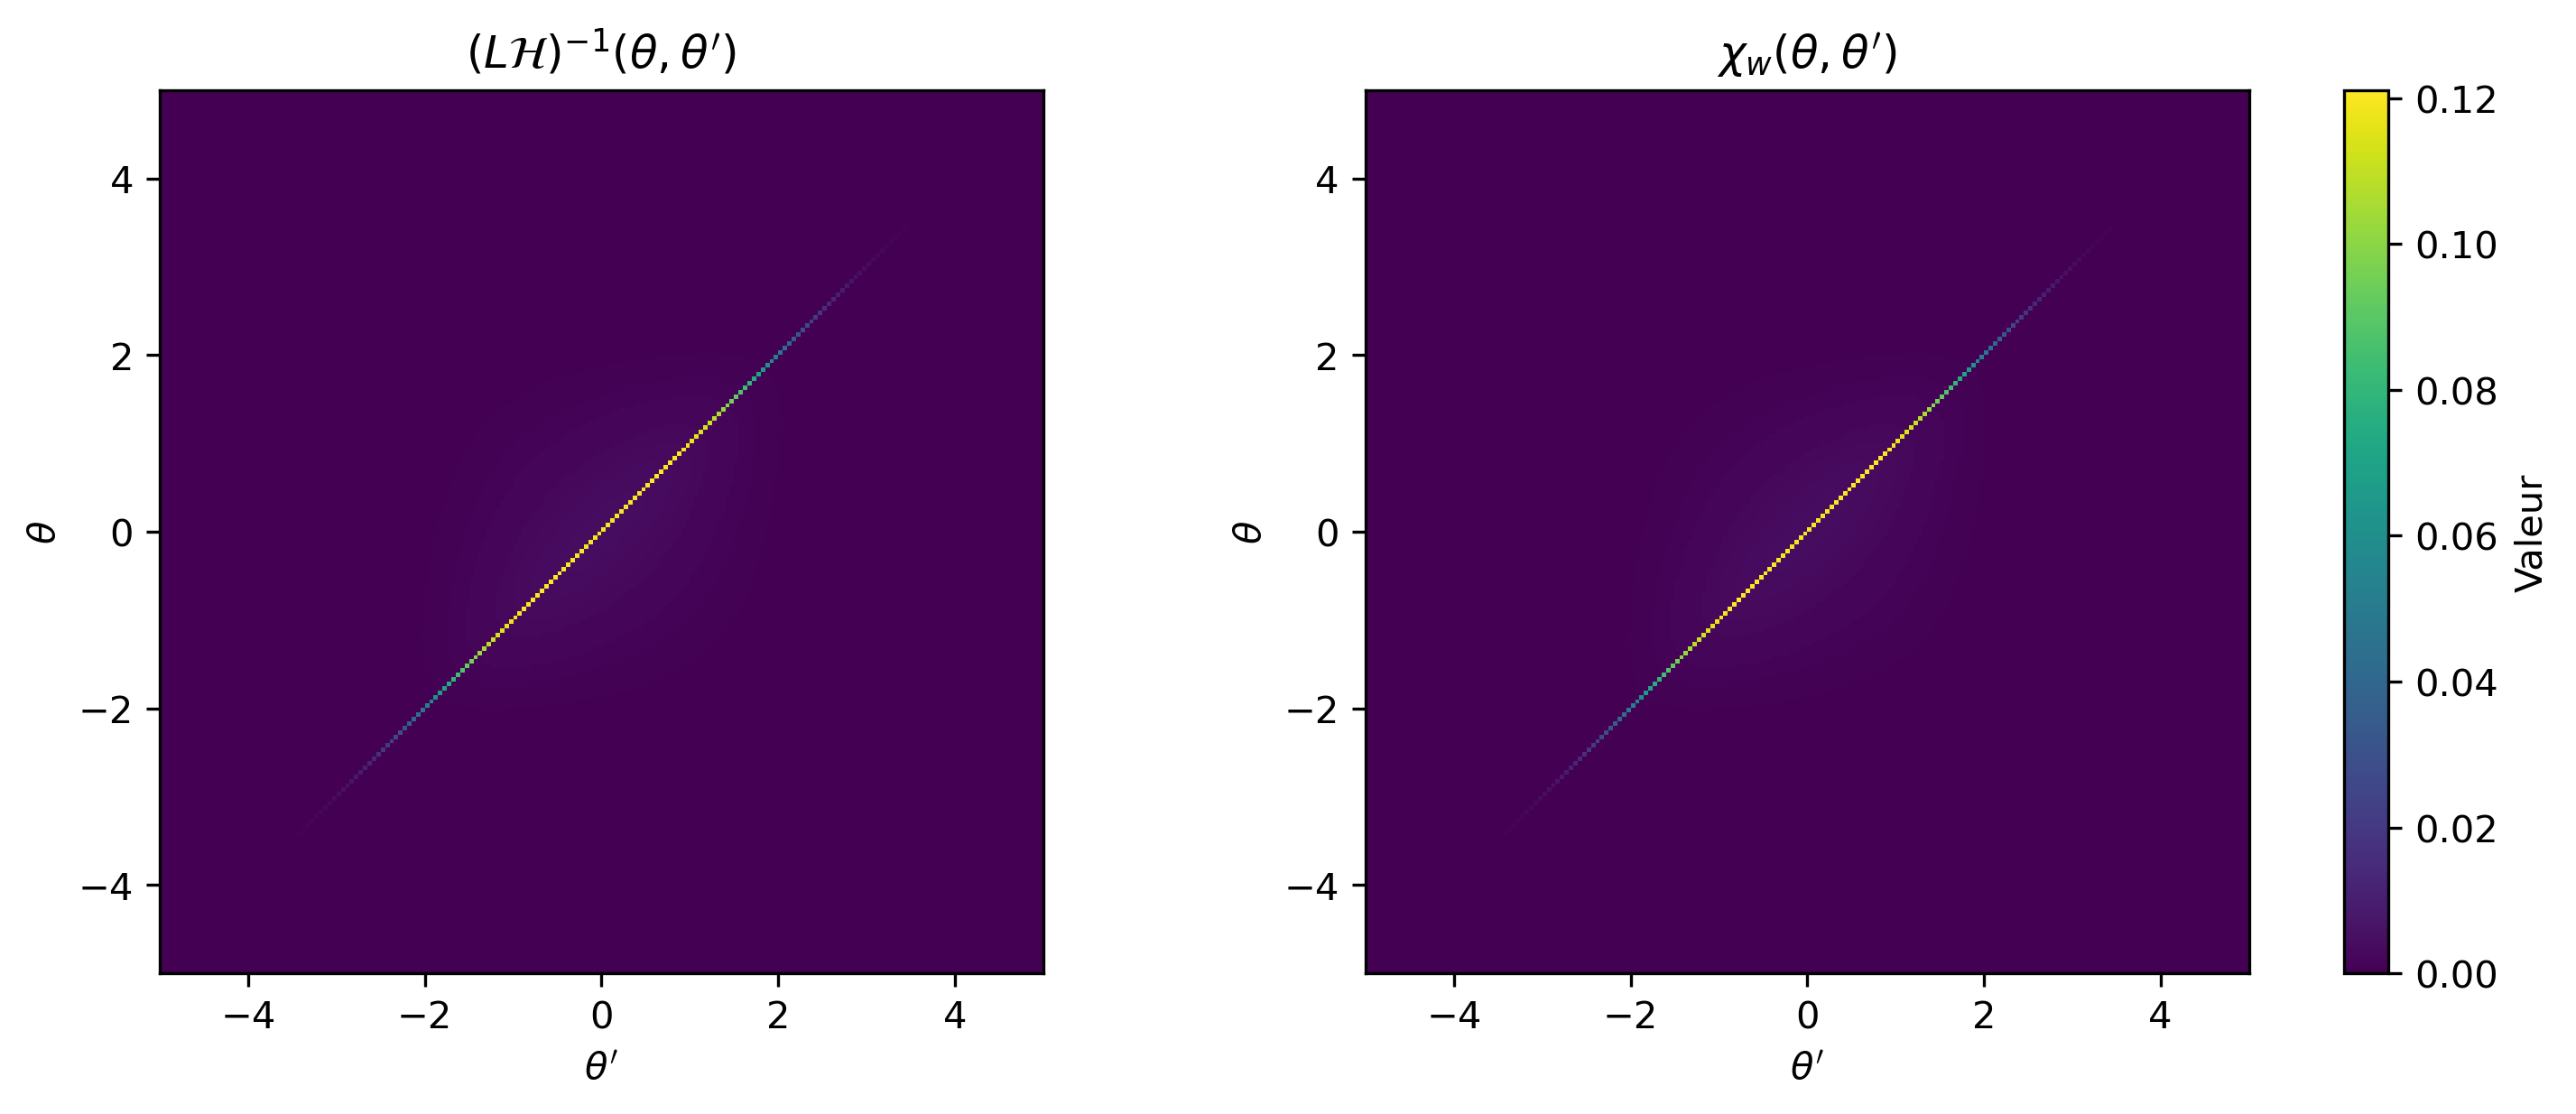
\includegraphics[width=1\textwidth]{figures/04_GGE_Fluctuation/heatmaps_2.png}
    \caption{Vérification numérique dans le régime thermodynamique. Gauche : $(L\mathcal{H})^{-1}$ par inversion de la courbure. Droite : \(\chi_w\) par dérivée fonctionnelle.}
    \label{fig:chi_thermodynamique}
\end{figure}

\paragraph{Conclusion.}

Nous avons vérifié la formule \eqref{chap:fluctu:eq:fluctuations.10} de deux manières. D’une part, en évaluant directement à un {\em poids spectral} $w$ fixé $(L\mathcal{H})^{-1}$; d’autre part, en calculant la différentielle de la distribution de rapidité par rapport au poids spectral \(\chi_w\), c’est-à-dire  en appliquant le principe de fluctuation–réponse. Pour le {\em poids spectral} et les paramètres considérés, les deux approches donnent des résultats numériques concordants, ce qui constitue une validation de la formule \eqref{chap:fluctu:eq:fluctuations.10}.

%Cette vérification confirme que, dans le régime thermodynamique, la structure variationnelle de l’entropie de \gls{YY} encode entièrement les fluctuations et les réponses spectrales du système. Il s’agit d’un test non trivial du principe de fluctuation–réponse appliqué aux systèmes intégrables.

\medskip

Dans un second temps, il est naturel de vouloir tester ce principe pour différentes formes du {\em poids spectral} $w$. Dans le cas général du \gls{GGE}, $w$ appartient à un espace de dimension infinie. Afin de réduire cette complexité, nous nous restreignons à une sous-famille à deux paramètres, en nous plaçant dans le cadre de l’équilibre thermique. Ce choix permet de comparer explicitement les fluctuations de grandeurs thermodynamiques macroscopiques, telles que le nombre total de particules et l’énergie cinétique.




%\section{Lien entre dérivée fonctionnelle et réponse linéaire aux facteurs de Lagrange}

\subsubsection{Vérification numérique thermique :  énergie et nombre de particules}

Nous testons à présent notre expression des fluctuations dans le cas particulier de l'équilibre thermique. Le sous-système est supposé en contact avec un bain à température \( T \) et potentiel chimique \( \mu \).
%Le poids spectral prend alors la forme canonique :
%\(
%w(\theta) = \beta \varepsilon(\theta) - \beta \mu,
%\)
%avec \( \beta = 1 / (k_B T) \) et \( \varepsilon(\theta) \) l’énergie (par exemple \( m\theta^2/2 \) pour des particules libres).

%\subparagraph{Paramètres fixés.}
%Dans le cas de l’équilibre thermique usuel (ensemble de Gibbs), seules deux charges sont conservées : le {\bf nombre total de particules} \( \operator{\mathcal{Q}}[f_0] \) et l’{\bf énergie totale} \( \operator{\mathcal{Q}}[f_2] \). Cela correspond au choix suivant :
%\begin{align*}
%	f_0(\theta) &= 1, \quad &&\text{(densité de particules)} \\
%	f_2(\theta) &= \frac{1}{2}m \theta^2, \quad &&\text{(densité d’énergie $\varepsilon$)}
%\end{align*}
%les coefficients de Lagrange associés sont :
%\begin{align*}
%	\beta_0 &= -\beta \mu, \quad &&\text{(potentiel chimique)} \\
%	\beta_2 &= \beta, \quad &&\text{(inverse de la température)},
%\end{align*}
%avec $\beta = 1 / ( k_B T )$ et  $k_B$ constante de Boltzmann.
%
%\medskip
%
%\paragraph{Calcul de la matrice hermitienne.}
%
%On reprend ici le formalisme de l’équation \eqref{chap4:eq.w_fi}, dans lequel le poids spectral s’écrit comme une combinaison linéaire :
%\begin{eqnarray}\label{chap4:eq.w.1}
%	w(\theta) & = & \beta_0 f_0(\theta) + \beta_2 f_2(\theta),
%\end{eqnarray}
%où \( f_0(\theta) = 1 \) et $f_2(\theta) = \frac{1}{2}m \theta^2,$ sont les densités locales associées aux charges conservées , fixeé et $\beta_0$ et $\beta_2$ en imposant une température \(T\) et un potentiel chimique \(\mu\).
%
%Dans les équations \eqref{chap2:eq:gamma.1} et \eqref{chap2:eq:t.1}, nous avons défini les grandeurs adimensionnées, le {\bf paramètre de Lieb} $\gamma$ et la {\bf température réduite} $t$, telles que :
%\begin{eqnarray*}
%	\gamma = \frac{m g}{\hbar^2 n}, \quad t = \frac{\hbar^2}{m \beta g^2}.
%\end{eqnarray*}
%
%\subparagraph{Paramètres fixes.}
%Nous travaillons avec $\hbar = m = k_B = 1$, et nous choisissons $L = 100$ et $g = 1$.
%
%\subparagraph{Paramètres variables.}
%La température $T$ est alors donnée par la température réduite $t$, et la densité linéaire $n$ est inversement proportionnelle au paramètre adimensionné $\gamma$.


%\paragraph{Calcul de la matrice hermitienne.}
%
%Les densités locales $f_i$ sont fixées. Pour spécifier le {\em poids spectral} $w$, on choisit les coefficients de Lagrange $\beta_0$ et $\beta_2$ en imposant une température \(T\) et un potentiel chimique \(\mu\).
%
%\medskip
%
%Dans les équations \eqref{chap2:eq:gamma.1} et \eqref{chap2:eq:t.1}, nous avons défini les grandeurs adimensionnées, le {\bf paramètre de Lieb} $\gamma$ et la {\bf température réduite} $t$, telles que :
%\begin{eqnarray*}
%	\gamma = \frac{m g}{\hbar^2 n}, \quad t = \frac{\hbar^2}{m \beta g^2}.
%\end{eqnarray*}



%La densité linéaire \( n \) ne paramétrise pas directement le poids spectral $w$ \eqref{chap4:eq.w.1}, mais est liée au potentiel chimique \(\mu\) via :
%\[
%	L n = \braket{\operator{\mathcal{Q}}[f_0]}_w.
%\]
%C’est ainsi que les simulations numériques seront effectuées en utilisant $\gamma$ et $t$.

%\subparagraph{Paramètres variables.}
%Avec ces conventions, la densité linéaire $n$ est reliée directement au paramètre $\gamma$, tandis que la température physique $T$ est déterminée par la température réduite $t$. Ainsi, dans l’équation~\eqref{chap4:eq.w.1}, les fonctions $f_i(\theta)$ sont fixées, et ce sont les coefficients $\beta_i$ qui s’ajustent en fonction des paramètres adimensionnés $\gamma$ et $t$, c’est-à-dire en fonction des conditions thermodynamiques imposées.



\paragraph{Calcul de la matrice hermitienne.}

Dans la section~\ref{chap4:sec:TBA}, nous avons présenté les différentes étapes de la résolution numérique de l’équation de \gls*{TBA}.
Nous reprenons ici le formalisme de l’équation~\eqref{chap4:eq.w_fi}, dans lequel le poids spectral s’écrit comme une combinaison linéaire :
\begin{equation}\label{chap4:eq.w.1}
	w(\theta) = \beta_0 f_0(\theta) + \beta_2 f_2(\theta),
\end{equation}
où $f_0(\theta) = 1$ et $f_2(\theta) = \tfrac{1}{2} m \theta^2$ correspondent aux densités locales associées aux charges conservées.
Les coefficients $\beta_0 = - \beta \mu $ et $\beta_2 = \beta (= (k_B T)^{-1})$ sont fixés de manière à imposer une température $T$ et un potentiel chimique $\mu$.

\medskip

Le \textbf{paramètre de Lieb} et la \textbf{température réduite}, définis respectivement en~\eqref{chap2:eq:gamma.1} et~\eqref{chap2:eq:t.1},
\begin{equation*}
	\gamma = \frac{m g}{\hbar^2 n},
	\qquad
	t = \frac{\hbar^2}{m \beta g^2},
\end{equation*}
permettent également de paramétrer le couple $(T,\mu)$ (voir section~\ref{chap4:sec:TBA}).

% \subparagraph{Paramètres fixes.}
% Dans toute la suite, nous travaillons avec les conventions $\hbar = m = k_B = 1$, ainsi que $L = 100$ et $g = 1$.

% \medskip

% \subparagraph{Choix des paramètres.}
% Nous considérons le point
% \begin{equation*}
% 	\gamma = 0.02,
% 	\qquad
% 	t = 70 ,
% \end{equation*}
% qui est représenté par un \textbf{point rouge} dans le diagramme de phase du modèle de \gls{LL}, présenté en figure~\ref{chap:4:fig:diagr}.

\begin{tcolorbox}[colback=blue!5!white,colframe=blue!75!black,title=Remarque]
On rappelle que le paramètre de Lieb \(\gamma\) caractérise la force d'interaction relative entre les particules, tandis que la température réduite \(t\) quantifie l'importance des effets thermiques par rapport aux interactions. En variant ces deux paramètres, on explore différents régimes physiques du système.
\end{tcolorbox}

\begin{tcolorbox}[colback=blue!5!white,colframe=blue!75!black,title=Remarque]
Dans cette continuité, nous allons définir des unités naturelles adaptées au système étudié. Ces unités facilitent l'interprétation physique des résultats numériques en les reliant directement aux grandeurs expérimentales.

\subparagraph{Conversion vers les unités réelles.}
Mais avant pour faciliter la comparaison avec les expériences, nous allons définir des unités caractéristiques:

\begin{eqnarray}
\ell_0 &= &  \frac{\hbar^2}{m g}, \quad \text{(longueur)}\\
\tau_0 &= &  \frac{m \ell_0^2}{\hbar},  \quad \text{(temps)}\\
E_0 &= & \frac{\hbar^2}{m L_0^2}, \quad \text{(énergie)}\\
T_0 &=&\frac{E_0}{k_B}, \quad \text{(température)}.
\end{eqnarray}

Mes résultats numériques sont exprimés en unités naturelles adimensionnées. Pour revenir aux valeurs réelles, il suffit de les multiplier par les unités caractéristiques définies ci-dessus.

% Ainsi, les paramètres naturels peuvent être convertis en unités réelles par
% \[
% x_\text{réel} = L_0 \, x_\text{nat}, 
% \qquad
% t_\text{réel} = T_0 \, t_\text{nat}, 
% \qquad
% T_\text{réel} = T_\text{nat} \, T_\text{nat},
% \]
% permettant de comparer directement nos résultats numériques avec les expériences.
\end{tcolorbox}	


\subparagraph{Paramètres fixes.}
Dans toute la suite, nous travaillons avec les conventions naturelles
\(\hbar = m = k_B = 1\), ainsi qu'avec
\begin{equation*}
L = 10, \qquad g = 1.
\end{equation*}

\medskip



\subparagraph{Choix des paramètres.}
Nous considérons le point
\begin{equation*}
    \gamma = 0.02,
    \qquad
    t = 70,
\end{equation*}
qui est représenté par un \textbf{point rouge} dans le diagramme de phase du modèle de \gls{LL}, présenté en figure~\ref{chap:4:fig:diagr}.


\begin{tcolorbox}[colback=blue!5!white,colframe=blue!75!black,title=Remarque]
Les paramètres choisis ne sont pas arbitraires : ils sont proches des régimes expérimentaux que nous considérons. 
La taille du sous-système \(L\) est en unité réelle de $22\,\mu m$, la densité linéaire \(n\) est de l'ordre de $23\,\mu m^{-1}$ et la température \(T\) est d'environ $81\,nK$.
\end{tcolorbox}

% \medskip

% \subparagraph{Conversion vers les unités réelles.}
% Pour relier ces valeurs aux grandeurs physiques réelles, on définit les unités naturelles :
% \[
% \begin{aligned}
% L_0 &= \frac{\hbar^2}{m g_\text{réel}}, &\text{(longueur)}\\
% T_0 &= \frac{m L_0^2}{\hbar}, &\text{(temps)}\\
% E_0 &= \frac{\hbar^2}{m L_0^2}, &\text{(énergie)}\\
% T_\text{nat} &= \frac{E_0}{k_B}, &\text{(température)}
% \end{aligned}
% \]

% Ainsi, les paramètres naturels peuvent être convertis en unités réelles par
% \[
% x_\text{réel} = L_0 \, x_\text{nat}, 
% \qquad
% t_\text{réel} = T_0 \, t_\text{nat}, 
% \qquad
% T_\text{réel} = T_\text{nat} \, T_\text{nat},
% \]
% permettant de comparer directement nos résultats numériques avec les expériences.





\medskip

À partir de ce paramètre, et suivant la même procédure numérique que dans la sous-section précédente, on obtient la distribution de rapidité à l'équilibre
\(\braket{\operator{\rho}(\theta)}_w \equiv \rho_{\mathrm{eq}}(\theta)\), ainsi que les composantes de l’inverse de l’opérateur hessien \((L\mathcal{H})^{-1}\) : la contribution diagonale sans interaction \((L\mathcal{D})^{-1}\) (Fig.~\ref{chap:4:fig:fluctu_diag}) et la contribution non locale issue des interactions \(\mathcal{B}/L\) (Fig.~\ref{chap:4:fig:fluctu_B}).

\medskip

Plus précisément, dans la figure~\ref{chap:4:fig:fluctu_diag}, on représente
\begin{eqnarray*}
	\frac{\mathcal{D}^{-1}(\theta, \theta')}{\delta(\theta - \theta')} \quad  \left( =  \rho_{s, \mathrm{eq}}(\theta) \, \nu_{\mathrm{eq}}(\theta) \, (1 - \nu_{\mathrm{eq}}(\theta)) \right),
\end{eqnarray*}
la fonction delta dans \eqref{chap:fluctu:eq:irreg.inv} étant approximée numériquement par un pas de discrétisation, la matrice \(\mathcal{D}^{-1}\) est proportionnelle à ce pas.

\medskip

Enfin, en faisant varier $t$ (\ie la température \(T\)), on répète l'ensemble des calculs précédents.
Les régimes ainsi obtenus sont indiqués par des {\bf points bleus} dans le diagramme de phase (figure~\ref{chap:4:fig:diagr}).



\paragraph{Corrélation des observables thermodynamiques.}

\medskip
Conformément à l’équation~\eqref{chap4:eq.cumulant.distr.q.10}, nous calculons les fluctuations du nombre total de particules ainsi que celles de l’énergie totale, respectivement données par :
\begin{eqnarray}
	C_w[f_0,f_0]  & = & L^2 \iint d\theta\, d\theta'\; f_0(\theta)\, (L\mathcal{H})^{-1}(\theta , \theta')\, f_0(\theta') ,\\
	C_w[f_2,f_2]  & = & L^2 \iint d\theta\, d\theta'\; f_2(\theta)\,(L\mathcal{H})^{-1}(\theta , \theta')\, f_2(\theta').
\end{eqnarray}

Pour chaque régime simulé (correspondant aux {\bf points bleus} et {\bf rouge} sur la figure~\eqref{chap:4:fig:diagr}), nous évaluons numériquement les quantités \( C_w[f_0,f_0] \) et \( C_w[f_2,f_2] \), qui représentent les fluctuations extensives des observables associées aux charges \( \operator{Q}_0 \) (nombre de particules) et \( \operator{Q}_2 \) (énergie cinétique).

\medskip

Ces résultats sont représentés par des {\bf points rouges} dans la figure~\ref{chap:4:fig.fluctu.A_com}, illustrant l’évolution des fluctuations en fonction du régime thermodynamique du sous-système.


\paragraph{Susceptibilité des observables thermodynamiques.}

\medskip
En parallèle, pour chaque régime simulé (correspondant aux {\bf points bleus} et {\bf rouge} de la figure~\eqref{chap:4:fig:diagr}), et conformément à l’équation~\eqref{chap4:eq.moment.distr.q.10}, nous calculons les moyennes des charges associées au nombre total de particules et à l’énergie cinétique totale, données respectivement par :
\begin{eqnarray}
	\braket{\operator{\mathcal{Q}}[f_0]}_w & = & L \int d\theta\; f_0(\theta)\, \braket{\operator{\rho}(\theta)}_w,\\
	\braket{\operator{\mathcal{Q}}[f_2]}_w & = & L \int d\theta\; f_2(\theta)\, \braket{\operator{\rho}(\theta)}_w.
\end{eqnarray}

\medskip

Nous souhaitons ensuite évaluer les susceptibilités thermodynamiques définies par :
\begin{eqnarray}
	\chi_w[f_i, f_i] & = & - \left. \frac{\partial \braket{\operator{\mathcal{Q}}[f_i]}_w}{\partial \beta_i} \right)_{\beta_{j \neq i} \text{ fixés}}.
\end{eqnarray}

Pour cela, nous procédons à une variation infinitésimale du poids spectral $w$ :

\begin{itemize}[label =$\bullet$]
	\item Une variation infinitésimale $\epsilon_\mu$ du potentiel chimique $\mu$ correspond à une perturbation du poids spectral de la forme :
	\[
	w \rightarrow w - \beta \epsilon_\mu f_0.
	\]
	On résout alors numériquement les équations \gls{TBA} pour ce nouveau poids, afin de calculer :
	\[
	\braket{\operator{\mathcal{Q}}[f_0]}_{w - \beta \epsilon_\mu f_0}.
	\]

	\item On effectue ensuite une variation infinitésimale $\epsilon_\beta$ de l’inverse de la température, de sorte que la combinaison \( (\beta + \epsilon_\beta)(\mu + \epsilon_\mu) = \beta \mu \) reste constante, maintenant ainsi $\beta_0$ fixe. Cela conduit à une variation du poids spectral de la forme :
	\[
	w \rightarrow w + (\beta + \epsilon_\beta)(- \epsilon_\mu f_0 + f_2).
	\]
	On résout à nouveau les équations TBA pour obtenir :
	\[
	\braket{\operator{\mathcal{Q}}[f_2]}_{w + (\beta + \epsilon_\beta)(- \epsilon_\mu f_0 + f_2)}.
	\]
\end{itemize}

\medskip

Ces simulations permettent d’estimer numériquement les susceptibilités :
\begin{eqnarray}
	\chi_w[f_0, f_0]	 & \approx & \frac{\braket{\operator{\mathcal{Q}}[f_0]}_{w - \beta \epsilon_\mu f_0} - \braket{\operator{\mathcal{Q}}[f_0]}_w}{\beta \epsilon_\mu},	\\
	\chi_w[f_2, f_2]	 & \approx & - \frac{\braket{\operator{\mathcal{Q}}[f_2]}_{w + (\beta + \epsilon_\beta)(- \epsilon_\mu f_0 + f_2)} - \braket{\operator{\mathcal{Q}}[f_2]}_w}{\epsilon_\beta}.
\end{eqnarray}

\medskip

Ces approximations numériques sont représentées par des {\bf points bleus} dans la figure~\eqref{chap:4:fig.fluctu.A_com}, et permettent de comparer les résultats issus de la dérivée fonctionnelle avec ceux provenant de la réponse directe à une perturbation du poids spectral.



%Conformément à l'équation \eqref{chap4:eq.moment.distr.q.10} la densité linéaire $n$

%Pour explorer différents  zone du diagramme de phase du modèle de Lieb-Liniger



%\paragraph{Cas du nombre de particules.}
%On choisit la fonction test \( f_{\operator{Q}}(\theta) = 1 \), ce qui définit la charge associée :
%\[
%\operator{Q} = \operator{\mathcal{Q}}[1] = L \int d\theta\, \operator{\rho}(\theta).
%\]
%Son facteur de Lagrange / potentiel conjugué dans \( w(\theta) \) est simplement :
%\[
%w(\theta) \supset -\beta \mu \cdot 1.
%\]
%La susceptibilité  et les corrélations associée sont égaux:
%\[
%\chi_w[{\operator{Q},\operator{Q}}] \doteq \left . \frac{\partial \langle \operator{Q} \rangle_w}{\partial (\beta \mu)} \right)_\beta  = L^2 \iint d\theta\, d\theta'\, C_w(\theta, \theta') \doteq C_w(f_{\operator{Q}}, f_{\operator{Q}}).
%\]
%
%\paragraph{Cas de l’énergie.}
%On prend maintenant \( f_{\operator{H}}(\theta) = \varepsilon(\theta) \), l’énergie spectrale (ici par ex. \( \theta^2/2 \) pour des particules libres), ce qui donne :
%\[
%\operator{H} = \operator{\mathcal{Q}}[\varepsilon] = L \int d\theta\, \varepsilon(\theta)\, \operator{\rho}(\theta),
%\]
%et facteur de Lagrange / potentiel conjugué  est simplement \( \beta \varepsilon(\theta) \), avec :
%\[
%w(\theta) \supset \beta \varepsilon(\theta).
%\]
%On en déduit la susceptibilité thermique :
%\[
%\chi_{\operator{H},\operator{H}} \doteq -\left.\frac{\partial \langle \operator{H} \rangle_w}{\partial \beta} \right)_{\beta \mu}  = L^2 \iint d\theta\, d\theta'\, \varepsilon(\theta)\, C_w(\theta, \theta')\, \varepsilon(\theta') \doteq C_w(f_{\operator{H}}, f_{\operator{H}}).
%\]

%\paragraph{Évaluation numérique.}

%On fais les calcule des correlation pour $\gamma = g/n $ fixé à ?? et $t = 1/(\beta g^2)$ entre ?? et ??.Les points correspondants sont représentés en bleu sur un diagramme de phase du modèle de Lieb-Liniger (voir Fig.~\ref{fig:diag}).

%Ce même diagramme contient également un point rouge correspondant à \( t = ?? \). Les fluctuations associées à ce point sont représentées en niveaux de couleur sur un graphique 2D (voir Fig.~\ref{fig.fluctu.A})

%Les corrélations de \( \rho(\theta) \) sont calculées numériquement pour un couplage \(\gamma = g/n\) fixé, et une température réduite \( t = 1 / (\beta g^2) \) variant dans un intervalle donné. Les points correspondants sont indiqués en \textbf{bleu} dans le diagramme de phase du modèle de Lieb-Liniger (Fig.~\ref{fig:diag}).
%
%Dans ce même diagramme, un \textbf{point rouge} correspond à des conditions fixes (\(T = 60~\mathrm{nK}\), \( \mu = 27~\mathrm{nK} \)), pour lesquelles la carte des fluctuations \( \delta \rho \) est représentée en niveaux de couleur (Fig.~\ref{fig.fluctu.A}).


%\begin{figure}[H]
%	\centering
%	\begin{subfigure}[b]{0.25\textwidth}
%		
\includegraphics[width=\textwidth]{Figures/04_GGE_Fluctuation/diagram.png}
%		\caption{Diagramme de phase du modèle de Lieb-Liniger.}
%		\label{chap:4:fig:diagr}
%	\end{subfigure}
%	\hfill
%	\begin{subfigure}[b]{0.3\textwidth}
%		
\includegraphics[width=\textwidth]{Figures/04_GGE_Fluctuation/diag_fluctu_1.png}
%		\caption{ \( \mathcal{D}^{-1}(\theta, \theta)/\delta(\theta, \theta) \).}
%		\label{chap:4:fig.fluctu.A}
%	\end{subfigure}
%	\hfill
%	\begin{subfigure}[b]{0.4\textwidth}
%		
\includegraphics[width=\textwidth]{Figures/04_GGE_Fluctuation/fluctu_1.png}
%		\caption{ \( \mathcal{B}(\theta, \theta') \).}
%		\label{chap:4:fig.fluctu.A}
%	\end{subfigure}
%	\caption{(a) Diagramme de phase du modèle de Lieb-Liniger à l’équilibre thermique. Différents régimes asymptotiques sont séparés par des transitions progressives. Les points bleus représentent les fluctuations calculées numériquement pour différentes températures. Les coordonnées sont données par \( \gamma = \frac{m g}{\hbar^2 n} \) et \( t = \frac{k_B T}{m g^2/\hbar^2} \). On Représenter les régimes choisir pour les simulation en point blue ( à \( \gamma = 10^{-1.7} \) constant et en rouge pour \( t = 89.125 \) un point représenté en (b) et (c). (b) Representation de diagolale $\mathcal{D}^{-1}(\theta, \theta)/\delta(\theta, \theta)$ et (c) Représentation en niveaux de couleur de la partie régulière $\mathcal{B}$ des fluctuations \( \delta \rho \) pour \( t = 89.125 \) et \( \gamma = 10^{-1.7} \) (point rouge dans (a)).}
%	\label{chap:4:fig:diag_fig}
%\end{figure}
%
%\begin{figure}[H]
%    \centering
%    \begin{subfigure}[b]{0.25\textwidth}
%        
\includegraphics[width=\textwidth]{Figures/04_GGE_Fluctuation/diagram.png}
%        \caption{Diagramme de phase du modèle de Lieb-Liniger à l’équilibre thermique.}
%        \label{chap:4:fig:diagr}
%    \end{subfigure}
%    \hfill
%    \begin{subfigure}[b]{0.3\textwidth}
%        
\includegraphics[width=\textwidth]{Figures/04_GGE_Fluctuation/diag_fluctu_1.png}
%        \caption{Diagonale \( \mathcal{D}^{-1}(\theta, \theta)/\delta(\theta, \theta) \) des fluctuations.}
%        \label{chap:4:fig:fluctu_diag}
%    \end{subfigure}
%    \hfill
%    \begin{subfigure}[b]{0.4\textwidth}
%        
\includegraphics[width=\textwidth]{Figures/04_GGE_Fluctuation/fluctu_1.png}
%        \caption{Représentation en niveaux de couleur de la partie régulière \( \mathcal{B}(\theta, \theta') \) des fluctuations \( \delta \rho \) pour \( t = 89.125 \) et \( \gamma = 10^{-1.7} \).}
%        \label{chap:4:fig:fluctu_B}
%    \end{subfigure}
%    \caption{(a) Diagramme de phase du modèle de Lieb-Liniger, avec les différents régimes asymptotiques séparés par des transitions progressives. Les points bleus indiquent les valeurs des fluctuations calculées numériquement pour différentes températures. Les coordonnées sont données par \( \gamma = \frac{m g}{\hbar^2 n} \) et \( t = \frac{k_B T}{m g^2/\hbar^2} \). Le point rouge correspond aux paramètres utilisés pour les sous-figures (b) et (c). (b) Diagonale de \( \mathcal{D}^{-1}(\theta, \theta)/\delta(\theta, \theta) \). (c) Partie régulière \( \mathcal{B}(\theta, \theta') \) des fluctuations \( \delta \rho \).}
%    \label{chap:4:fig:diag_fig}
%\end{figure}

\begin{figure}[H]
    \centering
    \begin{subfigure}[b]{0.25\textwidth}
        
\includegraphics[width=\textwidth]{Figures/04_GGE_Fluctuation/diagram.png}
        \caption{Diagramme de phase du modèle de Lieb-Liniger.}
        \label{chap:4:fig:diagr}
    \end{subfigure}
    \hfill
    \begin{subfigure}[b]{0.3\textwidth}
        
\includegraphics[width=\textwidth]{Figures/04_GGE_Fluctuation/diag_fluctu_1.png}
        \caption{\( \mathcal{D}^{-1}(\theta, \theta)/\delta(\theta, \theta) \).}
        \label{chap:4:fig:fluctu_diag}
    \end{subfigure}
    \hfill
    \begin{subfigure}[b]{0.4\textwidth}
        
\includegraphics[width=\textwidth]{Figures/04_GGE_Fluctuation/fluctu_1.png}
        \caption{\( \mathcal{B}(\theta, \theta') \).}
        \label{chap:4:fig:fluctu_B}
    \end{subfigure}
    \caption{
    (a) Diagramme de phase du modèle de \acrlong{LL} à l’équilibre thermique. Différents régimes asymptotiques sont séparés par des transitions progressives. Les points bleus représentent les fluctuations calculées numériquement pour différentes températures. Les coordonnées sont données par \( \gamma = \frac{m g}{\hbar^2 n} \) et \( t = \frac{k_B T}{m g^2/\hbar^2} \). Les régimes choisis pour les simulations sont indiqués par les points bleus (\( \gamma = 0.02 \) constant) et le point rouge correspond à \( t = 70 \), utilisé dans les sous-figures (b) et (c).
    (b) Représentation de la diagonale \( \mathcal{D}^{-1}(\theta, \theta)/\delta(\theta, \theta) \).
    (c) Représentation en niveaux de couleur de la partie régulière \( \mathcal{B} \) des fluctuations de\( \delta \rho \) pour \( t = 70 \) et \( \gamma = 0.02 \) (point rouge dans (a)).
    }
    \label{chap:4:fig:diag_fig}
\end{figure}



\paragraph{Comparaison avec les dérivées thermodynamiques.}

Les résultats obtenus à partir de l’analyse quadratique de l’action (fluctuations de \( \rho \)) sont comparés aux fluctuations extraites directement par différentiation des observables thermodynamiques \( \langle \operator{Q} \rangle_w \) et \( \langle \operator{H} \rangle_w \). Ces comparaisons sont présentées dans la Fig.~\ref{chap:4:fig.fluctu.A_com} et révèlent une excellente concordance. On le quantifie avec :
\begin{eqnarray*}
	\left \vert \frac{C_w[f_0,f_0] -  \chi_w[f_0,f_0]}{C_w[f_0,f_0]} \right \vert < 0.004\% , \quad \left \vert \frac{C_w[f_2,f_2] -  \chi_w[f_2,f_2]}{C_w[f_2,f_2]} \right \vert < 0.14 \%.
\end{eqnarray*}

%Les résultats obtenus à l’aide de cette méthode thermodynamique sont comparés à ceux issus du calcul direct des fluctuations de \( \rho \). Ces comparaisons sont représentées sur la Fig.~\ref{fig.fluctu.A_com}, et montrent une excellente concordance entre les deux approches.

\begin{figure}[H]
	\centering
	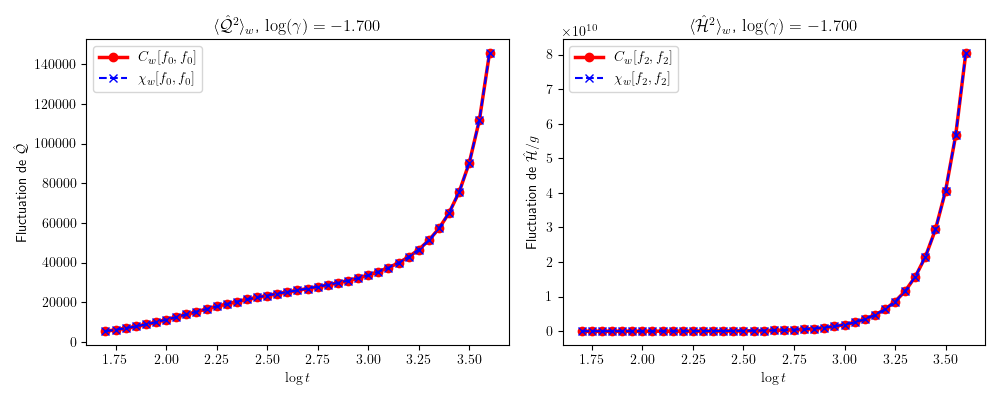
\includegraphics[width=1\textwidth]{figures/04_GGE_Fluctuation/fluctuations_plot_log_gamma=-1.700.png}
	%
\includegraphics[width=1\textwidth]{Figures/04_GGE_Fluctuation/fluctuations_relativ_plot_log_gamma=-1.342.png}
	\caption{Comparaison numérique entre  $C_w[f_0,f_0]$ et $\chi_w[f_0,f_0]$ et entre $C_w[f_2,f_2]$ et $\chi_w[f_2,f_2]$.}
	\label{chap:4:fig.fluctu.A_com}
\end{figure}



\section*{Conclusion}

Dans ce chapitre, nous avons étudié les fluctuations de la distribution de rapidité dans les états \gls{GGE}, en mettant en lumière le lien fondamental entre corrélations et réponse linéaire.

\medskip

Nous avons d’abord introduit le formalisme général des \gls{GGE}, dans lequel les observables macroscopiques sont dérivées fonctionnellement du potentiel conjugué $w(\theta)$. Dans ce cadre, nous avons montré que la matrice de susceptibilité spectrale $\chi_w(\theta , \theta')$ décrit à la fois la réponse linéaire de la densité spectrale moyenne à une perturbation infinitésimale du potentiel et les corrélations entre fluctuations de la densité, conformément au principe de \emph{fluctuation-réponse}. En utilisant ce lien, nous avons vu que nous pouvons  \emph{échantillonner \gls{GGE}}.

\medskip

Nous avons ensuite approfondi l’étude de la limite thermodynamique, où les fluctuations autour de l’état d’équilibre deviennent gaussiennes. Dans cette approximation, les susceptibilités s’expriment comme l’inverse de la courbure fonctionnelle de l’entropie de Yang-Yang, formalisée par l’opérateur hessien $\mathcal{H}^{(\mathcal{S}_{YY})}$. Nous avons donné une formulation explicite de cet opérateur, ainsi que de sa matrice inverse.

\medskip

Enfin, nous avons relié ces objets locaux à des susceptibilités globales via une projection sur les fonctions test $f_i(\theta)$, en considérant le poids spectral $w(\theta)$ comme une combinaison linéaire des charges $\operator{Q}_i$ . Ce formalisme nous a permis d’interpréter la dérivée de l’observable $\langle \operator{Q}_i \rangle_w$ par rapport au multiplicateur de Lagrange $\beta_i$ comme une dérivée fonctionnelle projetée de la matrice $\chi_w(\theta , \theta')$, et d’en valider la structure par une comparaison numérique explicite pour l’énergie et le nombre de particules.

\medskip

Nous avons vérifié numériquement la validité de notre formule des fluctuations (eq~\eqref{chap:fluctu:eq:fluctuations.10}), ce qui confirme son exactitude et sa pertinence dans le cadre du formalisme développé.


%\paragraph{🔸 Remarque sur les corrélations globales.}
%Dans les deux cas, les fluctuations totales \( \langle \delta N^2 \rangle \), \( \langle \delta E^2 \rangle \), ou croisées \( \langle \delta E\, \delta N \rangle \), sont données par les projections :
%\[
%\langle \delta Q_i\, \delta Q_j \rangle = \chi_{ij} = L^2 \iint d\theta\, d\theta'\, f_i(\theta)\, \chi(\theta, \theta')\, f_j(\theta').
%\]
%Cela généralise l’idée de la **formule de fluctuation-réponse** : la réponse à un potentiel conjugué est gouvernée par les corrélations spontanées du système au point d’équilibre.
%
%\paragraph{✅ Conclusion.}
%Pour toute charge \( \mathcal{Q}[f] = L \int f(\theta)\, \operator{\rho}(\theta)\, d\theta \), on a :
%\[
%\boxed{
%\chi_{f,f} = -\frac{\partial \langle \mathcal{Q}[f] \rangle}{\partial \lambda} = L^2 \iint d\theta\, d\theta'\, f(\theta)\, \chi(\theta, \theta')\, f(\theta'),
%}
%\]
%où \( \lambda \) est le coefficient dans \( w(\theta) = \lambda f(\theta) \).
%




%------------------------
%
%
%\section{Fonction correlation du nombre d'atomes et de l'énergie}
%
%
%Il est maintenant pertinent de tester notre expression des fluctuations. On fait l'hypothèset que le système est en équilibre thermique caractérisé par la températeur $T$ et le potentiel chimoque $\mu$.
%
%La valeur propre $\mathcal{N}[\rho]$ (resp $\mathcal{E}[\rho]$) de opérateur nombre d'atomes $\operator{\mathcal{N}}$ (resp énergie. $\operator{\mathcal{E}}$) et assiciés aux configuration liès à la distribution de rapidité $\rho$ s'écrit (avec comme combention la masse des atomes $k_B = \hbar = m =1$)
%
%\begin{eqnarray*}
%	\mathcal{N}[\rho] & = & L \int d \theta \rho(\theta),\\
%	\mathcal{E}[\rho] & = & 	\frac{L}2 \int d \theta  \theta^2 \rho(\theta).
%\end{eqnarray*}
%
%Les corrélation associèes s'est
%\begin{eqnarray*}
%	C_{\operator{\mathcal{N}},\operator{\mathcal{N}}} & = &  L^2 \int d\theta_a \int d\theta_b \, \langle \delta \rho(\theta_a) \delta \rho(\theta_b) \rangle, \\
%	C_{\operator{\mathcal{E}},\operator{\mathcal{E}}} & = &  	\left(\frac{L}2\right)^2 \int d\theta_a \int d\theta_b \,  \theta_a^2 \theta_b^2 \, \langle \delta \rho(\theta_a) \delta \rho(\theta_b) \rangle, \\
%\end{eqnarray*}
%
%
%
%%Les fluctuations des observables "nombre d’atomes" \( \operator{\mathcal{N}} \) et "énergie" \( \operator{\mathcal{E}} \) peuvent être exprimées à l’aide des fluctuations de \( \rho \) :
%
%%\begin{eqnarray*}
%%    \left \langle  \left( \operator{\mathcal{N}} - \langle \operator{\mathcal{N}} \rangle \right)^2 \right \rangle &=& L^2 \int d\theta_a \int d\theta_b \, \langle \delta \rho(\theta_a) \delta \rho(\theta_b) \rangle, \\
%%    \left \langle \left( \operator{\mathcal{E}} - \mu \operator{\mathcal{N}} - \langle \operator{\mathcal{E}} - \mu \operator{\mathcal{N}} \rangle \right)^2 \right \rangle &=& L^2 \int d\theta_a \int d\theta_b \, \left( -\mu + \frac{1}{2} m \theta_a^2 \right) \left( -\mu + \frac{1}{2} m \theta_b^2 \right) \langle \delta \rho(\theta_a) \delta \rho(\theta_b) \rangle,
%%\end{eqnarray*}
%
%%où \( \langle \operator{\mathcal{O}}_i \rangle \) désigne la moyenne de l’observable \( \operator{\mathcal{O}}_i \), \( m \) la masse des atomes et \( \mu \) le potentiel chimique.\\
%
%Dans la section \{??\}, nous avons vu que la variance d’une observable \( \operator{\mathcal{O}}_i \), autrement dit ses fluctuations, peut également s’exprimer comme une dérivée thermodynamique de sa moyenne :
%
%\begin{eqnarray*}
%    C_{\operator{\mathcal{O}}_i,\operator{\mathcal{O}}_i} = \Delta_{\operator{\mathcal{O}}_i}^2 = - \left. \frac{\partial \langle \operator{\mathcal{O}}_i \rangle}{\partial \beta_i} \right|_{\beta_{j \neq i}},
%\end{eqnarray*}
%
%où \( \beta_i \) est la variable conjuguée à \( \langle \operator{\mathcal{O}}_i \rangle \). En particulier, les fluctuations du nombre d’atomes et de l’énergie peuvent s’écrire :
%
%\begin{eqnarray*}
%    \Delta_{\operator{\mathcal{N}}}^2 &=& \frac{1}{\beta} \left. \frac{\partial \langle \operator{\mathcal{N}} \rangle}{\partial \mu} \right|_T, \\
%    \Delta_{\operator{\mathcal{E}}}^2 &=& \Delta_{\operator{\mathcal{E}} - \mu \operator{\mathcal{N}}}^2 + \mu \Delta_{\operator{\mathcal{N}}}^2 =   - \left. \frac{\partial \langle \operator{\mathcal{E}} - \mu \operator{\mathcal{N}} \rangle}{\partial \beta} \right|_\mu - \frac{\mu}{\beta} \left. \frac{\partial \langle \operator{\mathcal{N}} \rangle}{\partial \mu} \right|_T,
%\end{eqnarray*}
%
%avec \( \beta =T^{-1} \).
%
%Les quantités \( C_{\operator{\mathcal{N}},\operator{\mathcal{N}}} \) et \( \Delta_{\operator{\mathcal{N}}}^2 \) sont analytiquement équivalentes, de même que \( C_{\operator{\mathcal{E}},\operator{\mathcal{E}}} \) et \( \Delta_{\operator{\mathcal{E}}}^2 \).
%
%Nous souhaitons maintenant effectuer une comparaison numérique entre ces deux approches. Pour ce faire, nous avons d'abord résolu numériquement l’équation \{??\} avec \( f(\theta) = \beta \epsilon(\theta) - \beta\mu \), ce qui nous a permis d’obtenir \( \rho(\theta) \) et \( \rho_s(\theta) \) (Il y auras plus de détaille dans le chapitre ??) .
%
%%Nous avons ensuite calculé les fluctuations de \( \rho \) pour une densité spatiale fixée à \( n = 10~\mu \mathrm{m}^{-1} \), et pour différentes températures \( T \) allant de \( 5.7~\mathrm{K} \) à \( 53.5~\mathrm{nK} \). Le potentiel chimique \( \mu \) est ici une fonction de \( T \) et de \( n \). Les points correspondants sont représentés en bleu sur un diagramme de phase du modèle de Lieb-Liniger. En abscisse, nous avons le logarithme décimal du paramètre d’interaction de Lieb-Liniger \( \gamma = \frac{m g}{\hbar^2 n} \), et en ordonnée le logarithme décimal de \( t = \frac{\hbar^2}{\beta m g^2} \) (voir Fig.~\ref{fig:diag}).
%
%On fais les calcule des correlation pour $\gamma = g/n $ fixé à ?? et $t = 1/(\beta g^2)$ entre ?? et ??.Les points correspondants sont représentés en bleu sur un diagramme de phase du modèle de Lieb-Liniger (voir Fig.~\ref{fig:diag}).
%
%%Ce même diagramme contient également un point rouge correspondant à \( T = 60~\mathrm{nK} \) et \( \mu = 27~\mathrm{nK} \). Les fluctuations associées à ce point sont représentées en niveaux de couleur sur un graphique 2D (voir Fig.~\ref{fig.fluctu.A}).
%
%Ce même diagramme contient également un point rouge correspondant à \( t = ?? \). Les fluctuations associées à ce point sont représentées en niveaux de couleur sur un graphique 2D (voir Fig.~\ref{fig.fluctu.A})
%
%\begin{figure}[H]
%	\centering
%	\begin{subfigure}[b]{0.45\textwidth}
%		
\includegraphics[width=\textwidth]{Figures/diagram.png}
%		\caption{}
%		\label{fig:diag}
%	\end{subfigure}
%	\hfill
%	\begin{subfigure}[b]{0.45\textwidth}
%		
\includegraphics[width=\textwidth]{Figures/fluctu.png}
%		\caption{Fluctuations mesurées}
%		\label{fig.fluctu.A}
%	\end{subfigure}
%	\caption{(a) Diagramme de phase du modèle de Lieb-Liniger à l’équilibre thermique. Différents régimes asymptotiques sont séparés par des transitions progressives. Les points bleus représentent les fluctuations calculées numériquement pour différentes températures. Les coordonnées sont données par \( \gamma = \frac{m g}{\hbar^2 n} \) et \( t = \frac{k_B T}{m g^2/\hbar^2} \). (b) Représentation en niveaux de couleur des fluctuations \( \delta \rho \) pour \( T = 60~\mathrm{nK} \) et \( \mu = 27~\mathrm{nK} \) (point rouge dans (a)).}
%	\label{fig:diag_fig}
%\end{figure}
%
%%Nous calculons ensuite les moyennes des observables :
%
%%\begin{eqnarray*}
%%    \langle \operator{\mathcal{N}} \rangle &=& L \int \rho(\theta) \, d\theta, \\
%%    \langle \operator{\mathcal{E}} - \mu \operator{\mathcal{N}} \rangle &=& L \int \left( - \mu + \frac{1}{2} m \theta^2 \right) \rho(\theta) \, d\theta,
%%\end{eqnarray*}
%
%%pour chaque point du diagramme (Fig.~\ref{fig:diag}). En faisant varier leur variable conjuguée, nous accédons alors aux fluctuations $\Delta_{\operator{\mathcal{N}}}^2 $ et $\Delta_{\operator{\mathcal{E}} - \mu \operator{\mathcal{N}}}^2$.
%
%%\[
%%\Delta_{\operator{\mathcal{N}}}^2 = \frac{1}{\beta} \left. \frac{\partial \langle \operator{\mathcal{N}} \rangle}{\partial \mu} \right|_T, \quad
%%\Delta_{\operator{\mathcal{E}} - \mu \operator{\mathcal{N}}}^2 = - \left. \frac{\partial \langle \operator{\mathcal{E}} - \mu \operator{\mathcal{N}} \rangle}{\partial \beta} \right|_\mu.
%%\]
%
%Les résultats obtenus à l’aide de cette méthode thermodynamique sont comparés à ceux issus du calcul direct des fluctuations de \( \rho \). Ces comparaisons sont représentées sur la Fig.~\ref{fig.fluctu.A_com}, et montrent une excellente concordance entre les deux approches.
%
%\begin{figure}[H]
%	\centering
%	
\includegraphics[width=1\textwidth]{Figures/fluctuations_plot_log_gamma=-1.342.png}
%	%
\includegraphics[width=1\textwidth]{Figures/fluctuations_relativ_plot_log_gamma=-1.342.png}
%	\caption{Comparaison numérique entre les fluctuations calculées à partir de l’analyse quadratique de l’action (fluctuations de \( \rho \)) et celles obtenues par dérivées thermodynamiques des observables moyennes.}
%	\label{fig.fluctu.A_com}
%\end{figure}
%
%{\color{blue}
%%Dans ce chapitre, nous nous intéressons aux fluctuations de la distribution de rapidité \( \delta \rho \) autour d'une distribution de référence \( \rho^c \), qui maximise la contribution à la fonction de partition des états, exprimée comme une fonctionnelle de la distribution \( \rho \) :
%
%%La fonction de partition des états, s'exprime comme une fonctionnelle de la distribution \( \rho \) :
%
%%\begin{eqnarray*}\Xi & = & \sum_\rho \exp \left( -\mathcal{A}(\rho) \right).\end{eqnarray*}
%
%%Dans la section {\em \bf Entropie de Yang-Yang} (\ref{??}), l'action \( \mathcal{A}(\rho) \) s'écrit sous la forme :
%
%%\begin{eqnarray*}\mathcal{A}(\rho) & \doteq & - L\mathcal{S}_{YY}(\rho) + L\int f(\theta) \rho (\theta) \, d\theta,		\end{eqnarray*}
%
%%où \( \mathcal{S}_{YY} \) est la fonctionnelle d'entropie de Yang-Yang, définie dans (\ref{??}), et \( f \) est la fonction paramétrant les charges, introduite dans (\ref{??}).
%}
%{\color{blue}
%%Dans cette même section {\em \bf Entropie de Yang-Yang} (\ref{??}), nous avons établi un lien entre \( f \) et distribution de référence \( \rho^c \), qui maximise la contribution à la fonction de partition des états .\\
%
%}
%
%{\color{blue}
%
%%L'hypothèse qui après relaxation le système est décrit pas un GGE, est fondamantale dans notre compréhention, et a énormément d'implication. Et donc il est ittéressent de tester cette hyphotèse experimentalement.La distribution de rapidité moyenne $\rho^c$ ne permet pas de verifier que le GGE est bien l'enssemeble statistique adequa. En effet plein d'autre enssemble statistique donne la meme distribution de rapidité moyenne. Il faut donc aller au dela. Il faut regarder les fluctuation de distribution de rapidité \( \delta \rho \) autour \( \rho^c \)
%
%%L'hypothèse selon laquelle, après relaxation, le système est décrit par un ensemble généralisé de Gibbs (GGE) constitue un pilier fondamental de notre compréhension des dynamiques hors équilibre dans les systèmes intégrables. Cette hypothèse a des implications théoriques majeures, et il est donc essentiel de la confronter à l'expérience. Cependant, la seule connaissance de la distribution de rapidité moyenne $\rho^c$ ne permet pas de valider cette description. En effet, plusieurs ensembles statistiques peuvent conduire à une même distribution moyenne. Pour distinguer le GGE des autres candidats, il est nécessaire d’aller au-delà et d’analyser les fluctuations de la distribution de rapidité, notées \( \delta \rho \), autour de la valeur moyenne \( \rho^c \).
%
%
%%On veux tester si nos experience est décrit pas un GGE. Pour cela nous nous intéressons aux fluctuations de la distribution de rapidité \( \delta \rho \) autour \( \rho^c \).
%
%%Nous poursuivons à présent avec cette définition de l'action de classe $\mathcal{C}^2$ et admetant une distribution critique $\rho^c$ tel que sa différentielle en ce point critique soit nulle $d\mathcal{A}_{\rho^c} = 0 $ (\ref{??}) de sorte que d'aprés la formule de Taylor-Youg %afin de déterminer les fluctuations autour de \( \Pi^c \). Pour cela, nous réécrivons l'action sous la forme :
%
%%Nous poursuivons en développant l'action autour de la  distribution  $\rho^c$. La différentielle de l'action en ce point  est nulle ($d\mathcal{A}_{\rho^c} = 0 $ (\ref{??})).D'aprés la formule de Taylor-Youg , à l'ordre 2 en $\delta \rho$,  l'action s'écrit avec une forme quadratique : % tel que sa différentielle en ce point critique soit nulle ,  de sorte que d'aprés la formulle de Taylor-Youg %afin de déterminer les fluctuations autour de \( \Pi^c \). Pour cela, nous réécrivons l'action sous la forme :
%
%%\begin{eqnarray*}  \mathcal{A}(\rho^c + \delta \rho) & \underset{ \delta \rho \to 0 }{=} & \mathcal{A}(\rho^c)  + \frac{1}{2} \left. \frac{\delta^2 \mathcal{A}}{\delta \rho^2} \right|_{\rho^c} (\delta \rho) + \mathcal{O}((\delta \rho)^3),  \end{eqnarray*}
%
%%une expression quadratique pour l'action à l'ordre dominant en \( \delta \Pi \) avec $\left. \frac{\delta^2 \mathcal{A}}{\delta \rho^2} \right|_{\rho^c}$ la forme quadratique définie positive (Fig (\ref{fig.fluctu.A})).
%
%}
%
%{\color{blue}
%%On discrétise l'axe des rapidités en  petite cellule de rapidité $[\theta, \theta+\delta\theta]$, qui contient $L\rho(\theta) \delta \theta$ rapidités.
%
%
%
%
%%Avec ces petites tranches, la forme quadratique s’écrit :
%
%%\begin{eqnarray*}
%%    \left. \frac{\delta^2 \mathcal{A}}{{\delta \rho}^2} \right|_{\rho^c}(\delta \rho ) &=&  \sum_{a,b \mid \text{tranche}}
%%    \delta \rho(\theta_a)  \frac{\partial^2 \mathcal{A}}{\partial \delta \rho(\theta_a) \partial \delta \rho(\theta_b) } (\rho^c)  \delta \rho(\theta_b).
%%\end{eqnarray*}
%%Les fluctuations s’écrivent donc :
%
%%\begin{eqnarray*}
%%    \langle \delta \rho ( \theta) \delta \rho ( \theta') \rangle &=&
%%    \frac{ \int d\delta \rho \, \delta \rho(\theta) \delta \rho ( \theta')
%%    \exp \left( - \frac{1}{2} \sum_{a,b \mid \text{tranche}}
%%    \delta \rho(\theta_a) \frac{\partial^2 \mathcal{A}}{\partial \delta \rho(\theta_a) \partial \delta \rho(\theta_b) } (\rho^c)  \delta \rho(\theta_b) \right) }
%%    { \int d\delta \Pi
%%    \exp \left( - \frac{1}{2} \sum_{a,b \mid \text{tranche}}
%%    \delta \rho(\theta_a) \frac{\partial^2 \mathcal{A}}{\partial \delta \rho(\theta_a) \partial \delta \rho(\theta_b) } (\rho^c)  \delta \rho(\theta_b) \right) } \\
%%    &=& \left( \mathbf{A}^{-1} \right)_{\theta , \theta'}
%%\end{eqnarray*}
%
%
%%\begin{aff}
%
%%\begin{eqnarray*}\langle \delta \rho ( \theta) \delta \rho ( \theta') \rangle &=& 	\left( \mathbf{A}^{-1} \right)_{\theta , \theta'}\end{eqnarray*}
%
%
%%avec la  {\em matrice hessienne} $\mathbf{A}_{\theta , \theta'} \equiv \frac{\partial^2 \mathcal{A}}{\partial \delta \rho(\theta) \partial \delta \rho(\theta') }(\rho^c)$, au point critique/ qui maximise la probabilité  $\rho^c=\rho^c_s \nu^c $, s'écrit
%
%%avec la  matrice $\mathbf{A}_{\theta , \theta'} \equiv \frac{\partial^2 \mathcal{A}}{\partial \delta \rho(\theta) \partial \delta \rho(\theta') }(\rho^c)$, qui maximise la probabilité  $\rho^c=\rho^c_s \nu^c $, s'écrit
%
%%\begin{eqnarray*}
%%	\operator{A} & = & \operator{A}^{(0)} + \delta \theta \operator{V}
%%\end{eqnarray*}
%
%%avec
%
%%\begin{eqnarray*}
%%	A^{(0)}_{\theta , \theta'}  & = &  L\delta \theta \left ( \frac{ 1}{\rho^c_s ( 1  - \nu^c ) \nu^c } \right )(\theta)    \delta({\theta - \theta '})	,\\
%%	V_{\theta , \theta'}  &= & L \delta \theta \left \{ - \left [ \left ( \frac{1}{\rho^c_s( 1 - \nu^c) } \right ) ( \theta)  +  \left ( \frac{1}{\rho^c_s( 1 - \nu^c) } \right ) ( \theta' )\right ] \frac{ \Delta( \theta'- \theta )}{ 2 \pi } + \int d\theta''  \left ( \frac{\nu^c}{\rho^c_s( 1 - \nu^c) } \right )(\theta'') \frac{\Delta(\theta''- \theta)}{2 \pi}\frac{\Delta(\theta''- \theta')}{2 \pi}   \right \} 
%%\end{eqnarray*}
%
%%\end{aff}
%
%}
%
%
%{\color{blue}
%%Maintenant il est interressent de tester notre expression des fluctuation.\\
%%Dans la section {??} nous avons vus que la variance d'un observable $\operator{\mathcal{O}}_i$ s'écrit :
%
%%\begin{eqnarray*}
%%	\Delta_{\operator{\mathcal{O}}_i}^2 & = & -  \left . \frac{ \partial \langle \operator{\mathcal{O}}_i \rangle }{ \partial \beta_i } 	 \right )_{\beta_{j \neq i } }
%%\end{eqnarray*}
%
%%avec la moyenne $\langle \operator{\mathcal{O}}_i \rangle $ de  $\operator{\mathcal{O}}_i$ et $\beta_i$ la variable conjuguais de $\langle \operator{\mathcal{O}}_i \rangle $. Si on note les observables nombre d'atomes $\operator{\mathcal{N}}$ et énergie $\operator{\mathcal{E}}$, alors leur variance s'écrit
%
%
%%\begin{eqnarray*}
%%	\Delta_{\operator{\mathcal{N}}}^2  & = &  \frac{1}{\beta} \left . \frac{\partial \langle \operator{\mathcal{N}} \rangle}{\partial \mu} \right )_T \\
%%	\Delta_{\operator{\mathcal{E}}-\mu \operator{\mathcal{N}}}^2  & = &  - \left . \frac{\partial \langle \operator{\mathcal{E}}-\mu \operator{\mathcal{N}} \rangle}{\partial \beta} \right )_\mu
%%\end{eqnarray*}
%
%%avec $\beta = (k_B T)^{-1}$, la temperature $T$ et  le potentielle chimique $\mu$.\\
%
%%Et écrit à l'aide des fluctuation de $\rho$
%
%%\begin{eqnarray*}
%%	\tilde{\Delta}_{\operator{\mathcal{N}}}^2  &= & L^2 \int d\theta_a \int d \theta_b \, \langle \delta \rho(\theta_a) \delta \rho(\theta_b) \rangle \\
%%	\tilde{\Delta}_{\operator{\mathcal{E}}-\mu \operator{\mathcal{N}}}^2  & = & L^2 \int d\theta_a \int d \theta_b \, \left ( - \mu + \frac{1}2 m \theta_a^2  \right  )\left ( - \mu + \frac{1}2 m \theta_b^2  \right  )  \langle \delta \rho(\theta_a) \delta \rho(\theta_b) \rangle
%%\end{eqnarray*}
%
%%On veux comparer $\Delta_{\operator{\mathcal{N}}}^2$ à $\tilde{\Delta}_{\operator{\mathcal{N}}}^2$ et $\Delta_{\operator{\mathcal{E}}-\mu \operator{\mathcal{N}}}^2$ à $\tilde{\Delta}_{\operator{\mathcal{E}}-\mu \operator{\mathcal{N}}}^2 $. Pour ce faire, nous avons d'abord résolu numériquement l'équation {??} avec \( f(\theta) = \frac{\epsilon(\theta) - \mu}{T} \),  ce qui nous a permis d'obtenir \( \rho(\theta) \) et \( \rho_s(\theta) \). Si on fixe le couple $T$ et $\mu$. On peux donc deterniner les moyenne
%
%%\begin{eqnarray*}
%%	\langle \operator{\mathcal{N}} \rangle & = & L \int \, \rho(\theta) d \theta ,\\
%%	\langle \operator{\mathcal{E}} - \mu \operator{\mathcal{N}}\rangle & = & L \int \, \left (\frac{1}2 m \theta^2 - \mu  \right ) \rho(\theta) d\theta .
%%\end{eqnarray*}
%
%
%
%%Il est maintenant intéressant de tester notre expression des fluctuations.
%
%%Les fluctuations des observables nombre d'atomes $\operator{\mathcal{N}}$ et énergie $\operator{\mathcal{E}}$ peuvent s'écrire à l'aide de des fluctuation de $\rho$  :
%
%%\begin{eqnarray*}
%%    \left \langle  \left ( \operator{\mathcal{N}} - \langle \operator{\mathcal{N}}  \rangle  \right )^2 \right \rangle  &=& L^2 \int d\theta_a \int d\theta_b \, \langle \delta \rho(\theta_a) \delta \rho(\theta_b) \rangle, \\
%%    \left \langle  \left (  \operator{\mathcal{E}} - \mu \operator{\mathcal{N}}   -  \langle\operator{\mathcal{E}} - \mu \operator{\mathcal{N}}  \rangle  \right )^2  \right \rangle  &=& L^2 \int d\theta_a \int d\theta_b \, \left( - \mu + \frac{1}{2} m \theta_a^2 \right) \left( - \mu + \frac{1}{2} m \theta_b^2 \right) \langle \delta \rho(\theta_a) \delta \rho(\theta_b) \rangle,
%%\end{eqnarray*}
%
%%où \( \langle \operator{\mathcal{O}}_i \rangle \) est la moyenne de l'oservable  \( \operator{\mathcal{O}}_i \) ,  $m$ est la masse des atomes et $\mu$ est le potentielle chimique.\\
%
%%Dans la section {??}, nous avons vu que la variance d'un observable \( \operator{\mathcal{O}}_i \) autrement dit les fluctuation de \( \operator{\mathcal{O}}_i \) peuvent d'ecrire avec  derievés de leur moyenne  :
%
%%\begin{eqnarray*}
%%    \Delta_{\operator{\mathcal{O}}_i}^2 &=& - \left. \frac{\partial \langle \operator{\mathcal{O}}_i \rangle}{\partial \beta_i} \right|_{\beta_{j \neq i}}.
%%\end{eqnarray*}
%
%% où \( \beta_i \) est la variable conjuguée de \( \langle \operator{\mathcal{O}}_i \rangle \). Soit les fluctuation des observables nombre d'atome et énergie peuvent aussi s'écrire avec une dérivé de leur moyenne :
%
%%\begin{eqnarray*}
%%    \Delta_{\operator{\mathcal{N}}}^2 &=& \frac{1}{\beta} \left. \frac{\partial \langle \operator{\mathcal{N}} \rangle}{\partial \mu} \right|_T, \\
%%    \Delta_{\operator{\mathcal{E}} - \mu \operator{\mathcal{N}}}^2 &=& - \left. \frac{\partial \langle \operator{\mathcal{E}} - \mu \operator{\mathcal{N}} \rangle}{\partial \beta} \right|_\mu.
%%\end{eqnarray*}
%
%%avec \( \beta = (k_B T)^{-1} \), la température \( T \).
%
%%Les fluctuation \( \left \langle  \left ( \operator{\mathcal{N}} - \langle \operator{\mathcal{N}}  \rangle  \right )^2 \right \rangle  \) et  \( \Delta_{\operator{\mathcal{N}}}^2 \) sont analitiquement égaux et de meme pour  \( \left \langle  \left (  \operator{\mathcal{E}} - \mu \operator{\mathcal{N}}   -  \langle\operator{\mathcal{E}} - \mu \operator{\mathcal{N}}  \rangle  \right )^2  \right \rangle\) et  \( \tilde{\Delta}_{\operator{\mathcal{E}} - \mu \operator{\mathcal{N}}}^2 \).
%
%%Nous souhaitons faire une comparaisont numérique . Pour ce faire, nous avons d'abord résolu numériquement l'équation {??} avec \( f(\theta) = \frac{\epsilon(\theta) - \mu}{T} \), ce qui nous a permis d'obtenir \( \rho(\theta) \) et \( \rho_s(\theta) \). \\
%
%%J'ai calculer les fluctuation de $\rho$, à densité spatial $n = 10 \mu m^{-1}$  fixées et pour different température $T$ , allant de $5.7 ~K $ à $53,5~ nK$. Le potentiel chimique est ici ine fonction de $T$ et de $n$. J'ai représenter en blue ces points sur un Diagramme de phase du modèle de LL. En abscises on a le logarythmes en base 10 du facteur de LL $\gamma$, qui je rappelle $\gamma = \frac{m g}{\hbar^2 n } $ et en ordonné le logarythme en base 10 de $t = \frac{\hbar^2  }{ \beta m g^2} $ (voir Fig \ref{fig:diag}) . Ce ce diagrammme se trouve aussi une point rouge pour $T = 60 ~nK$ et $\mu = 27~ nK$. J'ai representer les flctuations coresponds sur une graph 2D en niveau de couleur (voir Fig \ref{fig.fluctu.A}).
%
%%\begin{figure}[H]
%%	\centering
%%	\begin{subfigure}[b]{0.45\textwidth}
%%		
\includegraphics[width=\textwidth]{Figures/diagram.png}
%%		\caption{}
%%		\label{fig:diag}
%%	\end{subfigure}
%%	\hfill
%%	\begin{subfigure}[b]{0.45\textwidth}
%%		
\includegraphics[width=\textwidth]{Figures/fluctu.png}
%%		\caption{Fluctuations mesurées}
%%		\label{fig.fluctu.A}
%%	\end{subfigure}
%%	\caption{(a) Diagramme de phase du modèle de Lieb-Liniger à l'équilibre thermique. Différents régimes asymptotiques sont séparés par des transitions progressives. %Le passage entre le régime de gaz de Bose idéal et le régime de quasi-condensat a lieu pour \( t \sim \gamma^{-3/2} \), celui entre le régime de quasi-condensat et le régime de bosons impenetrables (hard-core) a lieu pour \( \gamma \sim 1 \), et celui entre le régime hard-core et le gaz de Bose idéal se produit pour \( t \sim 1 \). La ligne en pointillés représente la condition de dégénérescence quantique, qui s’écrit \( t \sim \gamma^{-2} \).% Il est à noter que l'équilibre thermique n’est pas garanti dans le modèle de Lieb-Liniger, en raison de son intégrabilité.
%%	Le point bleu reprensentent les fluctuation calculer avec $\gamma = m g/\hbar^2 n $ et $t = k_B T/(m g^2/\hbar^2)$. (b) Reprenstation en nuande de couleur des fluctuations $\delta \rho$ avec $T = 60 ~nK$ et $\mu = 27~ nK$ (point rouge dans (b)
%%}
%%	\label{fig:diag_fig}
%%\end{figure}
%
%
%%Maintenant on calcule les moyenne des observables :
%
%%\begin{eqnarray*}
%%    \langle \operator{\mathcal{N}} \rangle &=& L \int \, \rho(\theta) \, d\theta, \\
%%    \langle \operator{\mathcal{E}} - \mu \operator{\mathcal{N}} \rangle &=& L \int \, \left( - \mu + \frac{1}{2} m \theta^2  \right) \rho(\theta) \, d\theta,
%%\end{eqnarray*}
%
%%pour chaque point du diagrame (\ref{fig:diag}) et en faisant variers leur variable conjugué arrive au fluctuation  $\frac{1}{\beta} \left. \frac{\partial \langle \operator{\mathcal{N}} \rangle}{\partial \mu} \right|_T$ et $- \left. \frac{\partial \langle \operator{\mathcal{E}} - \mu \operator{\mathcal{N}} \rangle}{\partial \beta} \right|_\mu.$
%
%%J'ai repésenter sur le graphe \ref{fig.fluctu.A_com} les different résultat eu acec des deux methode de calcule de fluctuation. Ils ont bien égaux numériquement. %Pour de petite valeur de la temperature les deux méthode donne des
%%On veux comparer les deux calcule de simulation. On commence par fixer la densité spatial de particule $n$ et on fais fais fluctuer la temperature $T$ et on calcule les fluctuation de densité de rapidité (voir Fig \ref{fig:diag_fig})
%
%
%
%%Et on peux
%
%
%%\begin{figure}[H]
%%%	\centering
%%	
\includegraphics[width=1\textwidth]{Figures/fluctuations_plot_log_gamma=-1.342.png}
%%	
\includegraphics[width=1\textwidth]{Figures/fluctuations_relativ_plot_log_gamma=-1.342.png}
%%	\captionsetup{skip=10pt} % Ajoute de l’espace après la légende
%%	\label{fig.fluctu.A_com}
%%\end{figure}
%
%
%
%%
\includegraphics[width=1\textwidth]{Figures/test}
%
%%\begin{aff}
%%Donc une a l'ordre un en $\delta \theta (\operator{A}^{(0)})^{-1} %\operator{V}$
%
%%\begin{eqnarray*}
%%	\langle \delta \Pi ( \theta) \delta \Pi ( \theta') \rangle & = &  ( (\Pi^c_s - \Pi^c)\Pi^c/\Pi^c_s ) ( \theta ) \delta_{\theta, \theta'}/\delta \theta + \mathscr{F}(\theta , \theta' ) ,
%%\end{eqnarray*}
%
%%avec
%
%%\begin{eqnarray*}
%%	\mathscr{F}(\theta , \theta' ) & = & \left [ (\Pi^c_s - \Pi^c )( \theta)  +  (\Pi^c_s - \Pi^c ) ( \theta' )\right ] \frac{\Pi^c}{\Pi^c_s}(\theta)\frac{\Pi^c}{\Pi^c_s}(\theta') \frac{ \Delta( \theta'- \theta )}{ 2 \pi }\\
%%	&&  - \left [ (\Pi^c_s - \Pi^c )( \theta)   (\Pi^c_s - \Pi^c ) ( \theta' )\right ] \frac{\Pi^c}{\Pi^c_s}(\theta)\frac{\Pi^c}{\Pi^c_s}(\theta')\int d\theta'' \left (   \frac{ \Pi^c/\Pi^c_s}{\Pi^c_s - \Pi^c} \right )(\theta'') \frac{\Delta(\theta''- \theta)}{2 \pi}\frac{\Delta(\theta''- \theta')}{2 \pi}
%%\end{eqnarray*}
%%\end{aff}
%
%
%
%
%}
%
%
%%\subsection{Approximation des fluctuation de $\rho$}
%
%%On est confient sur notre formule des fluctuation de $rho$. Mais là pour l'instant on a une formule analytique pour l'inverce des fluctuation. On aimerais avoir une formule analytique pour les fluctuation. On vas cherche une approxiamation. En voyant la forme de $\operator{A}$  l'inverce des fluctuaution (ref ??) il est tantant de d'aplique une théorie des perturtion. D'apres Neuman :
%%\begin{eqnarray*}
%%	\operator{A}^{-1} & = & \sum_{k = 0 } (- \delta \theta )^{k} \left ( \left (  \operator{A}^{(0)} \right ) ^{-1}	 \operator{V} \right )^k  \operator{A}^{(0)}
%%\end{eqnarray*}
%%avec $ \left \Vert  \delta \theta  \left (  \operator{A}^{(0)} \right ) ^{-1}	 \operator{V} \right  \Vert  < 1 $. Pour satisfère ce critais on peut se dire d'ajuster $\delta \theta$, puis que l'on veux de faire tendre $\delta \theta$ vers 0. Mais $\delta \theta  \left (  \operator{A}^{(0)} \right ) ^{-1}	 \operator{V}$ est indépendant de $\delta \theta$ et sa norme est superieur de 1 . On on ne peut pas utiliser de thèorie des pertubation.\\
%
%%Une autre idée est d'écrire
%
%%\begin{eqnarray*}
%%	\langle \delta \rho(\theta) 	 \delta \rho(\theta') \rangle & = & \operator{B}_{\theta , \theta'}
%%\end{eqnarray*}
%
%%avec $\operator{B}$ une matrice $2 \times 2$.\\
%
%%Si on note $E$ l'espace où se trouve les $\delta \rho (\theta)$ , et $F$ est sous espace de $F$ tel que $E= F \oplus F^\perp $ de sorte que l'on peut écrire la matrice $\operator{A}$ par bloc
%%\begin{eqnarray*}
%%	\operator{A} & = & \left (  \begin{array}{cc}\operator{A}_{ \vert F } & \operator{A}_{ \vert F , F^\perp } \\ \operator{A}_{ \vert F^\perp  , F } & \operator{A}_{ \vert F^\perp  } \end{array}\right )
%%\end{eqnarray*}
%
%%De plus $\operator{A}$ est inversible et symétrique donc d'apres le complement de Schur
%
%%\begin{eqnarray*}
%%	\left (\operator{A}^{-1} \right )_{\vert F} & =& \left ( \operator{A}_{\vert F } - \operator{A}_{\vert F , F^\perp  } \left ( \operator{A}_{\vert F^\perp } \right )^{-1} \operator{A}_{\vert F^\perp , F  }\right )^{-1} 	,\\
%%	& = & 	\left ( \operator{A}_{\vert F }\right )^{-1} + \left ( \operator{A}_{\vert F }\right )^{-1} \operator{A}_{\vert F , F^\perp }\left (\operator{A}^{-1} \right )_{\vert F^\perp}  \operator{A}_{\vert F^\perp , F } \left ( \operator{A}_{\vert F }\right )^{-1}.
%%\end{eqnarray*}
%
%%Quite a échanger $F$ et $F^\perp$, on peut écrire de la meme manière $\left (\operator{A}^{-1} \right )_{\vert F^\perp}$ et réinjecter , $\left (\operator{A}^{-1} \right )_{\vert F}$ est un point fixe tel que
%
%%\begin{eqnarray*}
%%	\left (\operator{A}^{-1} \right )_{\vert F} & = & 	\left ( \operator{A}_{\vert F }\right )^{-1} + \left ( \operator{A}_{\vert F }\right )^{-1} \operator{A}_{\vert F , F^\perp }\left (\operator{A}_{\vert F^\perp} \right )^{-1}  \operator{A}_{\vert F^\perp , F } \left ( \operator{A}_{\vert F }\right )^{-1} + \\
%%	& +  & 	\left ( \operator{A}_{\vert F }\right )^{-1} \operator{A}_{\vert F , F^\perp }\left (\operator{A}_{\vert F^\perp} \right )^{-1}\operator{A}_{\vert F^\perp , F } \left (\operator{A}^{-1} \right )_{\vert F} \operator{A}_{\vert F , F^\perp }  \left (\operator{A}_{\vert F^\perp} \right )^{-1} \operator{A}_{\vert F^\perp , F } \left ( \operator{A}_{\vert F }\right )^{-1}.
%%\end{eqnarray*}
%
%%Et si on réinjecte de maniere iterative il vien que
%
%%\begin{eqnarray*}
%%	\left (\operator{A}^{-1} \right )_{\vert F} & = & \sum_{k = 1 }^\infty \left [  \left ( \left ( \operator{A}_{\vert F }\right )^{-1} \operator{A}_{\vert F , F^\perp }\left (\operator{A}_{\vert F^\perp} \right )^{-1}\operator{A}_{\vert F^\perp , F } \right )^k  \right .\\
%%	&& \left . \times \left \{  \left ( \operator{A}_{\vert F }\right )^{-1} + \left ( \operator{A}_{\vert F }\right )^{-1} \operator{A}_{\vert F , F^\perp }\left (\operator{A}_{\vert F^\perp} \right )^{-1}  \operator{A}_{\vert F^\perp , F } \left ( \operator{A}_{\vert F }\right )^{-1} \right \} \left (  \operator{A}_{\vert F , F^\perp }  \left (\operator{A}_{\vert F^\perp} \right )^{-1} \operator{A}_{\vert F^\perp , F } \left ( \operator{A}_{\vert F }\right )^{-1} \right )^{k} \right ]  + \\
%%	 & + & \underset{ k \to \infty }{\lim} \left ( \left ( \operator{A}_{\vert F }\right )^{-1} \operator{A}_{\vert F , F^\perp }\left (\operator{A}_{\vert F^\perp} \right )^{-1}\operator{A}_{\vert F^\perp , F } \right )^k \left (\operator{A}^{-1} \right )_{\vert F}  \left (  \operator{A}_{\vert F , F^\perp }  \left (\operator{A}_{\vert F^\perp} \right )^{-1} \operator{A}_{\vert F^\perp , F } \left ( \operator{A}_{\vert F }\right )^{-1} \right )^{k}
%%\end{eqnarray*}
%














%\printbibliography[heading=bibintoc,title={Bibliographie du chapitre}]
\printbibliography[heading=bibliography,title={Bibliographie du chapitre}]

\chapter{Dispositif expérimental et méthodes d’analyse}
\label{chap:disp.exp}
\minitoc

%\section{Présentation de l’expérience}
%\section*{Introduction}
%
%\section{Refroidissement}
%
%\section{Imagerie}
%\subsection{Prubleme d'iamgerie et idée numerique}
%
%\section{Confinement transverse}
%
%\section{Confinement longitudinale}
%
%\subsection{Evolution logitudinale}
%
%\section{Outil de sélection spatial}
%
%\subsection{Mesure de distribution de rapidités locales $\rho(x , \theta ) $  pour des systèmes en équilibre}
%
%%\subsection{Piégeage transverses et longitudinale}
%%\section{Outil de sélection spatial}
%%%\section{Mesure de $\rho(x , \theta ) $ }
%
%%\section{Mesure de distribution de rapidités locales $\rho(x , \theta ) $  pour des systèmes en équilibre}

\section*{Introduction}

%\begin{itemize}
%	\item Objectif du chapitre : présentation synthétique de l’expérience
%	\item Distinction claire des contributions : mise en place initiale (précédents doctorants), développement (travail de Léa Dubois), contribution personnelle (prise de données, analyses spécifiques, participation à certaines manipulations)
%	\item Rôle de l’expérience dans l’étude de la dynamique des gaz de Bose 1D
%\end{itemize}

Ce chapitre présente l’expérience utilisée pour étudier les gaz unidimensionnels de rubidium ultra-froids. Nous décrivons l’architecture du dispositif, les méthodes d’imagerie et d’analyse, ainsi que les protocoles expérimentaux auxquels j’ai participé. Le développement initial du refroidissement et du piégeage avant la puce a été réalisé par d’anciens doctorants \cite{jacqm2012,Fang2014,Johnson2016} . La mise en place du piégeage sur la puce a été réalisé par d’anciens doctorants \cite{jacqm2012,Fang2014,Johnson2016,schem2019,L.Dubois2024}. La mise en place du système de sélection spatiale à l’aide d’un \gls{DMD}  a été initiée par Léa Dubois \cite{L.Dubois2024}, alors en première année de doctorat à mon arrivée. Mon travail s’est concentré principalement sur la prise de données, l’analyse et la participation à certaines expériences spécifiques telles que l'étude de l’expansion longitudinale et la mesure de la distribution de rapidité locale.



\paragraph{Objectif du chapitre}  
Ce chapitre a pour objectif de fournir une présentation synthétique et structurée du dispositif expérimental utilisé pour étudier la dynamique de gaz de Bose unidimensionnels ultra-froids. Il constitue un socle indispensable pour comprendre les protocoles expérimentaux développés au cours de ma thèse et les analyses présentées dans les chapitres suivants.

\paragraph{Architecture générale}  
Nous présentons d'abord l’architecture complète de l’expérience, depuis la production des atomes jusqu’à leur imagerie, en passant par les étapes de refroidissement, de piégeage magnétique sur puce, de manipulation optique, et de génération de potentiels. Cette description s’accompagne d’une mise en contexte des contributions historiques au dispositif.

\paragraph{Contributions successives et personnelles}  
Une attention particulière est portée à la répartition chronologique des contributions. Les étapes initiales (source atomique, \gls{PMO}, piège \acrshort{DC} pour \acrlong{DC} en anglais) ont été développées par d’anciens doctorants. La mise en place du piégeage 1D sur puce ainsi que l’utilisation du \gls{DMD} pour la sélection spatiale ont été réalisées au cours de la thèse de L. Dubois \cite{L.Dubois2024}. Mon travail s’inscrit dans cette continuité et concerne principalement la prise de données, l’analyse de protocoles dynamiques, ainsi que la participation à certaines opérations de maintenance et d’optimisation du système.

\paragraph{Rôle du dispositif dans la thèse}  
Ce dispositif permet d’explorer des phénomènes hors équilibre dans des gaz quantiques 1D. Il constitue une plateforme particulièrement adaptée à l’étude de protocoles d’expansion, de sondes locales, ou de dynamiques guidées par \gls{GHD}, qui sont au cœur de cette thèse.




%\section{Présentation générale de l’expérience}
%\subsection{Vue d’ensemble du dispositif}
%\begin{itemize}
%    \item Architecture générale : production, piégeage, manipulation et imagerie.
%    \item Systèmes étudiés : gaz de rubidium 87 dans des pièges 1D.
%    \item Objectifs : exploration de dynamiques hors équilibre.
%\end{itemize}
%
%\subsection{Historique et contributions successives}
%\begin{itemize}
%    \item Étapes de refroidissement et piégeage initial : travaux antérieurs (voir thèses citées).
%    \item Développement du piégeage 1D sur puce et du DMD : thèse de Léa Dubois.
%    \item Contributions personnelles : prise de données, protocoles dynamiques, analyse.
%\end{itemize}

\section{Le dispositif expérimental}
\subsection{Système laser et contrôle de fréquence}
\label{sec:systeme_laser}

%\paragraph{Laser maître 1 : référence de fréquence}
%La référence principale de fréquence pour l'ensemble des faisceaux utilisés dans l'expérience est fournie par un laser à cavité étendue, développé au SYRTE. Ce laser est asservi par spectroscopie d’absorption saturée sur la transition D2 du $^{87}$Rb, au croisement des transitions $|F=2\rangle \rightarrow |F'=2,3\rangle$. Ce signal de référence est utilisé pour verrouiller les autres sources laser par battement optique.

\paragraph{Laser maître 1 : référence de fréquence}
La stabilité en fréquence de l’ensemble des faisceaux employés dans l’expérience est assurée par un laser à cavité étendue conçu selon un schéma du \gls{SYRTE}. Ce laser est verrouillé par spectroscopie d’absorption saturée sur la raie D2 du $^{87}$Rb, en ciblant le croisement des transitions $|F=2\rangle \rightarrow |F'=2,3\rangle$. Ce verrouillage fournit la référence absolue de fréquence à partir de laquelle les autres sources laser sont synchronisées par battement optique.

%\paragraph{Laser repompeur}
%Un laser DFB (Distributed Feedback Diode) est utilisé pour produire le faisceau repompeur, permettant de transférer les atomes retombés dans l’état $|F=1\rangle$ vers l’état $|F=2\rangle$. Ce laser est asservi à une fréquence distante de 6\,GHz de celle du maître 1, en utilisant un montage de battement optique et mélange avec un oscillateur à 6.6\,GHz. Une diode Fabry-Perot injectée par la DFB permet d’amplifier la puissance au-delà de 100\,mW.
%
%\paragraph{Laser repompeur}
%Le faisceau de repompage, qui permet de transférer les atomes piégés dans l’état $|F=1\rangle$ vers l’état $|F=2\rangle$, est généré par une diode DFB (Distributed Feedback). Sa fréquence est décalée de 6,GHz par rapport au maître 1 grâce à un système de battement optique combiné à un mélange avec un oscillateur micro-onde à 6.6,GHz. Une diode Fabry–Perot, injectée par la DFB, permet d’augmenter la puissance de sortie au-delà de 100,mW.

\paragraph{Laser repompeur}
Le faisceau de repompage, qui transfère les atomes tombé  dans l’état $|F=1\rangle$ vers l’état $|F=2\rangle$, est produit par une diode \gls{DFB} . Sa fréquence est décalée de $6~GHz$ par rapport au maître 1 par battement optique et mélange avec un oscillateur à micro-ondes de $6.6~GHz$. Une diode Fabry–Perot, injectée par la \gls{DFB}, élève la puissance de sortie au-delà de $200~mW$.

%\paragraph{Laser maître 2 : laser principal de manipulation}
%Un second laser à cavité étendue, identique au maître 1, est asservi par battement optique à la fréquence du maître 1. Il est amplifié par un amplificateur à semi-conducteur évasé (Tapered Amplifier), permettant d’atteindre une puissance de sortie supérieure à 1\,W. Ce faisceau est ensuite divisé en plusieurs branches pour alimenter :
%\begin{itemize}
%    \item le Piège Magnéto-Optique (PMO),
%    \item la mélasse optique,
%    \item le pompage optique,
%    \item l’imagerie par absorption,
%    \item le faisceau de sélection.
%\end{itemize}

\paragraph{Laser maître 2 : source principale de manipulation}
Un second laser à cavité étendue, est verrouillé par battement optique sur la fréquence du maître 1. L’émission est amplifiée au moyen d’un amplificateur à semi-conducteur évasé (\gls{TA}), fournissant plus de $1\,W$ en sortie. Le faisceau ainsi produit est distribué vers différentes parties de l’installation expérimentale : alimentation du piège magnéto-optique \gls{PMO}, formation de la mélasse optique, réalisation du pompage optique, imagerie par absorption,génération du faisceau de sélection.


%\paragraph{Contrôle de fréquence et polarisation}
%Les fréquences des différents faisceaux sont ajustées via des Modulateurs Acousto-Optiques (AOM), tandis que leur polarisation et leur intensité sont contrôlées à l’aide de cubes PBS en combinaison avec des lames demi-onde motorisées ou fixes. Cette configuration assure une grande flexibilité dans la mise en œuvre des différentes phases expérimentales.

\paragraph{Gestion des fréquences et polarisations}
%Les ajustements de fréquence des divers faisceaux sont réalisés à l’aide de modulateurs acousto-optiques (AOM).
Les faisceaux peuvent être interrompus soit à l’aide d’obturateurs mécaniques, soit via des modulateurs acousto-optiques (en anglais \gls{AOM}). Ces derniers offrent un temps de commutation beaucoup plus court que les systèmes mécaniques, car ils permettent de sélectionner uniquement un ordre de diffraction non nul et d’éteindre en quelque $ms$ le faisceau en interrompant l’alimentation radiofréquence. L’intensité et la polarisation sont réglées via des cubes séparateurs (\gls{PBS}) associés à des lames demi-onde, fixes ou motorisées. Ce dispositif offre une grande souplesse pour adapter la configuration optique aux différentes étapes de l’expérience.

%\paragraph{Remarque}
%Une description plus détaillée du montage laser et de son verrouillage peut être trouvée dans la thèse de A.~Johnson~\cite{Johnson2016}. L’ensemble a été maintenu et utilisé sans modifications majeures au cours de ma thèse.

\paragraph{Note}
Une présentation plus exhaustive du montage laser et de son système de verrouillage est disponible dans la thèse de A.Johnson\cite{Johnson2016}. Le dispositif a été conservé dans son architecture d’origine tout au long de mes travaux, avec seulement un entretien régulier.


\subsection{Production et refroidissement des atomes}
%{\color{blue}
%\begin{itemize}
%    \item Source chaude de rubidium, MOT, molasses optique.
%    \item Refroidissement à des températures sub-$\mu~K$ Refroidissement sub-Doppler (détails renvoyés aux travaux précédents).
%\end{itemize}
%}
%Le dispositif expérimental permet de produire des gaz de rubidium ultra-froids, avec pour objectif final l’obtention de gaz unidimensionnels dans le régime quantique dégénéré. La production suit une séquence expérimentale déjà bien établie, initialement développée par d’anciens doctorants (voir par exemple la thèse d’A. Johnson~\cite{Johnson2016}), puis réoptimisée au début de la thèse de Léa-Dubois ~\cite{L.Dubois2024} sous la supervision d’I. Bouchoule.

Le dispositif expérimental permet de produire des gaz ultra-froids de rubidium, en vue d’obtenir des gaz unidimensionnels dans le régime quantique dégénéré. La séquence expérimentale suit un protocole établi, initialement développé par d’anciens doctorants (voir par exemple la thèse d’A. Johnson~\cite{Johnson2016}) et réoptimisé au début de la thèse de L. Dubois~\cite{L.Dubois2024} sous la supervision d’I. Bouchoule.

%\paragraph{Libération des atomes de rubidium}
%Les atomes de $^{87}$Rb sont libérés à partir d’un \emph{dispenser}, placé directement dans l’enceinte à vide, sur le côté de la monture de la puce atomique. Ce composant, parcouru par un courant de \( 4.5\,\mathrm{A} \) pendant environ \( 5\,\mathrm{s} \), émet un flux d’atomes thermiques dans la chambre à vide.

\paragraph{Libération des atomes de rubidium}
Les atomes de $^{87}$Rb sont émis à partir d’un dispositif appelé \emph{dispenser}, placé directement dans l’enceinte à vide à proximité de la monture de la puce atomique. Un courant de \( 4.5\,\mathrm{A} \) y est appliqué pendant environ \( 5\,\mathrm{s} \), ce qui génère un flux d’atomes thermiques dans la chambre à vide.

\paragraph{Capture par le piège magnéto-optique (\gls{PMO})}
Les atomes thermiques sont ralentis et confinés dans un piège magnéto-optique. Quatre faisceaux laser (dont deux réfléchis par la puce) combinés à un champ quadrupolaire magnétique produit par des bobines permettent de former un nuage atomique situé à quelques millimètres de la surface de la puce.


\paragraph{Rapprochement vers la puce}
Le nuage est rapproché de la surface de la puce en transférant le champ quadrupolaire des bobines vers un champ homogène produit par ces bobines, combiné au champ généré par le fil en forme de U de la puce (fil bleu, Fig.~\ref{fig:puce}). Le courant dans ce fil est ajusté lentement de \(3.6\,\mathrm{A}\) à \(1.5\,\mathrm{A}\), ce qui positionne le nuage à quelques centaines de micromètres de la surface.

\paragraph{Mélasse optique}
Après la capture dans le \gls{PMO}, une étape de mélasse optique est appliquée pour refroidir davantage le nuage atomique, au-delà de la limite de Doppler. La mélasse optique repose sur l’utilisation de faisceaux laser légèrement désaccordés en fréquence par rapport à la résonance de la transition atomique utilisée pour le refroidissement et polarisés de manière appropriée, qui interagissent avec les atomes selon le mécanisme de refroidissement sub-Doppler.

Le principe physique est le suivant : les atomes en mouvement voient les faisceaux laser avec un décalage Doppler, ce qui modifie la probabilité d’absorption selon leur vitesse et leur position. Combiné avec les effets de polarisation (notamment les forces de type Sisyphus dans un champ de polarisation variable), cela crée un potentiel de friction optique qui ralentit les atomes. Contrairement au refroidissement Doppler standard, la mélasse optique permet de réduire l’énergie cinétique des atomes en dessous de la limite Doppler, atteignant des températures beaucoup plus basses.

Ainsi, cette étape permet d’obtenir un nuage plus dense et plus froid, condition essentielle pour les manipulations ultérieures et la formation de gaz unidimensionnels dans le régime quantique dégénéré.

\paragraph{Pompage optique}
Enfin, les atomes sont préparés dans l’état magnétique \( |F=2,\,m_F=2\rangle \) par pompage optique. Un faisceau circulairement polarisé \( \sigma^+ \), résonant sur la transition \( |F=2\rangle \rightarrow |F'=2\rangle \), assure la polarisation du nuage (Fig~\ref{chap:5:fig:hiperfin}).


\begin{figure}[H]
	\centering
	\begin{tikzpicture}
			\begin{scope}[shift={(2,0)}]
				%\begin{scope}[transform canvas={scale=1.6}]
				\begin{scope}[scale=1.0]
					
% Définition des couleurs avec les codes HTML
\definecolor{colorOne}{HTML}{443E46}
%\definecolor{colorTwo}{HTML}{F6DEB8}
\definecolor{colorTwo}{HTML}{FFFFFF}

\definecolor{colorThree}{HTML}{908CA4}
\definecolor{colorFour}{HTML}{57659E}
\definecolor{colorFive}{HTML}{C57284}
\definecolor{colorSix}{HTML}{FF5B69}

% Raccourcis pour les couleurs
\def\colorOne{colorOne}
\def\colorTwo{colorTwo}
\def\colorThree{colorThree}
\def\colorFour{colorFour}
\def\colorFive{colorFive}
\def\colorSix{colorSix}

\definecolor{colorGold}{HTML}{FFD700}
\def\colorGold{colorGold}



\begin{scope}

	
	%Base L ,S 
	\draw[]
	
		(-1,0) edge [ thick,line width=0.5ex, color = \colorOne ] node [shift={(0cm,-0mm)}, pos = 0.5 , above  ]{{ \color{\colorOne}$5S$}} (1 , 0) 
		
	;
	
	
	% 5S1/2 Fine 	
	\begin{scope}[shift={(1cm,0cm)}]
		\draw
			(0,0) edge [dashed ,line width=0.45ex, color = \colorOne ] (1 , 0)
		;
		
		\begin{scope}[shift={(1cm,0cm)}]
			\draw[shift={(0cm,0cm)}]
				(0,0) edge [ thick,line width=0.5ex, color = \colorOne ] node [shift={(0cm,-1mm)}, pos = 0.75 , above ]{{ \color{\colorOne}$ 5S_{1/2}$}} (2 , 0)
			;
			
			\draw
				(0.25,0.01) edge [decoration={
   							markings,
    						mark connection node=midnode,
    						mark=at position 0.5 with {
      							\node[draw = none ,fill= white ,transform shape , opacity = 1] (midnode) {{\color{\colorFive} \fontsize{8pt}{8pt}\selectfont
					$D_1 : 795~nm$}};
    							}
 						 	},
  							postaction={decorate}, thick, line width=0.5ex, <->, >=Stealth, color=colorFive ] 
   				(0.25,4.29)		
   				(0.75,0.01) edge[decoration={
   							markings,
    						mark connection node=midnode,
    						mark=at position 0.4 with {
      							\node[draw = none ,fill= white ,transform shape , opacity = 1] (midnode) {{\color{\colorFour}\fontsize{8pt}{8pt}\selectfont $D_2 : 780~nm$}};
    							}
 						 	},
  							postaction={decorate}, thick, line width=0.5ex, <->, >=Stealth, color=colorFour ]
   				(0.75,5.74)	
				;
			
			%Hyperfine
			\begin{scope}[shift={(2cm,0cm)}]
				\draw	
					(0,0) edge [dashed ,line width=0.45ex, color = \colorOne ] (1 , 0.75)
					(0,0) edge [dashed ,line width=0.45ex, color = \colorOne ] (1 , -0.75)
				;
				
				\draw[shift={(1cm,0mm)}]
					(0,0.75) edge [ thick,line width=0.5ex, color = \colorOne ] node [shift={(0cm,0mm)}, pos = 1 , right ]{{ \color{\colorOne}$ F = 2 $}} (2 , 0.75)
					(0,-0.75) edge [ thick,line width=0.5ex, color = \colorOne ] node [shift={(0cm,0mm)} , pos = 1 , right ]{{ \color{\colorOne}$ F = 1$}} (2 , -0.75)
				;
				
				
			\end{scope}
		\end{scope}
	\end{scope}
	
	
	% 5P1/2 3/2 Fine 
	\begin{scope}[shift={(1cm,5cm)}]
		
		\draw[shift={(-2cm,0cm)}]
			(0,0) edge [ thick,line width=0.5ex, color = \colorOne ] node [shift={(0cm,-0mm)}, pos = 0.5 , above ]{{ \color{\colorOne}$5P$}} (2 , 0)
		;

		\draw
			(0,0) edge [dashed ,line width=0.45ex, color = \colorOne ] (1 , 0.75)
			(0,0) edge [dashed ,line width=0.45ex, color = \colorOne ] (1 , -0.75)
		;
		
		%5P1/2 
		\begin{scope}[shift={(1cm,-0.75cm)}]		
			\draw
				(0,0) edge [ thick,line width=0.5ex, color = \colorOne ] node [shift={(0cm,-1mm)} , pos = 0.75 , above  ]{{ \color{\colorOne}$ 5P_{1/2}$}} (2 , 0)
			;		
		\end{scope}
		
		%5P3/2 
		\begin{scope}[shift={(1cm,0.75cm)}]		
			\draw
				(0,0) edge [ thick,line width=0.5ex, color = \colorOne ] node [shift={(0cm,-1mm)} , pos = 0.75 , above  ]{{ \color{\colorOne}$ 5P_{3/2}$}} (2 , 0)
			;
			
			%Hyperfine
			\begin{scope}[shift={(2cm,0cm)}]
				\draw
					(0,0) edge [dashed ,line width=0.45ex, color = \colorOne ] (1 , 2.25)
					(0,0) edge [dashed ,line width=0.45ex, color = \colorOne ] (1 , 0.75)
					(0,0) edge [dashed ,line width=0.45ex, color = \colorOne ] (1 , -0.75)
					(0,0) edge [dashed ,line width=0.45ex, color = \colorOne ] (1 , -2.25)
				;
				
				\draw[shift={(1cm,0mm)}]
					(0,2.25) edge [ thick,line width=0.5ex, color = \colorOne ] node [shift={(0cm,0mm)} , pos = 1 , right ]{{ \color{\colorOne}$ F' = 3$}} (2 , 2.25)
					(0,0.75) edge [ thick,line width=0.5ex, color = \colorOne ] node [shift={(0cm,0mm)}, pos = 1 , right ]{{ \color{\colorOne}$ F' = 2 $}} (2 , 0.75)
					(0,-0.75) edge [ thick,line width=0.5ex, color = \colorOne ] node [shift={(0cm,0mm)} , pos = 1 , right ]{{ \color{\colorOne}$ F' = 1$}} (2 , -0.75)
					(0,-2.25) edge [ thick,line width=0.5ex, color = \colorOne ] node [shift={(0cm,0mm)} , pos = 1 , right ]{{ \color{\colorOne}$ F' = 0$}} (2 , -2.25)
					
					(0.55,1.5) edge [dotted ,line width=0.5ex, color = \colorOne ]  (1.45 , 1.5)
					
					(1.25,1.75) edge [dotted ,line width=0.5ex, color = \colorSix ]  (2.15 , 1.75)
					(1.25,2.75) edge [dotted ,line width=0.5ex, color = \colorSix ]  (2.15 , 2.75)
				;
				
				\draw[shift={(1cm,0mm)}]
					(0.25,0.75) edge [decoration={
   							markings,
    						mark connection node=midnode,
    						mark=at position 0.5 with {
      							\node[draw = none ,fill= white ,transform shape , opacity = 1] (midnode) {{\color{\colorFive} \fontsize{4pt}{8pt}\selectfont$267.2~MHz$}};
    							}
 						 	},
  							postaction={decorate}, thick, line width=0.5ex, <->, >=Stealth, color=colorFive ] 
   					(0.25,2.25)		
				;
			\end{scope}		
		\end{scope}
		
	\end{scope}
	
	\draw[shift={(5cm,0mm)}]	
   		(1.75,-0.75) edge[decoration={
   							markings,
    						mark connection node=midnode,
    						mark=at position 0.5 with {
      							\node[draw = none ,fill= white ,transform shape , opacity = 1] (midnode) {{\color{\colorFive}\fontsize{4pt}{8pt}\selectfont $6.874~GHz$}};
    							}
 						 	},
  							postaction={decorate}, thick, line width=0.5ex, <->, >=Stealth, color=colorFive ]
   		(1.75,0.75)
   		(.25,-0.75) edge[decoration={
   							markings,
    						mark connection node=midnode,
    						mark=at position 0.38 with {
      							\node[draw = none ,fill= white ,transform shape , opacity = 1] (midnode) {{\color{\colorSix}\fontsize{8pt}{8pt}\selectfont Repompeur}};
    							}
 						 	},
  							postaction={decorate}, thick, line width=0.5ex, <->, >=Stealth, color=colorSix ]
   		(.25,6.55)	
   		(1.0,0.75) edge[decoration={
   							markings,
    						mark connection node=midnode,
    						mark=at position 0.2 with {
      							\node[draw = none ,fill= white ,transform shape , opacity = 1] (midnode) {{\color{\colorSix}\fontsize{8pt}{8pt}\selectfont Maitre 1}};
    							}
 						 	},
  							postaction={decorate}, thick, line width=0.5ex, <->, >=Stealth, color=colorSix ]
   		(1.0,7.25)	
   		(1.75,0.75) edge[decoration={
   							markings,
    						mark connection node=midnode,
    						mark=at position 0.18 with {
      							\node[draw = none ,fill= white ,transform shape , opacity = 1] (midnode) {{\color{\colorSix}\fontsize{8pt}{8pt}\selectfont Maitre 2 }};
    							}
 						 	},
  							postaction={decorate}, thick, line width=0.5ex, <->, >=Stealth, color=colorSix ]
   		(1.75,7.75)
		;


\end{scope}
	
			
				\end{scope}
			
				%\draw[color = red , scale = 0.5 , draw = none  ] (-2 , -1) rectangle (5, 6) ; 	
			\end{scope}
					
	\end{tikzpicture}
	\caption{Structure hyperfine (transitions D1 et D2) de l’atome de Rubidium $^{87}$Rb. Les longueurs d’onde des différents lasers utilisés dans l’expérience sont représentées en rouge vif (Fig adaptée de \cite{L.Dubois2024})}
	\label{chap:5:fig:hiperfin}
\end{figure}






\subsection{Piégeage magnétique sur puce}
%{\color{blue}
%\begin{itemize}
%    \item Présentation de la puce atomique.
%    \item Confinement transverse et longitudinal.
%    \item Régime 1D : conditions d’accès (\(\hbar \omega_\perp \gg k_B T\)).
%    \item Problèmes de rugosité, stabilité magnétique.
%\end{itemize}
%}

\begin{figure}[H]
	\centering
	\begin{tikzpicture}
			\begin{scope}[shift={(0,0)}]
				\begin{scope}[transform canvas={scale=0.6}]
				%\begin{scope}[scale=0.5]
					
% Définition des couleurs avec les codes HTML
\definecolor{colorOne}{HTML}{443E46}
%\definecolor{colorTwo}{HTML}{F6DEB8}
\definecolor{colorTwo}{HTML}{FFFFFF}

\definecolor{colorThree}{HTML}{908CA4}
\definecolor{colorFour}{HTML}{57659E}
\definecolor{colorFive}{HTML}{C57284}
\definecolor{colorSix}{HTML}{FF5B69}

% Raccourcis pour les couleurs
\def\colorOne{colorOne}
\def\colorTwo{colorTwo}
\def\colorThree{colorThree}
\def\colorFour{colorFour}
\def\colorFive{colorFive}
\def\colorSix{colorSix}

\definecolor{colorGold}{HTML}{FFD700}
\def\colorGold{colorGold}


\begin{scope}
	%\drawgrid{-6}{6}{0}{10}	;
	\draw
		(-5,0) edge[thick,line width=0.5cm, color = \colorFour] node [pos = 0 , above]{{\color{\colorTwo} $\bm{U}$}} (-5,2.75)
		(-5,2) edge[thick,line width=1.5cm, color = \colorFour] (5,2)
		(5,2.75) edge[thick,line width=0.5cm, color = \colorFour] (5,0)
	;
	\draw[thick,line width=0.5cm, color = \colorSix]
		(-5.5,0) -- node [pos = 0 , above]{{\color{\colorTwo} $\bm{Z}$}}  (-5.5,3.) -- (5.00,3.0) -- (5.00,6.35)
	;
	\draw[shift={(-5.65cm , 3.35cm)} , thick,line width=0.2cm, color = \colorFive]
		(0,3) -- (0,0)-- (2.5,0)-- node [pos = 1 , above]{d}(2.5,3)
	;
	\draw[shift={(2.15cm , 3.35cm)} , thick,line width=0.2cm, color = \colorFive , opacity = 1]
		(0,3) -- node [pos = 0 , above]{d'} (0,0)-- (2.5,0)-- (2.5,3)
	;
	\draw[shift={(-5.4cm , 3.6cm)} , thick,line width=0.3cm, color = \colorThree , opacity = 1]
		(0,2.75) -- (0,0)-- (1.7,0)-- node [pos = 1 , above]{D} (1.7,2.75)
	;
	\draw[shift={(2.7cm , 3.6cm)} , thick,line width=0.3cm, color = \colorThree , opacity = 1]
		(0,2.75) -- node [pos = 0 , above]{D'} (0,0)-- (1.7,0)-- (1.7,2.75)
	;
	
	\draw[shift={(-3.0cm , 3.6cm)} , thick,line width=0.2cm, color = \colorThree , opacity = 1]
		(0.06,2.75) -- (0.06,0.095)-- (4.94,0.095)-- (4.94,2.75)
	;
	
	\draw[shift={(-3.0cm , 3.6cm)} , thick,line width=0.03cm, color = \colorTwo , opacity = 1]
		(-0.035,2.75) -- (-0.035,0)-- (5.035,0)-- (5.035,2.75)
		(0.035,2.75) -- (0.035,0.07)-- (4.965,0.07)-- (4.965,2.75)
		(0.105,2.75) -- (0.105,0.14)-- (4.895,0.14)-- (4.895,2.75)
	;
	
	\draw[shift={(-3.0cm , 4cm)} , thick,line width=0.1cm, color = \colorOne , opacity = 1 , <->]
		(0.0,0.095) -- node[pos = 0.5, above]{$2l = 1390~\mu m$} (5.0,0.095)
		
	;
	
	\draw[shift={(-3.0cm , 5cm)} , thick,line width=0.1cm, color = \colorOne , opacity = 1 , <->]
		(-0.5,0.095) -- node[pos = 0.5, above]{$2L = 1890 \,\mu m$} (5.5,0.095)
	;
	
	\draw[shift={(-6.0cm , -0.25cm)} , thick,line width=0.1cm, color = \colorOne , opacity = 1 ]
		(-0.5,0)edge[, ->] node[pos = 1.01, above]{\fontsize{20pt}{8pt}\selectfont$\bm{\vec{e}_x}$} (12,0)
		(0,-0.5) edge[, ->] node[pos = 0.99, left]{\fontsize{20pt}{8pt}\selectfont$\bm{\vec{e}_u}$} (0,7.25)
	;
	
\end{scope}
	
			
				\end{scope}
			
				\draw[color = red , scale = 0.5 , draw = none  ] (-6 , -1) rectangle (6, 9) ; 
				\node[below , shift={(-3cm , 5cm)}] at (0,0) {\fontsize{15pt}{8pt}\selectfont a)};	
			\end{scope}
			
			\begin{scope}[shift={(9,0)}]
				\begin{scope}[transform canvas={scale=0.6}]
				%\begin{scope}[scale=0.5]
					% Définition des couleurs avec les codes HTML
\definecolor{colorOne}{HTML}{443E46}
%\definecolor{colorTwo}{HTML}{F6DEB8}
\definecolor{colorTwo}{HTML}{FFFFFF}

\definecolor{colorThree}{HTML}{908CA4}
\definecolor{colorFour}{HTML}{57659E}
\definecolor{colorFive}{HTML}{C57284}
\definecolor{colorSix}{HTML}{FF5B69}

% Raccourcis pour les couleurs
\def\colorOne{colorOne}
\def\colorTwo{colorTwo}
\def\colorThree{colorThree}
\def\colorFour{colorFour}
\def\colorFive{colorFive}
\def\colorSix{colorSix}

\definecolor{colorGold}{HTML}{FFD700}
\def\colorGold{colorGold}



\begin{scope}


	\draw[shift={(-2cm , 1.25cm)} , thick,line width=2.5cm, color = \colorThree , opacity = 1 ]
		(0,0) -- node[shift={(-0.75cm , -0.5cm)} , pos = 0.0, right , color = \colorTwo]{{\color{\colorTwo} \fontsize{15pt}{8pt}\selectfont \bf SiC} } (13.5,0)
	;
	\draw[shift={(-2cm , 3.5cm)} , thick,line width=2.cm, color = \colorFour , opacity = 1 ]
		(0,0) -- node[shift={(-0.75cm , -0.5cm)} , pos = 0.0, right , color = \colorTwo]{{\color{\colorTwo} \fontsize{15pt}{8pt}\selectfont \bf BCB} } (13.5,0)
	;
	\draw[shift={(-2cm , 5.cm)} , thick,line width=1.cm, color = \colorGold , opacity = 1 ]
		(0,0) -- node[shift={(-0.2cm , 0.cm)} , pos = 0.0, right , color = \colorTwo]{{\color{\colorOne} \fontsize{15pt}{8pt}\selectfont \bf Au} } (13.5,0)
	;
	
	
	\begin{scope}[shift={(2cm , 2.5cm)}]
		\draw[thick,line width=0.1cm , rounded corners=0cm,  color = \colorTwo , fill = \colorFive ] 
			(0,0) rectangle (1,1)
			;
		% croix
		\draw[ thick,line width=0.1cm , color = \colorOne] 
			(0,0) -- (1,1)
			(0,1) -- (1,0)
		;
		\node[left , shift={(-0.3cm , 0.5cm)} , color = \colorTwo] at (0,0) {{\color{\colorTwo}\fontsize{20pt}{8pt}\selectfont$-I$}};
	\end{scope}
	
	\begin{scope}[shift={(5cm , 2.5cm)}]
		\draw[thick,line width=0.1cm , rounded corners=0cm,  color = \colorTwo , fill = \colorFive ] 
			(0,0) rectangle (1,1)
			;
		% croix
		\fill[ thick,line width=0.1cm , color = \colorOne] 
			(0.5,0.5) circle (0.1cm);
		\node[left , shift={(-0.3cm , 0.5cm)} , color = \colorTwo] at (0,0) {{\color{\colorTwo}\fontsize{20pt}{8pt}\selectfont$I$}};
	\end{scope}
	
	\begin{scope}[shift={(8cm , 2.5cm)}]
		\draw[thick,line width=0.1cm , rounded corners=0cm,  color = \colorTwo , fill = \colorFive ] 
			(0,0) rectangle (1,1)
			;
		% croix
		\draw[ thick,line width=0.1cm , color = \colorOne] 
			(0,0) -- (1,1)
			(0,1) -- (1,0)
		;
		\node[left , shift={(-0.3cm , 0.5cm)} , color = \colorTwo] at (0,0) {{\color{\colorTwo}\fontsize{20pt}{8pt}\selectfont$-I$}};
	\end{scope}
	
	\draw[shift={(2.5cm , 2.cm)}]
		(0,0) edge [decoration={
   							markings,
    						mark connection node=midnode,
    						mark=at position 0.5 with {
      							\node[draw = none ,fill= \colorThree ,transform shape , opacity = 1] (midnode) {{\color{\colorTwo} \fontsize{10pt}{8pt}\selectfont
					$d = 15 \mu m $}};
    							}
 						 	},
  							postaction={decorate},
		thick,line width=0.1cm , <->, color = \colorTwo	, >=Stealth	
		] (3,0)
	;
	
	\draw[shift={(3.8cm , 3.cm)}]
		(0,0) edge [decoration={
   							markings,
    						mark connection node=midnode,
    						mark=at position 0.65 with {
      							\node[draw = none ,fill= \colorGold ,transform shape , opacity = 1] (midnode) {{\color{\colorOne} \fontsize{10pt}{8pt}\selectfont
					$d$}};
    							}
 						 	},
  							postaction={decorate},
		thick,line width=0.1cm , <->, color = \colorOne , >=Stealth	
		] (0,3)
	;
	
	\draw[shift={(10.25cm , 0.cm)}]
		(0,0) edge [decoration={
   							markings,
    						mark connection node=midnode,
    						mark=at position 0.5 with {
      							\node[draw = none ,fill= \colorThree ,transform shape , opacity = 1] (midnode) {{\color{\colorTwo} \fontsize{10pt}{8pt}\selectfont
					$\sim 300 \mu m $}};
    							}
 						 	},
  							postaction={decorate},
		thick,line width=0.1cm , <->, color = \colorTwo	, >=Stealth	
		] (0,2.5)
	;
	
	\draw[shift={(10.25cm , 2.5cm)}]
		(0,0) edge [decoration={
   							markings,
    						mark connection node=midnode,
    						mark=at position 0.5 with {
      							\node[draw = none ,fill= \colorFour ,transform shape , opacity = 1] (midnode) {{\color{\colorTwo} \fontsize{10pt}{8pt}\selectfont
					$< 6 \,\mu m $}};
    							}
 						 	},
  							postaction={decorate},
		thick,line width=0.1cm , <->, color = \colorTwo	, >=Stealth	
		] (0,2)
	;
	
	\draw[shift={(10.25cm , 4.5cm)}, thick,line width=0.1cm , {Triangle[scale=0.5]}-{Triangle[scale=0.5]}, color = \colorOne ]
		(0,0) -- node[pos = 0.5 , left ]{{\color{\colorOne} \fontsize{15pt}{8pt}\selectfont $\sim 150 \, nm $}}  (0,1)
	;
	
	\draw[shift={(2.5cm , 5.5cm)}, thick,line width=0.08cm , >-< ,   {Triangle[scale=0.7, reversed]}-{Triangle[scale=0.7, reversed]}, color = \colorOne ]
		(0,0) -- node[pos = 0.5 , left ]{{\color{\colorOne} \fontsize{17pt}{8pt}\selectfont $\sim 7 \,\mu m $}}  (0,0.5)
	;
	
	\begin{scope}[shift={(4.5cm , 4.9cm)} , decoration={
    		markings,% switch on markings
    		mark=between positions 0.3 and 1 step 1cm with {\arrow[\colorSix,line width=1mm]{>}}}
    	]
  		\draw [postaction={decorate} , color = \colorSix , line width=1mm] (0,0) .. controls (1,1) and (1,1) .. (2,0);
  		\draw [ shift={(2.25cm , 2.25cm)} , rotate = 90, xscale=-1 ,  postaction={decorate} , color = \colorSix , line width=1mm] (0,0) .. controls (1,1) and (1,1) .. (2,0);
  		\draw [shift={(-0.25cm , 0.25cm)} , rotate = -90, xscale=-1 , postaction={decorate} , color = \colorSix , line width=1mm] (0,0) .. controls (1,1) and (1,1) .. (2,0);
  		\draw [shift={(2.cm , 2.5cm)} , rotate = 180, xscale=1 , postaction={decorate} , color = \colorSix , line width=1mm] (0,0) .. controls (1,1) and (1,1) .. (2,0);
  		
  		\node[align=center, font=\fontsize{15}{12}\selectfont, text=\colorSix] at (3.95,1.25) {Champ produit\\par les micro-fils};
	\end{scope}
	

	\draw[shift={(-0.0cm , -0.0cm)} , thick,line width=0.1cm, color = \colorOne , opacity = 1 ]
		(-0.,0)edge[, ->] node[pos = 1.01, above]{\fontsize{20pt}{8pt}\selectfont$\bm{\vec{e}_u}$} (12,0)
		(0,-0.) edge[, ->] node[pos = 0.99, left]{\fontsize{20pt}{8pt}\selectfont$\bm{\vec{e}_v}$} (0,7.25)
	;
	
	\draw[thick ,line width=0.1cm] (0,0) circle (0.3cm);
	\fill (0,0) circle (1mm);
	\node[below , shift={(-0.0cm , -0.4cm)}] at (0,0) {\fontsize{20pt}{8pt}\selectfont$\bm{\vec{e}_x}$};
	
	
	
	%\drawgrid{-3}{12}{-1}{10}
\end{scope}
	
			
				\end{scope}
			
				\draw[shift={(0,0)} , color = red , scale = 0.5 , draw = none  ] (-10 , -1) rectangle (6, 9) ;
				\node[below , shift={(-5cm , 5cm)}] at (0,0) {\fontsize{15pt}{8pt}\selectfont b)};	 	
			\end{scope}
					
	\end{tikzpicture}
	\caption{a) {\bf Zoom sur la zone d’intérêt}. Les fils {\color{\colorFour}U (bleu)} et {\color{\colorSix} Z (rouge vif)} créent des pièges magnétiques intermédiaires, les trois micro-fils {jaunes} forment le guide longitudinal, et les fils {\color{\colorFive} d/d' (marron)} et {\color{\colorThree} D/D' (gris)} assurent le confinement longitudinal. b) Schéma des différentes couches constituant la puce atomique. (Figs adaptée de \cite{L.Dubois2024})}
	\label{chap:5:fig:puce_zoom_coup}
\end{figure}

\subsubsection{Piégeage magnétique sur puce}
\label{sec:piegeage_puce}

On peut créer des structures atomiques allongées en utilisant des techniques de piégeage optique. Par exemple, plusieurs groupes de recherche ont recours à des réseaux optiques bidimensionnels (2D) pour former un ensemble de tubes atomiques longitudinaux \cite{Kinoshita2004,LaburtheTolra2004,Paredes2004,Moritz2003}. Ces réseaux 2D permettent de produire un grand nombre de systèmes atomiques quasi-unidimensionnels, offrant ainsi une plateforme idéale pour l’étude des gaz 1D. Ce type de dispositif est particulièrement adapté à l’étude de gaz faiblement denses, car les densités peuvent être moyennées sur l’ensemble des tubes. Cependant, avec ce type de configuration, on observe essentiellement une moyenne sur l’ensemble des tubes, ce qui rend difficile l’étude des fluctuations locales dans chaque tube individuellement. Pour surmonter cette limitation, on utilise le piégeage à l’aide de puces atomiques.

\paragraph{Principe général}
%Les atomes de rubidium sont confinés par une puce atomique intégrée dans l’enceinte à vide. Une puce atomique est un circuit microfabriqué comportant de fins micro-fils parcourus par des courants électriques, ce qui permet de générer des champs magnétiques à géométrie contrôlée. Cette technologie, développée dans les années 1990 \cite{Denschlag1999,Fortagh1998}, offre une miniaturisation significative des dispositifs de piégeage \cite{Folman2000,Reichel1999}. Les premiers condensats de Bose–Einstein sur puce ont été réalisés en 2001 \cite{Haensel2001,Ott2001}, puis ultérieurement au Laboratoire Charles Fabry \cite{Aussibal2003}. Les puces atomiques permettent d’accéder à des confinements très forts, particulièrement adaptés à l’étude des gaz de Bose unidimensionnels et à l’exploration de leurs propriétés quantiques locales \cite{Schumm2005,Trebbia2006}.


%-----
%Des structures atomiques allongées peuvent être réalisées par piégeage optique. Dans ce cadre, des réseaux optiques bidimensionnels (2D) permettent de créer un ensemble de tubes atomiques quasi-unidimensionnels \cite{Kinoshita2004,LaburtheTolra2004,Paredes2004,Moritz2003}. Ces réseaux offrent un grand nombre de systèmes atomiques identiques, facilitant l’étude statistique de gaz 1D faiblement dense. Toutefois, l’accès expérimental aux fluctuations locales dans chaque tube reste limité.

Pour contourner cette contrainte, les puces atomiques offrent une solution efficace. Ces dispositifs microfabriqués intègrent de micro-fils parcourus par des courants, générant des champs magnétiques de géométrie contrôlée et permettant des confinements très forts \cite{Denschlag1999,Fortagh1998,Folman2000,Reichel1999}. La miniaturisation ainsi obtenue a permis l’obtention des premiers condensats de Bose–Einstein sur puce dès 2001 \cite{Haensel2001,Ott2001}, et dés 2003 au \gls{LCF} \cite{Aussibal2003}. Grâce à ces confinements, il devient possible d’étudier expérimentalement les propriétés d’un nuage unique de gaz de Bose unidimensionnel et ses fluctuations locales \cite{Schumm2005,Trebbia2006}..


\paragraph{Structure de la puce utilisée}
La puce utilisée au cours de cette expérience a été conçue en collaboration avec S.~Bouchoule, A.~Durnez et A.~Harouri (\gls{C2N}). Elle repose sur un substrat de carbure de silicium (\gls{SiC}) sur lequel est déposé le circuit électrique. Ce dernier est recouvert d’une couche de résine \gls{BCB}, aplanie par des cycles d’enduction et d’attaque plasma. Une fine couche d’or (\gls{Au}) (\(\sim 150\,\mathrm{nm}\)) est finalement évaporée afin de permettre l’utilisation de la puce comme miroir pour l’imagerie à \(780\,\mathrm{nm}\) (Fig ~ \ref{chap:5:fig:puce_zoom_coup} b)). La puce est soudée à l’indium sur une monture en cuivre inclinée à \(45^\circ\) par rapport à l’axe optique.


\paragraph{Fils de piégeage et géométrie des champs}
La puce atomique intègre plusieurs ensembles de conducteurs, chacun conçu pour une étape spécifique de la capture, du transport et du confinement des atomes. L’ensemble de la séquence de transfert, depuis le \gls{PMO} jusqu’au guide unidimensionnel, repose sur une succession de configurations magnétiques générées par ces différents fils.


\subparagraph{Phase U : approche de la surface}
Après la phase de pré-refroidissement, le nuage est initialement capturé dans un \gls{PMO} situé au-dessus de la puce. Il est ensuite rapproché de la surface en transférant progressivement le champ quadrupolaire des bobines externes vers celui produit par un fil en forme de U intégré à la puce (fils bleus dans la Fig.~\ref{chap:5:fig:puce_zoom_coup} a)). Cette étape (\textit{phase U}) est accompagnée d’un mélange optique et d’un pompage optique afin de préparer les atomes pour le piégeage magnétique.

\subparagraph{Phase Z : piège DC et refroidissement}
À l’issue du pompage optique, les atomes sont transférés dans un piège magnétique combinant un courant continu circulant dans un fil en forme de Z (fil rouge vif) et un champ magnétique externe. Ce \emph{piège (\acrshort{DC}) pour \acrlong{DC}} assure un confinement transverse fort. Un refroidissement par évaporation radiofréquence, d’une durée d’environ \(2.3\,\mathrm{s}\), abaisse la température du nuage à environ \(1\,\mu\mathrm{K}\), pour un nombre typique d’atomes de l’ordre de \(2.5\times 10^5\).


\subparagraph{Transfert vers le guide unidimensionnel}
Une fois refroidi, le nuage est acheminé vers la zone expérimentale où trois micro-fils parallèles et symétriques (fils jaunes) parcourus par des courants alternatifs (\gls{AC}) génèrent un guide magnétique unidimensionnel assurant le confinement transverse. Le confinement longitudinal est fourni par deux paires de fils : $d/d'$ (marron) et $D/D'$ (gris).

\medskip

Le passage du piège \gls{DC} au guide 1D est réalisé de manière adiabatique grâce à cinq rampes linéaires de courant d’une durée comprise entre \(50\) et \(60\,\mathrm{ms}\) chacune. Durant cette opération :  
(i) le courant dans le fil Z est progressivement réduit,  
(ii) le courant dans les micro-fils du guide est augmenté jusqu’à environ \(50\,\mathrm{mA}\),  
(iii) un courant initial de \(0.5\,\mathrm{A}\) est appliqué dans les fils $D$ et $D'$, puis ajusté pour maintenir fixe la position du centre de masse du nuage.  

\medskip


La configuration des fils de cette puce permet de réduire au minimum les oscillations résiduelles dans le guide. Sa géométrie assure également un découplage efficace entre la dynamique longitudinale et le confinement transverse. Ce dispositif, développé dans le cadre des thèses \cite{Fang2014,schem2019,L.Dubois2024}, a été utilisé dans mes protocoles expérimentaux pour étudier l’expansion longitudinale et réaliser des mesures locales de la distribution de rapidité.


\subparagraph{Optimisation géométrique}
La géométrie des conducteurs de la puce a été conçue pour réduire la dissipation thermique, limiter les couplages parasites et garantir une bonne symétrie des champs magnétiques. Dans la zone expérimentale, les atomes sont piégés à environ \(15\,\mu\mathrm{m}\) au-dessus des fils, soit \(8\,\mu\mathrm{m}\) au-dessus de la surface de la puce.


\paragraph{Refroidissement final et accès au régime unidimensionnel}
Une dernière phase de refroidissement par évaporation radiofréquence est effectuée directement dans le guide \gls{AC}. Grâce à l’anisotropie marquée du piège, le confinement transverse atteint une fréquence \(\omega_\perp\) telle que l’énergie quantique \(\hbar \omega_\perp\) dépasse largement les énergies thermique et chimique du système. On atteint ainsi le régime unidimensionnel, caractérisé par la hiérarchie d’énergies :
\begin{eqnarray*}
	k_B T, \mu \ll \hbar \omega_\perp,	
\end{eqnarray*}
où \(\mu\) désigne le potentiel chimique et \(T\) la température du gaz.

\medskip

Dans ce régime, le confinement transverse est assuré principalement par la géométrie des micro-fils et la présence de champs magnétiques externes, tandis que le confinement longitudinal, plus faible, est ajustable via une combinaison de champs magnétiques externes et de courants circulant dans des fils additionnels ($d/d'$ et $D/D'$). 

\medskip

Les gaz obtenus contiennent typiquement entre \(3\times 10^3\) et \(1.5\times 10^4\) atomes, pour des températures de l’ordre de \(50\) à \(200\,\mathrm{nK}\). %La Fig.~\ref{fig:gaz1D} illustre un exemple de nuage dans ce régime, observé avec le système d’imagerie final.



\paragraph{Avantages du piégeage sur puce}
Comparé aux systèmes utilisant des réseaux optiques 2D, le piégeage sur puce ne fournit qu’un seul tube, ce qui permet un meilleur accès aux fluctuations locales de densité et aux observables résolues spatialement. Ce type de dispositif est ainsi particulièrement adapté à l'étude de la thermodynamique et de la dynamique de gaz 1D isolés.

\paragraph{Limitations et effets parasites}
Parmi les limitations spécifiques au piégeage sur puce, on peut citer la rugosité des potentiels magnétiques liée aux imperfections des fils, pouvant induire des défauts parasites dans le confinement longitudinal. De plus, la stabilité du dispositif est sensible aux champs magnétiques externes parasites et aux échauffements provoqués par les courants continus, qui peuvent entraîner une déformation de la puce.



\paragraph{Remarques expérimentales}
Lorsque j’ai rejoint l’équipe, la première année thèse de L.Dubois touchait à sa fin et le dispositif expérimental était en fonctionnement stable. Les différentes étapes du cycle (dispenser, \gls{PMO}, mélasse, pompage optique, piège \gls{DC}, transfert vers le guide, évaporation finale) avaient été mises en place et optimisées pendant les premières années de sa thèse, sous la supervision d’I. Bouchoule. Le cycle expérimental complet dure environ 15 secondes. Une description plus détaillée peut être trouvée dans la thèse d’A. Johnson~\cite{Johnson2016}.

\medskip

Pendant ma première année, j’ai principalement participé à la prise de données en collaboration avec L. Dubois . Grâce à la qualité de son travail, le dispositif était globalement très fiable, ce qui a permis de mener des campagnes expérimentales riches sans intervention lourde. Néanmoins, cette stabilité avait pour contrepartie que je n’ai pas été directement impliqué dans la résolution des pannes complexes ou dans le reconditionnement complet de la manipulation, ce qui a limité ma formation sur les aspects de maintenance approfondie du dispositif.

\medskip


En revanche, peu avant la fin de la thèse de L. Dubois et au début de ma troisième année, nous avons observé que le nombre d’atomes tombait à zéro. Il s’est avéré que les connecteurs du "\emph{dispenser}", responsable de la libération de $^{87}$Rb, étaient rompus. Cette opération a été mise à profit pour installer un nouveau "\emph{dispenser}". Cette opération nécessite une intervention assez lourde et implique de rompre le vide de l’enceinte. Comme la puce avait déjà plus de trois ans, nous avons décidé de la remplacer par une nouvelle puce atomique.

\medskip

Cette opération a mobilisé plusieurs personnes du laboratoire et de ses partenaires : Sophie Bouchoule (\gls{C2N}) et  Anne-Lise Coutrot (\gls{LCF}) ont participé à la manipulation et à la pose de la puce, tandis que j’ai pu assister à l’étuvage de l’enceinte à vide avec Florence Nogrette (\gls{LCF}). Après cette intervention, j’ai suivi avec I. Bouchoule le réajustement progressif de la séquence de refroidissement : alignement des faisceaux, réglages de la mélasse, optimisation du chargement dans le piège \gls{DC}, puis dans le guide.

\medskip

Cet épisode m’a permis de me confronter plus directement aux paramètres critiques du cycle d’évaporation et à la reprise d’une séquence complète. Toutefois, le départ de L. Dubois, qui maîtrisait tous les aspects de la manipulation, a marqué une rupture importante dans la continuité des savoir-faire pratiques liés à cette expérience.


%\begin{center}
%	({fig:puce} — Schéma de la puce atomique avec fils U, Z, AC, D et D'.)
%\end{center}
%\begin{center}
%	({fig:imagerieFinale} — Schéma optique du système d’imagerie final)
%\end{center}
%\begin{center}
%	[{fig:nuageDC} — Image du gaz dans le piège DC après évaporation]
%\end{center}
%\begin{center}
%	[{fig:gaz1D} — Image typique d’un gaz dans le régime 1D]
%\end{center}



\subsection{Génération de potentiels modulés}
%\begin{itemize}
%    \item Courants modulés pour créer des pièges harmoniques ou quartiques.
%    \item Découplage transverse/longitudinal.
%\end{itemize}


\paragraph{Champ des micro-fils.}
Puisque les atomes, préparés dans l'état $m_F = 2$  (l'axe de quantification étant donné par le champ magnétique $\vec{B}$) par pompage optique. Le potentiel magnétique ressenti par les atomes est donné par $-\vec{\mu} \cdot \vec{B}(\vec{r})$, où $\vec{\mu}$ est le moment dipolaire magnétique de l'atome et $\vec{B}(\vec{r})$ le champ magnétique total. Pour cet état, ce potentiel est proportionnel à $\vert \vec{B}(\vec{r}) \vert$, de sorte que les atomes sont attirés vers les régions de champ magnétique minimal.

\medskip  

Les micro-fils, alignés selon l’axe horizontal $\vec{e}_x$, sont parcourus par des courants alternatifs déphasés $\pm I$, produisant le champ de confinement. Un fil central est parcouru par un courant $I$, tandis que deux fils latéraux portent des courants opposés $-I$ (Fig.~\ref{chap:5:fig:puce_zoom_coup}b).


%\paragraph{Champ de biais.}
%Un champ de biais transverse $\vec{B}_{\mathrm{biais}} = {B}_{\mathrm{biais}} \, \vec{e}_y$ , avec l'axe verticale par $\vec{e}_y$ , est appliqué afin de régler la distance des atomes par rapport aux micro-fils. En notant $\vec{e}_z$ l’axe horizontal perpendiculaire à $\vec{e}_x$ et $\vec{e}_y$ l’annulation du champ total a lieu en $z_0 = \mu_0 I / (2 \pi {B}_{\mathrm{biais}} ) $ avec $\mu_0$ la perméabilité du vide . La modulation de ${B}_{\mathrm{biais}}$ permet de déplacer le point où le champ total s’annule, ce qui permet de positionner précisément le minimum du potentiel à une distance $d$ du plan des fils. 

\paragraph{Champ d’Ioffe.}
Afin d’éviter les pertes de Majorana \cite{PhysRevA.74.035401} liées à la présence d’un champ nul, un champ longitudinal $B_0 \, \vec{e}_x$ est ajouté, garantissant que le minimum de champ reste non nul.%.Un champ longitudinal (selon $\vec{e}_x$) $B_0$ est ajouté afin que ce minimum ne corresponde pas à un champ nul, ce qui supprime les pertes de Majorana dues aux inversions de spin au voisinage d’un zéro de champ. 

%L’intérêt de ces pièges est que les atomes peuvent être confinés très près des micro-fils — ici à $ d = 15\, \mu m$ , soit l’espacement entre deux fils — ce qui maximise le gradient de champ et donc la fréquence de piégeage transverse

\paragraph{Fréquence de piégeage transverse.}
Dans la configuration étudiée, les atomes sont confinés à $ d = 15\, \mu m$ au-dessus de la puce, soit l’espacement entre deux micro-fils. Cette faible distance maximise le gradient de champ et donc la fréquence de piégeage transverse, qui s’écrit
\begin{eqnarray*}
	\omega_\perp^{(0)} =  \sqrt{\frac{\mu_B}{mB_0}} \frac{\mu_0 I }{2\pi d^2} 
\end{eqnarray*}
avec $\mu_B$ le magnéton de Bohr, $m$ la masse atomique et $\mu_0$ la perméabilité du vide.
%Pour éviter que les atomes ne perçoivent les rugosités magnétiques dues aux défauts des conducteurs, on fait circuler dans les fils un courant alternatif à haute fréquence ($\sim 400\,KHz$) : le potentiel est alors moyenné temporellement, produisant un confinement plus lisse. À $15\, \mu m$ au-dessus de la puce, le profil de champ est localement harmonique, et la fréquence de piégeage transverse devient

\paragraph{Rugosité et suppression par modulation}
Les imperfections géométriques des micro-fils engendrent des fluctuations parasites du champ magnétique le long du guide, créant une rugosité du potentiel \cite{SKraft_2002,PhysRevA.70.043629}. Pour la supprimer, les courants sont modulés à haute fréquence ($\sim 400\,KHz$) \cite{PhysRevLett.98.263201,jacqm2012}, bien au-delà des fréquences de piégeage. Dans ce régime, les atomes ne perçoivent que le potentiel moyenné temporellement, où la composante parasite longitudinale est fortement réduite. Le confinement effectif reste harmonique, avec une fréquence transverse donnée par
\begin{eqnarray}\label{chap5:eq.pot.perp.1}
	\omega_\perp = \frac{\omega_\perp^{(0)}}{\sqrt{2}}.		
\end{eqnarray}




%\paragraph{Découplage des confinements transverses et longitudinaux.}
%Les courants qui parcourent les fils D, D', d, d' sons selon $\vec{e}_u$ donc les chanps induit sont selon $\vec{e}_x$ noté $B_\parallel^x$ et $\vec{e}_v$ (axex normale à la puce) , noté $B_\parallel^v$. Si les champs selon $\vec{e}_x$ est négligeable devant $B_0$ alors la moyenne de pottenstelle presente une partie transverce et longitudinale decouplés : $\braket{V} = V_\perp ( y , z ) + V_\parallel(x) $.
\paragraph{Découplage des confinements transverses et longitudinaux.}
Les courants qui parcourent les fils $D$, $D'$, $d$ et $d'$ sont orientés selon $\vec{e}_u$. 
Les champs magnétiques induits possèdent alors une composante selon $\vec{e}_x$, notée $B_\parallel^x$, et une composante selon $\vec{e}_v$ (axe normal à la puce), notée $B_\parallel^v$. 
Si le champ selon $\vec{e}_x$ est négligeable devant $B_0$, alors le potentiel moyen se sépare en une partie transverse et une partie longitudinale découplées : 
\(
\braket{V} = V_\perp(y,z) + V_\parallel(x) .
\)


\paragraph{Potentiel longitudinal harmonique.}
Dans la configuration où seuls les fils $D$ et $D'$ sont utilisés, le potentiel longitudinal peut, à l’ordre 2 en $x$, être considéré comme harmonique :
\begin{eqnarray}\label{chap5:eq.pot.long.1}
	V_\parallel (x) = V_0 + \frac{1}{2} m \omega_\parallel^2 x^2 ,
\end{eqnarray}
On note  $2L=1.89 \,mm$ est la distance séparant les fils $D$ et $D'$ (Fig~\ref{chap:5:fig:puce_zoom_coup}a)). Les courants circulant dans ces deux fils sont identiques et notés $I_D = I_{D'}$. Si la condition $B_0 \gg \mu_0 I_D d /(\pi L)^2 $ est vérifiée, alors le terme constant du potentiel vaut approximativement $V_0 \simeq \mu_B B_0$.

\medskip

La pulsation longitudinale totale $\omega_\parallel$ se décompose en deux contributions\cite{jacqm2012} : (i) une pulsation $\omega_\parallel^x = \sqrt{\frac{6\, d \, \mu_B \, \mu_0 \,I_D }{\pi \, L^4 \, m}}$ induite par le champ longitudinal $B_\parallel^x$ et (ii) une pulsation $\omega_\parallel^v = \sqrt{\frac{\mu_B }{m \, B_0}}\frac{\mu_0 \, I_D }{\pi \, L^2}$ liée au champ  $B_\parallel^v$. Pour des courants $I>1A$ , on a $\omega_\parallel^v \gg \omega_\parallel^x$, et ainsi :  
\begin{eqnarray*}
	\omega_\parallel \propto \frac{I_D}{\sqrt{B_0} L^2}.
\end{eqnarray*} 
La fréquence longitudinale est donc réglée expérimentalement en ajustant $I_D$.

\medskip

Avec les dimensions caractéristiques de la puce et des fils, il est possible d’atteindre des confinements longitudinaux de fréquence $f_\parallel = \omega_\parallel/ 2 \pi$ allant jusqu’à $\sim 150 \, H_z$, la limite étant imposée par le chauffage des fils pour $I_D \leq 4 \, A$.
 
 \medskip
 
\subparagraph{Mesure des fréquences transverse et longitudinale.}
Pour caractériser le piège, la pulsation transverse $\omega_\perp$ a été mesurée en excitant le mode de respiration transverse. On s'attend à ce que ce mode oscille à une fréquence $2 \, f_\perp$, quel que soit le régime considéré (\gls{qBEC}, Tonks, ...)\cite{PhysRevA.54.R1753}. La pulsation longitudinale $\omega_\parallel$ a, quant à elle, été obtenue à partir des oscillations dipolaires longitudinales. Les détails expérimentaux de ces méthodes sont décrits dans le manuscrit de thèse de L. Dubois \cite{L.Dubois2024}, pp. 73 et 78.


\medskip


 \paragraph{Potentiel longitudinal quartique.}
Si l’on ajoute un courant dans les fils $d$ et $d'$, on peut générer un potentiel longitudinal comportant un terme significatif à l’ordre 4 en $x$ . Pour simplifier, on suppose $I_d=I_{d'}$. On obtient alors : 
 \begin{eqnarray*}
 	V_\parallel(x) \, = \, \mu_B B_0  & + & 	 \frac{\mu_B \, \mu_0}{\pi} d  \left [ \frac{I_D}{L^2} + \frac{I_d}{l^2} + 3 \left ( \frac{I_D}{L^4} + \frac{I_d}{l^4} \right ) x^2  +  5 \left ( \frac{I_D}{L^6} + \frac{I_d}{l^6} \right ) x^4 \right ] \\
 	& + & \frac{\mu_B}{B_0} \left ( \frac{\mu_0}{\pi} \right )^2  \left [ \left ( \frac{I_D}{L^2} + \frac{I_d}{l^2} \right ) x^2  + 2 \left ( \frac{I_D}{L^2} + \frac{I_d}{l^2} \right )\left ( \frac{I_D}{L^4} + \frac{I_d}{l^4} \right ) x^4 \right ].
 \end{eqnarray*}
 
 En ajustant $I_D$ et $I_d$, on peut réaliser par exemple un double puits \cite{PhysRevLett.122.090601}, ou bien supprimer le terme quadratique $x^2$ afin d’obtenir un potentiel quartique pur :
\begin{eqnarray*}
	V_\parallel(x) = a_0 + a_4 x^4 	
\end{eqnarray*}
comme on le fais dans \cite{Dubois2025}.

\medskip

En pratique, la puce présente des dimensions finies et n’est pas parfaitement symétrique. Un calcul plus précis, prenant en compte la géométrie exacte (disposition et épaisseur des fils), est présenté en annexe de la thèse de Thibault Jacqmin \cite{jacqm2012}, p. 151. Cela impose un ajustement fin et asymétrique des courants $I_D$, $I_{D'}$, $I_d$ et $I_{d'}$.

\medskip


\paragraph{Caractérisation des potentiels longitudinal et transverse.}
Pour atteindre le régime unidimensionnel, les confinements doivent être fortement anisotropes : un piégeage transverse très fort et un piégeage longitudinal faible. La condition \(\mu, k_B T \ll \hbar \omega_\perp\) garantit le gel des degrés de liberté transverses.

\medskip

Cette configuration est particulièrement adaptée pour obtenir des profils de densité homogènes, nécessaires à certaines expériences de transport. Le transfert des atomes du piège harmonique vers le piège quartique est réalisé de manière \emph{diabatique} (changement rapide du potentiel), car un transfert adiabatique entraîne des pertes importantes.

\paragraph{Caractérisation des potentiels longitudinal et transverse.}
Pour atteindre le régime unidimensionnel, les potentiels de piégeage doivent être très asymétriques : un confinement transverse fort est souhaité avec un confinement longitudinal faible. La fréquence transverse \(\omega_\perp\) doit être suffisamment élevée pour geler les degrés de liberté dans cette direction, avec la condition \(\mu, k_B T \ll \hbar \omega_\perp\).



\section{Sélection spatiale avec DMD}
\subsection{Motivation et principe}
%{\color{blue}
%\begin{itemize}
%    \item Besoin de préparer des tranches homogènes.
%    \item Intérêt dans les protocoles hors équilibre.
%\end{itemize}
%}

\paragraph{Objectif du dispositif de sélection}

L’outil de sélection spatiale a été conçu pour permettre une action locale sur le gaz atomique. Il présente deux objectifs principaux. D’une part, il permet de mesurer la distribution de rapidité localement résolue, en sélectionnant une tranche du gaz avant de la libérer et de suivre son expansion. D’autre part, il offre la possibilité de créer des situations hors équilibre en retirant une partie du gaz à l’équilibre, ce qui perturbe la configuration initiale et initie une dynamique.

\paragraph{Intérêt pour les protocoles hors équilibre}

Ce dispositif permet ainsi de générer des protocoles analogues à des configurations classiques comme le pendule de Newton, ou de sonder directement la dynamique d’un gaz de \gls{LL} dans des conditions contrôlées. Il constitue une brique essentielle pour les expériences de dynamique et de transport quantique.


\subsection{Mise en place technique (initiée par Léa Dubois)}

%{\color{blue}
%\begin{itemize}
%    \item Dispositif optique de projection.
%    \item Contrôle numérique des motifs.
%    \item Calibration et stabilité.
%\end{itemize}
%}

\paragraph{Principe de sélection par pression de radiation.}

La sélection s’effectue en illuminant une zone définie du gaz avec un faisceau quasi-résonant sur la transition cyclique \( F=2 \rightarrow F'=3 \) de la ligne D2 du rubidium $^{87}$Rb (Fig.~\ref{chap:5:fig:hiperfin}). Les atomes subissent alors une pression de radiation au cours d’une vingtaine de cycles d’absorption et d’émission spontanée, ce qui les expulse du piège ou les place dans un état non piégé.


\paragraph{Façonnage spatial du faisceau.}

La sélection doit être spatialement résolue. Le profil d’intensité dans le plan des atomes est de type binaire :
\begin{eqnarray*}
	I(x) = 
		\begin{cases}
			0 & \text{si } x \in [x_1, x_2] \\
			I_0 & \text{sinon}
		\end{cases}	
\end{eqnarray*}

ce qui permet de préserver ou d’éjecter les atomes selon leur position longitudinale.

\paragraph{Utilisation du DMD.}

Pour générer ce profil, un \gls{DMD} (Digital Micromirror Device) est utilisé. Il s’agit d’une matrice de \(1024 \times 768\) micro-miroirs de $14 \, \mu m$ de coté et  orientables individuellement (±12°). En inclinant ces miroirs, on contrôle localement la réflexion de la lumière. L’image du \gls*{DMD} est projetée directement sur le plan des atomes, en imagerie directe.

\paragraph{Avantages du DMD.}

Le  \gls*{DMD} permet une reconfiguration rapide et programmable du motif de lumière. Cette technologie est largement utilisée dans les expériences d’atomes froids pour produire des potentiels structurés, homogénéiser un faisceau ou adresser localement les atomes.

\paragraph{Alternatives possibles.}

Il est possible, en théorie, d’atteindre un effet similaire par un transfert cohérent des atomes vers un état anti-piégé via un pulse micro-onde ou une transition Raman. Cependant, la méthode par pression de radiation est plus simple à mettre en œuvre et adaptée à nos objectifs expérimentaux.

\paragraph{Principe de l’expulsion par pression de radiation}

Un atome illuminé par un faisceau proche de la résonance peut être expulsé du piège soit par transition vers un état anti-piégé, soit par effet de pression de radiation. Cette dernière génère une accélération suffisante pour fournir une énergie cinétique supérieure à la profondeur du puits magnétique. Le nombre de photons diffusés nécessaire peut être estimé à partir de la conservation de l’impulsion : une vingtaine de photons suffisent typiquement à extraire un atome du piège dans nos conditions.

\paragraph{Modèle de diffusion et estimation du seuil}

Le taux de diffusion de photons est modélisé à l’aide d’un taux \(\Gamma_{\mathrm{sc}}\), dépendant de l’intensité \(I\), de l’intensité de saturation \(I_{\mathrm{sat}}\), d’un paramètre \(\alpha\) (lié à la polarisation et au champ magnétique) et du désaccord \(\delta\). À résonance, et pour un temps d’illumination \(\tau_p\), on peut estimer le nombre total de photons diffusés par atome par \(N_{\mathrm{sc}} = \tau_p \Gamma_{\mathrm{sc}}\).

\paragraph{Mesures expérimentales de la puissance nécessaire}

La puissance minimale nécessaire pour éjecter tous les atomes d’une zone illuminée est déterminée en fixant un temps d’illumination donné, puis en variant l’intensité du faisceau. L’analyse est réalisée après un délai d’attente de \(\sim 10\) ms, pour s’assurer que seuls les atomes encore piégés soient détectés. Il est observé que 99$\%$ des atomes sont retirés à partir d’un rapport \(I/I_{\mathrm{sat}} \simeq 0.12\).

\paragraph{Mesures de photons diffusés par fluorescence}

La quantité de photons diffusés est également mesurée par l’analyse du signal de fluorescence capté par la caméra. En calibrant le rapport entre photons détectés et photons diffusés (en tenant compte de l’efficacité optique du système), le nombre moyen de photons nécessaires pour éjecter un atome est confirmé expérimentalement autour de 20. Un ajustement du modèle de diffusion permet d’estimer le paramètre \(\alpha \simeq 0.4\).

\paragraph{Saturation et effets Doppler}

À fort temps d’illumination (\(\tau_p > 150\,\mu\)s), une saturation du nombre de photons diffusés est observée, interprétée comme un effet géométrique : les atomes accélérés atteignent physiquement la puce atomique et cessent de contribuer au signal. Une correction Doppler peut être introduite dans le modèle, mais reste négligeable (\(< 5\%\)) dans les régimes expérimentaux utilisés.

\paragraph{Limitations expérimentales de la sélection}

Plusieurs effets peuvent limiter l'efficacité ou la propreté de la sélection :
\begin{itemize}[label = $\bullet$]
    \item La diffraction liée à la taille finie de l’objectif entraîne un flou de l’ordre de \(1{-}2\,\mu\)m au bord des zones éclairées.
    \item Une diffusion parasite par la puce peut se produire à forte intensité si tout le \gls*{DMD} est illuminé ; cela est évité en réduisant la taille transverse du faisceau à quelques micro-miroirs seulement.
    \item Des inhomogénéités d’éclairement dues à la gaussienne du faisceau et au speckle peuvent conduire à une sur-illumination de certaines zones. Un effort a été fait pour homogénéiser l’intensité en sortie de fibre.
    \item La réabsorption des photons diffusés pourrait entraîner un échauffement du gaz restant. Un désaccord en fréquence de 15 MHz a été testé pour éviter ce phénomène, sans effet visible sur la température du gaz.
\end{itemize}

\paragraph{Mesures de l’impact sur le gaz restant}

La température du gaz sélectionné est comparée avant et après sélection via l’analyse des fluctuations de densité après temps de vol. Aucun changement significatif de température ni d’élargissement n’a été observé. Ces résultats suggèrent que, dans les conditions expérimentales utilisées, la sélection ne perturbe pas significativement les atomes restants.




\subsection{Utilisation dans les protocoles}

%{\color{blue}
%\begin{itemize}
%    \item Formes utilisées : boîtes, barrières, coupures.
%    \item Préparation initiale contrôlée du gaz.
%    \item Exemples de protocoles expérimentaux utilisant le DMD
%\end{itemize}
%}

\paragraph{Sélection locale et mesure de rapidité.}

En sélectionnant une tranche du gaz, on peut ensuite couper le confinement longitudinal et laisser cette tranche s’étendre. Le profil de densité asymptotique obtenu après un long temps d’expansion est proportionnel à la distribution de rapidité locale du gaz initial. Ce protocole permet ainsi une mesure résolue en $x$ de \(n(x,t \to \infty) \sim n(v)\).

\paragraph{Génération d’états hors équilibre}

La sélection permet également de créer des discontinuités dans le profil de densité, et donc d’initier une dynamique hors équilibre. Par exemple, on peut ne conserver que deux paquets séparés de gaz, qui vont alors osciller l’un vers l’autre. Cette configuration est analogue à un pendule de Newton quantique \cite{10.21468/SciPostPhys.6.6.070,Kinoshita}.

\paragraph{Formes utilisées}

Les motifs projetés par le \gls*{DMD} peuvent prendre différentes formes : boîtes, barrières, coupures, etc. Cette flexibilité rend l’outil extrêmement précieux pour explorer diverses configurations initiales et protocoles dynamiques.

\paragraph{Contrôle logiciel du DMD}

Le pilotage du \gls*{DMD} repose sur l’utilisation d’un module intégré fourni par Vialux (V7001-SuperSpeed), qui comprend les bibliothèques logicielles ALP-4. Plusieurs configurations du DMD peuvent être chargées en mémoire au début de chaque cycle expérimental, puis sélectionnées en cours de séquence à l’aide d’un signal digital. Le temps de commutation des miroirs est inférieur à \(30\,\mu\mathrm{s}\), ce qui est compatible avec les protocoles étudiés.

\paragraph{Partage du faisceau avec la voie d’imagerie}

Le faisceau utilisé pour la sélection spatiale est prélevé à partir du faisceau sonde déjà accordé sur la transition \(F=2 \rightarrow F'=3\) de la raie D2. Le partage est réalisé à l’aide d’un cube séparateur de polarisation placé en aval d’une lame demi-onde, permettant de contrôler la puissance injectée dans la fibre optique. Ce choix simplifie la mise en œuvre en évitant d’ajouter une source laser supplémentaire.

\paragraph{Blocage du faisceau de sélection}

Deux systèmes permettent de couper le faisceau de sélection pendant le cycle expérimental :
\begin{itemize}[label=$\bullet$]
    \item un cache mécanique (type électro-aimant), utilisé pour un blocage longue durée ;
    \item un  \gls{AOM}, permettant de produire des impulsions brèves de quelques dizaines de \(\mu\mathrm{s}\), en amont du séparateur.
\end{itemize}
%Pour garantir que le faisceau ne perturbe pas l’imagerie, le cache mécanique reste fermé pendant l’utilisation du faisceau sonde.
%Pour éviter que le faisceau ne perturbe l’imagerie, le cache mécanique reste fermé pendant son utilisation. L’AOM est placé avant la lame séparatrice des faisceaux.

Pour garantir que le faisceau ne perturbe pas l’imagerie, le cache mécanique reste fermé pendant l’utilisation du faisceau sonde, l’\gls*{AOM} étant placé avant la lame séparatrice des faisceaux.

\paragraph{Montage optique de projection}

Le faisceau façonné par le \gls*{DMD} est projeté dans le plan des atomes à l’aide d’un système optique permettant de sélectionner l’ordre 0 de diffraction. L’ensemble des optiques est dimensionné (diamètre \(50\,\mathrm{mm}\)) pour limiter la diffraction. L’alignement est effectué en superposant le faisceau de sélection à la voie d’imagerie.

\paragraph{Grandissement et champ couvert}

Le montage permet de couvrir une zone de l’ordre de \(600\,\mu\mathrm{m}\) dans le plan des atomes, soit plus que la longueur typique d’un nuage (\(\sim 400\,\mu\mathrm{m}\) pour \(f_{\parallel}=5\,\mathrm{Hz}\)). Le grandissement est déterminé par les focales utilisées : une focale \(f_1 = 750\,\mathrm{mm}\) du côté du \gls*{DMD}, et \(f = 32\,\mathrm{mm}\) pour l’objectif côté atomes, donnant \(G = f/f_1 \approx 0.043\) (Fig ~ \ref{chap:5:fig:Shema_Glob} ).


\begin{figure}[H]
	\centering
	\begin{tikzpicture}
			\begin{scope}[shift={(0,0)}]
				%\begin{scope}[transform canvas={scale=0.6}]
				\begin{scope}[scale=1]
					\input{figures/05_Disp_Exp/Shema_Glob}	
			
				\end{scope}
			
				%\draw[color = red , scale = 0.5 , draw = none  ] (-6 , -1) rectangle (6, 9) ; 
				%\node[below , shift={(-3cm , 5cm)}] at (0,0) {\fontsize{15pt}{8pt}\selectfont a)};	
			\end{scope}
					
	\end{tikzpicture}
	\caption{Schéma du montage optique}
	\label{chap:5:fig:Shema_Glob}
\end{figure}


\paragraph{Visualisation et interface}

Le contrôle du \gls*{DMD} s’effectue via une interface graphique permettant de prévisualiser les configurations de miroirs. Cette interface graphique à été programmé par F. Nogrette . Cette interface est pilotée de manière automatisée pendant le déroulement de la séquence expérimentale.


\section{Techniques d’imagerie et d’analyse}
\subsection{Imagerie par absorption}
%{\color{blue}
%\begin{itemize}
%    \item Imagerie \textit{in situ} et après temps de vol.
%    \item Résolution, limites instrumentales.
%\end{itemize}
%}

\paragraph{Système d’imagerie par absorption}

L’imagerie est réalisée à l’aide d’une caméra \gls{CCD} à déplétion profonde, optimisée pour une grande efficacité quantique à la longueur d’onde de 780 nm. On utilise des techniques d’imagerie par absorption permettant d’extraire la densité optique \( D(x, z) \), elle-même reliée à la densité atomique 3D via la loi de Beer-Lambert. Le profil de densité linéaire \( n(x) \) est obtenu par intégration sur les directions transverses.

\paragraph{Imagerie après temps de vol}

En appliquant un champ magnétique vertical (\( B = 8\,\mathrm{G} \)), la polarisation du faisceau peut être rendue circulaire (\( \sigma^+ \)) pour adresser la transition fermée \( |F=2, m_F=2\rangle \rightarrow |F'=3, m_F'=3\rangle \). Cette configuration assure une meilleure définition de la section efficace d’absorption. Un temps de vol de quelques ms est utilisé avant l’imagerie, permettant également de décomprimer le nuage.

\paragraph{Imagerie "in situ"}
Les atomes sont imagés à $7~\mu m$ de la puce, ce qui implique une double absorption du faisceau incident et réfléchi. Dans ce cas, la transition n’est pas fermée, ce qui nécessite une calibration du facteur de conversion entre la densité mesurée et la densité réelle. Un ajustement linéaire permet de relier les profils in situ aux profils obtenus après temps de vol. En pratique, un temps de vol d’une centaine de microsecondes est utilisé. 

\paragraph{Choix des paramètres d’imagerie}

L’intensité du faisceau sonde est choisie typiquement à \( I_0/I_{\mathrm{sat}} \approx 0.3 \) pour optimiser le rapport signal sur bruit tout en restant dans une zone de linéarité acceptable. Dans ces conditions, le nombre de photons diffusés est de l’ordre de \( N_{\mathrm{sc}} \approx 230 \) .%et le rayon de diffusion reste comparable à la résolution du système d’imagerie (\( \sim 2.6\,\mu \mathrm{m} \)).

%\paragraph{Limites du modèle de Beer-Lambert}
%
%La validité de la loi de Beer-Lambert repose sur une approximation à une particule. Dans le cas des gaz fortement denses ou quasi 1D, les effets collectifs, les réabsorptions et les couplages dipolaires peuvent invalider ce modèle. Pour cette raison, même pour l’imagerie in situ, un temps de vol court (\( \sim 1\,\mathrm{ms} \)) est souvent appliqué afin de diluer le gaz transversalement.

\paragraph{Défauts et instabilités expérimentales}

Plusieurs limitations instrumentales ont été identifiées :
\begin{itemize}[label = $\bullet$]
    \item La caméra initialement utilisée montrait des motifs parasites aléatoires ainsi qu’un offset variant au cours du temps. Le remplacement de la caméra a permis de résoudre ces problèmes.
    \item Des franges d’interférences apparaissaient lors de la division des images d’absorption, probablement dues à des effets Fabry-Pérot dans les optiques. Le désaxage du faisceau d’imagerie a permis d’en limiter l’impact.
    \item Des photons résiduels, même en l’absence de faisceau sonde, ont été détectés. Ces derniers proviennent vraisemblablement de diffusions multiples dans le système optique.
\end{itemize}

\paragraph{Conclusion}

La combinaison de l’imagerie in situ et après temps de vol, ainsi qu’une calibration soigneuse des paramètres optiques et expérimentaux, permettent d’accéder à des profils de densité fiables malgré les limites intrinsèques du système d’imagerie. Une attention particulière a été portée à la réduction des artefacts expérimentaux afin de garantir la précision des mesures.


%\subsection{Analyse des profils}
%
%{\color{blue}
%\begin{itemize}
%    \item Extraction des densités, tailles, températures.
%    \item Distribution longitudinale.
%    \item Estimation de la température par ajustement Yang-Yang (optionnel si pertinent).
%\end{itemize}
%}


\section{Expériences et protocoles étudiés}
Cette section peut être la plus personnelle, en précisant ton rôle à chaque fois.
\subsection{Expansion longitudinale}
%\begin{itemize}
%    \item Protocole d’expansion (libération longitudinale, maintien du confinement transverse).
%    \item Suivi de l’évolution du profil.
%    \item Analyse à différents temps d’expansion
%    \item Comparaison aux modèles analytiques : solutions homothétiques, GP, asymptotiques.
%\end{itemize}

\subsubsection{Motivation et protocole expérimental d’expansion longitudinale}

\paragraph{Motivation.}
Une partie essentielle de mon travail de thèse a consisté à sonder la distribution de rapidités résolue spatialement, ce qui constitue une information clé pour comprendre la dynamique hors équilibre d’un gaz quantique unidimensionnel. Pour accéder à cette observable, il est nécessaire de réaliser un protocole qui relie la distribution de rapidités à des profils de densité mesurables expérimentalement. %L’expansion longitudinale dans le guide 1D s’impose alors comme un outil naturel : en laissant le nuage se dilater librement dans la direction longitudinale, on convertit en partie l’information contenue dans les phases et les excitations collectives du système en une dynamique de densité directement accessible par imagerie. Ce protocole permet ainsi de comparer les prédictions issues des équations effectives, comme l’équation de Gross–Pitaevskii dans différents régimes de confinement, avec des mesures expérimentales résolues spatialement.

\paragraph{Considérations physiques.}
Au-delà de son intérêt pratique, l’expansion longitudinale offre une fenêtre sur la physique des gaz bosoniques 1D. Elle permet d’étudier comment un système initialement confiné évolue vers un état dilué, révélant à la fois l’impact du régime transverse (\gls{TF} 3D vs (\gls{TF}) 1D).% et l’influence des fluctuations de phase. Dans le régime TF 1D, ces fluctuations deviennent dominantes et se traduisent par des ondulations de densité mesurables. Leur analyse expérimentale, via le spectre de puissance, fournit un accès direct aux corrélations de phase et à la thermodynamique effective du gaz.

\paragraph{Protocole expérimental.}
Concrètement, l’expansion longitudinale est réalisée selon la séquence illustrée en Fig.~??? :
\begin{itemize}[label = $\bullet$]
  \item Le nuage est initialement piégé dans un potentiel magnétique caractérisé par une fréquence longitudinale $f_{\parallel} = 5.0$ ou $9.4\,\mathrm{Hz}$ selon les jeux de données, et une fréquence transverse $f_{\perp} = 2.56\,\mathrm{kHz}$.
  \item À $t=0$, le confinement longitudinal est éteint en annulant les courants $I_D=I_{D'}=0$. La coupure est réalisée sur un temps fini $t_{\parallel} = 70\,\mu\mathrm{s} \ll 1/f_{\parallel}$, ce qui évite un pic de courant parasite.% tout en préservant la dynamique du gaz.
  \item Le nuage se dilate librement dans la direction longitudinale pendant une durée $\tau$. Ensuite, le confinement transverse est relâché en annulant $I_{\perp}$, avec un temps de coupure $t_{\perp} = 5\,\mu\mathrm{s} \ll 1/f_{\perp}$.
  \item Une image par absorption est enfin prise après un temps de vol $t_v$. Pour l’étude des profils de densité, on utilise typiquement $t_v = 1\,\mathrm{ms}$.
\end{itemize}

%\paragraph{Découplage des confinements.}
%Comme discuté en Section~\ref{chap:...}, l’architecture expérimentale rend ce protocole particulièrement simple à mettre en œuvre. La modulation des courants transverses $I_{\perp}$ garantit que le potentiel longitudinal est découplé de celui transverse, ce qui permet un contrôle précis et indépendant des deux confinements.

\paragraph{Perspective.}
La mise en œuvre de ce protocole d’expansion longitudinale ne répond donc pas seulement à un besoin technique de mesure, mais s’inscrit dans une stratégie plus générale : relier les prédictions théoriques de la \gls{GHD}.% et des modèles effectifs à des observables accessibles, et sonder directement l’évolution des fluctuations et des corrélations dans un système quantique 1D.

\paragraph{Équations Gross-Pitaevskii dépendantes du temps.}
Pour un systemps dans les regime \gls{qBEC} ( pour une paramètre de Lieb definie en \ref{chap2:eq:gamma.1} , $\gamma  \ll 1$ et $T \sim 0$), la dynamique du système étudié est décrite par l’équation de \gls{GP} \eqref{chap.2:eq.GP.2} : 
\begin{eqnarray*}
	i \partial_\tau\phi = \left \{ - \frac{1}{2}\Delta_{\vec{r}} + V(\vec{r}) + g_{\mathrm{3D}} N \vert \phi \vert^2 \right \} \phi,
\end{eqnarray*}
avec $g_{\mathrm{3D}} = 4 \pi a_{\mathrm{3D}}$ et en présence d’un potentiel externe (voir \eqref{chap5:eq.pot.perp.1} et \eqref{chap5:eq.pot.perp.1}) :
\begin{eqnarray*}
	V(\vec{r}) = V_\perp(\vec{r}_\perp) + V_\parallel(x), 
	\qquad 
	V_\perp(\vec{r}_\perp) = \tfrac{1}{2} \, \omega_\perp^2 \, \vec{r}_\perp^2, 
	\qquad 
	V_\parallel(x) = \tfrac{1}{2} \, \omega_\parallel^2 \, x^2.
\end{eqnarray*} 


\paragraph{Séparation des degrés de liberté.}
Dans un piège de type cigare, caractérisé par $\omega_\perp \gg \omega_\parallel$, la dynamique transverse se déroule sur des temps caractéristiques beaucoup plus courts que la dynamique longitudinale. On fait alors l’hypothèse d’un \emph{suivi adiabatique transverse} : l’état reste en permanence dans son état fondamental transverse. Ainsi, les degrés de liberté transverses et longitudinaux se découplent et la fonction d’onde peut se factoriser sous la forme
\begin{equation}
    \phi(r,\tau) = \psi(x,\tau)\,\Phi\!\left(\vec{r}_\perp, n(x,\tau)\right),
\end{equation}
où $\psi(x,\tau)$ décrit la dynamique longitudinale et $\Phi$ est la fonction d’onde transverse dépendant paramétriquement de la densité linéaire $n(x,\tau)$. La condition de normalisation 
\(
\int d \vec{r}_\perp \, \big|\Phi\!\left(\vec{r}_\perp, n\right)\big|^2 = 1
\)
permet de réécrire la densité linéaire définie par 
\(
n \doteq N \int d \vec{r}_\perp \, |\phi|^2
\)
sous la forme
\begin{eqnarray*}
	n(x,\tau) = N \, |\psi(x,\tau)|^2.
\end{eqnarray*}
L’équation de Gross-Pitaevskii se réécrit alors
\begin{eqnarray}
	\left( i \partial_\tau + \tfrac{1}{2} \partial_x^2 - V_\parallel(x) - \mu(n) \right) \psi = 0, 
	\qquad 
	\mu(n)\,\Phi = \left( - \tfrac{1}{2} \Delta_{\vec{r}_\perp} + V_\perp + g_{\mathrm{3D}} \, n \, \big|\Phi(\vec{r}_\perp,n)\big|^2 \right)\Phi.
\end{eqnarray}

\paragraph{Équations hydrodynamiques.}
En utilisant la transformation de Madelung 
\(
\psi(x,\tau) = \sqrt{n(x,\tau)} \, e^{i \vartheta(x,\tau)},
\)
et en introduisant la vitesse \(u = \partial_x \vartheta\), on obtient les équations hydrodynamiques associées :
\begin{eqnarray}\label{chap:5:eq.hydro.1}
	\left\{
	\begin{array}{rcl}
		\partial_\tau n + \partial_x ( n u )	 & = & 0, \\[0.3em]
		\partial_\tau u + \partial_x \left( \frac{u^2}{2} + V_\parallel(x) + \mu(n) + \frac{\mathcal{P}_Q}{n} \right) & = & 0,
	\end{array} 
	\right.
\end{eqnarray}
où le terme de pression quantique est donné par
\(
\mathcal{P}_Q  = -\frac{1}{2} \, \sqrt{n} \, \partial_x^2 \sqrt{n} .
\)

En tenant compte de la relation thermodynamique \(dP = n \, d\mu\), ce sont les mêmes équations que \eqref{eq:continuite} et \eqref{eq:euler2}.

En négligeant le terme de pression quantique \(\mathcal{P}_Q\), on obtient :
\begin{eqnarray}\label{chap:5:eq.hydro.1.1}
	\left\{
	\begin{array}{rcl}
		\partial_\tau n + \partial_x ( n u )	 & = & 0, \\[0.3em]
		\partial_\tau u + \partial_x \left( \frac{u^2}{2} + V_\parallel(x) + \mu(n) \right) & = & 0,
	\end{array} 
	\right.
\end{eqnarray}


\medskip

Pour notre protocole, pour $\tau < 0$ le système est à l’équilibre, avec la condition
\(
\mu(n) + V_\parallel(x) = \mu\bigl(n(x=0)\bigr).
\)
Pour $\tau \geq 0$, le potentiel longitudinal est éteint : $V_\parallel(x) = 0$.

\medskip

\paragraph{Solutions analytiques homothétique.}
Si $n$ est solution des equation hydrodynamique \eqref{chap:5:eq.hydro.1.1} , pour $\tau \geq 0$. On fais l'hypothèse que la densité linéaire suit une forme homothétique
\begin{eqnarray}\label{chap:5:eq.hydro.1.3}
	n(x,\tau) = \frac{1}{\lambda(\tau)} n_0 \left ( \frac{x}{\lambda(\tau)} \right ) ,	
\end{eqnarray}
avec $n_0$ le profil de densité à $\tau = 0 $ et $\lambda(\tau)$ le facter d'echelle à une temps d'expension $\tau$. Avec les containtes $\lambda(0) = 1$ et $\lambda'(0) = 0$ et $N = \int dx \, n(x , \tau ) $. En injectant dans \eqref{chap:5:eq.hydro.1} il vient que 
\begin{eqnarray}\label{chap:5:eq.hydro.2}
	\left\{
	\begin{array}{rcl}
		u(x, \tau ) & = & \displaystyle \frac{\dot\lambda(\tau)}{\lambda(\tau)} x , \\[0.3em]
		\partial_x \mu ( n ( x , \tau ))  & = & - \displaystyle \frac{\ddot\lambda(\tau)}{\lambda(\tau)} x,
	\end{array} 
	\right.
\end{eqnarray}
(car \(\partial_\tau u=(\ddot\lambda/\lambda-\dot\lambda^2/\lambda^2)x\) et \(v\partial_x v=(\dot\lambda/\lambda)^2 x\), leur somme donne \((\ddot\lambda/\lambda)x\)) et initialement% $\mu( n_0 ( x ) ) = \mu( n_0 ( x = 0  ) ) - \frac{1}{2} \omega_\parallel^2 x^2 $.
\begin{eqnarray}
	\mu_0( x ) = \mu_p - \frac{1}{2} \omega_\parallel^2 x^2,	
\end{eqnarray}
avec $\mu_0(x) = \mu( n_0 ( x ) )$ et $\mu_p = \mu( n_0 ( x = 0  ) )$.

\bigskip

Calculons maintenant \(\partial_x\mu(n(x))\). Tout d'abord, on utilise 
\begin{eqnarray}\label{chap:5:eq.hydro.2.1}
	\partial_x\mu(n(x)) = \mu'(n)\partial_x n.
\end{eqnarray}
Intéressons nous maintenant à $\partial_x n$. Comme $n(x)$ vérifie \eqref{chap:5:eq.hydro.1.3} :
\begin{eqnarray}\label{chap:5:eq.hydro.2.2}
	\partial_x n(x)=\frac{1}{\lambda^2}\,n_0'\!\Big(\frac{x}{\lambda}\Big).	
\end{eqnarray}

En utilisant q'à l'équilibre \(\mu\big(n_0(y)\big)=\mu_p-\tfrac12 \omega_\parallel^2 y^2\), soit \(\mu'(n_0(y))\,n_0'(y)=-\omega_\parallel^2 y\) soit 
\begin{eqnarray}\label{chap:5:eq.hydro.2.3}
	n_0'(y)=-\frac{\omega_\parallel^2\,y}{\mu'(n_0(y))}.	
\end{eqnarray}
En injectant \eqref{chap:5:eq.hydro.2.3} dans \eqref{chap:5:eq.hydro.2.2} et en injectant evoute \eqref{chap:5:eq.hydro.2.2} dans \eqref{chap:5:eq.hydro.2.1} on obtient finalement
\begin{eqnarray}\label{chap:5:eq.hydro.2.4}
	\partial_x \mu ( n (x)) = -\frac{\omega_\parallel^2}{\lambda^3}\,f(\lambda,n)\,x 	
\end{eqnarray}
où
\begin{eqnarray}\label{chap:5:eq.hydro.2.4}
	f(\lambda,n)\equiv\frac{\mu'(n)}{\mu'(\lambda n)}.	
\end{eqnarray}

En substituant dans la deuxième équation d'Euler \eqref{chap:5:eq.hydro.2}, on obtient
\begin{eqnarray}\label{chap:5:eq.hydro.3}
	\frac{\ddot\lambda}{\lambda}  
	 =  \frac{\omega_\parallel^2}{\lambda^3} \, f(\lambda,n)  .
\end{eqnarray}
On en déduit que $f$ ne dépend que du facteur d'échelle $\lambda$, c’est-à-dire
\begin{eqnarray}\label{chap:5:eq.hydro.3.1}
	f(\lambda , n ) = f(\lambda).	
\end{eqnarray}
En utilisant le résultat de l'annexe \ref{annex:homo}, l’équation \eqref{chap:5:eq.hydro.3.1} conduit à
\begin{eqnarray}\label{chap:5:eq.hydro.3.2}
	\mu \propto n^\alpha.
\end{eqnarray}
Et de plus 
\begin{eqnarray}\label{chap:5:eq.hydro.3.3}
	f(\lambda) = \lambda^{1-\alpha}.
\end{eqnarray}


\medskip

\paragraph{Équation pour le facteur d'échelle $\lambda$.}

En utilisant \eqref{chap:5:eq.hydro.3.3}, l'équation d'évolution du facteur d'échelle obtenue précédemment \eqref{chap:5:eq.hydro.3} s'écrit :
\begin{eqnarray}\label{chap:5:eq.hydro.3.4}
	\qquad \ddot\lambda\,\lambda^{\alpha+1}=\omega_\parallel^2	
\end{eqnarray}


% --- Première intégration de l'équation ---
On pose \(v=\dot\lambda\). Comme \(\ddot\lambda=\dot\lambda\frac{d\dot\lambda}{d\lambda}\), on obtient
\begin{eqnarray}
	\dot\lambda\frac{d\dot\lambda}{d\lambda}=\omega_\parallel^2\,\lambda^{-(\alpha+1)}.
\end{eqnarray}

\subparagraph{Cas \(\alpha\neq0\).}
Intégration par rapport à \(\lambda\) :
\begin{eqnarray}
\frac{1}{2}\dot\lambda^2
= \omega_\parallel^2\int \lambda^{-(\alpha+1)}\,d\lambda
= -\frac{\omega_\parallel^2}{\alpha}\,\lambda^{-\alpha} + C,
\end{eqnarray}
où \(C\) est une constante d'intégration déterminée par les conditions initiales \(\lambda(0)=\lambda_0\), \(\dot\lambda(0)=\dot\lambda_0\) :
\begin{eqnarray}
C=\frac{1}{2}\dot\lambda_0^2+\frac{\omega_\parallel^2}{\alpha}\,\lambda_0^{-\alpha}.
\end{eqnarray}
On a donc la première intégrale
\begin{eqnarray}
\dot\lambda^2
= \dot\lambda_0^2 + \frac{2\omega_\parallel^2}{\alpha}\big(\lambda_0^{-\alpha}-\lambda^{-\alpha}\big).
\end{eqnarray}
%La solution en quadrature s'écrit alors
%\[
%t-t_0=\int_{\lambda_0}^{\lambda(t)}\frac{d\lambda}{\sqrt{\,v_0^2 + \dfrac{2\omega_\parallel^2}{\alpha}\big(\lambda_0^{-\alpha}-\lambda^{-\alpha}\big)\,}}.
%\]

\subparagraph{Cas \(\alpha=0\).}
L'équation devient \(\ddot\lambda\,\lambda=\omega_\parallel^2\). On obtient
%\[
%\frac{1}{2}v^2=\omega_\parallel^2\ln\lambda + C,
%\]
%avec \(C=\tfrac12 v_0^2-\omega_\parallel^2\ln\lambda_0\). D'où
\begin{eqnarray}
\dot\lambda^2 = \dot\lambda_0^2 + 2\omega_\parallel^2\ln\!\big(\tfrac{\lambda}{\lambda_0}\big).
\end{eqnarray}

%La quadrature est
%\[
%t-t_0=\int_{\lambda_0}^{\lambda(t)}\frac{d\lambda}{\sqrt{\,v_0^2 + 2\omega_\parallel^2\ln(\lambda/\lambda_0)\,}}.
%\]

%\paragraph{Remarques.}
%\begin{itemize}
%\item Ces intégrales donnent la solution implicite \(t(\lambda)\). En général on ne dispose pas d'une primitive élémentaire fermée pour \(\lambda(t)\) (sauf cas particuliers de choix des conditions initiales), mais la première intégrale ci-dessus est très utile pour l'analyse qualitative (points de retournement, énergie effective, petites oscillations).
%\item Pour les petites oscillations autour de \(\lambda=1\) on peut linéariser et retrouver la fréquence \(\omega_{\rm breath}=\sqrt{4+\beta}\,\omega_\parallel=\sqrt{3+\alpha}\,\omega_\parallel\) (avec \(\beta=\alpha-1\)).
%\end{itemize}


%\subsubsection{Comportement asymptotique du facteur d'échelle}



%\paragraph{Régime à temps longs.} 
%On considère la condition initiale
%\(
%\lambda(0)=1,\,\dot\lambda(0)=0.
%\) 
%et pour $\alpha > 0$ 
%Pour \(\tau\) très grand, on a \(\lambda^{-\alpha}\ll 1\). On a 
%\[
%\lambda(\tau) \simeq \frac{2}{\alpha}\,\omega_\parallel \tau.
%\]
%En particulier :  
%\begin{itemize}
%\item TF 1D (\(\alpha=1\)) : \(\lambda(\tau)\simeq \sqrt{2}\,\omega_\parallel \tau\),  
%\item TF 3D (\(\alpha=1/2\)) : \(\lambda(\tau)\simeq 2\,\omega_\parallel \tau\).  
%\end{itemize}
%%Ces comportements sont observés sur la Fig.~7.4(b).
%
%\paragraph{Régime à temps courts.}  
%À temps courts, on peut approximer \(\mu(x,\tau)\simeq \mu_0(x)=\mu_p-\frac{1}{2}m\omega_\parallel^2 x^2\). Le comportement initial est alors indépendant de l'équation d'état \(\mu(n)\). L'équation d'Euler sans potentiel extérieur donne
%\[
%\frac{d^2 x}{d\tau^2} \simeq \omega_\parallel^2 x \quad\Rightarrow\quad v(x,\tau)\simeq \omega_\parallel^2 x \,\tau \quad (\tau\to 0).
%\]
%En réinjectant ce profil dans l'équation de continuité et en intégrant, on obtient
%\[
%\frac{1}{\lambda(\tau)} \simeq 1 - \frac{\omega_\parallel^2 \tau^2}{2} + \mathcal{O}(\tau^4) \quad\Rightarrow\quad
%\lambda(\tau)\simeq 1 + \frac{\omega_\parallel^2 \tau^2}{2} + \mathcal{O}(\tau^4),
%\]
%ce qui correspond au comportement observé à temps courts sur la Fig.~7.4(a), identique pour les régimes TF 1D et TF 3D.
%
%
%------------------
%
%\paragraph{Régime à temps courts.}  
%Pour \(\tau \to 0\), on linéarise le facteur d'échelle autour de l'équilibre \(\lambda=1\) en posant
%\(\lambda(\tau) = 1 + \epsilon(\tau)\) avec \(|\epsilon|\ll 1\). L'équation de mouvement devient alors
%\[
%\ddot \epsilon + (1+\alpha)\,\omega_\parallel^2 \epsilon - \omega_\parallel^2 = 0,
%\]
%équivalente à un oscillateur harmonique forcé. La solution pour des conditions initiales
%\(\epsilon(0)=0\), \(\dot\epsilon(0)=0\) est
%\[
%\epsilon(\tau) \simeq \frac{\omega_\parallel^2}{1+\alpha}\left[1 - \cos\left(\sqrt{1+\alpha}\,\omega_\parallel \tau\right)\right].
%\]
%Ainsi, à temps très courts \(\tau\ll 1/\omega_\parallel\), on retrouve
%\[
%\epsilon(\tau) \simeq \frac{1}{2}\,\omega_\parallel^2 \tau^2 + \mathcal{O}(\tau^4),
%\]
%et donc
%\[
%\lambda(\tau) \simeq 1 + \frac{\omega_\parallel^2 \tau^2}{2} + \mathcal{O}(\tau^4),
%\]
%ce qui coïncide avec le comportement universel observé à temps courts pour tous les régimes TF, indépendamment de \(\alpha\) et de l'équation d'état \(\mu(n)\).
%
%----------------------------

\medskip

On impose les conditions initiales
\(
\lambda(0)=1, \qquad \dot\lambda(0)=0,
\)
et l'on considère le cas \(\alpha>0\).

\medskip

%\paragraph{Régime à temps courts (\(\tau \ll 1/\omega_\parallel\)).}  
%On linéarise autour de l'équilibre \(\lambda=1\) en posant \(\lambda(\tau)=1+\epsilon(\tau)\) avec \(|\epsilon|\ll 1\). L'équation de mouvement devient un oscillateur harmonique forcé :
%\begin{eqnarray}
%\ddot \epsilon + (1+\alpha)\,\omega_\parallel^2 \epsilon - \omega_\parallel^2 = 0.
%\end{eqnarray}
%Pour les conditions initiales choisies, la solution à petits temps est
%\begin{eqnarray}
%\epsilon(\tau) \simeq \frac{1}{2}\,\omega_\parallel^2 \tau^2 \quad\Rightarrow\quad
%\lambda(\tau) \simeq 1 + \frac{\omega_\parallel^2 \tau^2}{2},
%\end{eqnarray}
%indépendamment de l'équation d'état \(\mu(n)\). Ce comportement correspond au profil universel observé à temps courts (Fig.~7.4(a)) pour tous les régimes TF.
%
%\paragraph{Régime à temps longs (\(\tau \gg 1/\omega_\parallel\)).}  
%Lorsque \(\lambda^{-\alpha} \ll 1\), l'équation intégrée conduit à 
%\begin{eqnarray}
%\dot\lambda \simeq \sqrt{\frac{2\omega_\parallel^2}{\alpha}} \quad\Rightarrow\quad
%\lambda(\tau) \simeq \frac{2}{\alpha}\,\omega_\parallel \tau.
%\end{eqnarray}

\paragraph{Régime à temps courts (\(\tau \ll 1/\omega_\parallel\)).}  
On linéarise l'équation autour de l'équilibre \(\lambda=1\) en posant \(\lambda(\tau)=1+\epsilon(\tau)\) avec \(|\epsilon|\ll 1\). L'équation de mouvement se réduit alors à un oscillateur harmonique forcé :
\begin{eqnarray}
\ddot \epsilon + (1+\alpha)\,\omega_\parallel^2 \epsilon - \omega_\parallel^2 = 0.
\end{eqnarray}
Pour les conditions initiales choisies, la solution à petits temps est approximativement
\begin{eqnarray}
\epsilon(\tau) \simeq \frac{1}{2}\,\omega_\parallel^2 \tau^2,
\end{eqnarray}
ce qui conduit à
\begin{eqnarray}
\lambda(\tau) \simeq 1 + \frac{\omega_\parallel^2 \tau^2}{2}.
\end{eqnarray}
Ce comportement est indépendant de l'équation d'état \(\mu(n)\).% et correspond au profil universel observé à temps courts (Fig.~7.4(a)) pour tous les régimes TF.

\paragraph{Régime à temps longs (\(\tau \gg 1/\omega_\parallel\)).}  
Lorsque \(\lambda^{-\alpha} \ll 1\), l'intégration de l'équation de mouvement montre que la vitesse \(\dot\lambda\) tend vers \(\sqrt{2\omega_\parallel^2/\alpha}\).  
En conséquence, à longs temps, l'évolution de \(\lambda(\tau)\) est approximativement linéaire et s'écrit
\begin{eqnarray}
\lambda(\tau) \simeq \frac{2}{\alpha}\,\omega_\parallel \, \tau.
\end{eqnarray}


%En particulier :
%\begin{itemize}[label = $\bullet$]
%\item \gls{TF} 1D (\(\alpha=1\)) : \(\lambda(\tau)\simeq \sqrt{2}\,\omega_\parallel \tau\),  
%\item \gls{TF} 3D (\(\alpha=1/2\)) : \(\lambda(\tau)\simeq 2\,\omega_\parallel \tau\).  
%\end{itemize}
En particulier, pour le régime \gls{TF} 1D, correspondant à \(\alpha = 1\), on obtient 
\(\lambda(\tau) \simeq \sqrt{2}\, \omega_\parallel \, \tau\).  
Pour le régime \gls{TF} 3D, correspondant à \(\alpha = 1/2\), on a 
\(\lambda(\tau) \simeq 2\, \omega_\parallel \, \tau\).

%Ces comportements sont bien observés sur la Fig.~7.4(b) et correspondent à l’expansion asymptotique du gaz.


\paragraph{Le potentiel chimique.}
Dans le régime quasi-1D on utilise l'expression d'interpolation \cite{PhysRevA.68.043610}.
\begin{eqnarray}\label{chap4:eq.pot.s.1}
	\mu(n)=\hbar\omega_\perp\Big(\sqrt{1+4\,a_{\mathrm{3D}}\,n}-1\Big),
\end{eqnarray}
où \(n\) désigne la densité linéique et \(a_{\mathrm{3D}}\) la longueur de diffusion en trois dimensions, dont la valeur est \(a_{\mathrm{3D}} = 5.3~\mathrm{nm}\). De cette formule on obtient deux limites asymptotiques :

\begin{itemize}[label =$\bullet$]
	\item \emph{Régime transverse Thomas--Fermi (\gls{TF} 3D), \(4a_{\mathrm{3D}}n\gg1\).} 
		Alors \(\sqrt{1+4a_{\mathrm{3D}}n}\simeq 2\sqrt{a_{\mathrm{3D}}n}\) et
		\begin{eqnarray}
			\mu(n)\simeq 2\hbar\omega_\perp\sqrt{a_{\mathrm{3D}}\,n},
		\end{eqnarray}
		ce qui correspond à \(\mu\propto n^{1/2}\) (donc \(\alpha=\tfrac12\)). Ce régime décrit la situation où \(\mu\gg\hbar\omega_\perp\) et de nombreux niveaux transverses sont excités.
	\item \emph{Régime quasi-1D (transverse fondamental) (\gls{TF} 1D), \(4a_{\mathrm{3D}}n\ll1\).} 
		Alors \(\sqrt{1+4a_{\mathrm{3D}}n}\simeq 1+2a_{\mathrm{3D}}n\) et
		\begin{eqnarray}
			\mu(n)\simeq 2\hbar\omega_\perp\,a_{\mathrm{3D}}\,n \equiv g\,n,
		\end{eqnarray}
	avec \(g=2\hbar\omega_\perp a_{\mathrm{3D}}\). Ici \(\mu\propto n\) (donc \(\alpha=1\)) ; on est proche de l'état fondamental.
\end{itemize}

Les deux formes ci-dessus sont bien les limites asymptotiques de l'expression d'interpolation donnée plus haut.

\subsubsection{Analyse des données expérimentales}

L'étude de la dynamique du profil de densité a été réalisée sur un nuage atomique initialement à l'équilibre dans un potentiel harmonique de fréquence longitudinale $\omega_\parallel = 2 \pi \times 9.4~\mathrm{Hz}$ et transverse $\omega_\perp =2 \pi \times 2.5~\mathrm{kHz}$.  

Le profil de densité mesuré est représenté en blue sur la Fig.~\ref{fig:profil}(a), tandis que le profil attendu à l'équilibre dans le piège harmonique est tracé en noir pointillé. Ce dernier est obtenu à partir de l'expression \eqref{chap4:eq.pot.s.1} du potentiel chimique :
\begin{equation}\label{chap:eq:ajust}
\mu_p - \frac{1}{2} \omega_\parallel^2 x^2
= \hbar \omega_\perp \left[ \sqrt{ 1 + 4\, n_0(x)\, a_\mathrm{3D}}-1 \right],
\end{equation}
avec $\mu_p / \hbar \omega_\perp = 1.4$. L'ajustement est très bon au centre du nuage, mais les données expérimentales présentent des ailes supplémentaires, dues à un effet d'entropie non nulle.  

Après un temps d'expansion longitudinal $\tau$, un facteur d'échelle $\lambda$ est extrait en ajustant les profils expérimentaux avec un profil de la forme \eqref{chap:5:eq.hydro.1.3}.

Les facteurs d'échelle extraits expérimentalement sont montrés sur la Fig.~\ref{fig:profil}(b) et sont en bon accord avec les résultats numériques obtenus en résolvant les équations hydrodynamiques (Eq.~\eqref{chap4:eq.pot.s.1}) avec $\mu_p / \hbar \omega_\perp = 1.40$.

\medskip

L'évolution des profils de densité mesurée expérimentalement est en bon accord avec les simulations numériques réalisées dans le régime cros-over (Fig.~\ref{fig:profil}(b)).


\begin{figure}[H]
	\centering
	\begin{tikzpicture}
%			\begin{scope}[shift={(0,0)}]
%				%\begin{scope}[transform canvas={scale=0.6}]
%				\begin{scope}[scale=1]
%					\input{figures/05_Disp_Exp/Shema_Glob}	
%			
%				\end{scope}
%			
%				%\draw[color = red , scale = 0.5 , draw = none  ] (-6 , -1) rectangle (6, 9) ; 
%				%\node[below , shift={(-3cm , 5cm)}] at (0,0) {\fontsize{15pt}{8pt}\selectfont a)};	
%			\end{scope}
        % Première figure
        \begin{scope}[shift={(0,0)}]
        	\node (a) at (0,0) {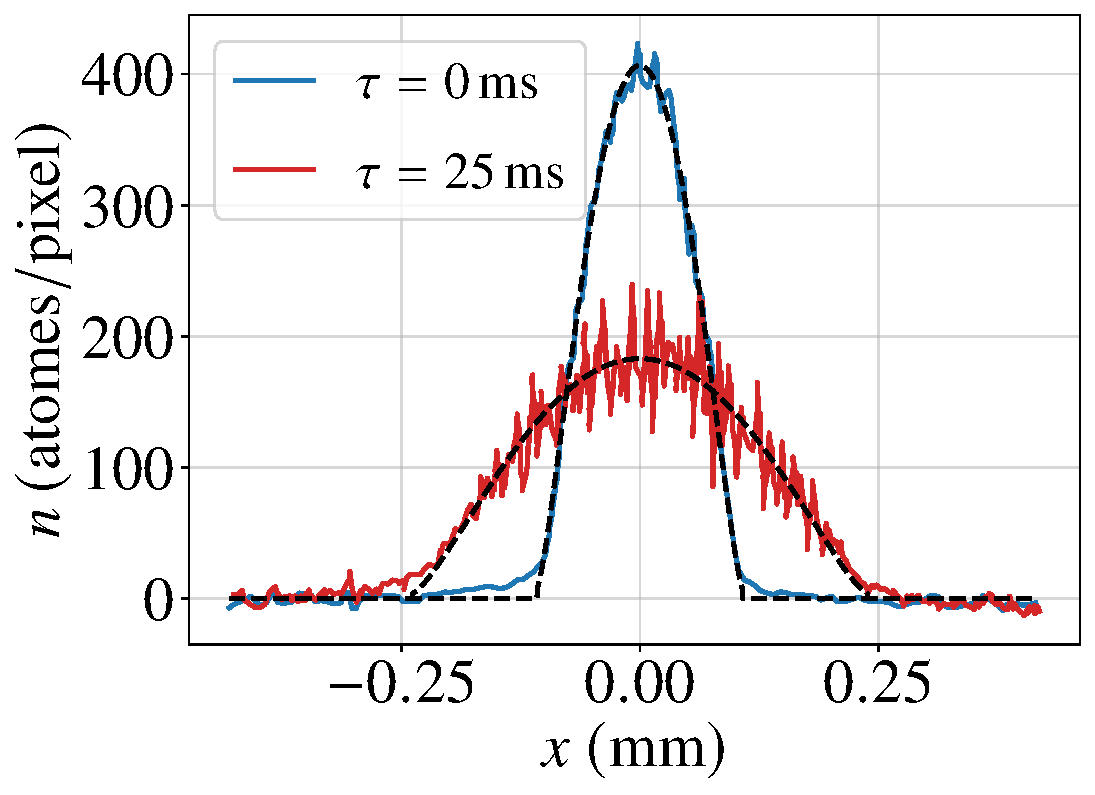
\includegraphics[width=0.45\textwidth]{./figures/05_Disp_Exp/fit_n_vs_tau.pdf}};
        	\node[above=-0.2cm of a , shift={(-2 , 0)}] {(a)};	
        \end{scope}

        
        
        % Deuxième figure
        \begin{scope}[shift={(7,0)}]
        	\node (b) at (0,0) {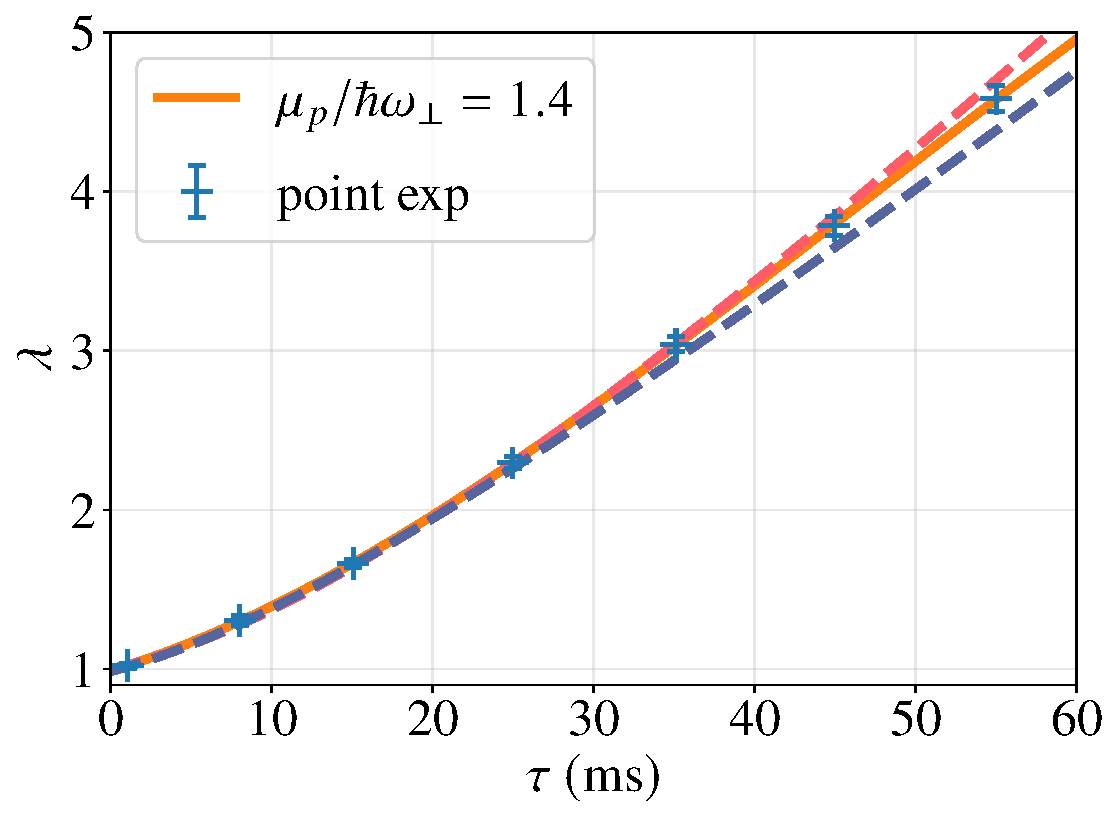
\includegraphics[width=0.45\textwidth]{./figures/05_Disp_Exp/fit_lambda_vs_tau.pdf}};
        	\node[above=-0.2cm of b , shift={(-2 , 0)}] {(b)};
        	
        	\draw[thick, color=colorSix, line width = 0.5ex , <-]
    			(1,1) to[out=180, in=90] (-2,-0.)
    			node[below, color = colorSix] { \color{\colorSix} \small TF 3D : $\mu_p \gg \hbar \omega_\perp$};	
    		\draw[thick, color=colorFour, line width = 0.5ex , <-]
    			(1.9,1) to[out=-90, in=90] (2,-0.5)
    			node[below, color = colorFour] { \color{\colorFour} \small TF 3D : $\mu_p \gg \hbar \omega_\perp$};	
        \end{scope}

        
	\end{tikzpicture}
	\caption{
(a) Profil de densité à l'équilibre dans le piège harmonique longitudinal (bleu), ajusté par $n_0(x)$ selon Eq.~\eqref{chap:eq:ajust} (noir pointillé). La courbe rouge montre le profil après une expansion longitudinale $\tau = 25~\mathrm{ms}$, avec un facteur d'échelle $\lambda$ extrait en ajustant le profil par une courbe homothétique à la densité initiale (noir pointillé), cf. Eq.~\eqref{chap:5:eq.hydro.1.3}.  
(b) Points bleus : facteurs d'échelle $\lambda(\tau)$ extraits expérimentalement. Courbe orange : résultats numériques obtenus en résolvant les équations hydrodynamiques (Eq.~\eqref{chap4:eq.pot.s.1}) avec $\mu_p / \hbar \omega_\perp = 1.4$. Les courbes pointillées montrent les évolutions attendues de $\lambda$ en résolvant Eq.~\eqref{chap:5:eq.hydro.3.4} pour $\alpha = 1$ (TF 1D) et $\alpha = 1/2$ (TF 3D).
}

	\label{fig:profil}
\end{figure}



% --- Table révisée (petites corrections typographiques) ---
%\begin{table}[h]
%\centering
%\begin{tabular}{l c c c}
%\hline
%Système & loi pour $\mu(n)$ & $\beta$ (avec $f(\lambda)=\lambda^{-\beta}$) & $\displaystyle \omega_{\rm breath}/\omega_\parallel$ \\
%\hline
%Gaz classique isotherme (1D, $\mu\propto\ln n$) 
%& $\mu'(n)\propto 1/n$ 
%& $-1$ 
%& $\sqrt{3}\approx1.732$ \\[4pt]
%
%Gaz de Bose 1D en régime moyen (GP, $\mu\propto n$) 
%& $\alpha=1$ 
%& $0$ 
%& $2$ \\[4pt]
%
%Tonks--Girardeau (1D, $\mu\propto n^2$) 
%& $\alpha=2$ 
%& $1$ 
%& $\sqrt{5}\approx2.236$ \\[4pt]
%
%Gaz de Fermi unitaire (ex. 3D, $\mu\propto n^{2/3}$) 
%& $\alpha=\tfrac{2}{3}$ 
%& $-\tfrac{1}{3}$ 
%& $\sqrt{3+\tfrac{2}{3}}\approx1.915$ \\[4pt]
%
%Cas général (loi de puissance) 
%& $\mu\propto n^\alpha$ 
%& $\beta=\alpha-1$ 
%& $\displaystyle \sqrt{3+\alpha}$ \\
%\hline
%\end{tabular}
%\caption{Valeurs de $\beta$ et fréquences du mode de souffle pour quelques régimes usuels.}
%\label{tab:breathing}
%\end{table}
% 



\subsection{Sonde locale de distribution de rapidité}


\subsubsection{Distribution de rapidités locale dans les gaz 1D}

%\paragraph{Motivation.}  
%La compréhension des gaz de bosons 1D avec interactions de contact répulsives repose sur la notion de distribution de rapidités \(\rho(\theta)\). Chaque état propre du système peut être paramétré par un ensemble de rapidités \(\{\theta_i\}\) , ou interprété comme les vitesses de quasi-particules à durée de vie infinie. Ici, on utilise la définition pratique issue des expansions 1D : les rapidités correspondent aux vitesses asymptotiques des atomes après une expansion, avec \(x_j \simeq \tau \theta_j\) pour un temps \(\tau\) long \footnote{Dans une article \cite{bezzaz2023rapiditydistributiondefocusingnonlinear} on voit que La limite champ classique du gaz de Lieb Liniger correspond à l’Équation de
%Schrödinger Non-Linéaire. Dans ce cadre, la théorie de diffusion inverse permet
%de construire un ensemble de quantités conservées.
%— Une méthode permettant de faire le lien entre la distribution de rapidité et
%les quantités conservées issues de la théorie de diffusion inverse est d’utiliser
%la définition de la distribution de rapidités comme distribution en impulsion
%asymptotique des atomes après une expansion 1D. On retrouve alors un résultat
%connu. J'ai bien cette aproche avec l'inverse scatering }. 
%\begin{eqnarray*}
%	\tilde{n}(v , \tau ) \underset{\tau \to \infty}{\rightarrow} \Pi (v).
%\end{eqnarray*}
%Cette définition est directement applicable à des mesures expérimentales de distribution de rapidités locales car à temps long la distribution spatial devient homotétique à la distribution de vitestes $\tau n (x , \tau ) \underset{\tau \to \infty}{\rightarrow} n (x/\tau , \tau) $ soit 
%\begin{eqnarray*}
%	\tau n (x , \tau )	 \underset{\tau \to \infty}{\rightarrow} \Pi (x/\tau).
%\end{eqnarray*}

\paragraph{Motivation.}  
La compréhension des gaz de bosons unidimensionnels avec interactions de contact répulsives repose sur la notion de distribution de rapidités \(\rho(\theta)\). Chaque état propre du système peut être caractérisé par un ensemble de rapidités \(\{\theta_i\}\), interprétées comme les vitesses de quasi-particules à durée de vie infinie.  

Dans le cadre des expansions 1D, une définition pratique consiste à assimiler les rapidités aux vitesses asymptotiques des atomes après une expansion libre, via la relation \(x_j \simeq \tau \theta_j\) pour un temps d’expansion long \(\tau\) \footnote{Dans la limite champ classique, le gaz de Lieb–Liniger est décrit par l’équation de Schrödinger non-linéaire. La théorie de diffusion inverse permet alors de construire un ensemble de quantités conservées. Dans ce cadre, la distribution de rapidités peut être définie comme la distribution en impulsion asymptotique des atomes après une expansion 1D, ce qui établit un lien direct entre rapidités et quantités conservées \cite{bezzaz2023rapiditydistributiondefocusingnonlinear}}.
.  

Ainsi, la distribution de vitesses mesurée à long temps tend vers la distribution de rapidités \(\Pi(v)\) :  
\[
	\tilde{n}(v , \tau ) \underset{\tau \to \infty}{\longrightarrow} \Pi(v).
\]  
Cette définition est directement exploitable expérimentalement : à temps long, la distribution spatiale devient homothétique à la distribution de vitesses,  
\[
	\tau n(x , \tau ) \underset{\tau \to \infty}{\longrightarrow} \Pi(x/\tau).
\] 


\paragraph{Distribution locale et LDA.}  
Pour un nuage atomique piégé dans un potentiel longitudinal variant lentement, on peut appliquer la \gls{LDA}. Le gaz est alors vu comme un fluide décomposé en cellules mésoscopiques de densité homogène et relaxée. Dans chaque cellule, l’état d’équilibre est décrit par un \gls{GGE}, ou équivalemment par une distribution de rapidités locale \(\rho(x,\theta)\). Cette description permet d’étudier non seulement l’équilibre, mais aussi la dynamique hors équilibre à grandes échelles spatiales et temporelles, via la théorie \gls{GHD}.

\paragraph{Protocole expérimental.}  
Pour mesurer \(\rho(x,\theta)\) localement :  
\begin{enumerate}
    \item Une zone du nuage atomique de taille \(\ell\) centrée en \(x_0\) est sélectionnée à l’aide du \gls{DMD}. La pression de radiation supprime instantanément les atomes en dehors de la zone, laissant uniquement ceux de la cellule (Fig ~\ref{fig:selection}).
    \item Après la sélection, le confinement longitudinal est relâché, tandis que le confinement transverse reste actif. Les atomes réalisent une expansion 1D pendant un temps \(\tau\), puis le profil de densité est imagé (typiquement pour \(\tau\sim 60\) ms).
    \item Le protocole est répété pour plusieurs positions \(x_0\), permettant d’obtenir la distribution de rapidités locale sur l’ensemble du nuage.
\end{enumerate}

\begin{figure}[H]
	\centering
	\begin{tikzpicture}
		%\begin{scope}[transform canvas={scale=0.6}]
	
		\begin{scope}[shift={(0,0)}]
			
		


        \begin{scope}[shift={(0,0)}, transform canvas={scale=0.5}]
        	\draw[thick, color = \colorFour , fill = \colorFour,line width = 0.5ex ] (0,0) ellipse [x radius=4cm, y radius=0.2cm];
        	\draw 
        		(-5 , 0 ) edge[thick, color=colorOne, line width = 0.5ex , ->] node[pos = 1.0 ,   below , color = \colorOne]{\fontsize{18}{20}\selectfont  $x$}  (5,0)
        		(0,-1) edge[thick, color=colorOne, line width = 0.5ex , ->] node[pos = 1.0 , left , color = \colorOne]{\fontsize{18}{20}\selectfont  $y$} (0,1)
        		
        		(1,-0.3) edge[thick, color=colorThree, line width = 0.4ex ] node[pos = 0.0 , below , color = \colorThree]{\fontsize{18}{20}\selectfont  $x_0$} (1,0.3)
        		
        		(-0.5,0) edge[shift = {(1,0.45)} , thick, color=colorThree, line width = 0.4ex , <->] node[pos = 0.5 , above , color = \colorThree]{\fontsize{18}{20}\selectfont  $\ell$} (0.5,0)
        		
        		(0,0) edge[shift = {(-3,0.5)} , thick, color=colorOne, line width = 0.4ex , <-] node[shift = {(0,-0.1)} , pos = 1 , above , color = \colorOne]{\fontsize{15}{20}\selectfont  $5\, \mu m $} (0,0.25)
        		(0,0) edge[shift = {(-3,-0.5)} , thick, color=colorOne, line width = 0.4ex , <-] (0,-0.25)
        	;
        	 % Contour
			\draw[line width=0.4ex, color=colorSix]
    			(1.5,-0.5) rectangle +(3,1)
    			(0.5,-0.5) rectangle +(-5,1);

			% Remplissage avec hachures épaisses
			\fill[pattern={Lines[angle=-45,distance={5pt},line width=0.4ex]}, pattern color=colorSix]
    			(1.5,-0.5) rectangle +(3,1)
    			(0.5,-0.5) rectangle +(-5,1);
    		
    		\draw[thick, color=colorSix, line width=0.5ex, <-]
    			(-2,-0.4) to[out=-90, in=0] (-2.4,-1.3)
   				 node[left, color=colorSix, align=left] 
    			{\fontsize{12pt}{14pt}\selectfont \bfseries \itshape
    			faisceau lumineux\\
    			\bfseries \itshape façonné par le DMD}
    		;
    		\draw[thick, color=colorFour, line width=0.5ex, <-]
    			(-1,-0.0) to[out=-90, in=-180] (1,-1.3)
   				 node[right, color=colorFour, align=left] 
    			{\fontsize{12pt}{14pt}\selectfont \bfseries \itshape
    			nuage atomique}
    		;	
        		
        \end{scope}
        \draw [color = white] (-3,-1) rectangle +(10,2);
		\node[shift={(-3 , 1)}] at (0,0) {a)};
     	\end{scope}
     	
     	 % Deuxième figure
        \begin{scope}[shift={(7,0)}]
        	\node (b) at (0,0) {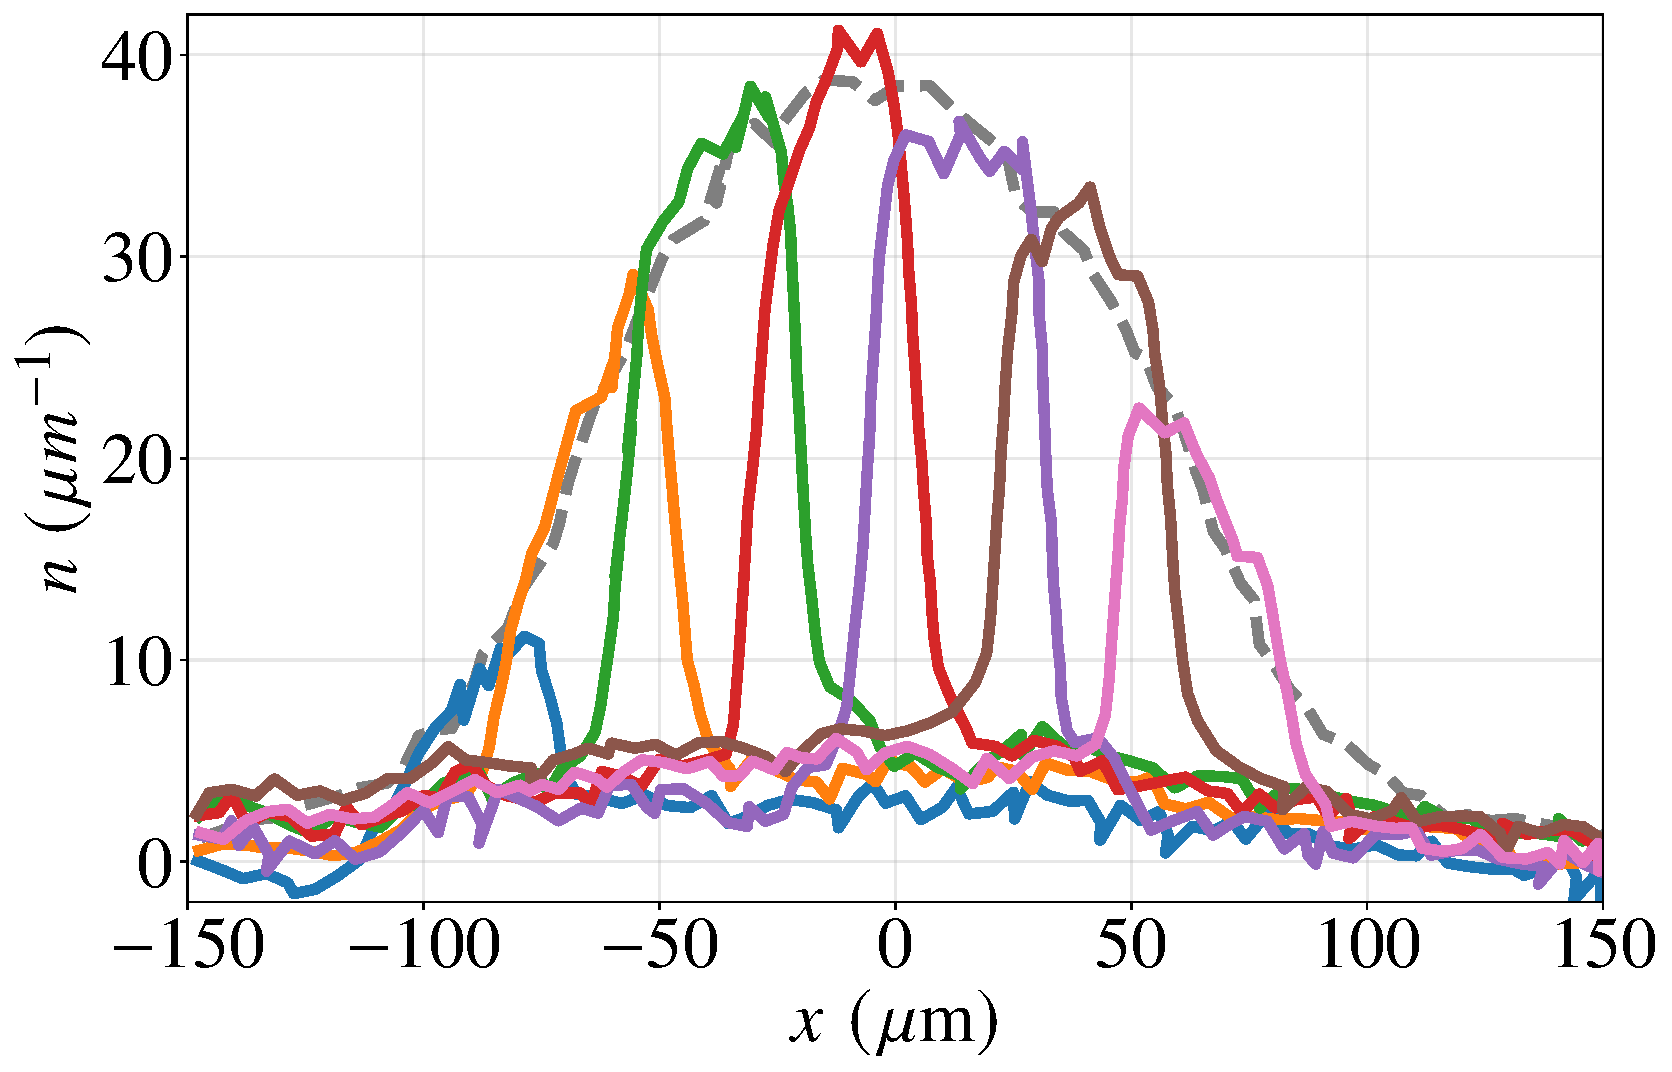
\includegraphics[width=0.55\textwidth]{./figures/05_Disp_Exp/profils.pdf}};
        	\node[above=-0.2cm of b , shift={(-2 , 0)}] {b)};
        	
%        	\draw[thick, color=colorSix, line width = 0.5ex , <-]
%    			(1,1) to[out=180, in=90] (-2,-0.)
%    			node[below, color = colorSix] { \color{\colorSix} \small TF 3D : $\mu_p \gg \hbar \omega_\perp$};	
%    		\draw[thick, color=colorFour, line width = 0.5ex , <-]
%    			(1.9,1) to[out=-90, in=90] (2,-0.5)
%    			node[below, color = colorFour] { \color{\colorFour} \small TF 3D : $\mu_p \gg \hbar \omega_\perp$};	
        \end{scope}

        
	\end{tikzpicture}
	\caption{(a) Schéma illustrant la sélection d’une région du nuage atomique, ici représentée par un ellipse bleu illuminé par un faisceau modulé à l’aide du DMD.\\
(b) Exemple de sélections sur un gaz initialement à l’équilibre : superposition du profil de densité initial du nuage (courbe grise) et des profils mesurés après $\tau = 1~\mathrm{ms}$ pour différentes régions de sélection de taille $\ell = 37~\mu\mathrm{m}$ centrées en différentes positions $x_0$ (courbes colorées).
}

	\label{fig:selection}
\end{figure}

\paragraph{Mesures à l’équilibre.}  
Pour un gaz initialement à l’équilibre dans un piège harmonique, le profil de densité de chaque zone sélectionnée est analysé via \gls{TBA} et la \gls{LDA}, donnant température \(T\) et potentiel chimique \(\mu\). Après un temps d’expansion long, le profil devient homothétique à la distribution de rapidités locale \(\rho(x,\theta)\). La comparaison avec les prédictions numériques montre une bonne cohérence, confirmant que le protocole permet de sonder efficacement \(\rho(x,\theta)\).


\begin{figure}[H]
	\centering
	\begin{tikzpicture}
		%\begin{scope}[transform canvas={scale=0.6}]
	
		\begin{scope}[shift={(0,0)}]
			
			\node (a) at (0,0) {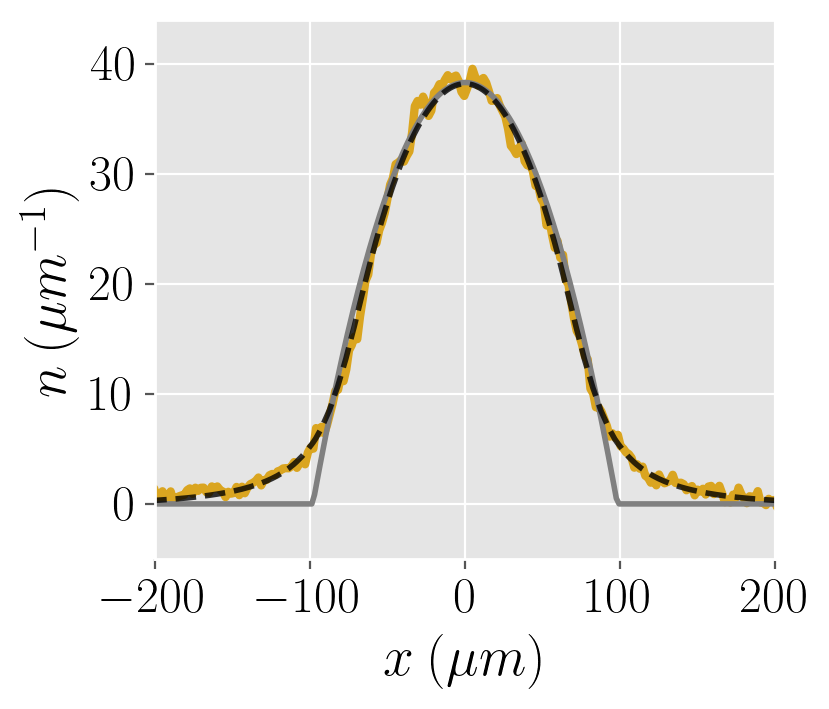
\includegraphics[width=0.3\textwidth]{./figures/05_Disp_Exp/image159.png}};
        	\node[above=-0.2cm of a , shift={(-2 , 0)}] {a)};


                
        %\draw [color = white] (-3,-1) rectangle +(10,2);

     	\end{scope}
     	
     	 % Deuxième figure
        \begin{scope}[shift={(7,0)}]
        	\node (b) at (0,0) {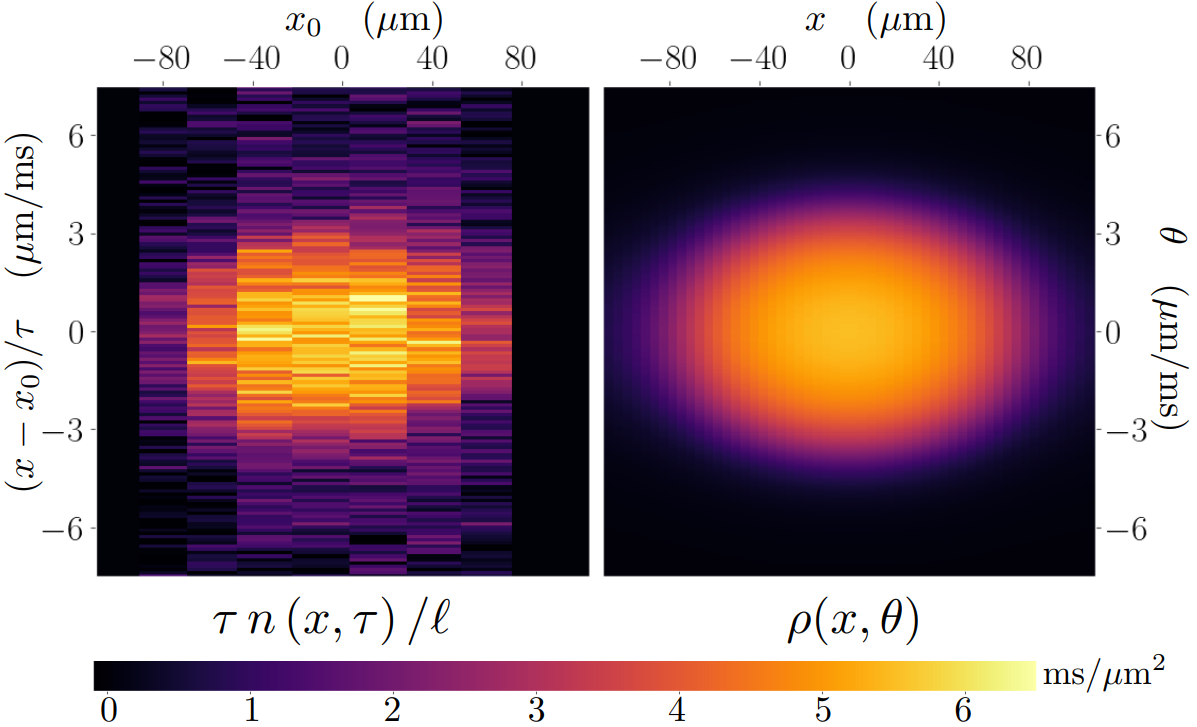
\includegraphics[width=0.6\textwidth]{./figures/05_Disp_Exp/image212.png}};
        	\node[above=-0.2cm of b , shift={(-3.2 , -1.3)} , color = white ] {\color{white} b1)};
        	\node[above=-0.2cm of b , shift={(0.5 , -1.3)} , color = white ] {\color{white} b2)};
        	
        \end{scope}

        
	\end{tikzpicture}
	\caption{a) Profil de densité d’un nuage atomique initialement à l’équilibre dans un piège harmonique avec $\omega_\perp = 2 \pi \times  2.6~\mathrm{kHz}$ et $\omega_\parallel = 2 \pi \times 5~\mathrm{Hz}$ (zone en jaune). La courbe grise représente le profil parabolique attendu à l’état fondamental dans le régime qBEC, décrit par l’équation d’état $n(x) = [\mu - V_\parallel(x)]/g$. La courbe noire en pointillés correspond à un ajustement des données expérimentales en supposant que le système soit bien décrit par un ensemble thermique (\gls{TBA} (Sec ~ \ref{chap4:sec:TBA})). Cet ajustement permet d’extraire une température $T = 90~\mathrm{nK}$ et un potentiel chimique $\mu/k_B = 49~\mathrm{nK}$.
	(b1) Profils de densités pour différents centres de sélection x0 représentés sur la Fig.\ref{fig:selection}(b). Les sélections sont de taille $\ell = 37\, \mu m$ et les profils obtenus après un temps d’expansion $\tau =  40 \, ms$. Pour comparer les résultats à une distribution de rapidités, les profils de densités sont multipliés par le rapport $\tau/ \ell$ et sont tracés en fonction de $(x-x_0)/\tau$ (b2). (b2) Prédiction théorique de la distribution de rapidités spatialement résolue $\rho ( x , \theta)$ à l’équilibre thermique dans un potentiel harmonique longitudinal avec $\omega_\parallel = 2 \pi \times 5~\mathrm{Hz}$. La température $T$ et le potentiel chimique $\mu$ utilisés sont eux obtenus à partir du profil in situ (a).}
	\label{fig:expansion}
\end{figure}

\paragraph{Résumé.}  
— Une sonde locale de distribution de rapidités a été mise en place grâce au \gls{DMD}.  
— Les atomes sélectionnés réalisent une expansion dans le guide 1D.  
— Après un temps long, le profil de densité reflète la distribution de rapidités locale.  
— Ce protocole a été appliqué avec succès sur un nuage atomique initialement à l’équilibre.

\paragraph{Dynamique.}
\subparagraph{Motivation.}
Pour vérifier si le régime asymptotique des expansions longitudinales est atteint, il est nécessaire de comparer les résultats expérimentaux à une théorie dynamique. L’outil adapté est de \gls{GHD}, déjà introduite au Chapitre~\ref{chap:GHD}, qui décrit l’évolution spatio-temporelle de la distribution de rapidités.

\subparagraph{Invariance d’échelle hydrodynamique.}
On considère une sélection initiale homogène de taille $\ell$ centrée en $x_0$. Dans ce cas, les équations \gls{GHD} \eqref{chap:GHD:eq.conserv.3.1} s’écrivent sans potentiel, avec la condition initiale $\rho(x,\theta,0)=\rho_0(\theta)$ si $|x-x_0|\leq \ell/2$, et $0$ sinon. En introduisant les variables sans dimension $\alpha=(x-x_0)/\ell$ et $\beta=\tau/\ell$, l’équation devient indépendante de $\ell$. 
\begin{eqnarray*}
	\left \{ 
	\begin{array}{rcl}
		\partial_\beta \tilde{\rho} ( \alpha , \theta ; \beta ) +  \partial_x ( v^{\mathrm{ell}}_{[\tilde{\rho}]} (\theta)  \tilde{\rho} ( \alpha , \theta ; \beta )) = 0 \\
		\tilde{\rho} ( \alpha , \theta ; 0 )	 = \begin{cases}
			\rho_0(\theta) & \text{si } |\alpha|\leq \tfrac{1}{2}, \\
			0 & \text{sinon},
		\end{cases}% \rho_0(\theta) \, \mbox{si} \, \vert \alpha \vert \leq \frac12 \,, \,  0 \, \mbox{sinon}.
	\end{array}
	\right .
\end{eqnarray*}
Il en résulte que les profils de densité $n(x,\tau)$, exprimés en fonction de $\alpha$, ne dépendent que du rapport $\beta$. 
Autrement dit, deux sélections de tailles différentes mais telles que $\tau/\ell$ soit constant doivent conduire aux mêmes profils après expansion. Cette invariance a été vérifiée expérimentalement : les profils se superposent de manière remarquable (Fig ~\ref{fig:scail2} a)) .

\subparagraph{Lien avec les équations de Gross–Pitaevskii}
Dans le régime \gls{qBEC}, à basse température, la dynamique peut aussi être décrite par les équations hydrodynamiques issues de \gls{GP} (en négligeant la pression quantique) 
Après changement de variables ($\alpha=(x-x_0)/\ell$, $\beta=\tau/\ell$, $\tilde n=n/n_0$), on retrouve un système d’équations qui ne dépend plus de $\ell$, mais uniquement du rapport adimensionné $\eta=\beta g n_0/m$.
\begin{eqnarray*}
	\left \{ 
	\begin{array}{rcl}
		\partial_\beta \tilde n + \partial_\alpha ( \tilde v \tilde n) = 0, && \partial_\beta \tilde v + \tilde v \,\partial_\alpha \tilde v = - \dfrac{g n_0}{m}\,\partial_\alpha \tilde n, \\[6pt]
	\tilde n(\alpha,\beta=0) = 
		\begin{cases}
			1 & \text{si } |\alpha|\leq \tfrac{1}{2}, \\
			0 & \text{sinon},
		\end{cases}, && 
\tilde v(\alpha,\beta=0)=0.
	\end{array}
	\right.
\end{eqnarray*}
Il en découle que les profils de densité sont universels lorsqu’ils sont exprimés en fonction de $(\alpha,\eta)$. Expérimentalement, ce comportement est bien confirmé : les centres des profils se superposent pour des conditions initiales différentes, et l’accord est même bon sur les bords (Fig ~\ref{fig:scail2} b)) .

\begin{figure}[H]
	\centering
	\begin{tikzpicture}
		%\begin{scope}[transform canvas={scale=0.6}]
	
		\begin{scope}[shift={(0,0)}]
			
			\node (a) at (0,0) {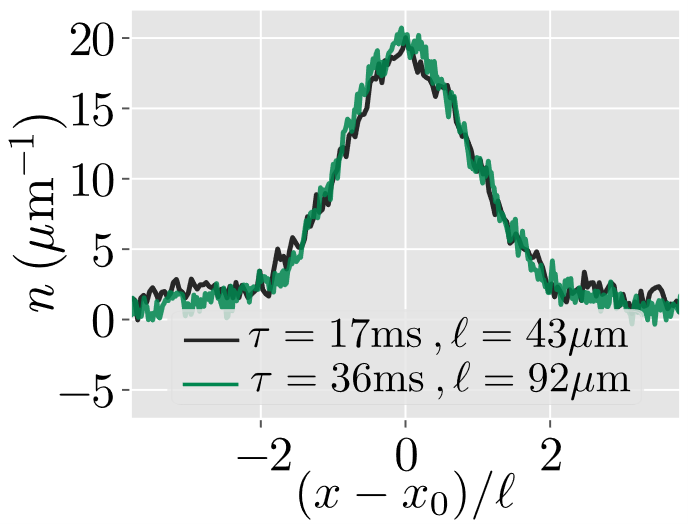
\includegraphics[width=0.5\textwidth]{./figures/05_Disp_Exp/image246.png}};
        	\node[above=-0.2cm of a , shift={(-2 , -1)}] {\color{black} a)};


                
        %\draw [color = white] (-3,-1) rectangle +(10,2);

     	\end{scope}
     	
     	 % Deuxième figure
        \begin{scope}[shift={(7,0)}]
        	\node (b) at (0,0) {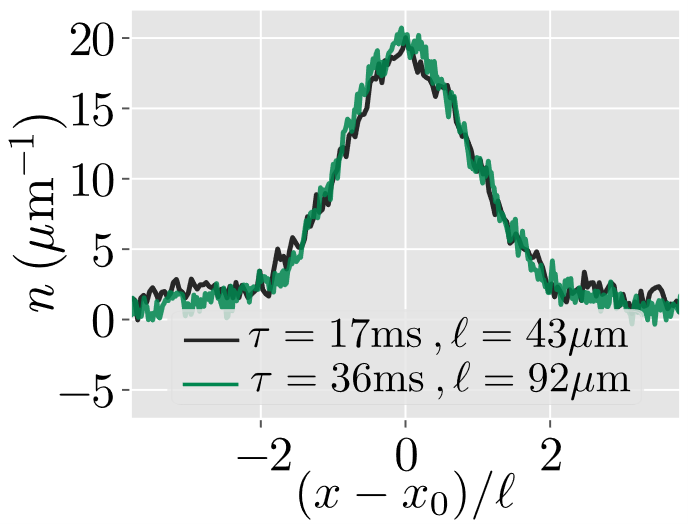
\includegraphics[width=0.5\textwidth]{./figures/05_Disp_Exp/image246.png}};
        	\node[above=-0.2cm of b , shift={(-2 , -1.)} ] {\color{black} b)};
        	
        	
        \end{scope}

        
	\end{tikzpicture}
	\caption{(a) Illustration du comportement hydrodynamique prédit par les équations de GHD. Deux profils de densité sont représentés en fonction de $\alpha$ pour un même paramètre $\beta = \tau / \ell = 0.39~\mathrm{ms}/\mu\mathrm{m}$.(b) Analyse du comportement hydrodynamique selon le formalisme GP. Deux profils de densité sont tracés pour un même ratio $\eta = (\tau/\ell)\, g n_0 / m = 2.65$, avec une taille de sélection $\ell = 37~\mu\mathrm{m}$, mais pour des densités initiales $n_0$ différentes. Les sélections ont été réalisées sur plusieurs régions distinctes d’un même nuage.
	}

	\label{fig:scail2}
\end{figure}

\subparagraph{Régime asymptotique.}  
L’expansion des tranches est bien décrite par \gls{GHD}. Les comparaisons entre données expérimentales et simulations \gls{GHD} (avec des distributions thermiques initiales) montrent un bon accord au centre des profils, mais révèlent que le régime asymptotique complet n’est pas atteint dans les temps accessibles expérimentalement. On définie un écart-type $$\sigma(\tau) = \sqrt{ \frac{\int \vert \frac{\tau}{\ell} n_{\mathrm{GHD}}( \frac{x-x_0}\tau) - \rho(\frac{x-x_0}\tau) \vert^2 d \tau }{ \int \vert \rho( \frac{x-x_0}\tau) \vert^2 d \tau} }$$ avec $n_{\mathrm{GHD}}$ les profil tirés des simulations \gls*{GHD}.Pour $\tau=50$\,ms, l’écart-type reste d’environ $12\%$, et une convergence complète nécessiterait des temps irréalistes ($\sim 500$\,ms). L’extraction de la distribution de rapidité à partir des profils reste donc approximative.

\begin{figure}[H]
	\centering
	\begin{tikzpicture}
		%\begin{scope}[transform canvas={scale=0.6}]
	
		\begin{scope}[shift={(0,0)}]
			
			\node (a) at (0,0) {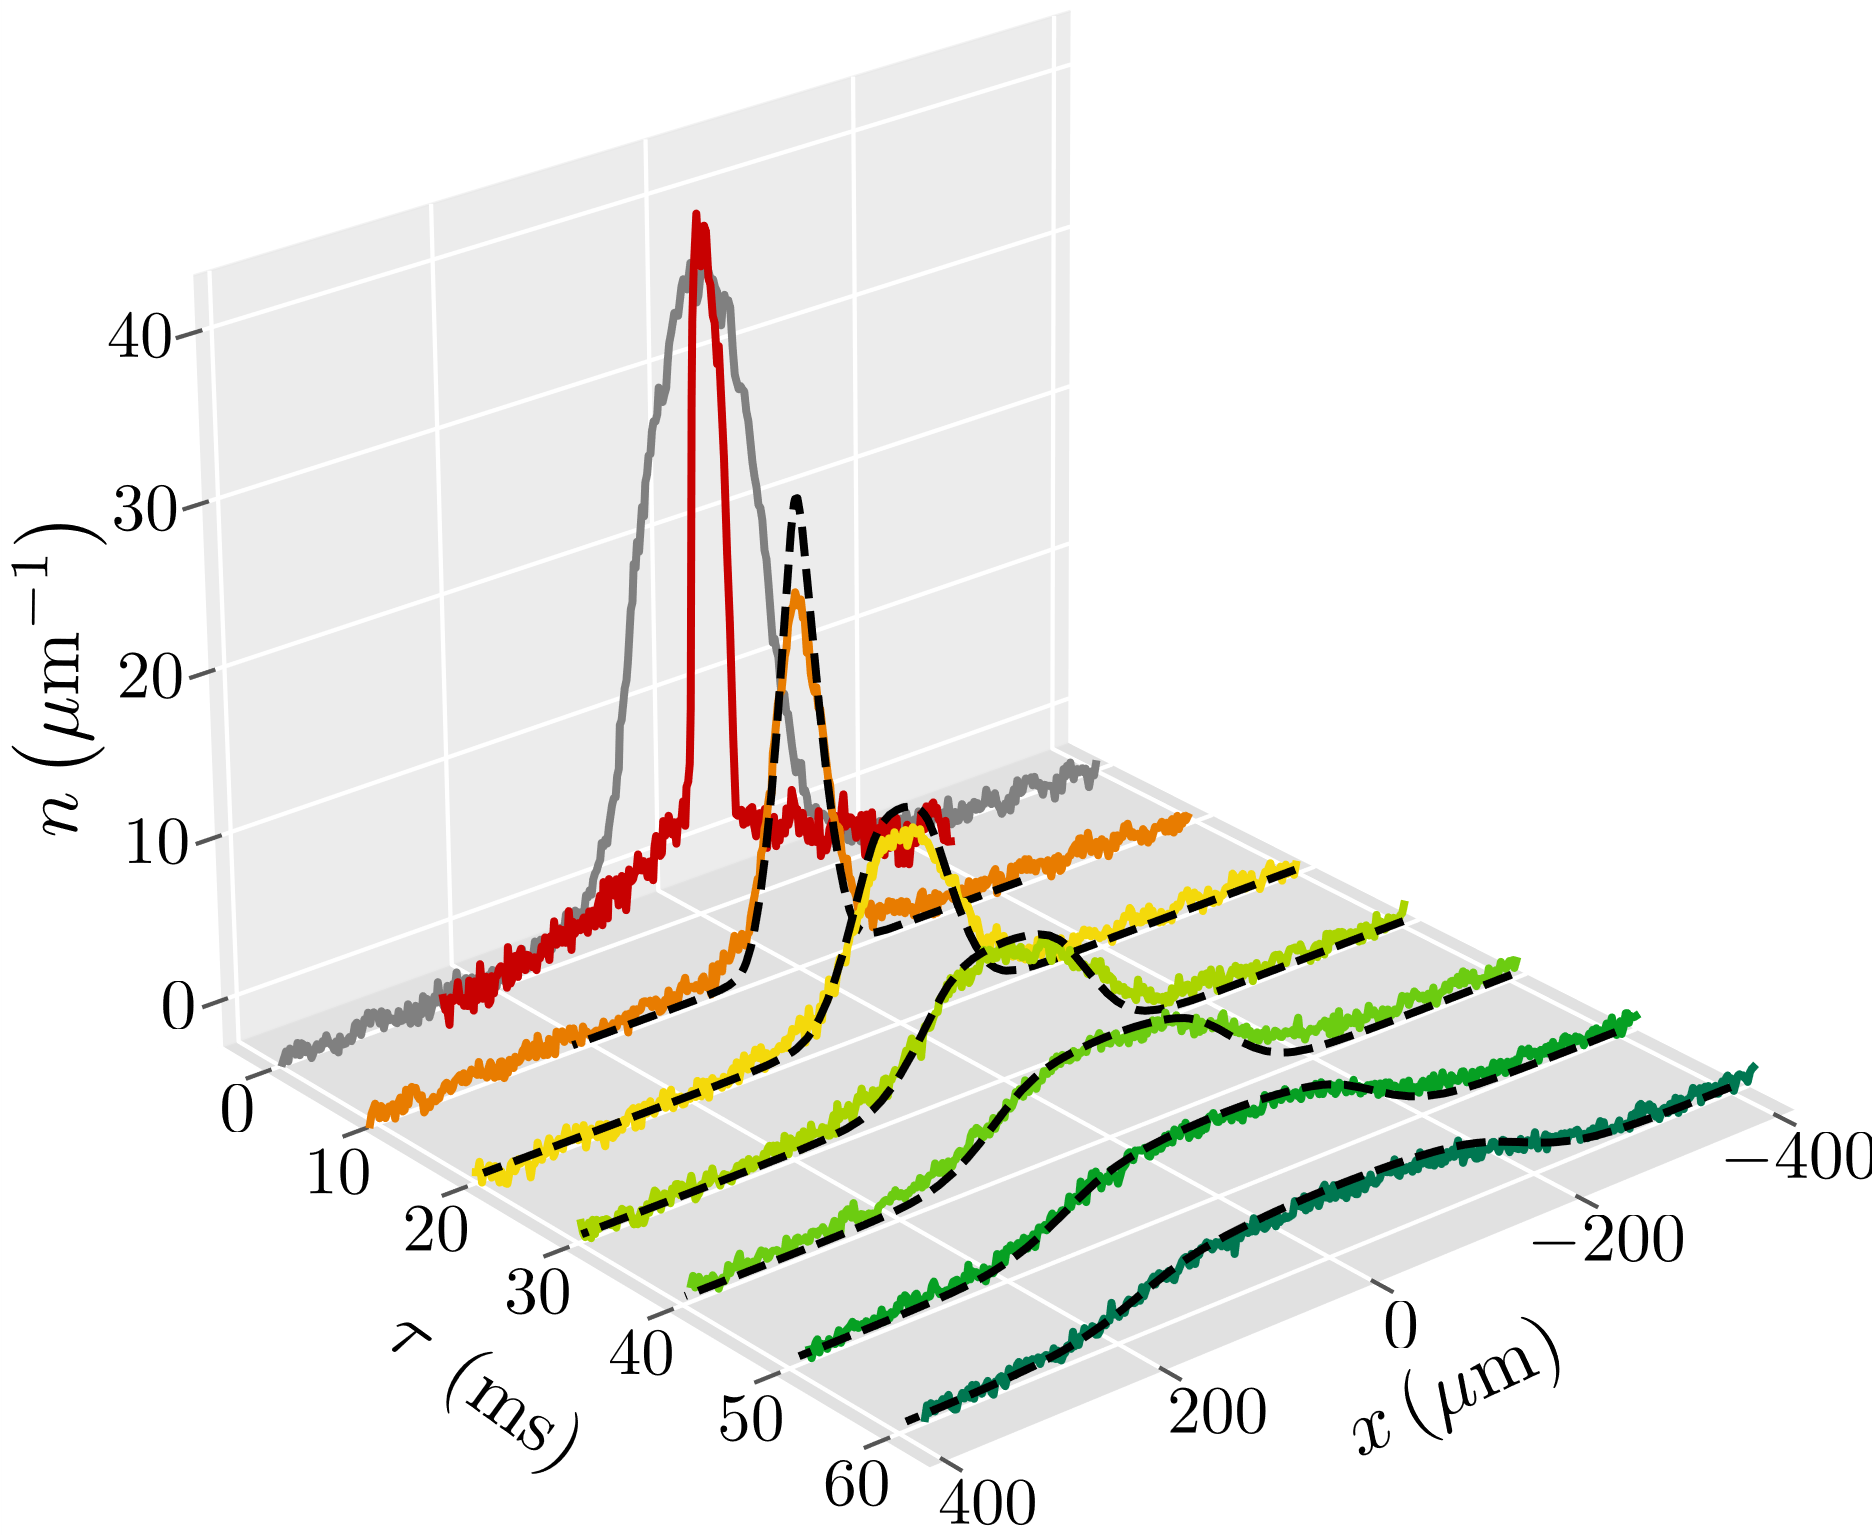
\includegraphics[width=0.7\textwidth]{./figures/05_Disp_Exp/image255.png}};
        	\node[above=-0.2cm of a , shift={(-2 , -1)}] {\color{black} a)};


                
        %\draw [color = white] (-3,-1) rectangle +(10,2);

     	\end{scope}
     	
     	 % Deuxième figure
        \begin{scope}[shift={(7,0)}]
        	\node (b) at (0,0) {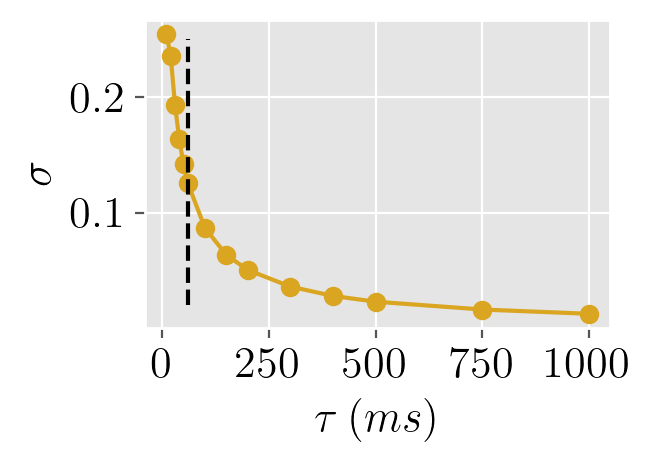
\includegraphics[width=0.3\textwidth]{./figures/05_Disp_Exp/image265.png}};
        	\node[above=-0.2cm of b , shift={(-2 , -1.)} ] {\color{black} b)};
        	
        	
        \end{scope}

        
	\end{tikzpicture}
	\caption{(a) La tranche , centrée en $x_0 = 0\,\mu\mathrm{m}$ ,subit une expansion le long de l'axe longitudinalet d'une largeur $\ell = 37\,\mu\mathrm{m}$. Le profil initial du gaz est montré en gris. Les variations de densité pour différents temps d'expansion sont représentées par des courbes colorées. Les lignes pointillées noires indiquent les résultats des simulations GHD pour une distribution de rapidités initialement thermique, paramétrée par la température $T$ et le potentiel chimique $\mu(x_0)  = \mu$, tels qu'ils sont extraits du profil de densité in situ.(b) L'écart-type $\sigma(\tau) = \sqrt{ \int \vert \frac{\tau}{\ell} n _{\mathrm{GHD}}( (x-x_0)/\tau) - \rho( (x-x_0)/\tau) \vert^2 d \tau / \int \vert \rho( (x-x_0)/\tau) \vert^2 d \tau } $ défini par l'équation~(8.8) est calculé entre la distribution de rapidités et les résultats des simulations GHD en fonction du temps d'expansion $\tau$. La ligne verticale noire correspond au temps d'expansion utilisé dans l'expérience.
}

	\label{fig:GHD1}
\end{figure}

%\subparagraph{Hypothèse thermique.}  
%Afin de restreindre le nombre de paramètres d’ajustement, on suppose que la distribution de rapidité locale est thermique. Dans ce cas, seule la température $T$ est ajustée, le potentiel chimique étant fixé par l’équation d’état. L’ajustement sur les profils expérimentaux conduit à une température effective $T_{\text{fit}}=230$\,nK, environ 2.5 fois plus grande que celle extraite à l’équilibre. Néanmoins, les distributions de rapidité obtenues restent proches, confirmant que, dans le régime fortement \gls{qBEC}, la dynamique dépend surtout des interactions et peu de la température. L’influence possible d’une faible population transversale excitée a été évaluée et s’est révélée négligeable.

\subsection*{8.6 Mesure locale de distribution de rapidités hors équilibre}

\paragraph{Mise en place d’une distribution locale hors équilibre.}  
Le faisceau de sélection (\gls{DMD}) permet non seulement de sonder la distribution de rapidités locale, mais aussi de créer des situations hors équilibre. Un protocole illustratif consiste à retirer les atomes d’une région centrale de taille $\ell_0 = 70\,\mu$m, puis à laisser le gaz évoluer librement longidutalement (1D). Après un temps $\tau = 15$\,ms, la distribution de rapidités développe une structure doublement piquée, très différente d’une distribution thermique. Une seconde sélection locale ($\ell=35\,\mu$m) suivie d’une expansion révèle expérimentalement ce profil, en excellent accord avec les simulations GHD (Fif ~\ref{fig:GHD2}).

\begin{figure}[H]
	\centering
	\begin{tikzpicture}
		%\begin{scope}[transform canvas={scale=0.6}]
	
		\begin{scope}[shift={(0,0)}]
			
			\node (a) at (0,0) {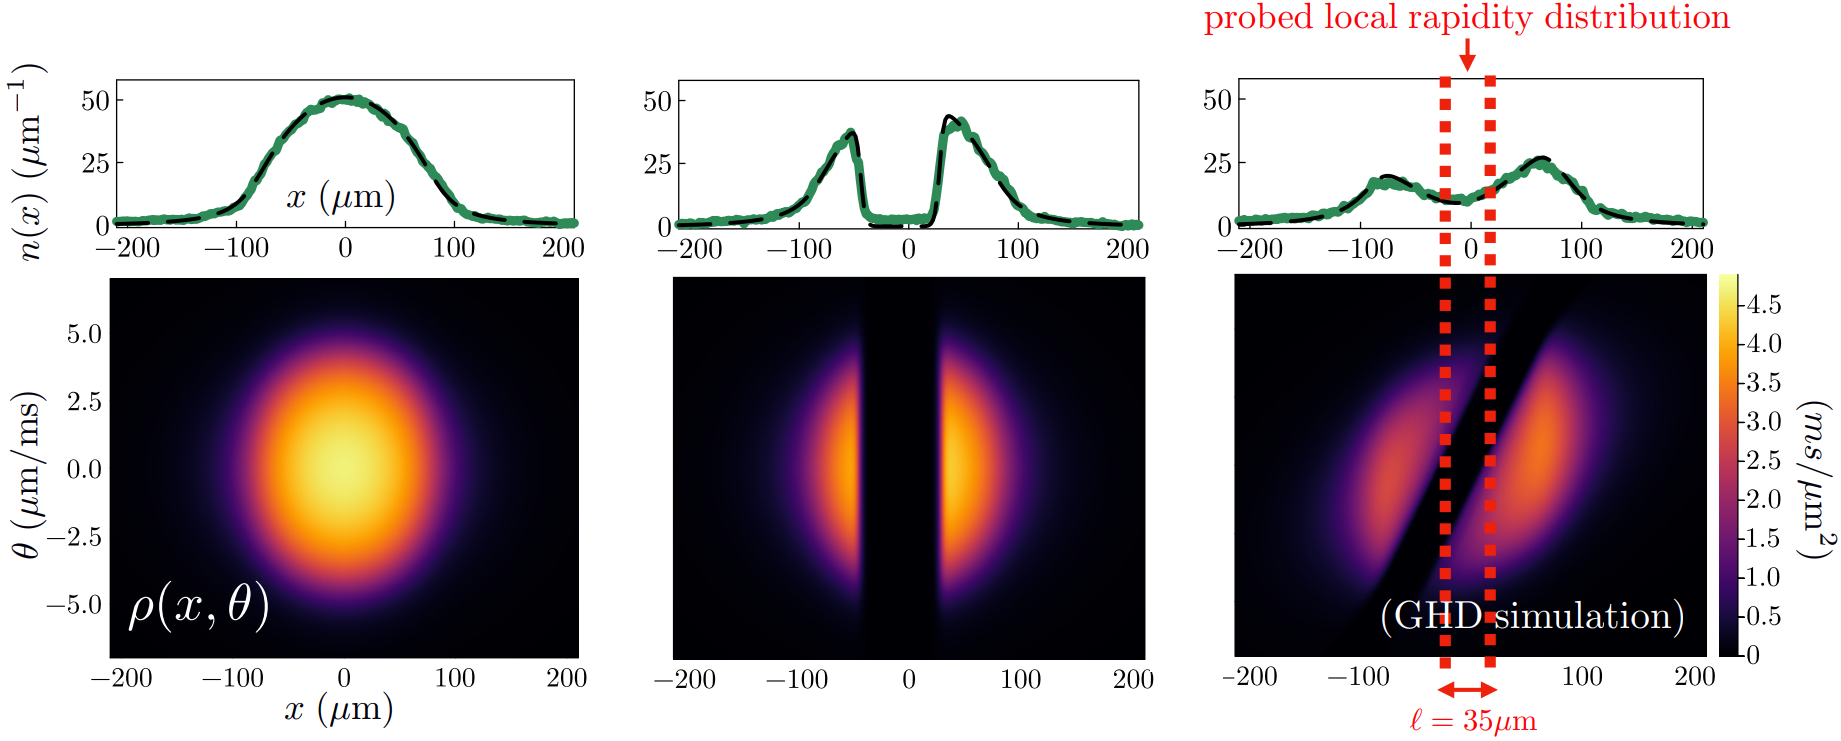
\includegraphics[width=0.6\textwidth]{./figures/05_Disp_Exp/image295.png}};
        	\node[above=-0.2cm of a , shift={(-2 , -1)}] {\color{black} a)};


                
        %\draw [color = white] (-3,-1) rectangle +(10,2);

     	\end{scope}
     	
     	 % Deuxième figure
        \begin{scope}[shift={(7,0)}]
        	\node (b) at (0,0) {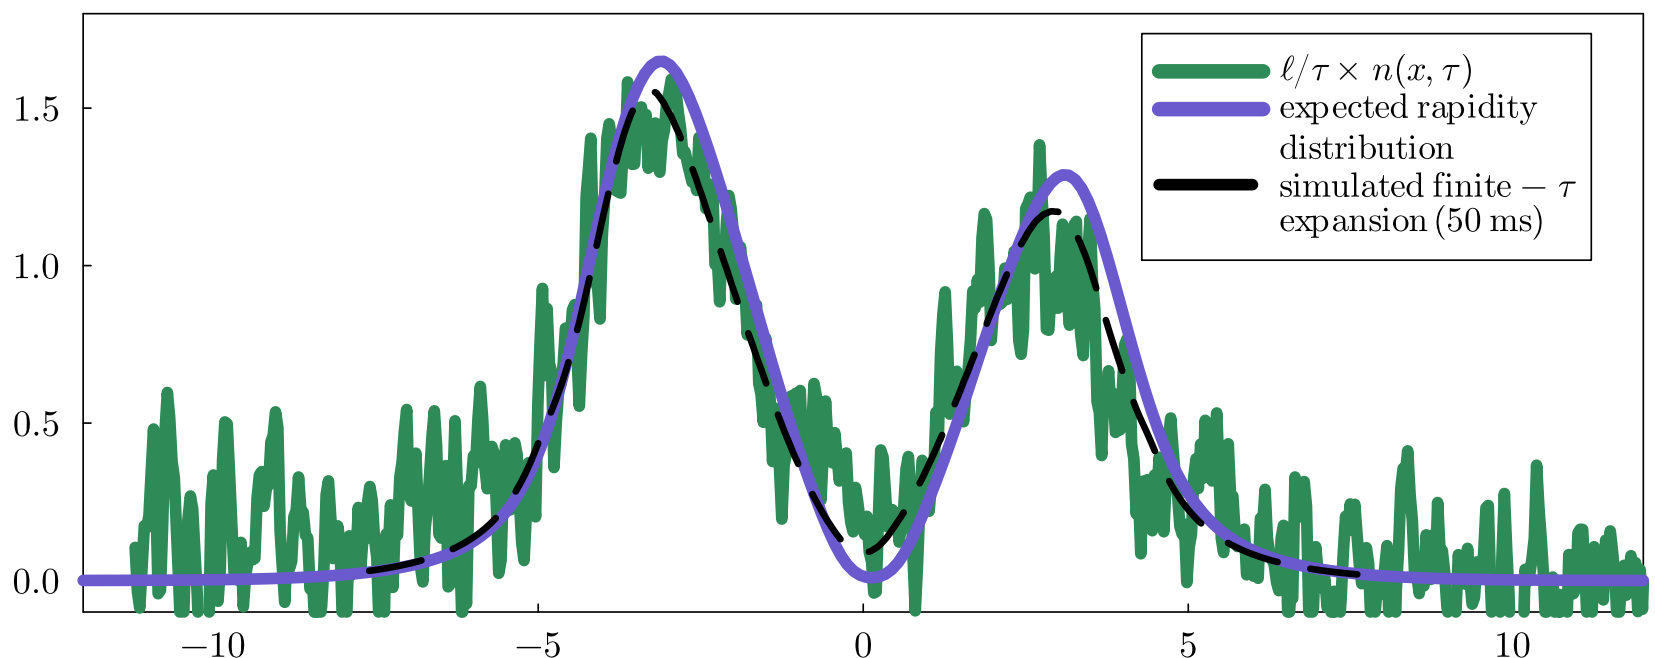
\includegraphics[width=0.4\textwidth]{./figures/05_Disp_Exp/image290.png}};
        	\node[above=-0.2cm of b , shift={(-2 , -1.)} ] {\color{black} b)};
        	
        	
        \end{scope}

        
	\end{tikzpicture}
	\caption{Les profils de densité sont montrés à différents stades : à l'équilibre initial (a1), 1\,ms après la première sélection (a2), et 15\,ms après une expansion le long du guide 1D (a3). Les distributions de rapidités résolues spatialement correspondantes sont illustrées dans les panels (a4) à (a6). Les lignes pointillées rouges indiquent la deuxième sélection.  (b)Pour obtenir la distribution locale de rapidités, on trace $\tau\, n(x,\tau)/\ell$ sur une région de largeur $\ell = 36\,\mu\mathrm{m}$ après un temps d'expansion longitudinal $\tau = 50\,\mathrm{ms}$. Le profil présente une double crête et montre un excellent accord avec la prédiction théorique de la distribution de rapidités (courbe violette), y compris les corrections dues à un temps d'expansion fini (courbe noire pointillée).
}

	\label{fig:GHD2}
\end{figure}

\paragraph{Analyse des distributions locales hors équilibre}  
Cette approche démontre l’importance d’une mesure locale : alors que la distribution globale $\int dx\,\rho(x,\theta)$ est conservée, la distribution locale $\rho(x,\theta)$ reflète directement la dynamique hors équilibre. Le dispositif basé sur le \gls{DMD} offre ainsi un outil puissant pour générer et caractériser divers protocoles hors équilibre (cisaillement, jonctions de densité, états stationnaires non thermiques, etc.), ouvrant de nouvelles perspectives pour l’étude des gaz de Bose 1D.


%\section{Discussion sur les limites et les perspectives}
%\begin{itemize}
%    \item Contraintes techniques (bruit, alignement, stabilité de la puce…).
%    \item Améliorations potentielles (résolution, contrôle du potentiel, automatisation).
%    \item Perspectives pour d’autres types d’expériences (étude de chocs, turbulence quantique, etc.)
%\end{itemize}
%
%\section*{Conclusion}
%\begin{itemize}
%    \item Résumé de l’architecture du dispositif).
%    \item Méthodes d’analyse utilisées et robustesse.
%    \item Importance de l’expérience dans le contexte de l’étude des gaz quantiques unidimensionnels
%\end{itemize}
%Ce chapitre a présenté les éléments essentiels du dispositif expérimental, les méthodes d’imagerie, ainsi que les expériences auxquelles j’ai participé. L’ensemble constitue une plateforme performante pour l’étude de la dynamique de gaz 1D hors équilibre.
%
%\paragraph{Résumé de l’architecture expérimentale}  
%Nous avons décrit les éléments clés du dispositif utilisé : un système de refroidissement laser basé sur trois sources couplées, un piégeage magnétique sur puce optimisé pour réaliser des géométries unidimensionnelles, une plateforme de modulation de potentiel via un DMD, et un système d’imagerie haute résolution. L’ensemble permet une manipulation fine des nuages atomiques dans un cadre reproductible et stable.
%
%\paragraph{Méthodes d’analyse et robustesse}  
%L’imagerie par absorption, couplée à une analyse rigoureuse des profils atomiques, fournit des outils fiables pour extraire les grandeurs pertinentes : densités, tailles, températures, distributions de vitesses. Ces méthodes ont permis de confronter les résultats expérimentaux à des prédictions théoriques de type GHD ou Yang-Yang.
%
%\paragraph{Importance du dispositif pour la thèse}  
%Ce dispositif a été essentiel pour mener à bien les expériences présentées dans cette thèse. Il offre à la fois un contrôle local (grâce au DMD), un bon confinement transverse (grâce à la puce) et une imagerie précise. La plateforme est ainsi bien adaptée pour étudier des systèmes 1D fortement corrélés hors équilibre, et pour tester les prédictions de la physique statistique intégrable.
%
%\paragraph{Perspectives}  
%Malgré ses atouts, le dispositif présente des limitations techniques (rugosité magnétique, sensibilité à l’alignement, etc.) qui laissent entrevoir des pistes d’amélioration. Des développements futurs pourraient notamment viser à augmenter la résolution spatiale, automatiser davantage les séquences, ou explorer d'autres régimes dynamiques comme la turbulence ou les collisions de chocs quantiques.
%
%
%
%%\appendix
%\section*{Annexes}
%\begin{itemize}
%    \item Schémas techniques (puce, DMD, optique).
%    \item Tableaux de paramètres expérimentaux.
%    \item Exemples de motifs DMD utilisés.
%\end{itemize}
%\printbibliography[heading=bibintoc,title={Bibliographie du chapitre}]
\printbibliography[heading=bibliography,title={Bibliographie du chapitre}]

\input{chapters/060_Bipart}
%\printbibliography[heading=bibintoc,title={Bibliographie du chapitre}]
\printbibliography[heading=bibliography,title={Bibliographie du chapitre}]

\input{chapters/070_Dipolaire}
%\printbibliography[heading=bibintoc,title={Bibliographie du chapitre}]
\printbibliography[heading=bibliography,title={Bibliographie du chapitre}]

%\chapter*{Conclusion}
%\addcontentsline{toc}{chapter}{Conclusion}
%
%\paragraph{Introduction de la conclusion.}
%Cette thèse s’est concentrée sur la caractérisation expérimentale et théorique des gaz de bosons 1D, systèmes quantiques intégrables où l’état relaxé n’est pas thermique mais défini par la distribution de rapidités. L’objectif principal était de sonder cette distribution et de comparer les observations avec les prédictions de la théorie \gls{GHD}.
%
%\paragraph{Résumé des travaux réalisés.}
%Au cours de ces trois années, mon travail s’est articulé autour de plusieurs axes complémentaires. Sur le plan théorique, j’ai approfondi ma compréhension du modèle de \gls{LL} et de l’\gls{BA}, ainsi que du formalisme des systèmes intégrables, en particulier la \gls{GGE} et la \gls{GHD}. J’ai particulièrement apprécié l’étude du formalisme inverse de Scattering, de l’ansatz algébrique de Bethe, ainsi que des liens avec la théorie des matrices aléatoires présentés dans ce mémoire. Ces travaux théoriques ont permis de mieux comprendre la dynamique des gaz de bosons 1D et d’illustrer concrètement mes cours dans le cadre de ma thèse.
%
%Sur le plan numérique et expérimental, j’ai réalisé des simulations GHD de protocoles de déformation des bords et de calculs de fluctuations, sans mesurer directement les fluctuations expérimentales. J’ai également participé à l’initialisation et à la mise en place d’un piégeage dipolaire, première étape nécessaire pour réaliser des mesures locales sur le nuage atomique
%
%\paragraph{Apports principaux.}
%Cette thèse a permis de développer et de mettre en œuvre une approche combinant théorie, simulations numériques et préparation expérimentale pour étudier les gaz de bosons 1D. Mon apport principal réside dans la compréhension approfondie des systèmes intégrables, l’implémentation de simulations GHD pour des protocoles dynamiques, ainsi que dans la mise en place initiale d’un piégeage dipolaire ouvrant la voie à des mesures locales futures.
%
%\paragraph{Perspectives.}
%Les travaux futurs pourront se concentrer sur l’optimisation du piégeage dipolaire pour permettre des mesures expérimentales directes des fluctuations de rapidités. L’étude des effets de pertes atomiques et de leur influence sur les distributions de rapidité constitue également une piste prometteuse. Ces développements permettront de mieux explorer les dynamiques hors équilibre et d’approfondir la compréhension des systèmes intégrables dans des conditions expérimentales contrôlées.


%\chapter*{Conclusion}
%\addcontentsline{toc}{chapter}{Conclusion}
%
%\section*{Introduction de la conclusion}
%Dans cette thèse, j’ai exploré les gaz de bosons 1D intégrables, où l’état relaxé ne suit pas la statistique Gibbs classique, mais est caractérisé par la distribution de rapidités. L’objectif central était de sonder cette distribution spatialement résolue et de confronter les données expérimentales aux prédictions de la théorie d’Hydrodynamique Généralisée (\gls{GHD}).
%
%\section*{Résumé des travaux réalisés}
%
%Cette thèse a permis de combiner théorie, simulation et expérimentation pour mieux comprendre et manipuler les gaz de bosons 1D intégrables. Mes contributions se situent dans trois axes :
%
%\subsection*{Approche théorique}
%J’ai approfondi mes compréhension dans les fondements du modèle de \acrlong{LL} et de l’Ansatz de Bethe (\gls{BA}), ainsi que leur encadrement par le cadre théorique des systèmes intégrables : \gls{GGE}, \gls{TBA} et \gls{GHD}. Ces mécanismes, au carrefour de la théorie quantique et de l’hydrodynamique quantique, ont renforcé ma compréhension conceptuelle, tout en illustrant mes cours dans un contexte applicatif.
%
%%\subsection*{Simulations numériques et modélisation}
%%J’ai mis en place des simulations \gls{GHD} pour des protocoles dynamiques, notamment des déformations de profil de densité débutant en écart de bord, et ai entamé une exploration numérique des fluctuations de distribution de rapidité, via le principe de fluctuation--réponse et un échantillonnage Monte Carlo --- sans toutefois disposer de mesures expérimentales directes sur ces fluctuations pendant cette thèse.
%
%\subsection*{Simulations numériques et modélisation}
%Dans cette thèse, j’ai développé des simulations \gls{GHD} pour étudier la dynamique des gaz de bosons 1D, notamment dans le cadre de protocoles impliquant des déformations locales des profils de densité. En parallèle, j’ai calculé les fluctuations de la distribution de rapidité en utilisant le formalisme \gls{TBA}, et validé ces résultats par des vérifications numériques fondées sur le principe de fluctuation–réponse.  
%
%Afin d’explorer la faisabilité de l’échantillonnage du \gls{GGE}, j’ai mis en œuvre des algorithmes Monte Carlo adaptés. Ces simulations permettent non seulement d’étudier les corrélations mais aussi permettra d'étudier des  fluctuations d’ordre supérieur. Elles constituent un cadre théorique robuste pour anticiper et comparer avec de futures mesures expérimentales locales, bien que celles-ci n’aient pas été réalisées au cours de cette thèse.
%
%Afin d’explorer la faisabilité de l’échantillonnage du \gls{GGE}, j’ai amorcé des simulations Monte Carlo adaptées. Ces outils fournissent un cadre théorique robuste pour anticiper de futures mesures expérimentales locales, bien que celles-ci n’aient pas été réalisées au cours de cette thèse.
%
%
%\subsection*{Mise en place expérimentale}
%Sur le plan expérimental, j’ai initié la mise en place d’un piégeage dipolaire en complément de la puce atomique, visant à préparer des configurations initiales de gaz atomiques peu conventionnelles. Cette étape permet de générer des potentiels longitudinaux complexes et modulables, ouvrant la voie à l’étude future de distributions de rapidité spatialement résolues et de dynamiques hors équilibre dans des états initialement « exotiques ».
%
%
%%\section*{Apports principaux}
%%Cette thèse a permis de combiner théorie, simulation et expérimentation pour mieux comprendre et manipuler les gaz de bosons 1D intégrables. Mes contributions se situent dans trois axes :
%%\begin{itemize}[label = $\bullet$]
%%  \item \textbf{Approfondissement théorique} : maîtrise du formalisme des gaz 1D, \gls{GGE}, \gls{TBA} et \gls{GHD}.
%%  \item \textbf{Simulation GHD avancée} : description dynamique de l’évolution de la distribution de rapidités, y compris en régime transitionnel.
%%  \item \textbf{Préparation expérimentale du confinement dipolaire} : étape indispensable pour des mesures futures de distributions locales.
%%\end{itemize}
%
%%\section*{Perspectives et nouvelles pistes à explorer}
%%Voici des axes enrichis et affinés pour prolonger et valoriser ces travaux :
%%\begin{itemize}[label = $\bullet$]
%%  \item \textbf{Optimisation du confinement dipolaire} : calibrer précisément la géométrie, la puissance et la stabilité du piège pour accéder à des régimes où les mesures locales de fluctuations deviennent possibles.
%%  \item \textbf{Simulation Monte Carlo de fluctuations d’ordre supérieur} : développer des algorithmes plus efficaces pour générer \gls{GGE} et analyser les corrélations de fluctuations de haut ordre.
%%  \item \textbf{Inclusion des effets de pertes atomiques} : s’appuyer sur la récente modélisation de l’évolution de la distribution de rapidités sous pertes atomiques pour étudier les déviations non thermiques et les intégrer dans le cadre GHD \cite{10.21468/SciPostPhys.9.4.044}.
%%  \item \textbf{Étude des pertes multibody en présence de confinement} : poursuivre des simulations numériques adaptées à la géométrie expérimentale continue afin d’évaluer la robustesse des distributions de rapidité.
%%  %\item \textbf{Thermométrie par fluctuations localisées} : appliquer des méthodes inspirées de la microscopie quantique (quantum gas microscopy) afin de mesurer température ou distribution de rapidités sans hypothèse de globalité.
%%  \item \textbf{Évaluation expérimentale des fluctuations de rapidité} : envisager des mesures directes des fluctuations en densité après expansion ou \emph{in situ} et les comparer aux prédictions théoriques et Monte Carlo.
%%\end{itemize}
%%
%%\section*{Faisabilité et réflexion critique}
%%\begin{itemize}[label = $\bullet$]
%%  \item \textbf{Simulation Monte Carlo} : réalisable avec l’architecture déjà développée, mais coûteuse en temps de calcul pour un échantillonnage fin et stable.
%%  %\item \textbf{Pertes atomiques et dynamique GHD} : modélisable grâce aux résultats analytiques existants et aux codes disponibles.
%%  \item \textbf{Contrôle expérimental du piégeage dipolaire} : accessible mais exigeant en termes d’optique, d’alignement et de stabilité.
%%  \item \textbf{Mesure de fluctuations} : techniquement complexe (résolution spatiale et statistique élevée), mais rendue envisageable avec les techniques modernes d’imagerie à haute résolution.
%%  %\item \textbf{Thermométrie par fluctuations} : prometteuse pour sonder les états hors équilibre, mais nécessitant une adaptation aux gaz de bosons 1D et une validation expérimentale robuste.
%%\end{itemize}
%
%
%\section*{Perspectives, faisabilité et réflexion critique}
%
%%\paragraph{Optimisation du confinement dipolaire.} 
%%Un calibrage précis de la géométrie, de la puissance et de la stabilité du piège permettrait d’accéder à des régimes où les mesures locales de fluctuations deviennent possibles. Cette perspective est accessible expérimentalement, mais exigeante en termes d’optique, d’alignement et de stabilité.
%
%\paragraph{Développement du piégeage dipolaire.} 
%La poursuite de la réalisation d’un piège dipolaire plus abouti offrirait une plus grande liberté dans la préparation des systèmes, tout en garantissant une meilleure reproductibilité des conditions expérimentales. Une telle maîtrise constitue un prérequis essentiel, par exemple pour envisager la mesure de fluctuations, mais elle demeure exigeante en termes d’optique, d’alignement et de stabilité.
%
%
%%\paragraph{Simulation Monte Carlo de fluctuations d’ordre supérieur.} 
%%Le développement d’algorithmes plus efficaces pour générer des états \gls{GGE} et analyser des corrélations de fluctuations de haut ordre constitue une piste prometteuse. %Cette approche est réalisable avec l’architecture déjà développée, mais reste coûteuse en temps de calcul pour obtenir un échantillonnage fin et stable.
%%
%%\paragraph{Inclusion des effets de pertes atomiques.} 
%%La modélisation récente de l’évolution de la distribution de rapidités sous pertes atomiques ouvre la voie à l’étude de déviations non thermiques, intégrables dans le cadre de la GHD \cite{10.21468/SciPostPhys.9.4.044}. Ces analyses demanderaient toutefois une validation numérique et expérimentale poussée.
%%
%%\paragraph{Étude des pertes multibody en présence de confinement.} 
%%La poursuite de simulations numériques adaptées à la géométrie expérimentale continue permettrait d’évaluer la robustesse des distributions de rapidité vis-à-vis des processus de pertes. Ce projet reste exigeant, mais techniquement envisageable.
%%
%%
%%\paragraph{Optimisation des simulations Monte Carlo pour les fluctuations d’ordre supérieur et les pertes.} 
%%Une piste prometteuse consiste à améliorer les méthodes de simulation Monte Carlo afin de générer plus efficacement des états \gls{GGE} et d’accéder à des corrélations de fluctuations d’ordre supérieur. Dans ce cadre, l’inclusion des effets de pertes atomiques, qu’il s’agisse de pertes simples ou multibody en présence de confinement, constitue un enjeu essentiel : ces processus dissipatifs, bien que distincts des fluctuations proprement dites, influencent significativement la dynamique des distributions de rapidité et pourraient révéler de nouvelles déviations non thermiques. La mise en œuvre de telles simulations numériques, adaptées à la géométrie expérimentale continue, reste exigeante mais offrirait un outil puissant pour confronter théorie et expérience.
%%
%%
%%\paragraph{Évaluation expérimentale des fluctuations de rapidité.} 
%%Des mesures directes des fluctuations en densité, après expansion ou \emph{in situ}, constitueraient une avancée majeure. Bien que techniquement complexes — nécessitant une résolution spatiale et statistique élevée — elles deviennent aujourd’hui envisageables grâce aux techniques modernes d’imagerie à haute résolution, et offriraient une comparaison directe avec les prédictions théoriques et Monte Carlo.
%
%
%\paragraph{Optimisation des simulations et étude des pertes.} 
%Une piste prometteuse consiste à améliorer les méthodes de simulation Monte Carlo afin de générer plus efficacement des états \gls{GGE} et d’accéder à des corrélations de fluctuations d’ordre supérieur. Dans ce cadre, l’inclusion des effets de pertes atomiques constitue un enjeu central : la modélisation récente de l’évolution de la distribution de rapidités sous pertes \cite{10.21468/SciPostPhys.9.4.044} ouvre en effet la voie à l’étude de déviations non thermiques, intégrables dans le cadre de la GHD. La prise en compte des pertes multibody, notamment dans une géométrie confinée, permettrait en outre d’évaluer la robustesse des distributions de rapidité face à ces processus dissipatifs. Enfin, la confrontation de ces résultats théoriques et numériques à des données expérimentales demeure une perspective majeure : des mesures directes des fluctuations de densité, après expansion ou \emph{in situ}, bien que techniquement complexes et exigeant une résolution spatiale et statistique élevée, deviennent aujourd’hui envisageables grâce aux techniques modernes d’imagerie à haute résolution, et offriraient une comparaison directe avec les prédictions issues des approches Monte Carlo.

\chapter*{Conclusion}
\addcontentsline{toc}{chapter}{Conclusion}
%\minitoc

\section*{Introduction de la conclusion}
Dans cette thèse, j’ai exploré les gaz de bosons 1D intégrables, où l’état relaxé ne suit pas la statistique Gibbs classique, mais est caractérisé par la distribution de rapidités. L’objectif central était de sonder cette distribution spatialement résolue et de confronter les données expérimentales aux prédictions de la théorie d’Hydrodynamique Généralisée (\gls{GHD}).

\section*{Résumé des travaux réalisés}

Cette thèse a permis de combiner théorie, simulation et expérimentation pour mieux comprendre et manipuler les gaz de bosons 1D intégrables. Mes contributions se situent dans trois axes :

\subsection*{Approche théorique}
J’ai approfondi mes compréhensions dans les fondements du modèle de \acrlong{LL} et de l’Ansatz de Bethe (\gls{BA}), ainsi que leur encadrement par le cadre théorique des systèmes intégrables : \gls{GGE}, \gls{TBA} et \gls{GHD}. Ces mécanismes, au carrefour de la théorie quantique et de l’hydrodynamique quantique, ont renforcé ma compréhension conceptuelle, tout en illustrant mes cours dans un contexte applicatif.


\subsection*{Simulations numériques et modélisation}
Dans cette thèse, j’ai développé des simulations \gls{GHD} pour étudier la dynamique des gaz de bosons 1D, notamment dans le cadre de protocoles impliquant des déformations locales des profils de densité. En parallèle, j’ai calculé les fluctuations de la distribution de rapidité en utilisant le formalisme \gls{TBA}, et validé ces résultats par des vérifications numériques fondées sur le principe de fluctuation–réponse.  

Afin d’explorer la faisabilité de l’échantillonnage du \gls{GGE}, j’ai amorcé des simulations Monte Carlo adaptées. Ces outils fournissent un cadre théorique robuste pour anticiper de futures mesures expérimentales locales, bien que celles-ci n’aient pas été réalisées au cours de cette thèse.


\subsection*{Mise en place expérimentale}
Sur le plan expérimental, j’ai initié la mise en place d’un piégeage dipolaire en complément de la puce atomique, visant à préparer des configurations initiales de gaz atomiques peu conventionnelles. Cette étape permet de générer des potentiels longitudinaux complexes et modulables, ouvrant la voie à l’étude future de distributions de rapidité spatialement résolues et de dynamiques hors équilibre dans des états initialement « exotiques ».


\section*{Perspectives, faisabilité et réflexion critique}


\paragraph*{Développement du piégeage dipolaire.}
La poursuite de la réalisation d’un piège dipolaire plus abouti offrirait une plus grande liberté dans la préparation des systèmes, tout en garantissant une meilleure reproductibilité des conditions expérimentales. Une telle maîtrise constitue un prérequis essentiel, par exemple pour envisager la mesure de fluctuations, mais elle demeure exigeante en termes d’optique, d’alignement et de stabilité.


\paragraph*{Optimisation des simulations et étude des pertes.}
Une piste prometteuse consiste à améliorer les méthodes de simulation Monte Carlo afin de générer plus efficacement des états \gls{GGE} et d’accéder à des corrélations de fluctuations d’ordre supérieur. Dans ce cadre, l’inclusion des effets de pertes atomiques et la modélisation récente de l’évolution de la distribution de rapidités sous pertes \cite{10.21468/SciPostPhys.9.4.044} constitue un enjeu central : ouvrir la voie à l’étude de déviations non thermiques, intégrables dans le cadre de la GHD. La prise en compte des pertes multibody, notamment dans une géométrie confinée, permettrait en outre d’évaluer la robustesse des distributions de rapidité face à ces processus dissipatifs. La confrontation de ces résultats, théoriques et numériques,  à des données expérimentales demeure une perspective majeure.

Bien que techniquement complexes et exigeant une résolution spatiale et statistique élevée, des mesures directes des fluctuations de densité, après expansion ou \emph{in situ},deviennent aujourd’hui envisageables grâce aux techniques modernes d’imagerie à haute résolution, et offriraient une comparaison directe avec les prédictions issues des approches Monte Carlo.

\appendix
%\input{chapters/99_annexes}
\chapter{Action de $\operator{P}$ et $\operator{H}$ sur $\ket{\{\theta_a\}}$}
%\chapter{%Action de $\operator{P}$ et $\operator{H}$ sur $\vert \{\theta_a\} \rangle $}
\label{annex:PH}

L'état $\ket{\{\theta_a\}}$ s'écrit :
\begin{eqnarray}\label{annex.eq.popre.1}
	\ket{\{ \theta_a \}} & = & \frac{1}{\sqrt{N!}} \int dx_1 \cdots dx_N \varphi_{\{ \theta_a \}} ( \{x_a\}) \operator{\Psi}^\dagger(x_1) \cdots \operator{\Psi}^\dagger(x_N)	 \ket{\emptyset}.
\end{eqnarray}

\section{Action de $\operator{P}$ sur $\ket{\{\theta_a\}}$}

\subsection{Utilisation de la définition de $\operator{P}$ intégrée par parties }

Cela peut être expliqué en utilisant l'opérateur du moment $\operator{P}$ \eqref{eq.chap.1.Q.P.k.3} comme exemple. Tout d'abord, nous intégrons \eqref{eq.chap.1.Q.P.k.3} par parties pour représenter $\operator{P}$ sous la forme (avec $\hbar = m =1$):

\begin{eqnarray}\label{annex.eq.P.1}
	\operator{P} & = & i \int \left [ \operator{\partial}_x \operator{\Psi}^\dag(x)\right ] \operator{\Psi}(x) dx 
\end{eqnarray}

\subsection{Application à l’état à N particules}
On fais agir $\operator{P}$ de \eqref{annex.eq.P.1} sur l'état $\ket{\{ \theta_a \}}$ de \eqref{annex.eq.popre.1} :   
\begin{eqnarray}
	\operator{P}\ket{\{\theta_a\}}  & = & \frac{i}{ \sqrt{N!}} \int dx \int d^N z \, \varphi_{\{ \theta_a \}} ( \{x_a\}) 	\left [\operator{\partial}_x \operator{\Psi}^\dag(x)\right ]  \\ & & \times \sum_{k = 1 }^N \operator{\Psi}^\dag(z_1) \cdots [\operator{\Psi}(x) , \operator{\Psi}^\dag(z_k)] \cdots \operator{\Psi}^\dag(z_N) \vert \emptyset \rangle
\end{eqnarray}

En utilisant les règles de commutation \eqref{chap:1:com.1} il vient que 
\begin{eqnarray}
	\operator{P}\ket{\{\theta_a\}} & = & \frac{i}{ \sqrt{N!}}  \int d^N z 	\, \varphi_{\{ \theta_a \}} ( \{x_a\}) \\ & & \times  \sum_{k = 1 }^N  \operator{\Psi}^\dag(z_1) \cdots \left [\operator{\partial}_{z_k} \operator{\Psi}^\dag(z_k)\right ] \cdots \operator{\Psi}^\dag(z_N) \vert \emptyset \rangle. 
\end{eqnarray}

Nous intégrons maintenant par parties par rapport à $z_k$ pour obtenir
\begin{eqnarray}
	\operator{P}\ket{\{\theta_a\}}& = & \frac{1}{ \sqrt{N!}}  \int d^N z 	 \left \{  -i \sum_{k = 1 }^N  \operator{\partial}_{z_k}\varphi_{\{ \theta_a \}} ( \{x_a\}) \right \}  \times \operator{\Psi}^\dag(z_1) \cdots \operator{\Psi}^\dag(z_N) \vert \emptyset \rangle. 
\end{eqnarray}

%Ainsi, nous avons prouvé que l'action de l'équation (\ref{eq.1.7}) sur l'équation (\ref{eq.1.9}) est équivalente à l'action de $\operator{\mathcal{P}}_N$ sur \(\chi_N\). La construction de l'Hamiltonien mécanique quantique est assez similaire.


\section{Action de $\operator{H}$ sur $\ket{\{\theta_a\}}$}

\subsection{Réecriture de l'hamiltonien}

L'hamiltonien \eqref{chap.1:eq.LL.champ.1} se réécrit avec $\hbar = 2 m =1$ et $c=g/2$ :
\begin{eqnarray}\label{annex.eq.H.1}
    \operator{H} & = & \int dx \left [ -\left [\operator{\partial}_x^2 \operator{\Psi}^\dag(x)\right ] \operator{\Psi}(x) + c \operator{\Psi}^\dag (x) \operator{\Psi}^\dag (x) \operator{\Psi} (x) \operator{\Psi} (x) \right ] \label{chap:1:hal.mod.2}.
\end{eqnarray}


\subsection{Application à l’état à N particules}

On fais agir $\operator{H}$ définie en \eqref{annex.eq.H.1} sur l'état $\ket{\{ \theta_a \}}$ de \eqref{annex.eq.popre.1} :
%\begin{eqnarray}
    %\operator{H}\vert \psi ( \theta_1 , \cdots , \theta_N ) \rangle & = & \left \{ \begin{array}{l}- \frac{1}{ \sqrt{N!}} \int dx \int d^N z \, \chi_N ( z_1 , \cdots , z_N  ~\vert ~ \theta_1 , \cdots , \theta _N ) \,    \left [\operator{\partial}_x^2 \operator{\Psi}^\dag(x)\right ] \operator{\Psi}(x)\,  \operator{\Psi}^\dag(z_1) \cdots \operator{\Psi}^\dag(z_N) \vert 0 \rangle \\ + \\ \frac{c}{ \sqrt{N!}} \int dx \int d^N z \, \chi_N ( z_1 , \cdots , z_N  ~\vert ~ \theta_1 , \cdots , \theta _N )     \, \operator{\Psi}^\dag(x)\operator{\Psi}^\dag(x) \operator{\Psi}(x)\operator{\Psi}(x)  \operator{\Psi}^\dag(z_1) \cdots \operator{\Psi}^\dag(z_N) \vert 0 \rangle  \end{array}\right.\label{chap:1:hal.mod.3}
%\end{eqnarray}
\begin{eqnarray}
    & & - \frac{1}{ \sqrt{N!}} \int dx \int d^N z \, \varphi_{\{ \theta_a \}} ( \{x_a\}) \,    \left [\operator{\partial}_x^2 \operator{\Psi}^\dag(x)\right ] \operator{\Psi}(x)\,  \operator{\Psi}^\dag(z_1) \cdots \operator{\Psi}^\dag(z_N) \vert \emptyset \rangle \label{chap:1:hal.mod.3.1}\\
    \operator{H}\ket{\{\theta_a\}} & = & \nonumber \\
    & & +\frac{c}{ \sqrt{N!}} \int dx \int d^N z \, \varphi_{\{ \theta_a \}} ( \{x_a\})     \, \operator{\Psi}^\dag(x)\operator{\Psi}^\dag(x) \operator{\Psi}(x)\operator{\Psi}(x)  \operator{\Psi}^\dag(z_1) \cdots \operator{\Psi}^\dag(z_N) \vert \emptyset \rangle \label{chap:1:hal.mod.3.1}
\end{eqnarray}

Les règles de commutations \eqref{chap:1:com.1} impliquent que
\begin{eqnarray}
    \left . \begin{array}{rcl}
        [ \operator{\Psi}(x),  \operator{\Psi}^\dag(z_1)\cdots \operator{\Psi}^\dag(z_N)  ]  &=&  \sum_{i = 0}^{N} \operator{\Psi}^\dag(z_1) \cdots \operator{\delta}(x-z_i) \cdots \operator{\Psi}^\dag(z_N)  \\
        \left [ \operator{\partial}_x\operator{\Psi}^\dag(x),  \operator{\Psi}^\dag(z) \right ]   & =  & 0
    \end{array} \right . \label{chap:1:com.2}
\end{eqnarray}


En utilisant ces dernier règles de commutations et la définition d'état de Fock \eqref{chap:eq.vide.fock} , la premiers partie de l'application de l'hamiltonien sur l'état $\ket{\{\theta_a\}}$ , (\ref{chap:1:hal.mod.3.1}) de simplifie en
\begin{eqnarray}
     - \frac{1}{ \sqrt{N!}} \int d^N z \, \varphi_{\{ \theta_a \}} ( \{x_a\}) \,    \sum_{i=1}^N  \operator{\Psi}^\dag(z_1) \cdots \left [\operator{\partial}_{z_i}^2 \operator{\Psi}^\dag(z_i)\right ] \cdots\operator{\Psi}^\dag(z_N) \vert 0 \rangle
\end{eqnarray}

Et en faisant deux integration par partie selon la variable $z_i$ , cette premier partie devient
\begin{eqnarray}
     - \frac{1}{ \sqrt{N!}} \int d^N z \, \sum_{i=1}^N \, \operator{\partial}_{z_i}^2\, \varphi_{\{ \theta_a \}} ( \{x_a\})  \,     \operator{\Psi}^\dag(z_1)  \cdots\operator{\Psi}^\dag(z_N) \vert 0 \rangle \label{chap:1:hal.mod.3.1.1}
\end{eqnarray}

Pour la seconde partie  , en remarquant que les règles de commutations  \eqref{chap:1:com.1} impliquent que
\begin{eqnarray}
    [ \operator{\Psi}(x) \operator{\Psi}(x),  \operator{\Psi}^\dag(z) ] & =& 2\operator{\Psi}(x)\operator{\delta}(x - z)\label{chap:1:com.3}
\end{eqnarray}

et en remplaçant $\operator{\Psi}(x)$ par $\operator{\Psi}(x)\operator{\Psi}(x)$ dans  (\ref{chap:1:com.2}) il vient que
\begin{eqnarray}
    [ \operator{\Psi}(x)\operator{\Psi}(x),  \operator{\Psi}^\dag(z_1)\cdots \operator{\Psi}^\dag(z_N)  ]  &=&  2\sum_{i = 0}^{N} \operator{\Psi}^\dag(z_1) \cdots  \operator{\Psi}(x)\operator{\delta}(x-z_i) \cdots \operator{\Psi}^\dag(z_N) \label{chap:1:com.4}
\end{eqnarray}

et en injectant (\ref{chap:1:com.2}),  (\ref{chap:1:com.4}) devient

\begin{eqnarray}
    [ \operator{\Psi}(x)\operator{\Psi}(x),  \operator{\Psi}^\dag(z_1)\cdots \operator{\Psi}^\dag(z_N)  ]  &=& \left\{ \begin{array}{l} \displaystyle 2\sum_{i = 0}^{N} \operator{\Psi}^\dag(z_1) \cdots  \operator{\delta}(x-z_i) \cdots \operator{\Psi}^\dag(z_N) \operator{\Psi}(x) \\ + \\ \displaystyle 2\sum_{i = 0}^{N}\sum_{j = i+1}^{N} \operator{\Psi}^\dag(z_1) \cdots\operator{\delta}(x-z_i)\operator{\Psi}^\dag(z_{i+1})\cdots  \operator{\delta}(x-z_j) \cdots \operator{\Psi}^\dag(z_N) \end{array}\right. \label{chap:1:com.5}    .
\end{eqnarray}

En utilisant la régle de comutation (\ref{chap:1:com.5}) et la définition de l'état de Fock \eqref{chap:eq.vide.fock} , la seconde partie de (\ref{chap:1:hal.mod.3.1}) devient

\begin{eqnarray}
     \frac{1}{ \sqrt{N!}} \int d^N z \,  \,2    c \,\sum_{1\leq i<j\leq N} \operator{\delta}(z_i - z_j) \, \varphi_{\{ \theta_a \}} ( \{x_a\}) \, \operator{\Psi}^\dag(z_1) \cdots  \cdots\operator{\Psi}^\dag(z_N) \vert \emptyset \rangle \label{chap:1:hal.mod.3.1.2}
\end{eqnarray}

en utilisant (\ref{chap:1:hal.mod.3.1.1}) et (\ref{chap:1:hal.mod.3.1.2}) , (\ref{chap:1:hal.mod.3.1.1}) devient

\begin{eqnarray}
    \operator{H}\ket{\{\theta_a\}} &= &  \frac{1}{ \sqrt{N!}} \int d^N z \,      \left [ \operator{\mathcal{H}}_N \, \varphi_{\{ \theta_a \}} ( \{x_a\})\,  \right ] \, \operator{\Psi}^\dag(z_1) \cdots  \cdots\operator{\Psi}^\dag(z_N) \vert \emptyset \rangle
\end{eqnarray}
avec
\begin{eqnarray}
    \operator{\mathcal{H}}_N & = &  - \sum_{i=1}^N \, \operator{\partial}_{z_i}^2 + 2    c \sum_{1\leq i<j\leq N} \operator{\delta}(z_i - z_j)
\end{eqnarray}






\chapter{Réduction GHD $\to$ transport d’Euler lorsque le \textit{dressing} est l’identité}\label{annex:Euler}

\paragraph{Point de départ : équation GHD.}
L'équation \gls{GHD} s’écrit, pour la distribution de rapidité $\rho(x,\theta,t)$,
\begin{equation}\label{eq:GHD-base}
  \partial_t \rho + \partial_x\!\big(v^{\rm eff}\rho\big) + \partial_\theta\!\big(a^{\rm eff}\rho\big)=0.
\end{equation}
Les vitesses/accélérations \emph{effectives} sont obtenues par habillage.

\paragraph{Hypothèse ``sans interactions'' : $^{\rm dr}=\mathrm{Id}$.}
Si l’opérateur d’habillage est l’identité (\emph{no dressing}),
\[
\nu = 2\pi \rho, \qquad
v^{\rm eff}(\theta)\ \to\ \partial_\theta h(x,\theta),
\qquad a^{\rm eff}(\theta)\ \to\ -\partial_x h(x,\theta),
\]
où $h(x,\theta)$ est l’hamiltonien \emph{nu} (par exemple $h=\varepsilon(\theta)+V(x)$).
L’équation \eqref{eq:GHD-base} devient alors une équation de transport collisionless (type Vlasov) :
\begin{equation}\label{eq:transport-libre}
  \partial_t \rho + \partial_x\!\big( \partial_\theta h\ \rho \big)
  - \partial_\theta\!\big( \partial_x h\ \rho \big) = 0.
\end{equation}

\paragraph{Hiérarchie des moments (charges nues).}
Pour toute fonction test $f(\theta)$, définissons
\[
q_{[f]}(x,t)=\int d\theta\, f(\theta)\,\rho(x,\theta,t), \qquad
j_{[f]}(x,t)=\int d\theta\, f(\theta)\,\partial_\theta h\,\rho(x,\theta,t).
\]
En multipliant \eqref{eq:transport-libre} par $f(\theta)$ et en intégrant en $\theta$, on obtient
\begin{equation}\label{eq:conserv-f}
  \partial_t q_{[f]} + \partial_x j_{[f]}
  \;=\; - \int d\theta\, f'(\theta)\, \partial_x h\, \rho
  \;=\; -\,\partial_x V(x)\, \int d\theta\, f'(\theta)\, \rho,
\end{equation}
où la dernière égalité vaut si $h(\theta,x)=\varepsilon(\theta)+V(x)$.

\paragraph{Trois premiers moments (``masse'', ``momentum'', ``énergie'').}
En choisissant $f(\theta)=1,\ \theta,\ \theta^2/2$, on obtient respectivement :
\begin{align}
  &\text{(Continuité)}
  && \partial_t n + \partial_x (n u) = 0,
  && n := q_{[1]},\quad n u := j_{[1]}, \label{eq:euler-1}\\[2pt]
  &\text{(Quantité de mouvement)}
  && \partial_t (n u) + \partial_x \big( q_{[\theta^2]} \big) = -\,n\,\partial_x V,
  && q_{[\theta^2]} := \int d\theta\, \theta^2 \rho, \label{eq:euler-2}\\[2pt]
  &\text{(Énergie cinétique)}
  && \partial_t q_{[\theta^2/2]} + \partial_x \big( j_{[\theta^2/2]} \big)
     = -\,(\partial_x V)\, q_{[\theta]},
  && j_{[\theta^2/2]} := \int d\theta\, \tfrac{\theta^2}{2}\, \partial_\theta h\, \rho. \label{eq:euler-3}
\end{align}
\emph{Remarque :} pour $h=\tfrac{\theta^2}{2}+V(x)$, on a $\partial_\theta h=\theta$, d’où
$j_{[\theta^2/2]}=\int d\theta\, \tfrac{\theta^2}{2}\, \theta\, \rho$.

\paragraph{Lien (et limite) avec les équations d’Euler classiques.}
Les équations \eqref{eq:euler-1}–\eqref{eq:euler-3} ont la structure des lois de conservation d’Euler
(masse, quantité de mouvement, énergie).
Cependant, \textbf{le système n’est pas fermé en l’état} : par exemple,
$\partial_t (n u)$ fait intervenir $q_{[\theta^2]}$,
qui requiert une relation de fermeture (\emph{équation d’état}) pour être exprimé
en fonction de $n$ et $u$ (p.~ex. hypothèse de \emph{local Maxwell–Boltzmann} menant à une pression $\mathcal{P}$).

\medskip
\noindent
\textbf{Conclusion.}
Lorsque $^{\rm dr}=\mathrm{Id}$, la GHD se réduit à une cinétique collisionless
dont les moments reproduisent \emph{formellement} les équations d’Euler.
La véritable différence entre hydrodynamique classique et GHD complète réside donc dans le
\emph{dressing} : dès que $^{\rm dr}\neq \mathrm{Id}$,
les vitesses et charges deviennent \emph{effectives} et la dynamique s’écarte des lois d’Euler classiques.

%
%\begin{mdframed}[linewidth=0.5pt, backgroundcolor=gray!5, roundcorner=8pt, innerleftmargin=6pt, innerrightmargin=6pt]
%\paragraph{Encadré : fermeture et équations d'Euler fermées.}
%Pour obtenir un système d'équations d'Euler \emph{fermées} à partir de la hiérarchie \eqref{eq:euler-1}--\eqref{eq:euler-3}, il faut fournir une \emph{relation de fermeture} (ou \emph{équation d'état}) reliant les moments d'ordre supérieur aux variables hydrodynamiques de base $(n,u)$.
%
%Un choix simple et classique est l'hypothèse d'une distribution locale de Maxwell–Boltzmann (ou locale thermale) :
%\[
%\rho(x,\theta,t) \;=\; n(x,t)\,\frac{1}{\sqrt{2\pi T_{\rm loc}(x,t)}}\,
%\exp\!\Big(-\frac{(\theta-u(x,t))^2}{2T_{\rm loc}(x,t)}\Big),
%\]
%où $T_{\rm loc}(x,t)$ est la température locale (en unités appropriées). Sous cette hypothèse on calcule directement les moments :
%\[
%q_{[\theta]} = n u,\qquad
%q_{[\theta^2]} = n\big(u^2 + T_{\rm loc}\big).
%\]
%On peut identifier la pression cinétique comme
%\[
%\mathcal{P} = q_{[\theta^2]} - \frac{q_{[\theta]}^2}{n} = n\,T_{\rm loc}.
%\]
%En remplaçant ces expressions dans \eqref{eq:euler-1}--\eqref{eq:euler-3}, on obtient les équations d'Euler fermées :
%\begin{align*}
%&\partial_t n + \partial_x(n u) = 0, \\
%&\partial_t (n u) + \partial_x(n u^2 + \mathcal{P}) = -\,n\,\partial_x V, \\
%&\partial_t E + \partial_x\big(u(E+\mathcal{P})\big) = 0,
%\end{align*}
%avec $E = \tfrac12 n u^2 + n V + n e_{\rm int}$ et $e_{\rm int}$ l'énergie interne par particule liée à $T_{\rm loc}$.
%
%\medskip
%
%\noindent\textbf{Forme vectorielle compacte.} En posant l'état vectoriel $U=(n,\; n u,\; E)^\top$ et le flux $F(U)=(n u,\; n u^2 + \mathcal{P},\; u(E+\mathcal{P}))^\top$, les équations s'écrivent
%\[
%\partial_t U + \partial_x F(U) = S(U),
%\]
%où la source $S(U)$ regroupe les termes dus au potentiel externe, par exemple $S(U)=(0,\,-n\partial_x V,\,0)^\top$.
%
%\medskip
%
%\noindent\textbf{Remarque importante.} Dans la GHD complète, la distribution $\rho(x,\theta,t)$ n'est en général pas une Maxwellienne locale : les effets d'interaction et le \emph{dressing} modifient les relations entre moments. Par conséquent, la \emph{fermeture} dans GHD ne résulte pas automatiquement d'une hypothèse simple de type Maxwell–Boltzmann ; elle requiert soit une approximation adéquate (ex. développement en moments, hypothèse d'équation d'état empirique) soit la prise en compte explicite du dressing et des vitesses/charges effectives.
%\end{mdframed}

\begin{mdframed}[linewidth=0.5pt, backgroundcolor=gray!5, roundcorner=8pt, innerleftmargin=6pt, innerrightmargin=6pt]
\paragraph{Encadré : fermeture et équations d'Euler fermées.}
Pour obtenir un système d'équations d'Euler \emph{fermées} à partir de la hiérarchie \eqref{eq:euler-1}--\eqref{eq:euler-3}, il faut fournir une \emph{relation de fermeture} (ou \emph{équation d'état}) reliant les moments d'ordre supérieur aux variables hydrodynamiques de base $(n,u)$.

Un choix simple et classique, valable pour une cinétique collisionless de type Vlasov (système \emph{classique}), est d'hypothétiser une \emph{distribution locale thermique} (Maxwellienne) :
\[
\rho(x,\theta,t) \;=\; n(x,t)\,\frac{1}{\sqrt{2\pi T_{\rm loc}(x,t)}}\,
\exp\!\Big(-\frac{(\theta-u(x,t))^2}{2T_{\rm loc}(x,t)}\Big),
\]
où $T_{\rm loc}(x,t)$ est la température locale (unités choisies telles que $k_B=1$). Sous cette hypothèse on obtient les moments
\[
q_{[\theta]} = n u,\qquad
q_{[\theta^2]} = n\big(u^2 + T_{\rm loc}\big).
\]
On définit alors la pression cinétique comme la partie convective soustraite au second moment :
\[
\mathcal{P} \;=\; q_{[\theta^2]} - \frac{q_{[\theta]}^2}{n} \;=\; n\,T_{\rm loc}.
\]
Dans le cas d'un gaz classique 1D idéal la contribution interne par particule vaut $e_{\rm int} = \tfrac{1}{2}T_{\rm loc}$ (pour $k_B=1$).

En remplaçant ces expressions dans \eqref{eq:euler-1}--\eqref{eq:euler-3} on obtient des équations d'Euler \emph{fermées} avec les sources dues au potentiel externe :
\begin{align*}
&\partial_t n + \partial_x(n u) = 0, \\
&\partial_t (n u) + \partial_x(n u^2 + \mathcal{P}) = -\,n\,\partial_x V, \\
&\partial_t E + \partial_x\big(u(E+\mathcal{P})\big) = -\,n u\,\partial_x V,
\end{align*}
où l'énergie volumique totale s'écrit
\[
E(x,t) \;=\; \tfrac12 n u^2 \;+\; n V \;+\; n e_{\rm int},
\]
et le terme $-n u\,\partial_x V$ à droite de l'équation d'énergie représente le travail du champ externe (force × vitesse).

\medskip

\noindent\textbf{Forme vectorielle compacte.} En posant l'état vectoriel $U=(n,\; n u,\; E)^\top$ et le flux $F(U)=(n u,\; n u^2 + \mathcal{P},\; u(E+\mathcal{P}))^\top$, les équations s'écrivent
\[
\partial_t U + \partial_x F(U) = S(U),
\]
où la source $S(U)$ regroupe les termes dus au potentiel externe, par exemple
\[
S(U) = \big(0,\,-n\partial_x V,\,-n u\,\partial_x V\big)^\top .
\]

\medskip

\noindent\textbf{Remarque importante.} L'hypothèse d'une Maxwellienne locale est une approximation \emph{classique} de fermeture : elle est justifiée pour des gaz classiques proches d'un équilibre local. Pour des gaz quantiques (par exemple le modèle de Lieb–Liniger), la distribution locale d'équilibre n'est pas une Maxwell–Boltzmann mais plutôt un état thermique quantique (Gibbs) ou, dans le cas d'un système intégrable, un état \emph{GGE} local ; de plus les effets d'interaction et le \emph{dressing} modifient les relations entre moments.  
Par conséquent, dans le contexte de la GHD complète, la fermeture ne résulte pas automatiquement d'une hypothèse simple de type Maxwell–Boltzmann : il faut soit adopter une hypothèse adaptée (p.ex. fermeture empirique, développement en moments), soit utiliser le formalisme du dressing/du TBA pour exprimer exactement les relations entre moments et vitesses effectives.
\end{mdframed}


%
\chapter{Interprétation de l'opérateur de \textit{dressing} en GHD}

En \textit{Generalized Hydrodynamics} (GHD), l’un des concepts centraux est
l’opérateur de \textit{dressing}. Cet opérateur traduit la manière dont une quantité
microscopique, définie sur une particule quasi-libre, est modifiée par la présence
des interactions à l’échelle macroscopique, en tenant compte de la structure des
quasi-particules et de leur densité d’occupation.

\subsection*{Définition}

Étant donné une fonction nue $h(\theta)$, définie sur l’espace des rapidités
$\theta$, son \textit{dressing} est défini par l’équation intégrale :
\begin{equation}
    h^{\mathrm{dr}}(\theta) = h(\theta) + \int \dd{\alpha}\,
    \varphi(\theta-\alpha)\, n(\alpha)\, h^{\mathrm{dr}}(\alpha),
\end{equation}
où :
\begin{itemize}
    \item $\varphi(\theta-\alpha)$ est le noyau de diffusion lié à la matrice de
    diffusion à deux corps du modèle intégrable ;
    \item $n(\alpha)$ est la fonction d’occupation (ou facteur de remplissage)
    caractérisant l’état macroscopique.
\end{itemize}

\subsection*{Interprétation physique}

L’opérateur de \textit{dressing} traduit le fait qu’une quasi-particule donnée
n’est jamais réellement libre dans un modèle intégrable : son énergie, sa
quantité de mouvement, ou encore sa vitesse de groupe sont modifiées par
l’ensemble des autres quasi-particules présentes dans l’état.
Ainsi :
\begin{itemize}
    \item $p^{\mathrm{dr}}(\theta)$ correspond à la quantité de mouvement
    effective d’une excitation ;
    \item $E^{\mathrm{dr}}(\theta)$ correspond à son énergie effective ;
    \item la vitesse de groupe se réécrit comme :
    \begin{equation}
        v^{\mathrm{eff}}(\theta) =
        \frac{(E')^{\mathrm{dr}}(\theta)}{(p')^{\mathrm{dr}}(\theta)}.
    \end{equation}
\end{itemize}

\subsection*{Résumé}

L’opérateur de \textit{dressing} joue donc un rôle analogue à une
\og renormalisation hydrodynamique \fg{} des observables : il encode les effets
collectifs des interactions entre quasi-particules et permet de relier les
quantités microscopiques aux grandeurs effectives pertinentes pour la dynamique
à grande échelle en GHD.

\section*{Interprétation de l’opérateur de \textit{dressing}}

En \gls{GHD}, l’opérateur de \textit{dressing} joue un rôle fondamental.

\paragraph{Idée physique.}
Dans un système intégrable, les quasi-particules ne sont jamais libres : elles
interagissent entre elles uniquement par des décalages de phase
(\emph{phase shifts}) lors des collisions.
Ainsi, la propagation d’une excitation dépend de la présence des autres
quasi-particules dans l’état macroscopique.

\paragraph{Quantités nues vs. quantités habillées.}
Chaque observable locale (énergie, impulsion, charges conservées, courants, etc.)
possède une valeur dite \emph{nue} (ou \emph{bare}).
L’opérateur de \textit{dressing} transforme cette quantité nue en une quantité
\emph{effective}, qui incorpore les effets collectifs des interactions avec toutes
les autres excitations présentes.

\paragraph{Conséquences.}
\begin{itemize}
    \item Le \textit{dressing} dépend de la distribution des quasi-particules
    (densités de rapidité) caractérisant l’état.
    \item Il modifie la vitesse de propagation des excitations, ce qui conduit à la
    notion de \emph{vitesse effective}.
    \item Il redéfinit aussi la valeur transportée des charges conservées et de leurs
    courants.
\end{itemize}

\paragraph{Résumé.}
L’opérateur de \textit{dressing} est la traduction mathématique des effets
d’interactions collectives entre quasi-particules.
Il permet de passer de la description en termes de particules « nues »
à celle des excitations « effectives », qui sont les véritables degrés de liberté
hydrodynamiques se propageant dans le fluide intégrable.


\chapter{Dérivation alternative des fluctuations de $\rho$}\label{annex:Jerome}

Dans cette annexe, nous proposons une seconde dérivation des fluctuations de la densité de rapidités $\rho$, différente de celle présentée au chapitre~\ref{chap:Fluctu}.  
Cette approche m’a été suggérée par Jérôme Dubail (\gls{CESQ}). Elle présente l’intérêt de passer directement par les fluctuations du facteur d’occupation $\nu$, et constitue également une bonne occasion de manipuler les dérivées de l’opérateur \emph{d’habillage}.

\section{Réécriture de l’entropie de Yang--Yang}

L’entropie de Yang--Yang s’écrit
\begin{eqnarray}
	\mathcal{S}_{YY} 
	&=& \int d \theta \, \Big( \rho_s \ln \rho_s - \rho \ln \rho - (\rho_s - \rho ) \ln (\rho_s - \rho ) \Big)(\theta).    
\end{eqnarray}

En introduisant le facteur d’occupation
\begin{eqnarray}
	\nu = \frac{\rho}{\rho_s},	
\end{eqnarray}
l’intégrande peut se réécrire sous la forme
\begin{eqnarray}
	\mathcal{S}_{YY} 
	&=& \int d\theta \, s(\nu(\theta))\, \rho_s(\theta), 	
\end{eqnarray}
où la fonction d’entropie locale est donnée par
\begin{eqnarray}
	s(\nu) &=& - \nu \ln \nu - (1 - \nu ) \ln (1 - \nu ).
\end{eqnarray}

\section{Différentielle de l’action effective}

On définit l’action effective comme
\begin{eqnarray}
	\mathcal{S}_{YY} - \mathcal{W},
\end{eqnarray}
où $\mathcal{W}$ est l’énergie généralisée,
\begin{eqnarray}
	\mathcal{W} &=& \int d\theta \, w(\theta)\, \rho(\theta).		
\end{eqnarray}

Sa différentielle est donnée par
\begin{eqnarray}\label{annex.J.1}
	\delta ( \mathcal{S}_{YY} -  \mathcal{W} ) 
	&=& \int d \theta \, \Big( \delta \nu \, s'(\nu)\, \rho_s + s(\nu)\, \delta \rho_s - w\, \delta \rho \Big)(\theta).
\end{eqnarray}
En remarquant que
\begin{eqnarray}\label{annex.J.rho}
	\delta \nu \, \rho_s = \delta \rho - \nu \, \delta \rho_s, 	
\end{eqnarray}
on réécrit~\eqref{annex.J.1} sous la forme
\begin{eqnarray}
	\delta ( \mathcal{S}_{YY} -  \mathcal{W} ) 
	&=& \int d \theta \, \Big( \{  s'(\nu) - w\} \delta \rho  
	+  \{  s(\nu) - \nu \, s'(\nu) \} \delta \rho_s \Big)(\theta). 		
\end{eqnarray}

On obtient alors la différentielle seconde :
\begin{eqnarray}
	\delta^2 ( \mathcal{S}_{YY} -  \mathcal{W} )  
	&=& \int d \theta \, \Big( \delta \nu \, s''(\nu)\, \delta \rho  
	- \nu \, \delta \nu \, s''(\nu)\, \delta \rho_s \Big)(\theta).
\end{eqnarray}

En utilisant~\eqref{annex.J.rho}, on simplifie pour obtenir
\begin{eqnarray}\label{annex.J.2}
	\delta^2 ( \mathcal{S}_{YY} -  \mathcal{W} )  
	&=& \int d \theta \, \big( (\delta \nu )^2 \, s''(\nu)\, \rho_s \big)(\theta),		
\end{eqnarray}
avec
\begin{eqnarray}
	s''(\nu) &=& - \frac{1}{\nu (1 - \nu)}.	
\end{eqnarray}

\section{Fluctuations}

\subsection{Fluctuations des facteurs d’occupation}

Les fluctuations du facteur d’occupation s’écrivent
\begin{eqnarray}
	\braket{\delta\nu(\theta')  \, \delta\nu(\theta)}_w	
	&=& - \Bigg[ L \frac{ \delta^2 ( \mathcal{S}_{YY} -  \mathcal{W} )}{\delta \nu \, \delta \nu } \Bigg]^{-1} ( \theta , \theta' ).
\end{eqnarray}
En injectant~\eqref{annex.J.2}, il vient
\begin{eqnarray}
	\braket{\delta\nu(\theta')  \, \delta\nu(\theta)}_w	
	&=& -\, s''(\nu(\theta)) \, \rho_s(\theta)\, \delta ( \theta - \theta' ),		
\end{eqnarray}
qui est purement diagonale.

\subsection{Opérateur d’habillage}

On rappelle la définition de l’opérateur d’habillage :
\begin{eqnarray}
	f^{\mathrm{dr}}_{[\nu]} = f + \frac{\Delta}{2\pi} \star ( \nu \, f^{\mathrm{dr}}_{[\nu]} ).	
\end{eqnarray}
En remarquant que 
\begin{eqnarray}
	C(\theta , \lambda) = \Bigg[ \frac{\Delta ( \lambda - \cdot ) }{2\pi } \Bigg]^{\mathrm{dr}}_{[\nu]} (\theta), 	
\end{eqnarray}
qui est symétrique, on peut réécrire~\cite{Doyon_2017}
\begin{eqnarray}
	f^{\mathrm{dr}}_{[\nu]}(\theta) 
	&=&  \int d\lambda \, f(\lambda) \,  \Big( \delta ( \theta - \lambda ) + \nu(\lambda)\, C(\theta,\lambda) \Big).
\end{eqnarray}

\subsection{Fluctuations des distributions de rapidité}

On a vu que
\begin{eqnarray}
	2\pi \, \rho_s (\theta) 
	&=& 1^{\mathrm{dr}}_{[\nu]} (\theta) 
	= \int d \lambda \, \Big( \delta ( \theta - \lambda ) + \nu(\theta)\, C(\theta,\lambda) \Big),
\end{eqnarray}
d’où
\begin{eqnarray}
	2\pi \, \delta \rho_s (\theta) 
	&=& \int d \lambda \, C(\theta,\lambda)\, \rho_s(\lambda)\, \delta \nu(\lambda).	
\end{eqnarray}

Ainsi,
\begin{eqnarray}
	\delta \rho (\theta) 
	&=& \rho_s(\theta) \delta \nu (\theta) + \nu(\theta) \delta \rho_s (\theta) \\
	&=& \int d \lambda \, \delta ( \theta - \lambda ) \rho_s(\lambda)\, \delta \nu(\lambda)  
	+ \int d \lambda \, \nu (\theta)\, C(\theta,\lambda)\,\rho_s(\lambda)\, \delta \nu (\lambda),  \\
	&=& \int d \lambda \, \Big( \delta ( \theta - \lambda ) + \nu (\theta)\, C(\theta,\lambda) \Big) \rho_s(\lambda)\, \delta \nu (\lambda). \label{annex.J.rho.2}
\end{eqnarray}

En réinjectant~\eqref{annex.J.2} et~\eqref{annex.J.rho.2} dans la définition
\begin{eqnarray}
	\braket{\delta\rho(\theta')  \, \delta\rho(\theta)}_w	
	&=& -  \Bigg[ L \frac{ \delta^2 ( \mathcal{S}_{YY} -  \mathcal{W} )}{\delta \rho \, \delta \rho }\Bigg]^{-1} ( \theta , \theta'),		
\end{eqnarray}
on obtient finalement
\begin{eqnarray}\label{annex.J.3}
	\braket{\delta\rho(\theta')  \, \delta\rho(\theta)}_w  
	&=& -\frac{1}{L}  \int d \lambda \, \frac{ \Big( \delta ( \theta - \lambda ) + \nu (\theta)\, C(\theta,\lambda) \Big) \Big( \delta ( \theta' - \lambda ) + \nu (\theta')\, C(\theta',\lambda) \Big)}{s''(\nu(\lambda))} \, \rho_s (\lambda) \\
	&=& \frac{1}{L}\, \mathcal{D}^{-1}(\theta , \theta') + \frac{1}{L}\, \mathcal{B}(\theta , \theta'),		
\end{eqnarray}
où
\begin{eqnarray}
	\mathcal{D}^{-1}(\theta , \theta' ) &=& \big( \rho_s(\theta)\, \nu(\theta)\, (1 - \nu(\theta)) \big)\, \delta ( \theta - \theta' ), \\
	\mathcal{B}(\theta , \theta' ) 
	&=& \Big[ \nu (\theta')\, \rho_s(\theta)\, \nu(\theta)(1 - \nu(\theta)) 
	+ \nu (\theta)\, \rho_s(\theta')\, \nu(\theta')(1 - \nu(\theta')) \Big]\, C(\theta,\theta') \\
	&& + \nu (\theta)\, \nu (\theta') \int d \lambda \, \rho_s(\lambda)\, \nu(\lambda)\,(1 - \nu(\lambda))\, C(\theta,\lambda)\, C(\theta',\lambda).
\end{eqnarray}

Cette expression coïncide numériquement avec le résultat obtenu en~\eqref{chap:fluctu:eq:fluctuations.10}.




















\printbibliography[heading=bibliography,title={Bibliographie de l'annex}]

\chapter{Propriétés des facteurs d'homothétie}\label{annex:homo}
\minitoc

\section{Loi de puissance des facteurs homothétiques}

\begin{Theo}[Loi de puissance]
Si le facteur
\(
f(\lambda)
\)
est bien défini indépendamment de \(n>0\) (ce qui est le cas pour les solutions homothétiques),
alors \(f\) est une loi de puissance.
\end{Theo}

\begin{proof}
Posons \(g(n) = \mu'(n)>0\) ou \(<0\) (\ie $\mu$ strictement monotone). La définition de \(f\) équivaut à l’existence d’une fonction
\(\chi(\lambda)=1/f(\lambda)\) telle que
\[
g(\lambda n)=\chi(\lambda)\,g(n)\qquad(\forall\,\lambda,n>0).
\]

En prenant \(n=1$, on a \(\chi(\lambda)=g(\lambda)/g(1)\). Donc, pour tous \(a,b>0\),
\[
\chi(ab)=\frac{g(ab)}{g(1)}=\frac{\chi(a)\,g(b)}{g(1)}=g(a)\,g(b),
\]
c’est-à-dire que \(\chi\) est \emph{multiplicative}. Sous une hypothèse physique très faible
(continuité, mesurabilité ou simple localement bornée), toute fonction multiplicative sur
\(\mathbb{R}_+^\ast\) est de la forme
\[
\chi(\lambda)=\lambda^{\alpha-1}
\quad\Rightarrow\quad
f(\lambda)=\lambda^{1-\alpha}.
\]
\end{proof}

\section{Équivalence entre $f(\lambda)$ et $\mu(n)$}

\begin{Theo}
Les expressions
\[
f(\lambda) = \lambda^{1-\alpha} \quad \text{et} \quad \mu (n) \propto n^\alpha
\]
sont équivalentes.
\end{Theo}

\begin{proof}

\begin{enumerate}
	\item 1. Si \(\mu(n)=C\,n^\alpha\) avec \(C\neq0\) :

Alors \(\mu'(n)=C\alpha\,n^{\alpha-1}\). Par conséquent,
\[
f(\lambda)=\frac{C\alpha\,n^{\alpha-1}}{C\alpha\,(\lambda n)^{\alpha-1}} = \lambda^{1-\alpha}.
\]

	\item Réciproque : si \(f(\lambda)=\lambda^{1-\alpha}\) pour tout \(\lambda>0\) et \(n>0\) :
Posons \(g(n)=\mu'(n)\). L'hypothèse s'écrit
\[
\frac{g(n)}{g(\lambda n)}=\lambda^{1-\alpha} \quad \Longleftrightarrow \quad g(\lambda n)=\lambda^{\alpha-1} g(n),
\]
pour tout \(n>0\) et tout \(\lambda>0$.

Fixons \(n_0>0\) et définissons \(\varphi(\lambda)\equiv g(\lambda n_0)\). La relation ci-dessus donne
\[
\varphi(\lambda)=\lambda^{\alpha-1}\,\varphi(1),
\]
donc \(\varphi(\lambda)=C_1 \lambda^{\alpha-1}\) avec \(C_1 = g(n_0)\). En remplaçant \(\lambda=x/n_0\), on obtient pour tout \(x>0\)
\[
g(x)=C_1\,x^{\alpha-1}.
\]

Ainsi, \(g(n)=\mu'(n)=C\,n^{\alpha-1}\) avec \(C\) constant. En intégrant (si \(\alpha\neq 0\)), on a
\[
\mu(n) \propto n^\alpha.
\]
Pour \(\alpha=0\), \(\mu'(n)=C\,n^{-1}\) et \(\mu(n)=C\ln n+\text{const}\).
\end{enumerate}
\end{proof}

\begin{Rema}
La démonstration utilise la propriété fonctionnelle multiplicative
\(g(\lambda n)=\lambda^{\alpha-1} g(n)\). Sous une hypothèse faible de continuité (ou dérivabilité) en \(n$, cette équation force la forme de puissance \(g(n)\propto n^{\alpha-1}\). Sans régularité, des solutions pathologiques peuvent exister mais ne sont pas physiquement pertinentes dans le contexte thermodynamique.
\end{Rema}


%\paragraph{Proposition.}
%Si le facteur
%\(
%f(\lambda)
%\)
%est bien défini indépendamment de \(n>0\) (ce qui est le cas pour les solutions homothétiques),
%alors \(f\) est une loi de puissance.
%
%\paragraph{Preuve.}
%Posons \(g(n) = \mu'(n)>0\) ou \(<0\) (\ie $\mu$ strictement monotone). La définition de \(f\) équivaut à l’existence d’une fonction
%\(\chi(\lambda)=1/f(\lambda)\) telle que
%\[
%g(\lambda n)=\chi(\lambda)\,g(n)\qquad(\forall\,\lambda,n>0).
%\]
%En prenant \(n=1\), on a \(\chi(\lambda)=g(\lambda)/g(1)\).
%Donc, pour tous \(a,b>0\),
%\[
%\chi(ab)=\frac{g(ab)}{g(1)}=\frac{\chi(a)\,g(b)}{g(1)}=g(a)\,g(b),
%\]
%c’est-à-dire que \(\chi\) est \emph{multiplicative}. Sous une hypothèse physique très faible
%(continuité/mesurabilité ou simple localement bornée), toute fonction multiplicative sur
%\(\mathbb{R}_+^\ast\) est de la forme
%\[
%\chi(\lambda)=\lambda^{\alpha-1}
%\quad\Rightarrow\quad
%f(\lambda)=\lambda^{1-\alpha}.
%\]
%
%\qed
%
%
%% --- Démonstration que f(λ)=λ^{1-\alpha} et réciproque ---
%\paragraph{Proposition.}
%$f(\lambda) = \lambda^{1-\alpha}$ et $\mu (n) \propto n^\alpha $ sont equivalents.
%
%
%\paragraph{1. Si \(\mu(n)=C\,n^\alpha\) (avec \(C\neq0\)) :}
%Alors \(\mu'(n)=C\alpha\,n^{\alpha-1}\). Par conséquent
%\[
%f(\lambda)=\frac{C\alpha\,n^{\alpha-1}}{C\alpha\,(\lambda n)^{\alpha-1}}
%=\lambda^{1-\alpha}.
%\]
%
%\paragraph{2. Réciproque : si \(f(\lambda)=\lambda^{1-\alpha}\) pour tout \(\lambda>0\) (et tout \(n>0\)) :}
%Posons \(g(n)=\mu'(n)\). L'hypothèse s'écrit
%\[
%\frac{g(n)}{g(\lambda n)}=\lambda^{1-\alpha}
%\quad\Longleftrightarrow\quad
%g(\lambda n)=\lambda^{\alpha-1}\,g(n),
%\]
%pour tout \(n>0\) et tout \(\lambda>0\).
%
%Fixons \(n_0>0\) et définissons \(\varphi(\lambda)\equiv g(\lambda n_0)\). La relation ci-dessus donne
%\[
%\varphi(\lambda)=\lambda^{\alpha-1}\,\varphi(1).
%\]
%Autrement dit \(\varphi(\lambda)=C_1\,\lambda^{\alpha-1}\) pour une constante \(C_1=\varphi(1)=g(n_0)\). En remplaçant \(\lambda=x/n_0\) on obtient pour tout \(x>0\)
%\[
%g(x)=C_1\,x^{\alpha-1}.
%\]
%Ainsi \(g(n)=\mu'(n)=C\,n^{\alpha-1}\) avec \(C\) constant.
%
%En intégrant (en supposant \(\alpha\neq 0\)), 
%\(\mu(n)\propto n^\alpha\). (Pour \(\alpha=0\) on obtient \(\mu'(n)=C\,n^{-1}\) et \(\mu(n)=C\ln n+\text{const}\).)
%
%\paragraph{Remarque sur les hypothèses.}
%La démonstration utilise la propriété fonctionnelle multiplicative
%\(g(\lambda n)=\lambda^{\alpha-1}g(n)\). Sous une hypothèse faible de continuité (ou dérivabilité) en \(n\) cette équation force la forme de puissance \(g(n)\propto n^{\alpha-1}\). Sans régularité, des solutions pathologiques peuvent exister mais ne sont pas physiquement pertinentes dans le contexte thermodynamique.
%
%\qed
%
%
\input{chapters/071_Starck}
\printbibliography[heading=bibliography,title={Bibliographie de l'annex}]

\input{chapters/072_no_tensor}


%\bibliographystyle{abbrv}
%\bibliography{thesis}

%\printbibliography



\end{document}

%| Style     | Description                                                             |
%| --------- | ----------------------------------------------------------------------- |
%| `plain`   | Tri alphabétique, numérotation croissante                               |
%| `unsrt`   | Même que `plain` mais sans tri, respecte l’ordre d’apparition           |
%| `abbrv`   | Comme `plain` mais avec prénoms et noms abrégés                         |
%| `alpha`   | Les références sont étiquetées par une combinaison du nom et de l’année |
%| `apalike` | Style APA simplifié                                                     |
%| `ieeetr`  | Style IEEE, tri par ordre d’apparition                                  |
%| `siam`    | Style SIAM (mathématiques appliquées)                                   |
%| `acm`     | Style ACM (informatique)                                                |
%


